\documentclass[10pt,]{krantz}
\usepackage{lmodern}
\usepackage{amssymb,amsmath}
\usepackage{ifxetex,ifluatex}
\usepackage{fixltx2e} % provides \textsubscript
\ifnum 0\ifxetex 1\fi\ifluatex 1\fi=0 % if pdftex
  \usepackage[T1]{fontenc}
  \usepackage[utf8]{inputenc}
\else % if luatex or xelatex
  \ifxetex
    \usepackage{mathspec}
  \else
    \usepackage{fontspec}
  \fi
  \defaultfontfeatures{Ligatures=TeX,Scale=MatchLowercase}
    \setmonofont[Mapping=tex-ansi,Scale=0.7]{Source Code Pro}
\fi
% use upquote if available, for straight quotes in verbatim environments
\IfFileExists{upquote.sty}{\usepackage{upquote}}{}
% use microtype if available
\IfFileExists{microtype.sty}{%
\usepackage[]{microtype}
\UseMicrotypeSet[protrusion]{basicmath} % disable protrusion for tt fonts
}{}
\PassOptionsToPackage{hyphens}{url} % url is loaded by hyperref
\usepackage[unicode=true]{hyperref}
\PassOptionsToPackage{usenames,dvipsnames}{color} % color is loaded by hyperref
\hypersetup{
            pdftitle={R Programming: Lecture Notes},
            pdfauthor={Kyun-Seop Bae, Sungpil Han},
            colorlinks=true,
            linkcolor=Maroon,
            citecolor=Blue,
            urlcolor=Blue,
            breaklinks=true}
\urlstyle{same}  % don't use monospace font for urls
\usepackage{natbib}
\bibliographystyle{apalike}
\usepackage{color}
\usepackage{fancyvrb}
\newcommand{\VerbBar}{|}
\newcommand{\VERB}{\Verb[commandchars=\\\{\}]}
\DefineVerbatimEnvironment{Highlighting}{Verbatim}{commandchars=\\\{\}}
% Add ',fontsize=\small' for more characters per line
\usepackage{framed}
\definecolor{shadecolor}{RGB}{248,248,248}
\newenvironment{Shaded}{\begin{snugshade}}{\end{snugshade}}
\newcommand{\KeywordTok}[1]{\textcolor[rgb]{0.13,0.29,0.53}{\textbf{#1}}}
\newcommand{\DataTypeTok}[1]{\textcolor[rgb]{0.13,0.29,0.53}{#1}}
\newcommand{\DecValTok}[1]{\textcolor[rgb]{0.00,0.00,0.81}{#1}}
\newcommand{\BaseNTok}[1]{\textcolor[rgb]{0.00,0.00,0.81}{#1}}
\newcommand{\FloatTok}[1]{\textcolor[rgb]{0.00,0.00,0.81}{#1}}
\newcommand{\ConstantTok}[1]{\textcolor[rgb]{0.00,0.00,0.00}{#1}}
\newcommand{\CharTok}[1]{\textcolor[rgb]{0.31,0.60,0.02}{#1}}
\newcommand{\SpecialCharTok}[1]{\textcolor[rgb]{0.00,0.00,0.00}{#1}}
\newcommand{\StringTok}[1]{\textcolor[rgb]{0.31,0.60,0.02}{#1}}
\newcommand{\VerbatimStringTok}[1]{\textcolor[rgb]{0.31,0.60,0.02}{#1}}
\newcommand{\SpecialStringTok}[1]{\textcolor[rgb]{0.31,0.60,0.02}{#1}}
\newcommand{\ImportTok}[1]{#1}
\newcommand{\CommentTok}[1]{\textcolor[rgb]{0.56,0.35,0.01}{\textit{#1}}}
\newcommand{\DocumentationTok}[1]{\textcolor[rgb]{0.56,0.35,0.01}{\textbf{\textit{#1}}}}
\newcommand{\AnnotationTok}[1]{\textcolor[rgb]{0.56,0.35,0.01}{\textbf{\textit{#1}}}}
\newcommand{\CommentVarTok}[1]{\textcolor[rgb]{0.56,0.35,0.01}{\textbf{\textit{#1}}}}
\newcommand{\OtherTok}[1]{\textcolor[rgb]{0.56,0.35,0.01}{#1}}
\newcommand{\FunctionTok}[1]{\textcolor[rgb]{0.00,0.00,0.00}{#1}}
\newcommand{\VariableTok}[1]{\textcolor[rgb]{0.00,0.00,0.00}{#1}}
\newcommand{\ControlFlowTok}[1]{\textcolor[rgb]{0.13,0.29,0.53}{\textbf{#1}}}
\newcommand{\OperatorTok}[1]{\textcolor[rgb]{0.81,0.36,0.00}{\textbf{#1}}}
\newcommand{\BuiltInTok}[1]{#1}
\newcommand{\ExtensionTok}[1]{#1}
\newcommand{\PreprocessorTok}[1]{\textcolor[rgb]{0.56,0.35,0.01}{\textit{#1}}}
\newcommand{\AttributeTok}[1]{\textcolor[rgb]{0.77,0.63,0.00}{#1}}
\newcommand{\RegionMarkerTok}[1]{#1}
\newcommand{\InformationTok}[1]{\textcolor[rgb]{0.56,0.35,0.01}{\textbf{\textit{#1}}}}
\newcommand{\WarningTok}[1]{\textcolor[rgb]{0.56,0.35,0.01}{\textbf{\textit{#1}}}}
\newcommand{\AlertTok}[1]{\textcolor[rgb]{0.94,0.16,0.16}{#1}}
\newcommand{\ErrorTok}[1]{\textcolor[rgb]{0.64,0.00,0.00}{\textbf{#1}}}
\newcommand{\NormalTok}[1]{#1}
\usepackage{longtable,booktabs}
% Fix footnotes in tables (requires footnote package)
\IfFileExists{footnote.sty}{\usepackage{footnote}\makesavenoteenv{long table}}{}
\usepackage{graphicx,grffile}
\makeatletter
\def\maxwidth{\ifdim\Gin@nat@width>\linewidth\linewidth\else\Gin@nat@width\fi}
\def\maxheight{\ifdim\Gin@nat@height>\textheight\textheight\else\Gin@nat@height\fi}
\makeatother
% Scale images if necessary, so that they will not overflow the page
% margins by default, and it is still possible to overwrite the defaults
% using explicit options in \includegraphics[width, height, ...]{}
\setkeys{Gin}{width=\maxwidth,height=\maxheight,keepaspectratio}
\IfFileExists{parskip.sty}{%
\usepackage{parskip}
}{% else
\setlength{\parindent}{0pt}
\setlength{\parskip}{6pt plus 2pt minus 1pt}
}
\setlength{\emergencystretch}{3em}  % prevent overfull lines
\providecommand{\tightlist}{%
  \setlength{\itemsep}{0pt}\setlength{\parskip}{0pt}}
\setcounter{secnumdepth}{5}
% Redefines (sub)paragraphs to behave more like sections
\ifx\paragraph\undefined\else
\let\oldparagraph\paragraph
\renewcommand{\paragraph}[1]{\oldparagraph{#1}\mbox{}}
\fi
\ifx\subparagraph\undefined\else
\let\oldsubparagraph\subparagraph
\renewcommand{\subparagraph}[1]{\oldsubparagraph{#1}\mbox{}}
\fi

% set default figure placement to htbp
\makeatletter
\def\fps@figure{htbp}
\makeatother

\usepackage{booktabs}
\usepackage{longtable}
\usepackage[bf,singlelinecheck=off]{caption}

\usepackage{kotex}

\setmainfont[UprightFeatures={SmallCapsFont=AlegreyaSC-Regular}]{Alegreya}

\usepackage{framed,color}
\definecolor{shadecolor}{RGB}{248,248,248}

\renewcommand{\textfraction}{0.05}
\renewcommand{\topfraction}{0.8}
\renewcommand{\bottomfraction}{0.8}
\renewcommand{\floatpagefraction}{0.75}

\renewenvironment{quote}{\begin{VF}}{\end{VF}}
\let\oldhref\href
\renewcommand{\href}[2]{#2\footnote{\url{#1}}}

\ifxetex
  \usepackage{letltxmacro}
  \setlength{\XeTeXLinkMargin}{1pt}
  \LetLtxMacro\SavedIncludeGraphics\includegraphics
  \def\includegraphics#1#{% #1 catches optional stuff (star/opt. arg.)
    \IncludeGraphicsAux{#1}%
  }%
  \newcommand*{\IncludeGraphicsAux}[2]{%
    \XeTeXLinkBox{%
      \SavedIncludeGraphics#1{#2}%
    }%
  }%
\fi

\makeatletter
\newenvironment{kframe}{%
\medskip{}
\setlength{\fboxsep}{.8em}
 \def\at@end@of@kframe{}%
 \ifinner\ifhmode%
  \def\at@end@of@kframe{\end{minipage}}%
  \begin{minipage}{\columnwidth}%
 \fi\fi%
 \def\FrameCommand##1{\hskip\@totalleftmargin \hskip-\fboxsep
 \colorbox{shadecolor}{##1}\hskip-\fboxsep
     % There is no \\@totalrightmargin, so:
     \hskip-\linewidth \hskip-\@totalleftmargin \hskip\columnwidth}%
 \MakeFramed {\advance\hsize-\width
   \@totalleftmargin\z@ \linewidth\hsize
   \@setminipage}}%
 {\par\unskip\endMakeFramed%
 \at@end@of@kframe}
\makeatother

\renewenvironment{Shaded}{\begin{kframe}}{\end{kframe}}

\newenvironment{rmdblock}[1]
  {
  \begin{itemize}
  \renewcommand{\labelitemi}{
    \raisebox{-.7\height}[0pt][0pt]{
      {\setkeys{Gin}{width=3em,keepaspectratio}\includegraphics{images/#1}}
    }
  }
  \setlength{\fboxsep}{1em}
  \begin{kframe}
  \item
  }
  {
  \end{kframe}
  \end{itemize}
  }
\newenvironment{rmdnote}
  {\begin{rmdblock}{note}}
  {\end{rmdblock}}
\newenvironment{rmdcaution}
  {\begin{rmdblock}{caution}}
  {\end{rmdblock}}
\newenvironment{rmdimportant}
  {\begin{rmdblock}{important}}
  {\end{rmdblock}}
\newenvironment{rmdtip}
  {\begin{rmdblock}{tip}}
  {\end{rmdblock}}
\newenvironment{rmdwarning}
  {\begin{rmdblock}{warning}}
  {\end{rmdblock}}

\usepackage{makeidx}
\makeindex

\urlstyle{tt}

\usepackage{amsthm}
\makeatletter
\def\thm@space@setup{%
  \thm@preskip=8pt plus 2pt minus 4pt
  \thm@postskip=\thm@preskip
}
\makeatother

\frontmatter

\title{R Programming: Lecture Notes}
\author{Kyun-Seop Bae, Sungpil Han}
\date{2017-07-06}

\begin{document}
\maketitle

%\cleardoublepage\newpage\thispagestyle{empty}\null
%\cleardoublepage\newpage\thispagestyle{empty}\null
%\cleardoublepage\newpage
\thispagestyle{empty}
\begin{center}

\includegraphics{images/cover.pdf}
\end{center}

\setlength{\abovedisplayskip}{-1pt}
\setlength{\abovedisplayshortskip}{-1pt}

{
\hypersetup{linkcolor=black}
\setcounter{tocdepth}{2}
\tableofcontents
}
\listoftables
\listoffigures
\chapter*{Preface}\label{preface}


안녕하십니까?

2017년 1학기 울산대학교 의학과 대학원 수업 \texttt{R\ Programming} 과목
담당교수 배균섭입니다.

R은 \url{http://cran.r-project.org} 에서 다운로드받아 설치할 수
있습니다. 역시 같은 사이트에서 Manual이 나와 있으니 참고하시기 바랍니다.
구글에서 `R Programming pdf'와 같은 키워드로 검색하시면 많은 자료를 보실
수 있습니다.

첨부한
\href{https://groups.google.com/a/acr.kr/group/r/attach/409db97bf453a/R.stx?part=0.1\&authuser=0}{R.stx}
파일은 AcroEdit이라는 editor에서 사용할 syntax highlighting용 구문
파일입니다. \url{http://www.acrosoft.pe.kr} 에서 다운로드 받아
설치하시기 바랍니다. AcroEdit대신 notepad++를 선호하시는 분은 그대로
사용하셔도 됩니다.

저는 RStudio, tinnR 등을 이용해서 강의하지 않습니다만, 필요하신 분은
쓰셔도 괜찮습니다. 향후 R package 작성을 위해서는 MiKTeX와 Rtools를
설치하십시오.

추가로 말씀드리자면, \url{http://www.coursera.org} 에 많은 R 강좌가
개설되어 있습니다. Specialization course로 들어가면 유로이지만,
(Specialization course는 여러 개의 과목이 합쳐져 있는 것입니다.) 개별
과목을 검색해서 들어가면, 무료로도 볼 수 있습니다. (대신 시험을 칠 수
없거나, certificate를 받을 수 없습니다.)

좋은 강좌가 많으니 많이 활용하시기 바립니다.

강의 장소에 불편함이 많은 것으로 생각되어, 다음과 같이 Skype 모임을
개설하였습니다. 사정상 원거리에서 오시기 불편한 분들은 활용하시기
바랍니다. 출석은 화면을 캡쳐하거나 휴대폰으로 찍은 뒤
\texttt{sec@acp.kr}, \texttt{shan@acp.kr} 로 보내주시면 출석으로 인정해
드립니다.

Skype 모임 참가 \url{https://meet.lync.com/uucp-acp/ksbae/SKGJ3BNQ}

2017년 3월, 배균섭 배상

The online version of this book is licensed under the
\href{http://creativecommons.org/licenses/by-nc-sa/4.0/}{Creative
Commons Attribution-NonCommercial-ShareAlike 4.0 International License}.

\begin{figure}
\centering

\includegraphics{images/by-nc-sa.png}
\caption{Creative Commons License}
\end{figure}

\section*{Teaching Assistant}\label{teaching-assistant}


안녕하십니까? 서울아산병원 임상약리학과 전공의 한성필입니다. 수업과
관련된 여러 제반 업무를 담당하고 있습니다. 언제든 의문사항 있으면
\texttt{r@acr.kr} 로 전체 메일 보내시거나 교수님 \texttt{k@acr.kr} 혹은
제 개인 메일 \texttt{shan@acp.kr} 로 연락해 주십시오.

교수님께서 세우신 방침에 따라 수업시간에 출석을 부르지 않을 예정입니다.
수강하시는 화면(Skype)을 휴대폰으로 사진 찍으시거나 강의실의 스크린을
사진으로 촬영하셔서 \texttt{sec@acp.kr} / \texttt{shan@acp.kr} 로 동시에
보내주시면 됩니다. 가급적 ``2017-03-31 한성필 출석'' 과 같은 식의 제목을
유지해 주시면 처리하는데 큰 도움이 될 것 같습니다.

\textbf{출석 체크를 위해 전체메일을 사용하지 말아주십시오!}

아울러 수업 중에 사용한 코드/스크립트를 사용하여 R의 패키지인
\texttt{bookdown}을 사용해 웹북을 제작 중에 있습니다. \citep{R-bookdown}
\index{bookdown} 여러분이 읽고 있는 이 책 자체가 R 코드의 일종인
\texttt{Rmarkdown}의 결과물이라고 보시면 됩니다.
\href{https://github.com/asancpt/Rprogramming}{Github 저장소}가 있으니
소스 코드를 보실 수 있습니다. 누구나 소스를 편집하여
\texttt{Pull\ Request}를 요청할 수 있으므로 혹시 Github를 사용하셔서
웹북의 질을 높이고자 하시는 수강생 선생님들께서는 도움을 주십시오.
\index{Github}

감사합니다.

2017년 3월, 한성필 올림

\section*{FAQ}\label{faq}


\subsection*{접속 관련}\label{-}


\begin{quote}
Q. 스카이프를 한번도 안써봐서 이참에 사용법을 배우고있는데, 수업시작시에
상대방을 어떻게 검색해서 들어가면 될지 알려주시면 감사하겠습니다.
\end{quote}

\begin{quote}
Q. 온라인 수강시 접속하는 스카이프 주소는 무엇인지요?
\end{quote}

\url{https://meet.lync.com/uucp-acp/ksbae/SKGJ3BNQ}

Chrome 등 웹브라우저에서 위 주소를 입력하면 직접 대화방으로 연결됩니다.
(검색할 필요 없습니다.) 처음 설치시에는 Add-on이 설치될 수 있습니다.
MacOS Sierra, Win7, Win10에서 Chrome, Internet Explorer 등을 사용하여
테스트해 보았고 모두 잘 동작하였습니다. 대부분의 경우 Skype For Business
계정이 없을 것으로 생각되는데 따로 로그인할 필요 없습니다.

수업 시작 30분 전부터 대화방을 개설해 놓도록 하겠습니다.

\url{https://groups.google.com/a/acr.kr/d/msg/r/nUkrE37W2kQ/waG-FkM_BgAJ}
교수님께서 처음 보낸 메일을 참고해 주십시오.

\begin{quote}
Q. 앞으로 수업은 지난 첫수업처럼 계속 온라인 수강이 가능한 것인가요?
\end{quote}

네, 계속 온라인으로 가능합니다.

\begin{quote}
Q. 저도 웹캠을 설치하여야 하여야 하나요?
\end{quote}

설치할 필요 없습니다. 오히려 수강자의 웹캠의 전원을 꺼두시길
권고드립니다.

\begin{quote}
Q. 수강전 온라인 강의 테스트 해볼 수 있나요?
\end{quote}

수업 시작 30분 전부터 대화방을 개설하여 놓도록 하겠습니다.

\subsection*{출석관련}


\begin{quote}
Q. 미국학회 참석으로 수업시간이 귀국행 비행기 기내에 있을거같아 출석이
안될것 같습니다. 방법이 있을지요?
\end{quote}

결석 사유서를 제출해 주시면 출석 처리 하겠습니다.
\href{http://www.medulsan.ac.kr/graduate/?mid=72\&curpage=files}{대학원
홈페이지 참고 바랍니다.} 이 링크로 들어가시면 가장 위에 있습니다.
(\texttt{결석사유서.hwp}) 참고로 수업 영상은 녹화하여 Youtube에 비공개
링크를 만들 예정이라서 추후에 관련 영상을 시청할 수 있을 것 같습니다.
결석사유서를 제출한다고 100\% 출석이 인정되는 것은 아닙니다. 이것이
기본적으로는 offline강의이기 때문에 강의시간에 강의실에 있든지, 또는
온라인으로 접속해 있어야 합니다. 출석사유서를 제출하거나, 추후 동영상
시청을 해서 그 증거(사진)을 제출하는 경우에 감점을 줄여드릴 수 있습니다.
예를 들어, 결석시에는 2점 감점인데, 결석사유서를 제출하면 1점만
감점한다는지, 동영상을 보면 0.5점만 감점한다는지 하는 것입니다. 결석
사유서 제출 시 출석 처리 원칙에 대한 설명을 드리오니, 참고하시길
바랍니다.

\subsection*{과제 관련}\label{-}


\begin{quote}
Q. 과제물이 있다고 들었는데 언제 assign하게 되는지요?
\end{quote}

과제물은 빨라야 5주차 이후에 나갑니다.

\begin{quote}
수업계획서가 변경되었다고하셨는데, 과정을보니 시험을 몇째주에 보는지
기재되어있지 않아서요, 성적평가에는 중간고사,기말고사,과제가 모두
적혀있는데 어떤것이 맞는 것 일까요?
\end{quote}

중간 기말 고사는 따로 없습니다. 대신 강의를 합니다. (수업계획서 참고)

\subsection*{Coursera 관련}\label{coursera-}


\begin{quote}
Q. 첫 수업 때, certification 관련 말씀을 하셨는데, 정확히 coursera
사이트에서 어떤 것을 듣고, 제출을 해야하는지 궁금합니다. (비슷한 내용이
많아, 어떤것을 들어야하는지 헷갈립니다.) \index{Coursera}
\end{quote}

Coursera는 꼭 어느 것을 들어야 하는 것은 아니고, R programming과 관련된
것이라면 자유로이 골라서 들으면 됩니다. 대표적인 두 가지만 들자면 다음과
같습니다.

\begin{itemize}
\tightlist
\item
  \url{https://www.coursera.org/learn/r-programming}
\item
  \url{https://www.coursera.org/learn/r-programming-environment}
\end{itemize}

\begin{quote}
Q. Coursera 강의를 듣고 증명서를 내면 출석을 얼마나 커버할 수
있을런지요?
\end{quote}

Coursera는 출석 커버보다는 grade를 올려 주기 위한 것입니다. 출석은
Skype로 커버해야 합니다. 출석의 성적 반영비율은 25\%이지만, 규정상 4회
이상 결석이면 성적이 나갈 수 없습니다.

\section*{Syllabus}\label{syllabus}


2017-04-10 현재 개정된 수업계획서입니다.

\begin{figure}
\centering
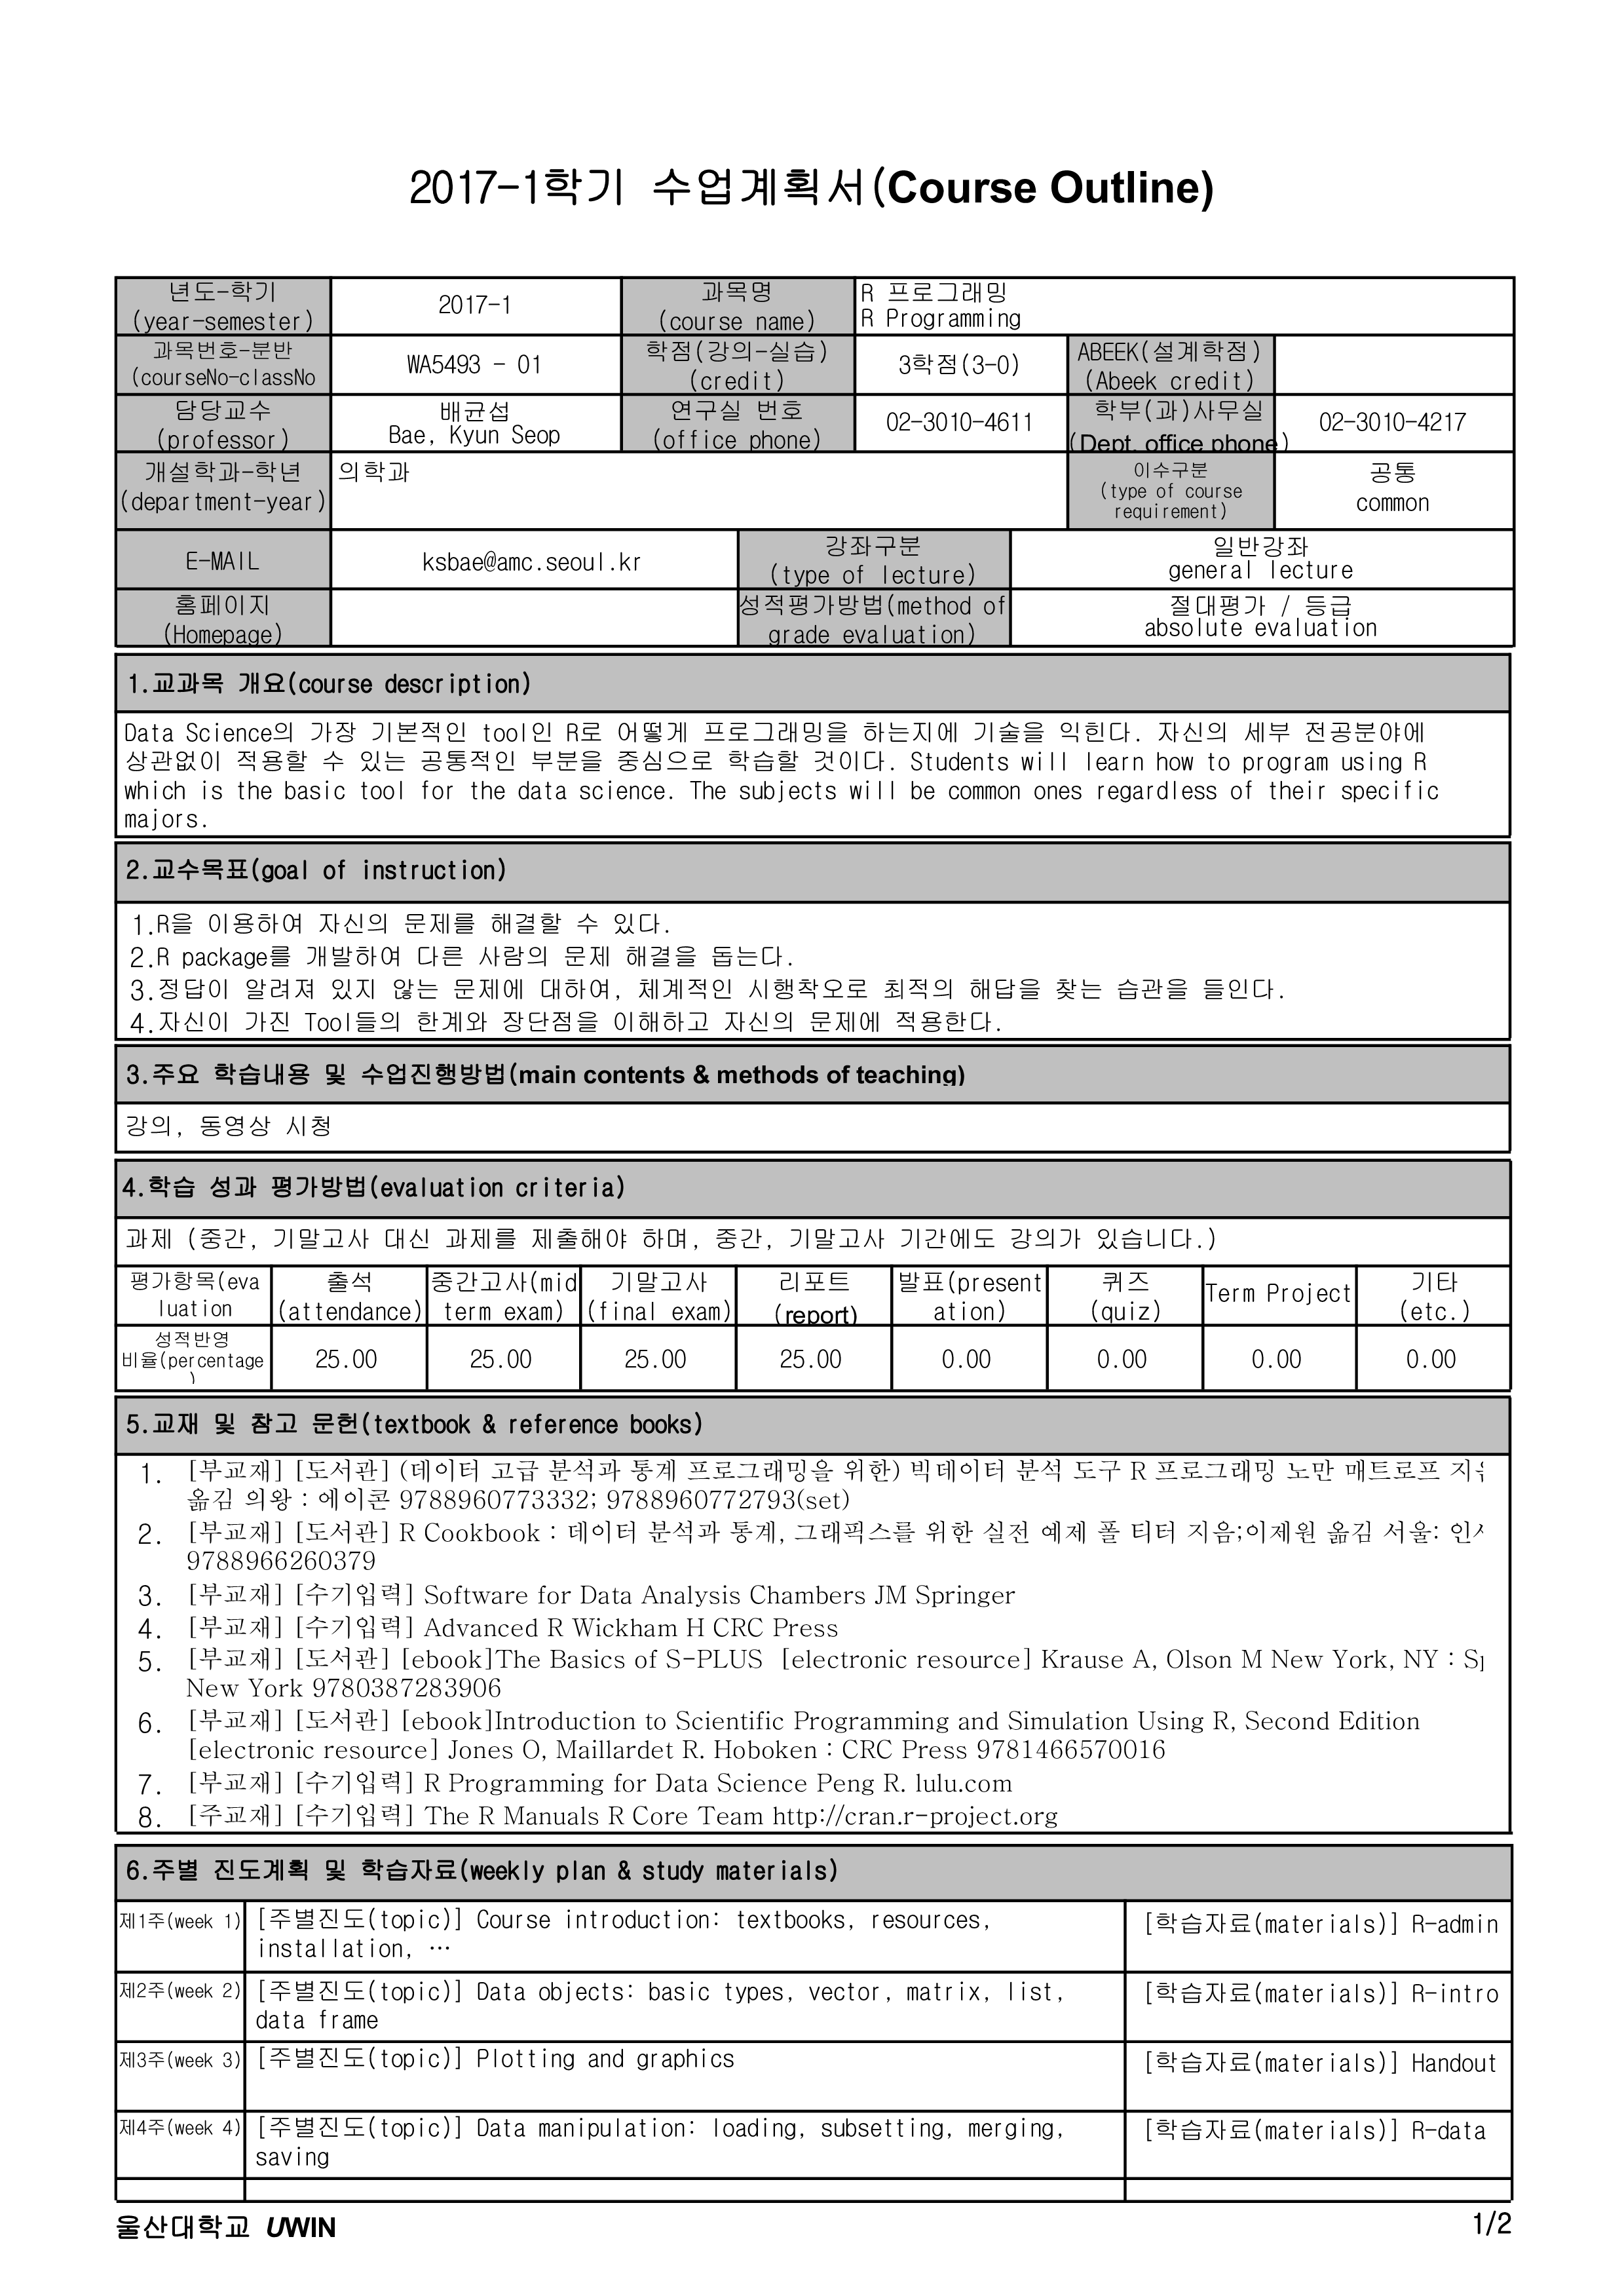
\includegraphics{inst/syllabus/syllabus_rev-0.png}
\caption{Syllabus page 1}
\end{figure}

\begin{figure}
\centering
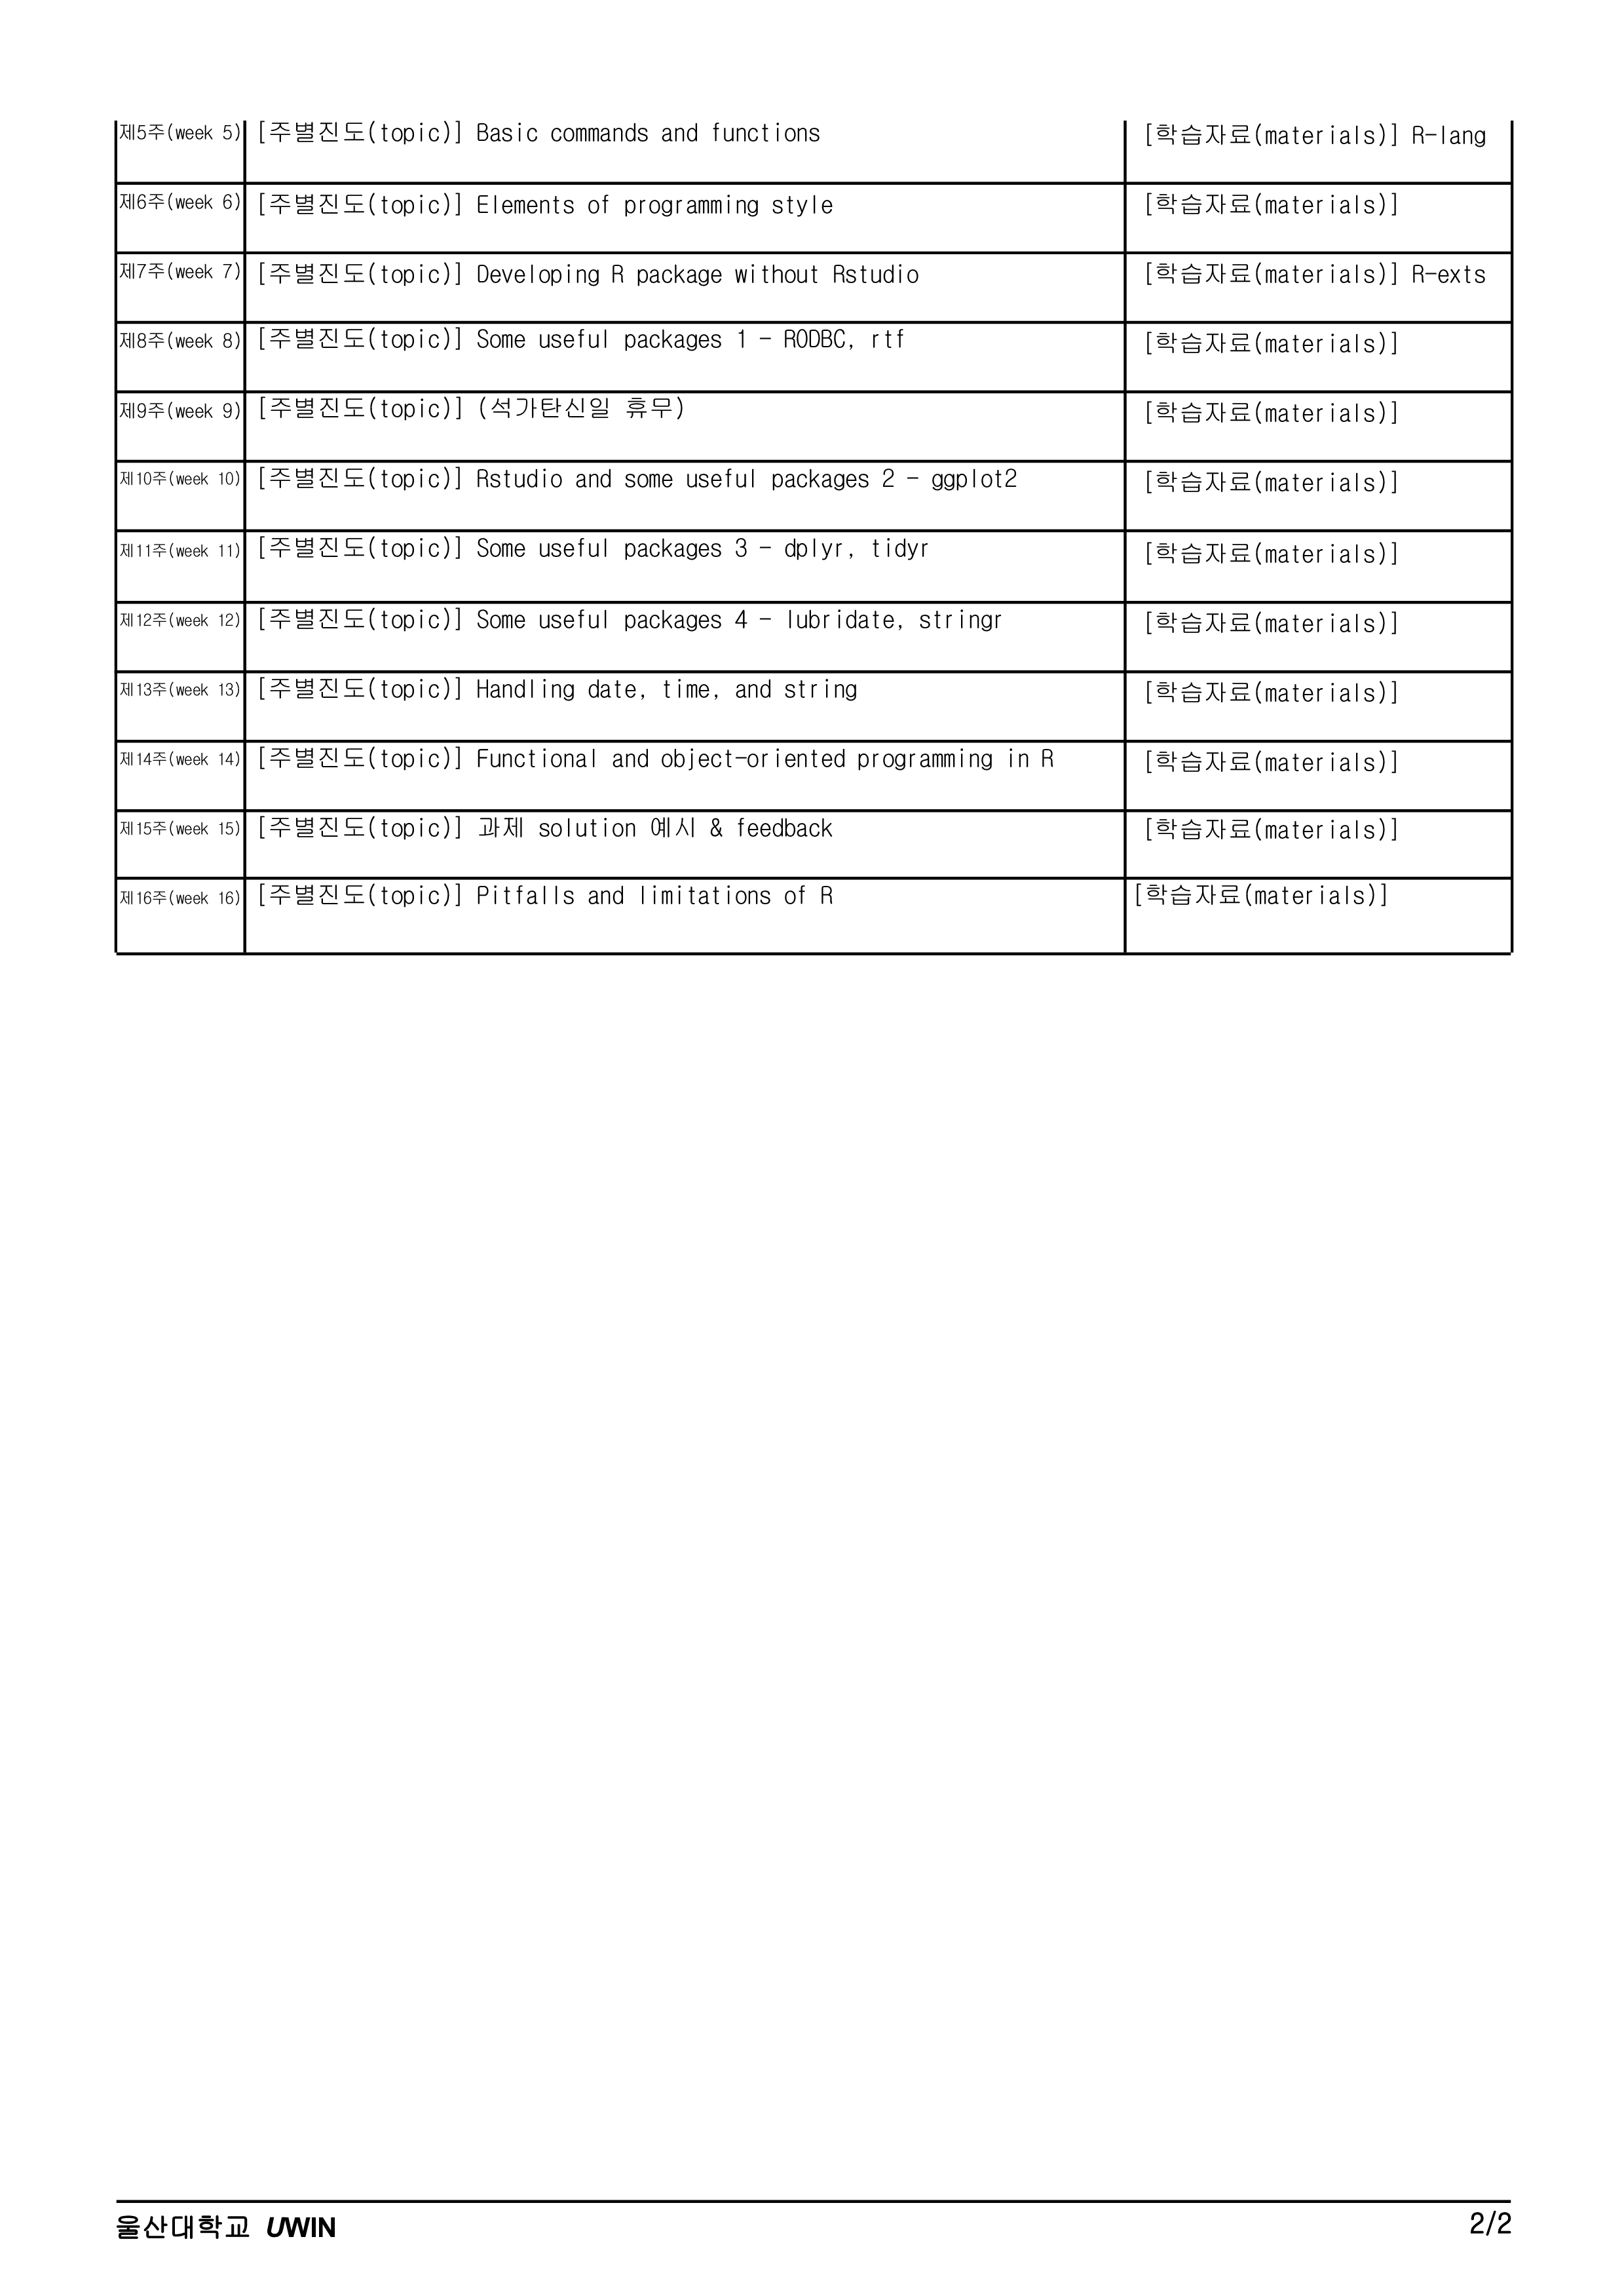
\includegraphics{inst/syllabus/syllabus_rev-1.png}
\caption{Syllabus page 1}
\end{figure}

\mainmatter

\chapter{R language}\label{r-language}

\begin{quote}
2017-03-15 배균섭 교수님 강의
\end{quote}

\href{https://cran.r-project.org/doc/manuals/r-release/R-lang.pdf}{R
Language Definition}의 초반 내용에 대해 설명하였습니다.

\chapter{Graphics}\label{graphics}

\begin{quote}
2017-03-22 임형석 교수님 강의
\end{quote}

R을 사용해 그림 그리는 방법에 대해 알아보겠습니다.

\section{Introduction}\label{introduction}

R에서 상위수준 그림 함수는 그림을 생성합니다. 반면 하위수준 그림 함수는
기존의 그림에 그림을 추가합니다.

\section{상위수준 그림 함수}\label{upper}

\subsection{상위수준 그림 함수의 주요 인자
(arguments)}\label{-----arguments}

\begin{itemize}
\tightlist
\item
  main : 제목
\item
  xlab/ylab : x축 및 y축 레이블
\item
  xlim/ylim : x축 및 y축 범위
\item
  col : 색깔
\item
  lty : 선 모양
\item
  pch : 점 모양
\item
  cex : 그림 성분의 크기
\item
  lwd : 선 굵기
\item
  type : 그림 타입
\end{itemize}

\begin{Shaded}
\begin{Highlighting}[]
\NormalTok{dta <-}\StringTok{ }\KeywordTok{read.csv}\NormalTok{(}\StringTok{"PK.csv"}\NormalTok{)}
\KeywordTok{head}\NormalTok{(dta)}
\end{Highlighting}
\end{Shaded}

\begin{verbatim}
##   ID TIME AMT    DV MDV
## 1  1 0.00   0  0.00   0
## 2  1 0.00   4  0.00   1
## 3  1 0.33   0  9.40   0
## 4  1 0.66   0 13.71   0
## 5  1 1.00   0 16.52   0
## 6  1 1.50   0 29.36   0
\end{verbatim}

\begin{Shaded}
\begin{Highlighting}[]
\KeywordTok{str}\NormalTok{(dta)}
\end{Highlighting}
\end{Shaded}

\begin{verbatim}
## 'data.frame':    456 obs. of  5 variables:
##  $ ID  : num  1 1 1 1 1 1 1 1 1 1 ...
##  $ TIME: num  0 0 0.33 0.66 1 1.5 2 3 4 6 ...
##  $ AMT : num  0 4 0 0 0 0 0 0 0 0 ...
##  $ DV  : num  0 0 9.4 13.7 16.5 ...
##  $ MDV : num  0 1 0 0 0 0 0 0 0 0 ...
\end{verbatim}

\subsection{scatter plot}\label{scatter-plot}

\begin{Shaded}
\begin{Highlighting}[]
\KeywordTok{plot}\NormalTok{(dta}\OperatorTok{$}\NormalTok{TIME[dta}\OperatorTok{$}\NormalTok{MDV}\OperatorTok{==}\DecValTok{0}\NormalTok{], dta}\OperatorTok{$}\NormalTok{DV[dta}\OperatorTok{$}\NormalTok{MDV}\OperatorTok{==}\DecValTok{0}\NormalTok{])}
\end{Highlighting}
\end{Shaded}

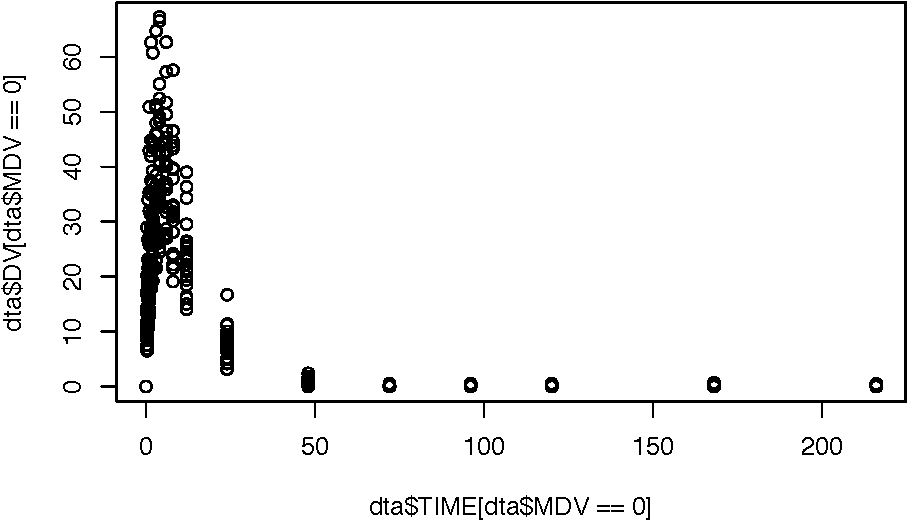
\includegraphics{Rprogramming_files/figure-latex/unnamed-chunk-3-1.pdf}

\begin{Shaded}
\begin{Highlighting}[]
\KeywordTok{plot}\NormalTok{(dta}\OperatorTok{$}\NormalTok{TIME[dta}\OperatorTok{$}\NormalTok{MDV}\OperatorTok{==}\DecValTok{0}\NormalTok{], dta}\OperatorTok{$}\NormalTok{DV[dta}\OperatorTok{$}\NormalTok{MDV}\OperatorTok{==}\DecValTok{0}\NormalTok{], }\DataTypeTok{log=}\StringTok{"y"}\NormalTok{)}
\end{Highlighting}
\end{Shaded}

\begin{verbatim}
## Warning in xy.coords(x, y, xlabel, ylabel, log): 86 y
## values <= 0 omitted from logarithmic plot
\end{verbatim}

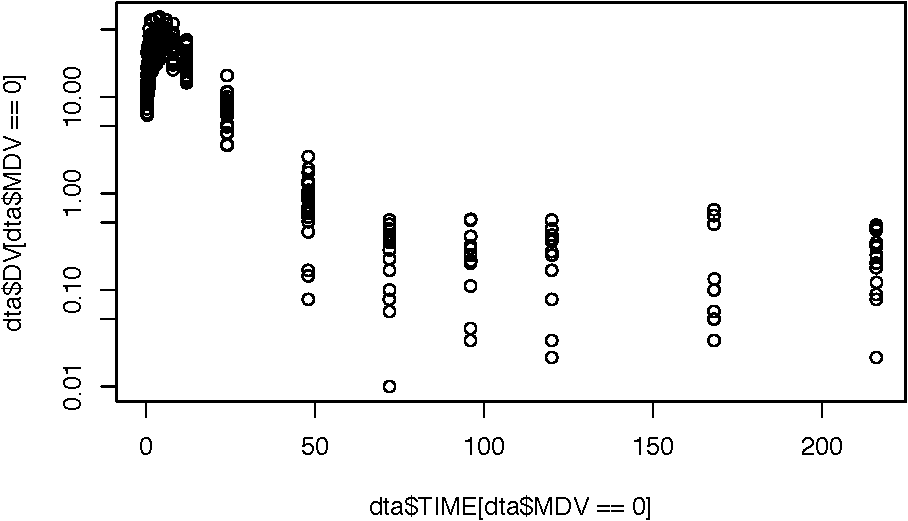
\includegraphics{Rprogramming_files/figure-latex/unnamed-chunk-3-2.pdf}

\begin{Shaded}
\begin{Highlighting}[]
\KeywordTok{plot}\NormalTok{(dta}\OperatorTok{$}\NormalTok{TIME[dta}\OperatorTok{$}\NormalTok{MDV}\OperatorTok{==}\DecValTok{0}\NormalTok{], }\KeywordTok{log}\NormalTok{(dta}\OperatorTok{$}\NormalTok{DV[dta}\OperatorTok{$}\NormalTok{MDV}\OperatorTok{==}\DecValTok{0}\NormalTok{]))}
\end{Highlighting}
\end{Shaded}

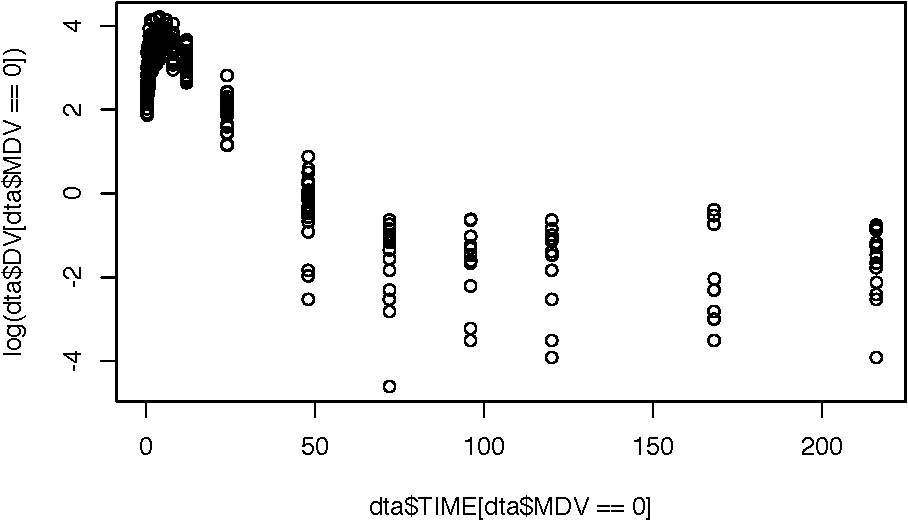
\includegraphics{Rprogramming_files/figure-latex/unnamed-chunk-3-3.pdf}

\begin{Shaded}
\begin{Highlighting}[]
\KeywordTok{plot}\NormalTok{(dta}\OperatorTok{$}\NormalTok{TIME[dta}\OperatorTok{$}\NormalTok{MDV}\OperatorTok{==}\DecValTok{0}\NormalTok{], dta}\OperatorTok{$}\NormalTok{DV[dta}\OperatorTok{$}\NormalTok{MDV}\OperatorTok{==}\DecValTok{0}\NormalTok{]}
\NormalTok{     , }\DataTypeTok{xlab=}\StringTok{"Time (hr)"}\NormalTok{, }\DataTypeTok{ylab=}\StringTok{"Concentration (ng/mL)"} 
\NormalTok{     , }\DataTypeTok{type=}\StringTok{"o"}\NormalTok{, }\DataTypeTok{pch=}\DecValTok{2}\NormalTok{, }\DataTypeTok{col=}\DecValTok{1}\NormalTok{, }\DataTypeTok{main=}\StringTok{"PK time-course of Drug X"}
\NormalTok{     , }\DataTypeTok{xlim =}\KeywordTok{c}\NormalTok{(}\OperatorTok{-}\DecValTok{2}\NormalTok{,}\DecValTok{218}\NormalTok{), }\DataTypeTok{ylim=}\KeywordTok{c}\NormalTok{(}\DecValTok{0}\NormalTok{,}\DecValTok{80}\NormalTok{))}
\end{Highlighting}
\end{Shaded}

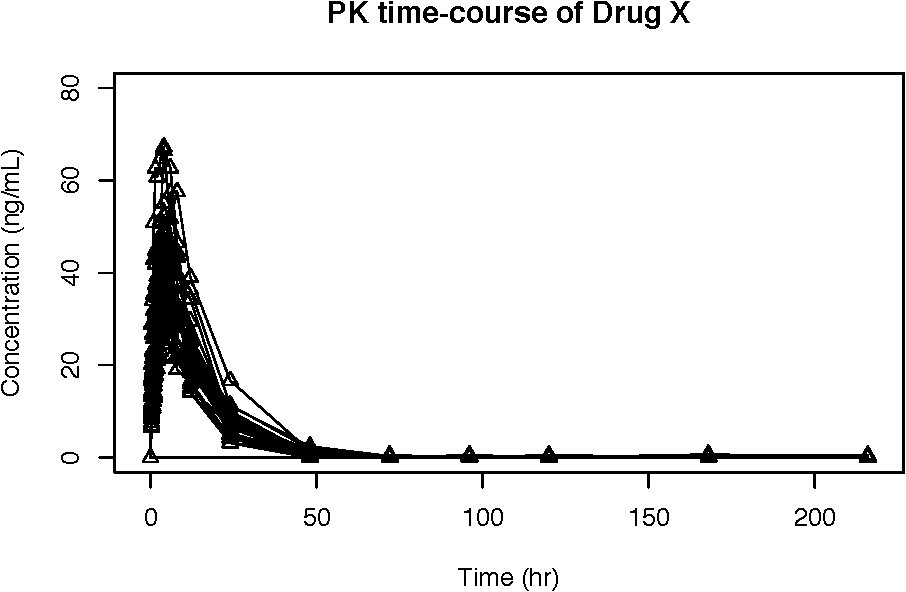
\includegraphics{Rprogramming_files/figure-latex/unnamed-chunk-3-4.pdf}

\begin{Shaded}
\begin{Highlighting}[]
\KeywordTok{plot}\NormalTok{(dta}\OperatorTok{$}\NormalTok{TIME[dta}\OperatorTok{$}\NormalTok{MDV}\OperatorTok{==}\DecValTok{0}\NormalTok{], dta}\OperatorTok{$}\NormalTok{DV[dta}\OperatorTok{$}\NormalTok{MDV}\OperatorTok{==}\DecValTok{0}\NormalTok{], }\DataTypeTok{axes=}\NormalTok{F,}
\NormalTok{     , }\DataTypeTok{xlab=}\StringTok{"Time (hr)"}\NormalTok{, }\DataTypeTok{ylab=}\StringTok{"Concentration (ng/mL)"} 
\NormalTok{     , }\DataTypeTok{type=}\StringTok{"o"}\NormalTok{, }\DataTypeTok{pch=}\DecValTok{2}\NormalTok{, }\DataTypeTok{col=}\DecValTok{1}\NormalTok{, }\DataTypeTok{main=}\StringTok{"PK time-course of Drug X"}
\NormalTok{     , }\DataTypeTok{xlim =}\KeywordTok{c}\NormalTok{(}\OperatorTok{-}\DecValTok{2}\NormalTok{,}\DecValTok{218}\NormalTok{), }\DataTypeTok{ylim=}\KeywordTok{c}\NormalTok{(}\DecValTok{0}\NormalTok{,}\DecValTok{80}\NormalTok{))}
\KeywordTok{axis}\NormalTok{(}\DecValTok{1}\NormalTok{, }\DataTypeTok{at=}\KeywordTok{seq}\NormalTok{(}\DecValTok{0}\NormalTok{, }\DecValTok{218}\NormalTok{, }\DecValTok{24}\NormalTok{))}
\KeywordTok{axis}\NormalTok{(}\DecValTok{2}\NormalTok{)}
\KeywordTok{box}\NormalTok{()}
\end{Highlighting}
\end{Shaded}

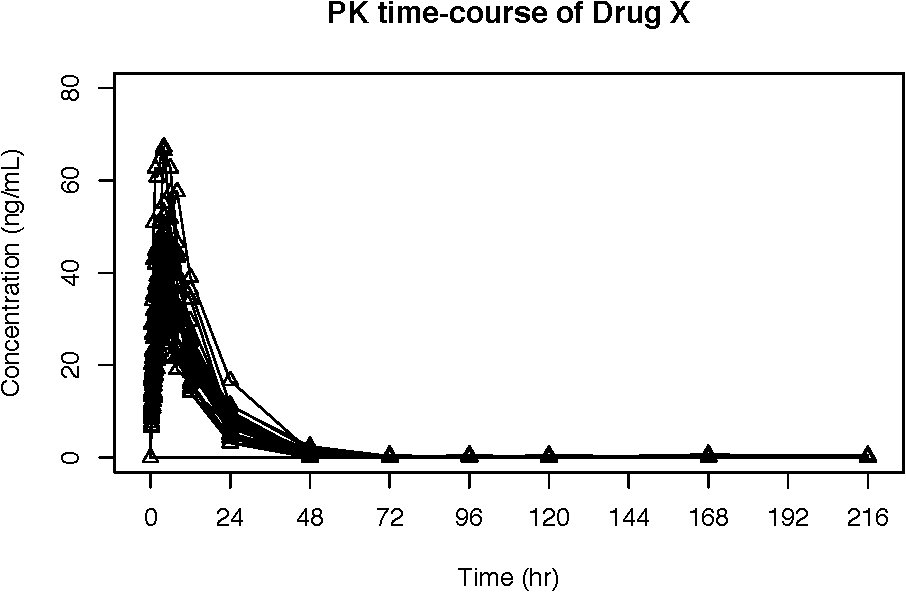
\includegraphics{Rprogramming_files/figure-latex/unnamed-chunk-3-5.pdf}

\subsection{Histogram}\label{histogram}

\begin{Shaded}
\begin{Highlighting}[]
\NormalTok{d.demog <-}\StringTok{ }\KeywordTok{read.csv}\NormalTok{(}\StringTok{"DEMOG.csv"}\NormalTok{)}

\KeywordTok{hist}\NormalTok{(d.demog}\OperatorTok{$}\NormalTok{HT)}
\end{Highlighting}
\end{Shaded}

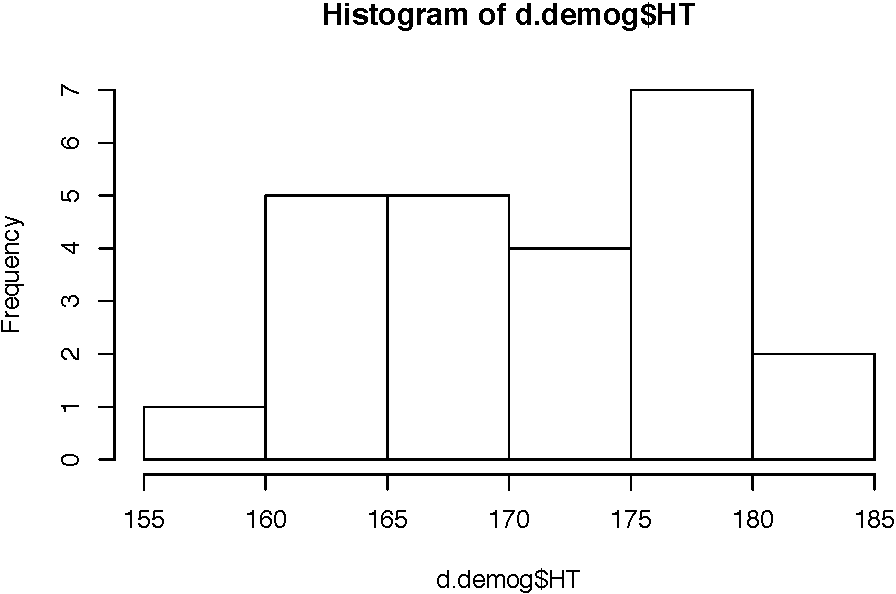
\includegraphics{Rprogramming_files/figure-latex/unnamed-chunk-4-1.pdf}

\begin{Shaded}
\begin{Highlighting}[]
\KeywordTok{hist}\NormalTok{(d.demog}\OperatorTok{$}\NormalTok{HT, }\DataTypeTok{breaks=}\DecValTok{10}\NormalTok{)}
\KeywordTok{hist}\NormalTok{(d.demog}\OperatorTok{$}\NormalTok{HT, }\DataTypeTok{nclass=}\DecValTok{10}\NormalTok{)}
\end{Highlighting}
\end{Shaded}

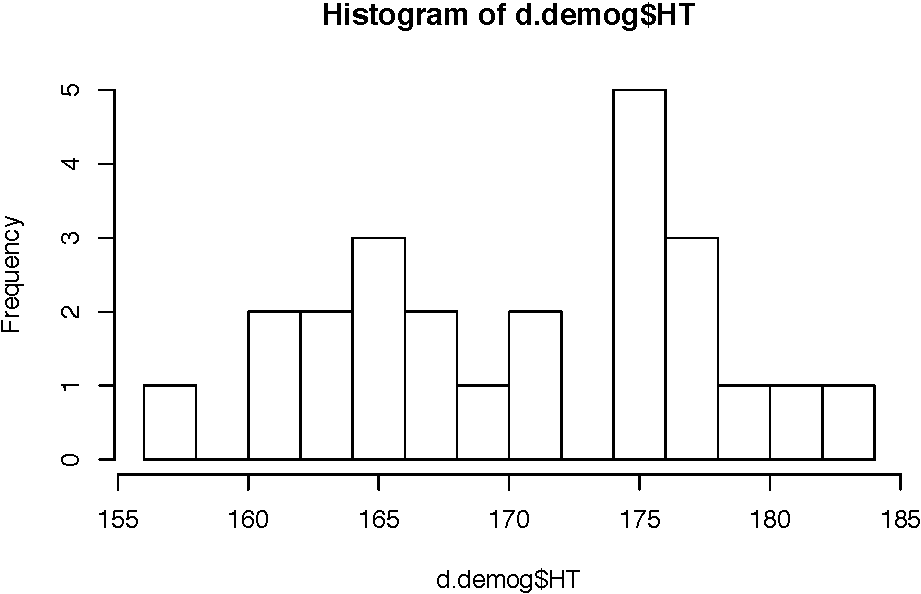
\includegraphics{Rprogramming_files/figure-latex/unnamed-chunk-4-2.pdf}

\subsubsection{with density line}\label{with-density-line}

\begin{Shaded}
\begin{Highlighting}[]
\KeywordTok{hist}\NormalTok{ (d.demog}\OperatorTok{$}\NormalTok{HT, }\DataTypeTok{probability=}\OtherTok{TRUE}\NormalTok{, }\DataTypeTok{breaks=}\DecValTok{10}\NormalTok{)}
\KeywordTok{lines}\NormalTok{(}\KeywordTok{density}\NormalTok{(d.demog}\OperatorTok{$}\NormalTok{HT))}
\end{Highlighting}
\end{Shaded}

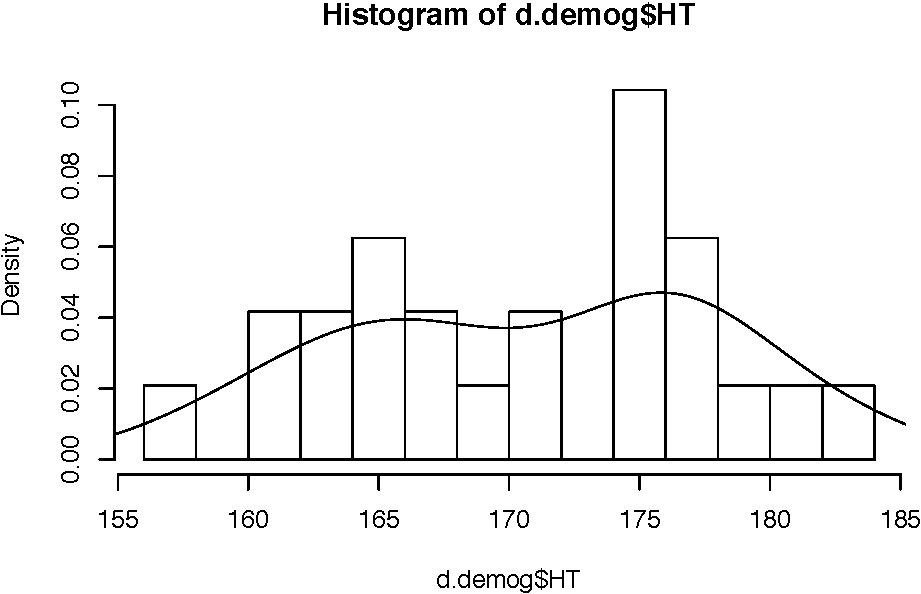
\includegraphics{Rprogramming_files/figure-latex/unnamed-chunk-5-1.pdf}

\begin{Shaded}
\begin{Highlighting}[]
\KeywordTok{hist}\NormalTok{ (d.demog}\OperatorTok{$}\NormalTok{HT, }\DataTypeTok{probability=}\OtherTok{TRUE}\NormalTok{, }\DataTypeTok{breaks=}\DecValTok{9}\NormalTok{, }\DataTypeTok{xaxt=}\StringTok{"n"}
\NormalTok{      , }\DataTypeTok{main=}\StringTok{"Histogram for Height"}\NormalTok{, }\DataTypeTok{xlab=}\StringTok{"Height (cm)"}\NormalTok{, }\DataTypeTok{ylab=}\StringTok{"Probability (%)"}\NormalTok{)}
\KeywordTok{axis}\NormalTok{(}\DecValTok{1}\NormalTok{, }\DataTypeTok{at=}\KeywordTok{seq}\NormalTok{(}\KeywordTok{min}\NormalTok{(d.demog}\OperatorTok{$}\NormalTok{HT), }\KeywordTok{max}\NormalTok{(d.demog}\OperatorTok{$}\NormalTok{HT), }\DecValTok{3}\NormalTok{))}
\KeywordTok{lines}\NormalTok{(}\KeywordTok{density}\NormalTok{(d.demog}\OperatorTok{$}\NormalTok{HT))}
\end{Highlighting}
\end{Shaded}

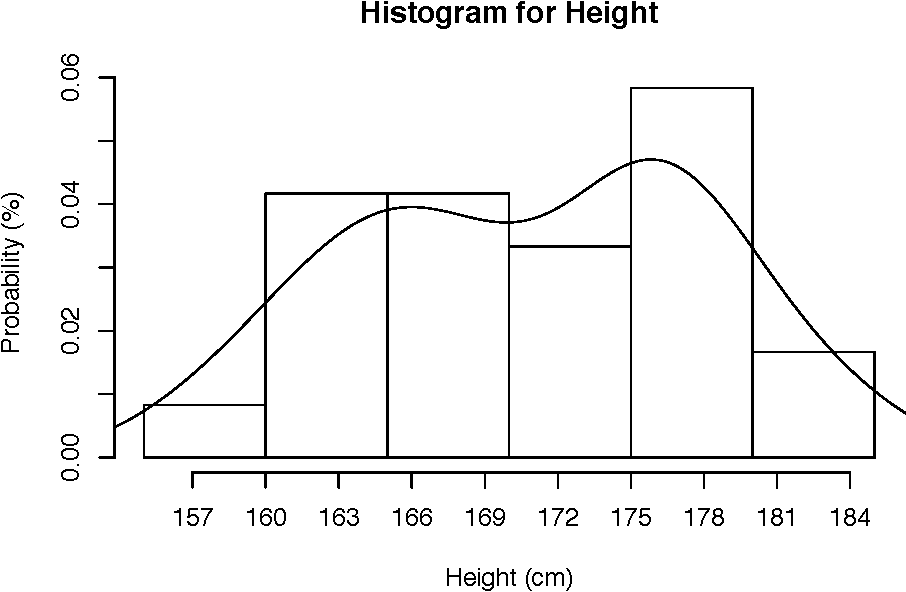
\includegraphics{Rprogramming_files/figure-latex/unnamed-chunk-5-2.pdf}

\begin{Shaded}
\begin{Highlighting}[]
\KeywordTok{hist}\NormalTok{ (d.demog}\OperatorTok{$}\NormalTok{HT, }\DataTypeTok{probability=}\OtherTok{TRUE}\NormalTok{, }\DataTypeTok{breaks=}\DecValTok{9}\NormalTok{, }\DataTypeTok{xaxt=}\StringTok{"n"}
\NormalTok{      , }\DataTypeTok{main=}\StringTok{"Histogram for Height"}\NormalTok{, }\DataTypeTok{xlab=}\StringTok{"Height (cm)"}\NormalTok{, }\DataTypeTok{ylab=}\StringTok{"Probability (%)"}
\NormalTok{      , }\DataTypeTok{col =} \StringTok{"lightblue"}\NormalTok{, }\DataTypeTok{border =} \StringTok{"pink"}\NormalTok{)}
\KeywordTok{axis}\NormalTok{(}\DecValTok{1}\NormalTok{, }\DataTypeTok{at=}\KeywordTok{seq}\NormalTok{(}\KeywordTok{min}\NormalTok{(d.demog}\OperatorTok{$}\NormalTok{HT), }\KeywordTok{max}\NormalTok{(d.demog}\OperatorTok{$}\NormalTok{HT), }\DecValTok{3}\NormalTok{))}
\KeywordTok{lines}\NormalTok{(}\KeywordTok{density}\NormalTok{(d.demog}\OperatorTok{$}\NormalTok{HT))}
\end{Highlighting}
\end{Shaded}

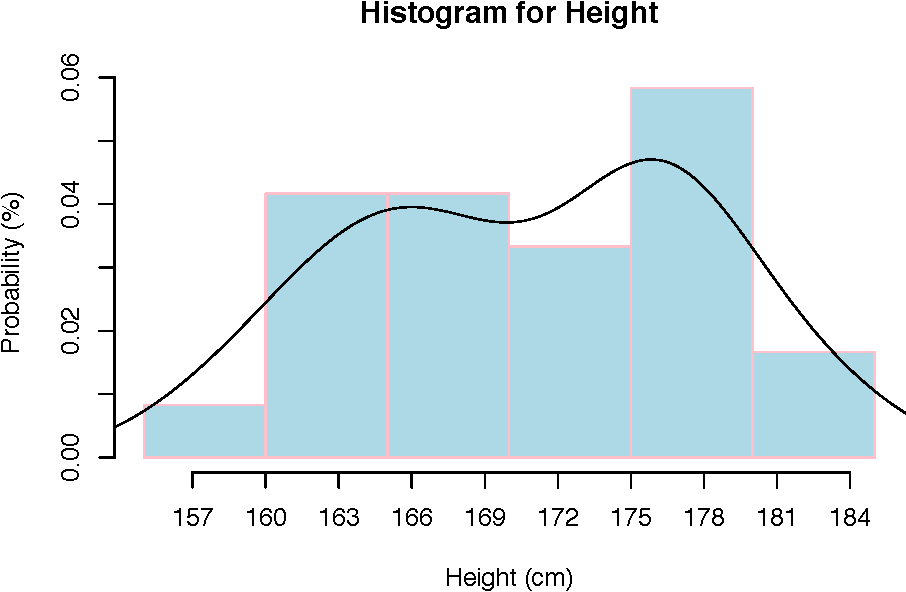
\includegraphics{Rprogramming_files/figure-latex/unnamed-chunk-5-3.pdf}

\subsection{Box-Whisker Plot}\label{box-whisker-plot}

\begin{Shaded}
\begin{Highlighting}[]
\KeywordTok{boxplot}\NormalTok{(d.demog}\OperatorTok{$}\NormalTok{WT)}
\end{Highlighting}
\end{Shaded}

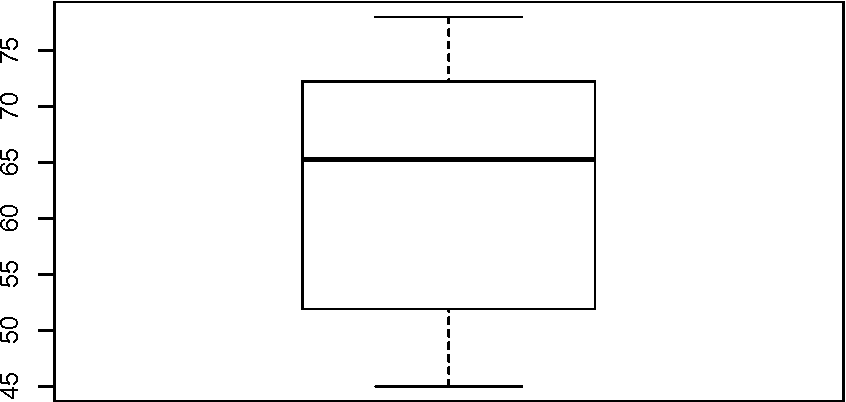
\includegraphics{Rprogramming_files/figure-latex/unnamed-chunk-6-1.pdf}

\begin{Shaded}
\begin{Highlighting}[]
\KeywordTok{boxplot}\NormalTok{(d.demog}\OperatorTok{$}\NormalTok{WT }\OperatorTok{~}\StringTok{ }\NormalTok{d.demog}\OperatorTok{$}\NormalTok{SEX)}

\KeywordTok{boxplot}\NormalTok{(}\KeywordTok{split}\NormalTok{(d.demog}\OperatorTok{$}\NormalTok{WT, d.demog}\OperatorTok{$}\NormalTok{SEX))}
\end{Highlighting}
\end{Shaded}

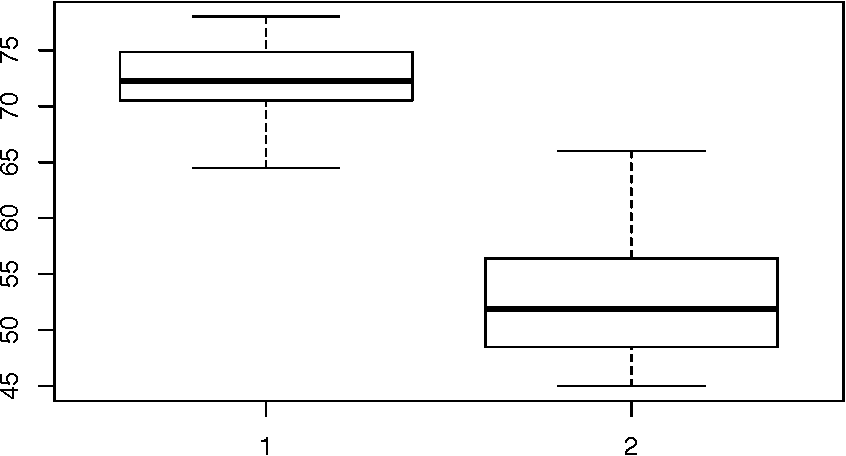
\includegraphics{Rprogramming_files/figure-latex/unnamed-chunk-6-2.pdf}

\begin{Shaded}
\begin{Highlighting}[]
\KeywordTok{boxplot}\NormalTok{(WT }\OperatorTok{~}\StringTok{ }\NormalTok{SEX, }\DataTypeTok{data=}\NormalTok{d.demog)}

\KeywordTok{boxplot}\NormalTok{(d.demog}\OperatorTok{$}\NormalTok{WT }\OperatorTok{~}\StringTok{ }\NormalTok{d.demog}\OperatorTok{$}\NormalTok{SEX}
\NormalTok{        , }\DataTypeTok{names=}\KeywordTok{c}\NormalTok{(}\StringTok{"Male"}\NormalTok{,}\StringTok{"Female"}\NormalTok{), }\DataTypeTok{ylab=}\StringTok{"AGE, year"}\NormalTok{, }\DataTypeTok{ylim=}\KeywordTok{c}\NormalTok{(}\KeywordTok{min}\NormalTok{(d.demog}\OperatorTok{$}\NormalTok{WT)}\OperatorTok{-}\DecValTok{2}\NormalTok{, }\KeywordTok{max}\NormalTok{(d.demog}\OperatorTok{$}\NormalTok{WT)}\OperatorTok{+}\DecValTok{2}\NormalTok{)}
\NormalTok{        , }\DataTypeTok{col=}\StringTok{"pink"}\NormalTok{)}
\end{Highlighting}
\end{Shaded}

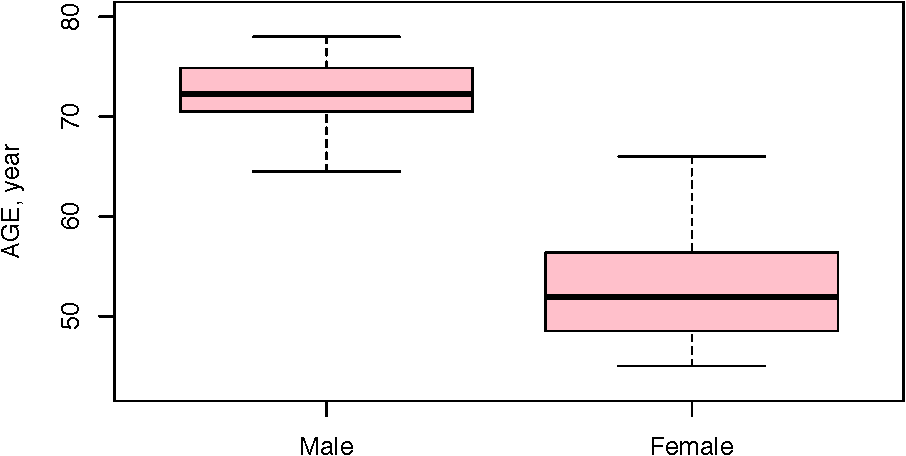
\includegraphics{Rprogramming_files/figure-latex/unnamed-chunk-6-3.pdf}

\begin{Shaded}
\begin{Highlighting}[]
\KeywordTok{boxplot}\NormalTok{(d.demog}\OperatorTok{$}\NormalTok{WT }\OperatorTok{~}\StringTok{ }\NormalTok{d.demog}\OperatorTok{$}\NormalTok{SEX}
\NormalTok{        , }\DataTypeTok{names=}\KeywordTok{c}\NormalTok{(}\StringTok{"Male"}\NormalTok{,}\StringTok{"Female"}\NormalTok{), }\DataTypeTok{ylab=}\StringTok{"AGE, year"}\NormalTok{, }\DataTypeTok{ylim=}\KeywordTok{c}\NormalTok{(}\KeywordTok{min}\NormalTok{(d.demog}\OperatorTok{$}\NormalTok{WT)}\OperatorTok{-}\DecValTok{2}\NormalTok{, }\KeywordTok{max}\NormalTok{(d.demog}\OperatorTok{$}\NormalTok{WT)}\OperatorTok{+}\DecValTok{2}\NormalTok{)}
\NormalTok{        , }\DataTypeTok{col=}\KeywordTok{c}\NormalTok{(}\StringTok{"lightblue"}\NormalTok{, }\StringTok{"salmon"}\NormalTok{), }\DataTypeTok{width=}\KeywordTok{c}\NormalTok{(}\FloatTok{0.6}\NormalTok{, }\DecValTok{1}\NormalTok{))}
\end{Highlighting}
\end{Shaded}

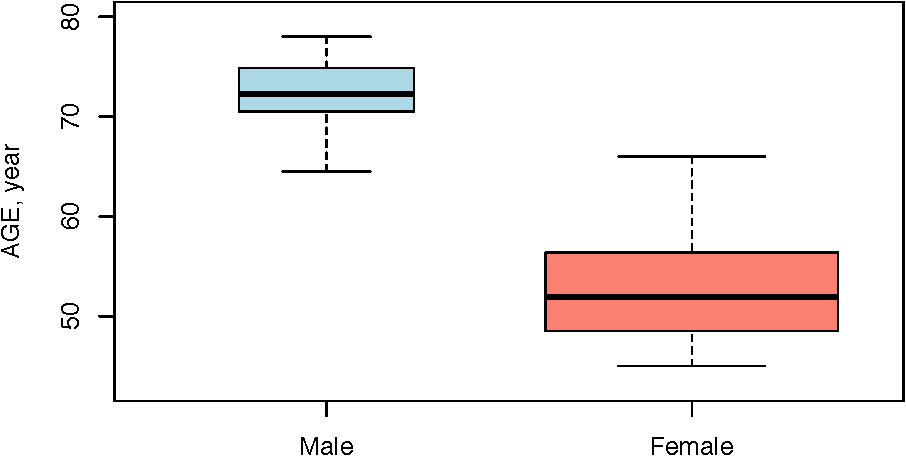
\includegraphics{Rprogramming_files/figure-latex/unnamed-chunk-6-4.pdf}

-varwidth: if varwidth is TRUE, the boxes are drawn with widths
proportional to the square-roots of the number of observations in the
groups.

\begin{Shaded}
\begin{Highlighting}[]
\KeywordTok{boxplot}\NormalTok{(d.demog}\OperatorTok{$}\NormalTok{WT }\OperatorTok{~}\StringTok{ }\NormalTok{d.demog}\OperatorTok{$}\NormalTok{SEX}
\NormalTok{        , }\DataTypeTok{names=}\KeywordTok{c}\NormalTok{(}\StringTok{"Male"}\NormalTok{,}\StringTok{"Female"}\NormalTok{), }\DataTypeTok{ylab=}\StringTok{"AGE, year"}\NormalTok{, }\DataTypeTok{ylim=}\KeywordTok{c}\NormalTok{(}\KeywordTok{min}\NormalTok{(d.demog}\OperatorTok{$}\NormalTok{WT)}\OperatorTok{-}\DecValTok{2}\NormalTok{, }\KeywordTok{max}\NormalTok{(d.demog}\OperatorTok{$}\NormalTok{WT)}\OperatorTok{+}\DecValTok{2}\NormalTok{)}
\NormalTok{        , }\DataTypeTok{col=}\KeywordTok{c}\NormalTok{(}\StringTok{"lightblue"}\NormalTok{, }\StringTok{"salmon"}\NormalTok{)}
\NormalTok{        , }\DataTypeTok{varwidth=}\OtherTok{TRUE}\NormalTok{)}
\end{Highlighting}
\end{Shaded}

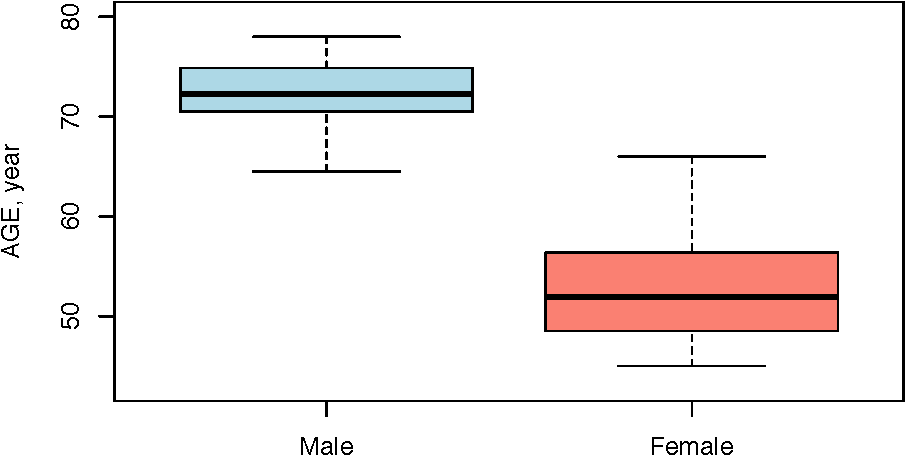
\includegraphics{Rprogramming_files/figure-latex/unnamed-chunk-7-1.pdf}

\subsection{Bar Plot}\label{bar-plot}

\begin{Shaded}
\begin{Highlighting}[]
\KeywordTok{barplot}\NormalTok{(d.demog}\OperatorTok{$}\NormalTok{HT)}
\end{Highlighting}
\end{Shaded}

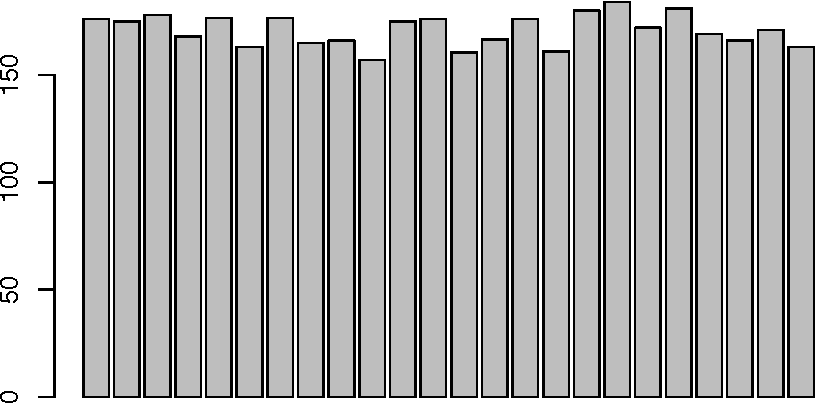
\includegraphics{Rprogramming_files/figure-latex/unnamed-chunk-8-1.pdf}

\begin{Shaded}
\begin{Highlighting}[]
\NormalTok{VADeaths}
\end{Highlighting}
\end{Shaded}

\begin{verbatim}
##       Rural Male Rural Female Urban Male Urban Female
## 50-54       11.7          8.7       15.4          8.4
## 55-59       18.1         11.7       24.3         13.6
## 60-64       26.9         20.3       37.0         19.3
## 65-69       41.0         30.9       54.6         35.1
## 70-74       66.0         54.3       71.1         50.0
\end{verbatim}

\begin{Shaded}
\begin{Highlighting}[]
\KeywordTok{barplot}\NormalTok{(VADeaths, }\DataTypeTok{border =} \StringTok{"dark blue"}\NormalTok{)}
\end{Highlighting}
\end{Shaded}

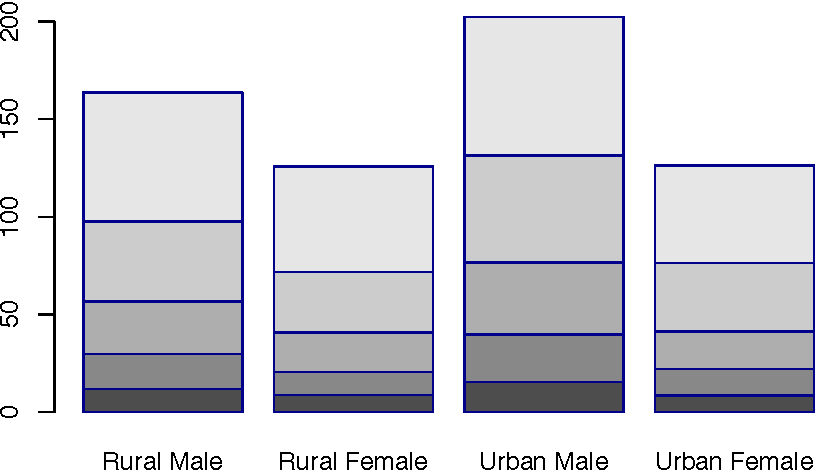
\includegraphics{Rprogramming_files/figure-latex/unnamed-chunk-8-2.pdf}

\begin{Shaded}
\begin{Highlighting}[]
\KeywordTok{barplot}\NormalTok{(VADeaths, }\DataTypeTok{col =} \KeywordTok{rainbow}\NormalTok{(}\DecValTok{20}\NormalTok{))}
\end{Highlighting}
\end{Shaded}

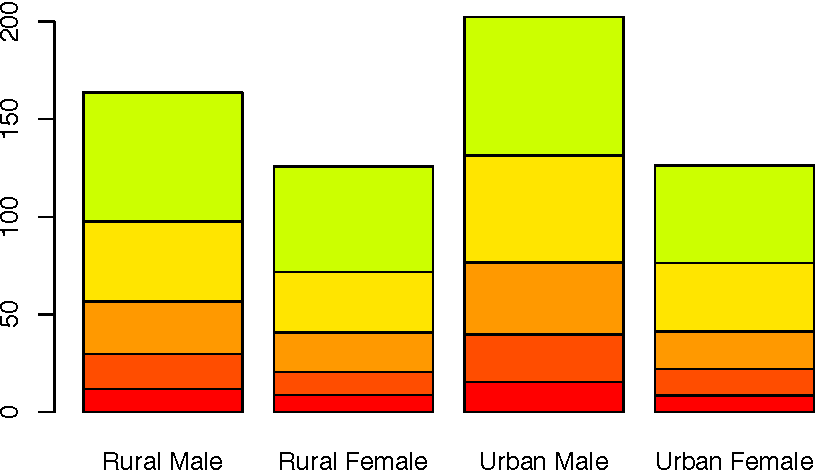
\includegraphics{Rprogramming_files/figure-latex/unnamed-chunk-8-3.pdf}

\begin{Shaded}
\begin{Highlighting}[]
\KeywordTok{barplot}\NormalTok{(VADeaths, }\DataTypeTok{col =} \KeywordTok{heat.colors}\NormalTok{(}\DecValTok{8}\NormalTok{))}
\end{Highlighting}
\end{Shaded}

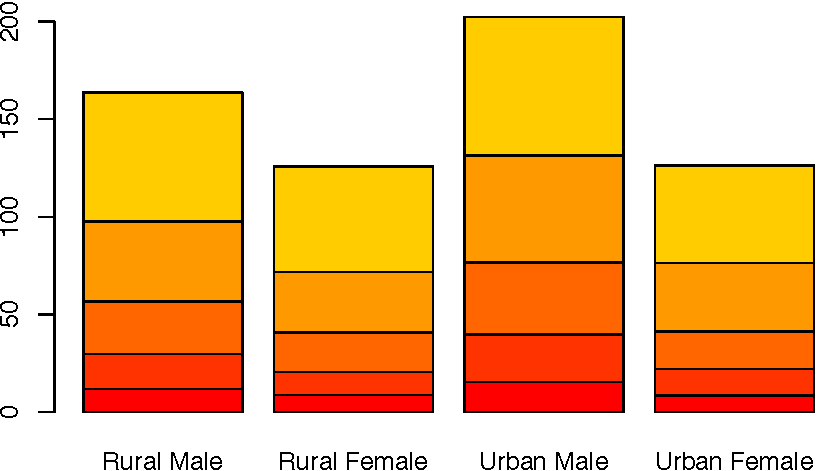
\includegraphics{Rprogramming_files/figure-latex/unnamed-chunk-8-4.pdf}

\begin{Shaded}
\begin{Highlighting}[]
\KeywordTok{barplot}\NormalTok{(VADeaths, }\DataTypeTok{col =} \KeywordTok{gray.colors}\NormalTok{(}\DecValTok{4}\NormalTok{))}
\end{Highlighting}
\end{Shaded}

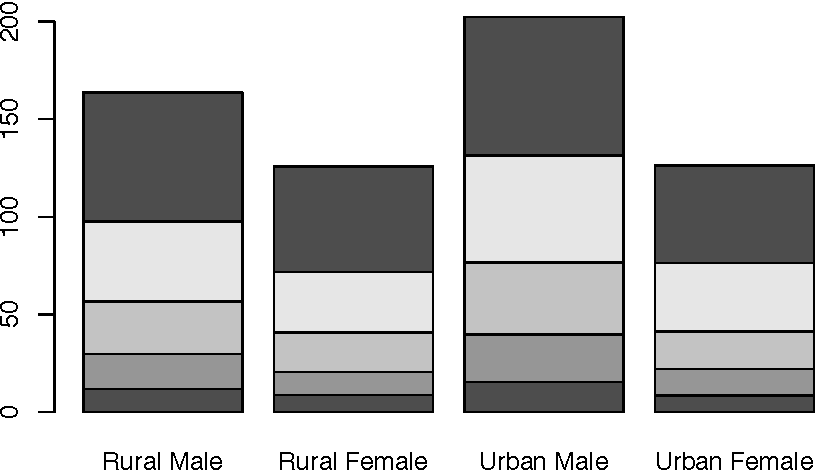
\includegraphics{Rprogramming_files/figure-latex/unnamed-chunk-8-5.pdf}

\begin{Shaded}
\begin{Highlighting}[]
\KeywordTok{barplot}\NormalTok{(VADeaths, }\DataTypeTok{col =} \KeywordTok{gray.colors}\NormalTok{(}\DecValTok{4}\NormalTok{), }\DataTypeTok{log=}\StringTok{"x"}\NormalTok{)}
\end{Highlighting}
\end{Shaded}

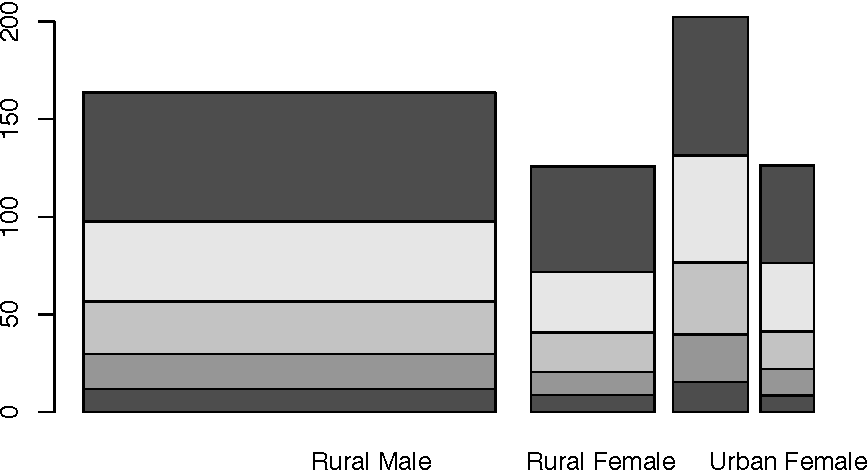
\includegraphics{Rprogramming_files/figure-latex/unnamed-chunk-8-6.pdf}

\begin{Shaded}
\begin{Highlighting}[]
\KeywordTok{barplot}\NormalTok{(VADeaths, }\DataTypeTok{col =} \KeywordTok{gray.colors}\NormalTok{(}\DecValTok{4}\NormalTok{), }\DataTypeTok{log=}\StringTok{"y"}\NormalTok{)}
\end{Highlighting}
\end{Shaded}

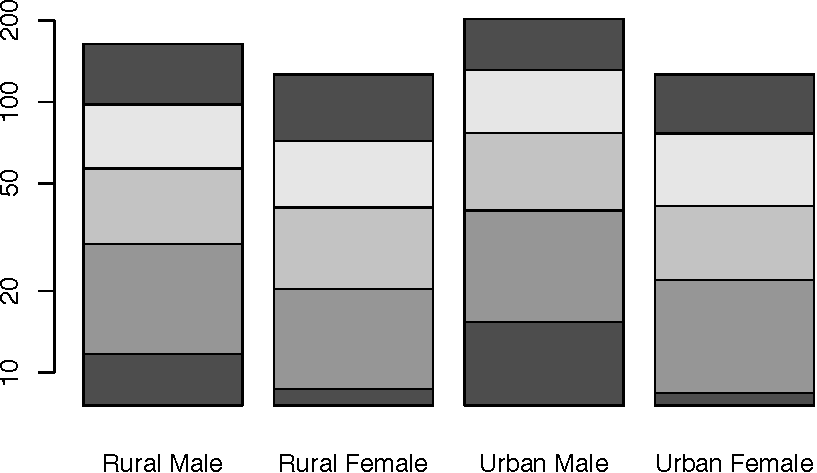
\includegraphics{Rprogramming_files/figure-latex/unnamed-chunk-8-7.pdf}

\begin{Shaded}
\begin{Highlighting}[]
\KeywordTok{barplot}\NormalTok{(VADeaths, }\DataTypeTok{col =} \KeywordTok{gray.colors}\NormalTok{(}\DecValTok{4}\NormalTok{), }\DataTypeTok{log=}\StringTok{"xy"}\NormalTok{)}
\end{Highlighting}
\end{Shaded}

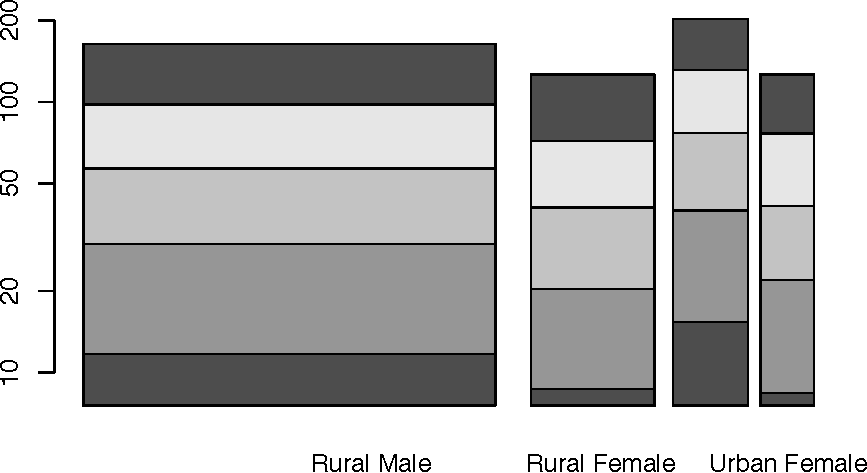
\includegraphics{Rprogramming_files/figure-latex/unnamed-chunk-8-8.pdf}

\subsection{pie chart}\label{pie-chart}

\begin{Shaded}
\begin{Highlighting}[]
\NormalTok{drug.X.market <-}\StringTok{ }\KeywordTok{c}\NormalTok{(}\FloatTok{0.12}\NormalTok{, }\FloatTok{0.29}\NormalTok{, }\FloatTok{0.32}\NormalTok{, }\FloatTok{0.22}\NormalTok{, }\FloatTok{0.11}\NormalTok{, }\FloatTok{0.28}\NormalTok{)}
\KeywordTok{names}\NormalTok{(drug.X.market) <-}\StringTok{ }\KeywordTok{c}\NormalTok{(}\StringTok{"South Korea"}\NormalTok{,}\StringTok{"China"}\NormalTok{,}\StringTok{"USA"}\NormalTok{,}\StringTok{"Japan"}\NormalTok{,}\StringTok{"Austria"}\NormalTok{,}\StringTok{"EU"}\NormalTok{)}
\KeywordTok{pie}\NormalTok{(drug.X.market)}
\end{Highlighting}
\end{Shaded}

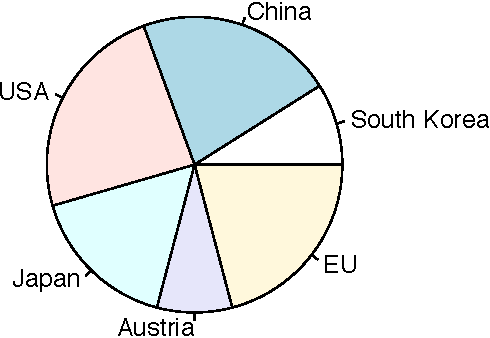
\includegraphics{Rprogramming_files/figure-latex/unnamed-chunk-9-1.pdf}

\subsection{matplot 함수}\label{matplot-}

\subsubsection{matrix와 column 사이의 그림}\label{matrix-column--}

\begin{Shaded}
\begin{Highlighting}[]
\NormalTok{pct.}\DecValTok{95}\NormalTok{ <-}\StringTok{ }\KeywordTok{read.csv}\NormalTok{(}\StringTok{"pct95.csv"}\NormalTok{)}
\KeywordTok{matplot}\NormalTok{(pct.}\DecValTok{95}\NormalTok{[,}\DecValTok{1}\NormalTok{], pct.}\DecValTok{95}\NormalTok{[,}\DecValTok{2}\OperatorTok{:}\KeywordTok{ncol}\NormalTok{(pct.}\DecValTok{95}\NormalTok{)], }\DataTypeTok{pch=}\DecValTok{1}\NormalTok{)}
\end{Highlighting}
\end{Shaded}

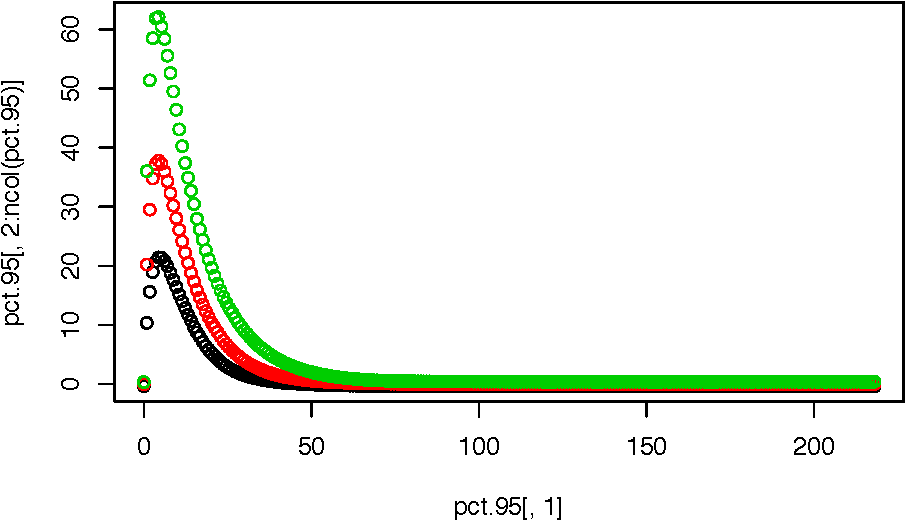
\includegraphics{Rprogramming_files/figure-latex/unnamed-chunk-10-1.pdf}

\begin{Shaded}
\begin{Highlighting}[]
\KeywordTok{matplot}\NormalTok{(pct.}\DecValTok{95}\NormalTok{[,}\DecValTok{1}\NormalTok{], pct.}\DecValTok{95}\NormalTok{[,}\DecValTok{2}\OperatorTok{:}\KeywordTok{ncol}\NormalTok{(pct.}\DecValTok{95}\NormalTok{)], }\DataTypeTok{pch=}\DecValTok{1}\NormalTok{, }\DataTypeTok{col=}\KeywordTok{c}\NormalTok{(}\DecValTok{1}\NormalTok{,}\DecValTok{2}\NormalTok{,}\DecValTok{1}\NormalTok{), }\DataTypeTok{type=}\StringTok{"l"}\NormalTok{, }\DataTypeTok{lty=}\DecValTok{1}\NormalTok{, }\DataTypeTok{lwd=}\KeywordTok{c}\NormalTok{(}\DecValTok{1}\NormalTok{,}\DecValTok{2}\NormalTok{,}\DecValTok{1}\NormalTok{))}
\end{Highlighting}
\end{Shaded}

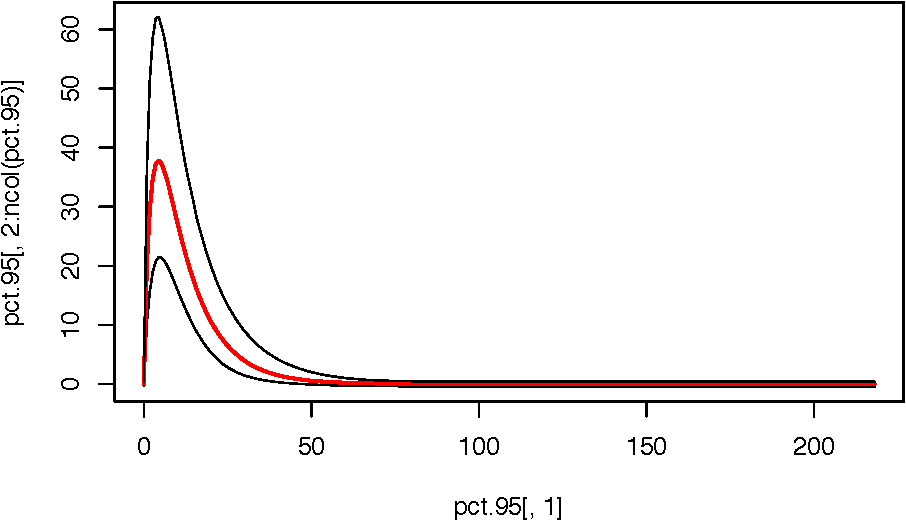
\includegraphics{Rprogramming_files/figure-latex/unnamed-chunk-10-2.pdf}

\subsection{Scatter plot matrices (pairs
plots)}\label{scatter-plot-matrices-pairs-plots}

\begin{Shaded}
\begin{Highlighting}[]
\KeywordTok{pairs}\NormalTok{(d.demog)}
\end{Highlighting}
\end{Shaded}

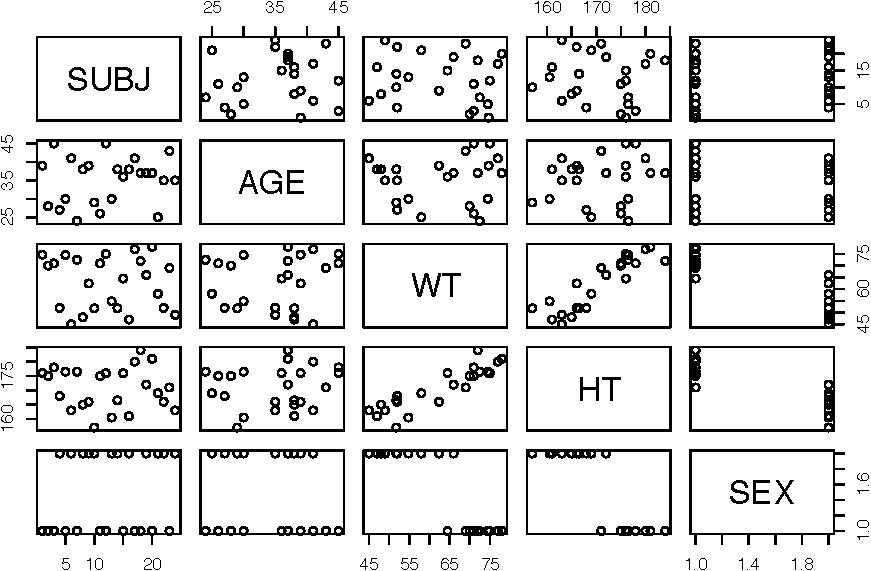
\includegraphics{Rprogramming_files/figure-latex/unnamed-chunk-11-1.pdf}

\subsubsection{add a loess smoother,
type}\label{add-a-loess-smoother-type}

\begin{Shaded}
\begin{Highlighting}[]
\KeywordTok{pairs}\NormalTok{(d.demog, }\DataTypeTok{panel =}\NormalTok{ panel.smooth)}
\end{Highlighting}
\end{Shaded}

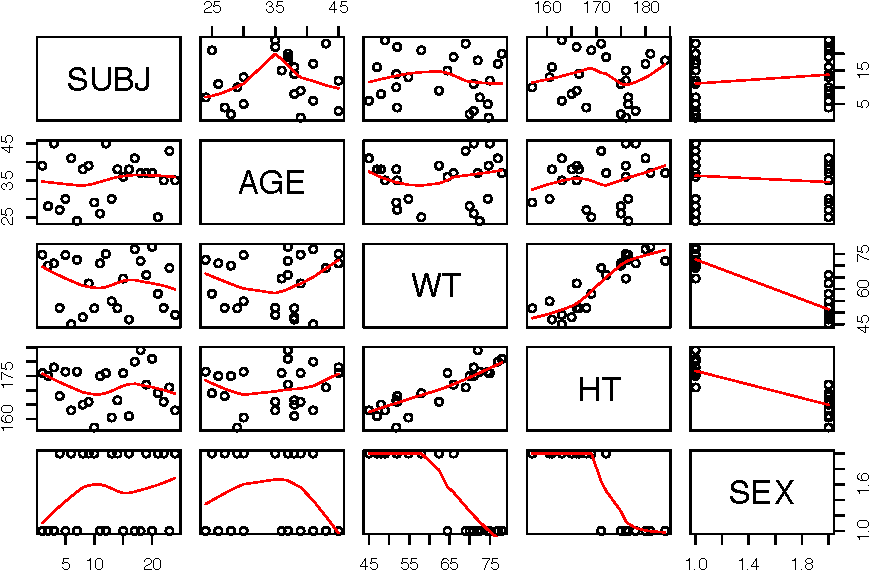
\includegraphics{Rprogramming_files/figure-latex/unnamed-chunk-12-1.pdf}

\begin{Shaded}
\begin{Highlighting}[]
\NormalTok{panel.cor <-}\StringTok{ }\ControlFlowTok{function}\NormalTok{(x, y, }\DataTypeTok{digits=}\DecValTok{2}\NormalTok{, }\DataTypeTok{prefix=}\StringTok{""}\NormalTok{, cex.cor)}
\NormalTok{\{}
\NormalTok{    usr <-}\StringTok{ }\KeywordTok{par}\NormalTok{(}\StringTok{"usr"}\NormalTok{); }\KeywordTok{on.exit}\NormalTok{(}\KeywordTok{par}\NormalTok{(usr))}
    \KeywordTok{par}\NormalTok{(}\DataTypeTok{usr =} \KeywordTok{c}\NormalTok{(}\DecValTok{0}\NormalTok{, }\DecValTok{1}\NormalTok{, }\DecValTok{0}\NormalTok{, }\DecValTok{1}\NormalTok{))}
\NormalTok{    r =}\StringTok{ }\NormalTok{(}\KeywordTok{cor}\NormalTok{(x, y))}
\NormalTok{    txt <-}\StringTok{ }\KeywordTok{format}\NormalTok{(}\KeywordTok{c}\NormalTok{(r, }\FloatTok{0.123456789}\NormalTok{), }\DataTypeTok{digits=}\NormalTok{digits)[}\DecValTok{1}\NormalTok{]}
\NormalTok{    txt <-}\StringTok{ }\KeywordTok{paste}\NormalTok{(prefix, txt, }\DataTypeTok{sep=}\StringTok{""}\NormalTok{)}
    \ControlFlowTok{if}\NormalTok{(}\KeywordTok{missing}\NormalTok{(cex.cor)) cex <-}\StringTok{ }\FloatTok{1.5}
    \KeywordTok{text}\NormalTok{(}\FloatTok{0.5}\NormalTok{, }\FloatTok{0.5}\NormalTok{, txt, }\DataTypeTok{cex =} \FloatTok{1.5}\NormalTok{)}
\NormalTok{\}}

\KeywordTok{pairs}\NormalTok{(d.demog, }\DataTypeTok{lower.panel=}\NormalTok{panel.smooth, }\DataTypeTok{upper.panel=}\NormalTok{panel.cor) }
\end{Highlighting}
\end{Shaded}

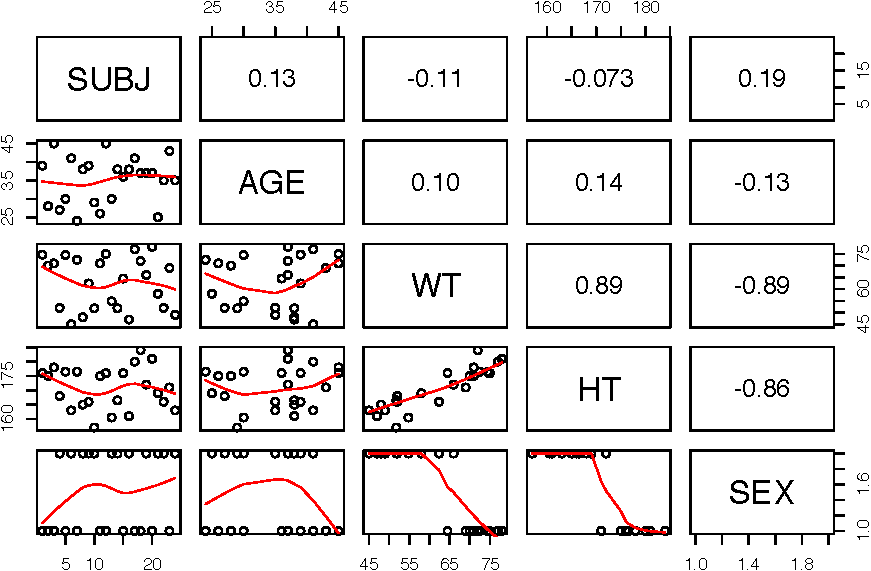
\includegraphics{Rprogramming_files/figure-latex/unnamed-chunk-12-2.pdf}

\section{하위수준 그림 함수}\label{lower}

\begin{itemize}
\tightlist
\item
  points : 점추가
\item
  lines : 선 추가
\item
  abline : 기준선 추가
\item
  mtext : 텍스트 추가
\item
  legend : 설명(legend) 추가
\item
  polygon : polygon 추가
\end{itemize}

\subsection{점, 선, 설명 추가 하기 \{add\}}\label{-----add}

\begin{Shaded}
\begin{Highlighting}[]
\KeywordTok{plot}\NormalTok{(pct.}\DecValTok{95}\OperatorTok{$}\NormalTok{TIME, pct.}\DecValTok{95}\OperatorTok{$}\NormalTok{PCT50, }\DataTypeTok{main=}\StringTok{"PK of Drug X"}
\NormalTok{     , }\DataTypeTok{type=}\StringTok{"l"}\NormalTok{, }\DataTypeTok{xlab=}\StringTok{"Time (h)"}\NormalTok{, }\DataTypeTok{ylab=}\StringTok{"Concentration (ng/ml)"}
\NormalTok{     , }\DataTypeTok{ylim=}\KeywordTok{range}\NormalTok{(}\DecValTok{0}\NormalTok{,}\DecValTok{80}\NormalTok{), }\DataTypeTok{lty=}\DecValTok{1}\NormalTok{, }\DataTypeTok{col=}\StringTok{"red"}\NormalTok{, }\DataTypeTok{lwd=}\DecValTok{2}\NormalTok{)}
\end{Highlighting}
\end{Shaded}

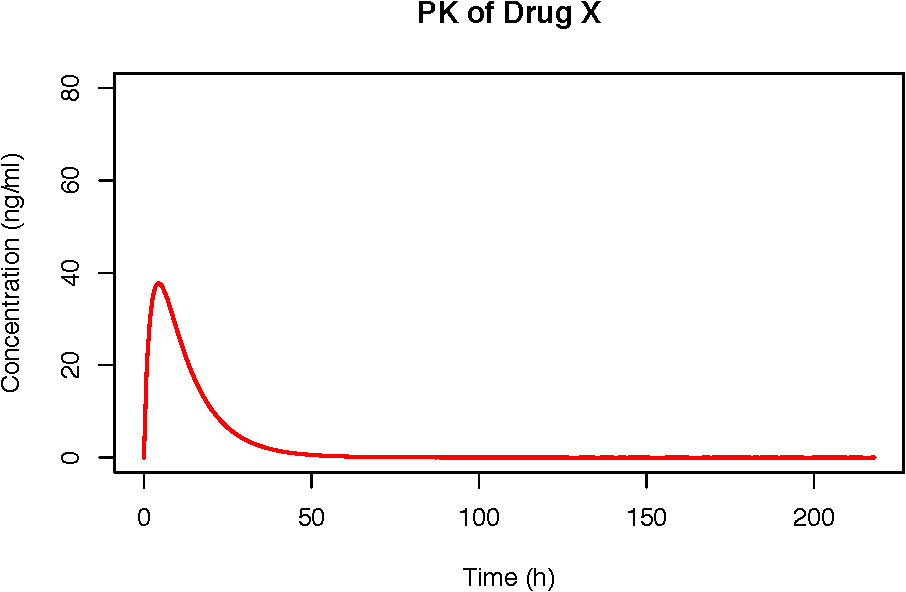
\includegraphics{Rprogramming_files/figure-latex/unnamed-chunk-13-1.pdf}

\begin{Shaded}
\begin{Highlighting}[]
\KeywordTok{plot}\NormalTok{(dta}\OperatorTok{$}\NormalTok{TIME[dta}\OperatorTok{$}\NormalTok{MDV}\OperatorTok{==}\DecValTok{0}\NormalTok{], dta}\OperatorTok{$}\NormalTok{DV[dta}\OperatorTok{$}\NormalTok{MDV}\OperatorTok{==}\DecValTok{0}\NormalTok{], }\DataTypeTok{main=}\StringTok{"PK of Drug X"}
\NormalTok{     , }\DataTypeTok{type=}\StringTok{"n"}\NormalTok{, }\DataTypeTok{xlab=}\StringTok{"Time (h)"}\NormalTok{, }\DataTypeTok{ylab=}\StringTok{"Concentration (ng/ml)"}
\NormalTok{     , }\DataTypeTok{ylim=}\KeywordTok{range}\NormalTok{(}\DecValTok{0}\NormalTok{,}\DecValTok{80}\NormalTok{))}
\KeywordTok{points}\NormalTok{(dta}\OperatorTok{$}\NormalTok{TIME[dta}\OperatorTok{$}\NormalTok{MDV}\OperatorTok{==}\DecValTok{0}\NormalTok{], dta}\OperatorTok{$}\NormalTok{DV[dta}\OperatorTok{$}\NormalTok{MDV}\OperatorTok{==}\DecValTok{0}\NormalTok{], }\DataTypeTok{pch =} \DecValTok{16}\NormalTok{, }\DataTypeTok{cex=}\FloatTok{0.8}\NormalTok{)}
\KeywordTok{lines}\NormalTok{(dta}\OperatorTok{$}\NormalTok{TIME[dta}\OperatorTok{$}\NormalTok{MDV}\OperatorTok{==}\DecValTok{0}\NormalTok{], dta}\OperatorTok{$}\NormalTok{DV[dta}\OperatorTok{$}\NormalTok{MDV}\OperatorTok{==}\DecValTok{0}\NormalTok{], }\DataTypeTok{col=}\StringTok{"black"}\NormalTok{, }\DataTypeTok{lwd=}\DecValTok{1}\NormalTok{)}
\KeywordTok{abline}\NormalTok{(}\DecValTok{40}\NormalTok{, }\DecValTok{0}\NormalTok{, }\DataTypeTok{col=}\StringTok{"red"}\NormalTok{, }\DataTypeTok{lty=}\DecValTok{2}\NormalTok{)                               }\CommentTok{# abline(a,b): y=a+b*x}
\KeywordTok{legend}\NormalTok{(}\StringTok{"topright"}\NormalTok{, }\DataTypeTok{legend=}\KeywordTok{c}\NormalTok{(}\StringTok{"Individual concentrations"}\NormalTok{)}
\NormalTok{       , }\DataTypeTok{lty=}\DecValTok{1}\NormalTok{, }\DataTypeTok{col=}\StringTok{"black"}\NormalTok{)}
\end{Highlighting}
\end{Shaded}

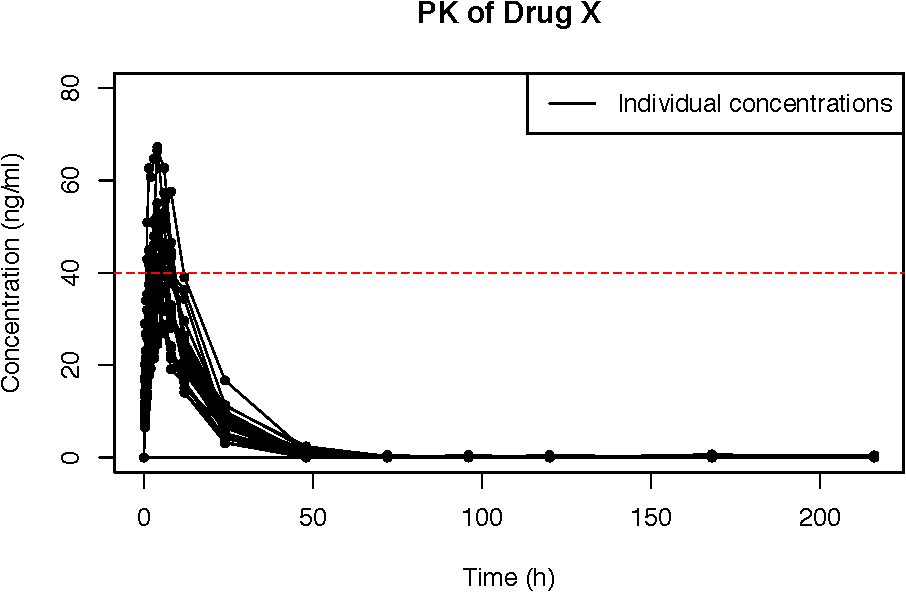
\includegraphics{Rprogramming_files/figure-latex/unnamed-chunk-13-2.pdf}

\subsection{polygon 함수}\label{polygon-}

\begin{Shaded}
\begin{Highlighting}[]
\KeywordTok{plot}\NormalTok{(}\KeywordTok{c}\NormalTok{(}\DecValTok{1}\NormalTok{, }\DecValTok{10}\NormalTok{), }\KeywordTok{c}\NormalTok{(}\DecValTok{1}\NormalTok{, }\DecValTok{6}\NormalTok{), }\DataTypeTok{type =} \StringTok{"n"}\NormalTok{)}
\KeywordTok{polygon}\NormalTok{(}\KeywordTok{c}\NormalTok{(}\DecValTok{2}\NormalTok{,}\DecValTok{8}\NormalTok{,}\DecValTok{8}\NormalTok{,}\DecValTok{2}\NormalTok{), }\KeywordTok{c}\NormalTok{(}\DecValTok{5}\NormalTok{,}\DecValTok{4}\NormalTok{,}\DecValTok{3}\NormalTok{,}\DecValTok{2}\NormalTok{), }\DataTypeTok{col=}\StringTok{"lightgreen"}\NormalTok{)}
\end{Highlighting}
\end{Shaded}

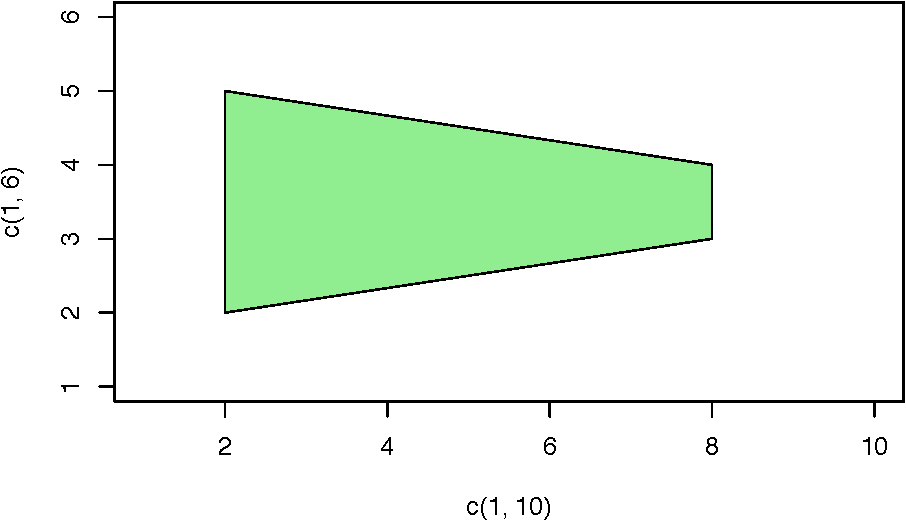
\includegraphics{Rprogramming_files/figure-latex/unnamed-chunk-14-1.pdf}

\begin{Shaded}
\begin{Highlighting}[]
\KeywordTok{plot}\NormalTok{(}\KeywordTok{c}\NormalTok{(}\DecValTok{1}\NormalTok{, }\DecValTok{9}\NormalTok{), }\DecValTok{1}\OperatorTok{:}\DecValTok{2}\NormalTok{, }\DataTypeTok{type =} \StringTok{"n"}\NormalTok{)}
\KeywordTok{polygon}\NormalTok{(}\DecValTok{1}\OperatorTok{:}\DecValTok{9}\NormalTok{, }\KeywordTok{c}\NormalTok{(}\DecValTok{2}\NormalTok{,}\DecValTok{1}\NormalTok{,}\DecValTok{2}\NormalTok{,}\DecValTok{1}\NormalTok{,}\DecValTok{1}\NormalTok{,}\DecValTok{2}\NormalTok{,}\DecValTok{1}\NormalTok{,}\DecValTok{2}\NormalTok{,}\DecValTok{1}\NormalTok{),}
        \DataTypeTok{col =} \KeywordTok{c}\NormalTok{(}\StringTok{"red"}\NormalTok{, }\StringTok{"blue"}\NormalTok{),}
        \DataTypeTok{border =} \KeywordTok{c}\NormalTok{(}\StringTok{"green"}\NormalTok{, }\StringTok{"yellow"}\NormalTok{),}
        \DataTypeTok{lwd =} \DecValTok{3}\NormalTok{, }\DataTypeTok{lty =} \KeywordTok{c}\NormalTok{(}\StringTok{"dashed"}\NormalTok{, }\StringTok{"solid"}\NormalTok{))}
\end{Highlighting}
\end{Shaded}

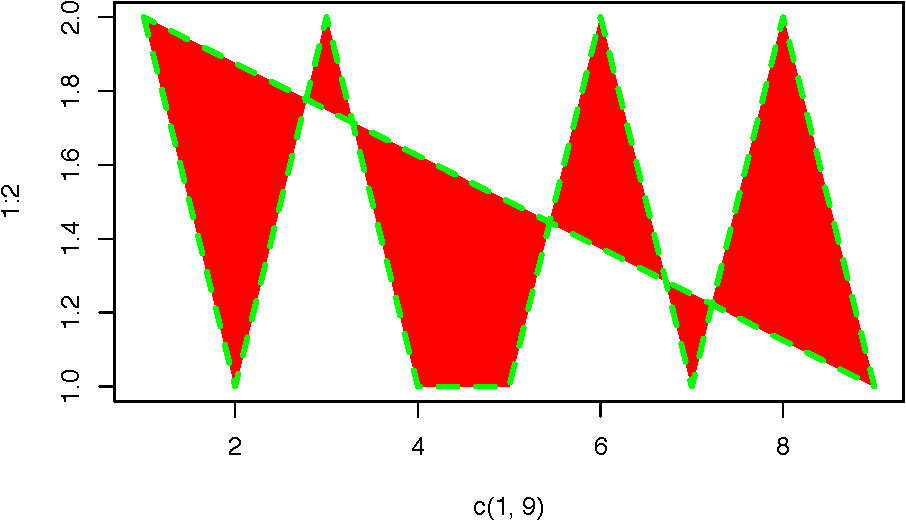
\includegraphics{Rprogramming_files/figure-latex/unnamed-chunk-14-2.pdf}

\section{그림 출력하기}\label{print}

\subsection{pdf graphics devices}\label{pdf-graphics-devices}

\begin{Shaded}
\begin{Highlighting}[]
\KeywordTok{pdf}\NormalTok{(}\StringTok{"PK_of_Drug_X.pdf"}\NormalTok{)}

\KeywordTok{plot}\NormalTok{(dta}\OperatorTok{$}\NormalTok{TIME[dta}\OperatorTok{$}\NormalTok{MDV}\OperatorTok{==}\DecValTok{0}\NormalTok{], dta}\OperatorTok{$}\NormalTok{DV[dta}\OperatorTok{$}\NormalTok{MDV}\OperatorTok{==}\DecValTok{0}\NormalTok{], }\DataTypeTok{main=}\StringTok{"PK of Drug X"}
\NormalTok{     , }\DataTypeTok{type=}\StringTok{"n"}\NormalTok{, }\DataTypeTok{xlab=}\StringTok{"Time (h)"}\NormalTok{, }\DataTypeTok{ylab=}\StringTok{"Concentration (ng/ml)"}
\NormalTok{     , }\DataTypeTok{ylim=}\KeywordTok{range}\NormalTok{(}\DecValTok{0}\NormalTok{,}\DecValTok{80}\NormalTok{))}
\KeywordTok{points}\NormalTok{(dta}\OperatorTok{$}\NormalTok{TIME[dta}\OperatorTok{$}\NormalTok{MDV}\OperatorTok{==}\DecValTok{0}\NormalTok{], dta}\OperatorTok{$}\NormalTok{DV[dta}\OperatorTok{$}\NormalTok{MDV}\OperatorTok{==}\DecValTok{0}\NormalTok{], }\DataTypeTok{pch =} \DecValTok{16}\NormalTok{, }\DataTypeTok{cex=}\FloatTok{0.8}\NormalTok{)}
\KeywordTok{lines}\NormalTok{(dta}\OperatorTok{$}\NormalTok{TIME[dta}\OperatorTok{$}\NormalTok{MDV}\OperatorTok{==}\DecValTok{0}\NormalTok{], dta}\OperatorTok{$}\NormalTok{DV[dta}\OperatorTok{$}\NormalTok{MDV}\OperatorTok{==}\DecValTok{0}\NormalTok{], }\DataTypeTok{col=}\StringTok{"black"}\NormalTok{, }\DataTypeTok{lwd=}\DecValTok{1}\NormalTok{)}
\KeywordTok{abline}\NormalTok{(}\DecValTok{40}\NormalTok{, }\DecValTok{0}\NormalTok{, }\DataTypeTok{col=}\StringTok{"red"}\NormalTok{, }\DataTypeTok{lty=}\DecValTok{2}\NormalTok{)                               }\CommentTok{#abline(a,b): y=a+b*x}
\KeywordTok{legend}\NormalTok{(}\StringTok{"topright"}\NormalTok{, }\DataTypeTok{legend=}\KeywordTok{c}\NormalTok{(}\StringTok{"Individual concentrations"}\NormalTok{)}
\NormalTok{       , }\DataTypeTok{lty=}\DecValTok{1}\NormalTok{, }\DataTypeTok{col=}\StringTok{"black"}\NormalTok{)}

\KeywordTok{dev.off}\NormalTok{()}
\end{Highlighting}
\end{Shaded}

\begin{verbatim}
## cairo_pdf 
##         2
\end{verbatim}

\subsection{PNG graphics devices}\label{png-graphics-devices}

\begin{Shaded}
\begin{Highlighting}[]
\KeywordTok{png}\NormalTok{(}\StringTok{"PK_of_Drug_X.png"}\NormalTok{)}

\KeywordTok{plot}\NormalTok{(dta}\OperatorTok{$}\NormalTok{TIME[dta}\OperatorTok{$}\NormalTok{MDV}\OperatorTok{==}\DecValTok{0}\NormalTok{], dta}\OperatorTok{$}\NormalTok{DV[dta}\OperatorTok{$}\NormalTok{MDV}\OperatorTok{==}\DecValTok{0}\NormalTok{], }\DataTypeTok{main=}\StringTok{"PK of Drug X"}
\NormalTok{     , }\DataTypeTok{type=}\StringTok{"n"}\NormalTok{, }\DataTypeTok{xlab=}\StringTok{"Time (h)"}\NormalTok{, }\DataTypeTok{ylab=}\StringTok{"Concentration (ng/ml)"}
\NormalTok{     , }\DataTypeTok{ylim=}\KeywordTok{range}\NormalTok{(}\DecValTok{0}\NormalTok{,}\DecValTok{80}\NormalTok{))}
\KeywordTok{points}\NormalTok{(dta}\OperatorTok{$}\NormalTok{TIME[dta}\OperatorTok{$}\NormalTok{MDV}\OperatorTok{==}\DecValTok{0}\NormalTok{], dta}\OperatorTok{$}\NormalTok{DV[dta}\OperatorTok{$}\NormalTok{MDV}\OperatorTok{==}\DecValTok{0}\NormalTok{], }\DataTypeTok{pch =} \DecValTok{16}\NormalTok{, }\DataTypeTok{cex=}\FloatTok{0.8}\NormalTok{)}
\KeywordTok{lines}\NormalTok{(dta}\OperatorTok{$}\NormalTok{TIME[dta}\OperatorTok{$}\NormalTok{MDV}\OperatorTok{==}\DecValTok{0}\NormalTok{], dta}\OperatorTok{$}\NormalTok{DV[dta}\OperatorTok{$}\NormalTok{MDV}\OperatorTok{==}\DecValTok{0}\NormalTok{], }\DataTypeTok{col=}\StringTok{"black"}\NormalTok{, }\DataTypeTok{lwd=}\DecValTok{1}\NormalTok{)}
\KeywordTok{abline}\NormalTok{(}\DecValTok{40}\NormalTok{, }\DecValTok{0}\NormalTok{, }\DataTypeTok{col=}\StringTok{"red"}\NormalTok{, }\DataTypeTok{lty=}\DecValTok{2}\NormalTok{)                               }\CommentTok{#abline(a,b): y=a+b*x}
\KeywordTok{legend}\NormalTok{(}\StringTok{"topright"}\NormalTok{, }\DataTypeTok{legend=}\KeywordTok{c}\NormalTok{(}\StringTok{"Individual concentrations"}\NormalTok{)}
\NormalTok{       , }\DataTypeTok{lty=}\DecValTok{1}\NormalTok{, }\DataTypeTok{col=}\StringTok{"black"}\NormalTok{)}

\KeywordTok{dev.off}\NormalTok{()}
\end{Highlighting}
\end{Shaded}

\begin{verbatim}
## cairo_pdf 
##         2
\end{verbatim}

\chapter{Data Import / Export}\label{data-import-export}

\begin{quote}
2017-03-29 배균섭 교수님 강의
\end{quote}

이번 시간에는 자료를 불러오고 조작을 가한 뒤 저장하는 방법에 대해
알아보겠습니다.

\section{Read.csv}\label{read.csv}

\texttt{setwd} 명령어를 통해서 자료가 있는 작업 공간을 설정할 수
있습니다. 설정 후에서는 \texttt{dir()}을 통해 파일의 이름을 확인 할 수
있습니다. \texttt{read.csv}를 통해서 자료를 R에서 사용할 수 있게 됩니다.

\begin{Shaded}
\begin{Highlighting}[]
\KeywordTok{setwd}\NormalTok{(}\StringTok{"D:/Rt"}\NormalTok{)}
\KeywordTok{dir}\NormalTok{()}
\NormalTok{mydata <-}\StringTok{ }\KeywordTok{read.csv}\NormalTok{(}\StringTok{"MyData2017.csv"}\NormalTok{, }\DataTypeTok{as.is=}\OtherTok{TRUE}\NormalTok{)}
\end{Highlighting}
\end{Shaded}

\section{Theoph 데이타}\label{theoph-}

R에 기본적으로 들어있는 \texttt{Theoph} 약동학 자료에 대해
살펴보겠습니다.

\begin{Shaded}
\begin{Highlighting}[]
\KeywordTok{head}\NormalTok{(Theoph, }\DataTypeTok{n =} \DecValTok{11}\NormalTok{)}
\end{Highlighting}
\end{Shaded}

\begin{verbatim}
##    Subject   Wt Dose  Time  conc
## 1        1 79.6 4.02  0.00  0.74
## 2        1 79.6 4.02  0.25  2.84
## 3        1 79.6 4.02  0.57  6.57
## 4        1 79.6 4.02  1.12 10.50
## 5        1 79.6 4.02  2.02  9.66
## 6        1 79.6 4.02  3.82  8.58
## 7        1 79.6 4.02  5.10  8.36
## 8        1 79.6 4.02  7.03  7.47
## 9        1 79.6 4.02  9.05  6.89
## 10       1 79.6 4.02 12.12  5.94
## 11       1 79.6 4.02 24.37  3.28
\end{verbatim}

\begin{Shaded}
\begin{Highlighting}[]
\KeywordTok{tail}\NormalTok{(Theoph, }\DataTypeTok{n =} \DecValTok{11}\NormalTok{)}
\end{Highlighting}
\end{Shaded}

\begin{verbatim}
##     Subject   Wt Dose  Time conc
## 122      12 60.5  5.3  0.00 0.00
## 123      12 60.5  5.3  0.25 1.25
## 124      12 60.5  5.3  0.50 3.96
## 125      12 60.5  5.3  1.00 7.82
## 126      12 60.5  5.3  2.00 9.72
## 127      12 60.5  5.3  3.52 9.75
## 128      12 60.5  5.3  5.07 8.57
## 129      12 60.5  5.3  7.07 6.59
## 130      12 60.5  5.3  9.03 6.11
## 131      12 60.5  5.3 12.05 4.57
## 132      12 60.5  5.3 24.15 1.17
\end{verbatim}

R console에서 \texttt{?Theoph}를 타이핑 치면 좀 더 자세한 정보를 얻을 수
있습니다.

\section{lattice}\label{lattice}

lattice 패키지를 불러온 뒤 그림을 그려보겠습니다. \citep{R-lattice}
\index{lattice}

\begin{Shaded}
\begin{Highlighting}[]
\KeywordTok{library}\NormalTok{(lattice) }\CommentTok{# trellis}

\KeywordTok{xyplot}\NormalTok{(conc }\OperatorTok{~}\StringTok{ }\NormalTok{Time }\OperatorTok{|}\StringTok{ }\NormalTok{Subject, }\DataTypeTok{data=}\NormalTok{Theoph)}
\end{Highlighting}
\end{Shaded}

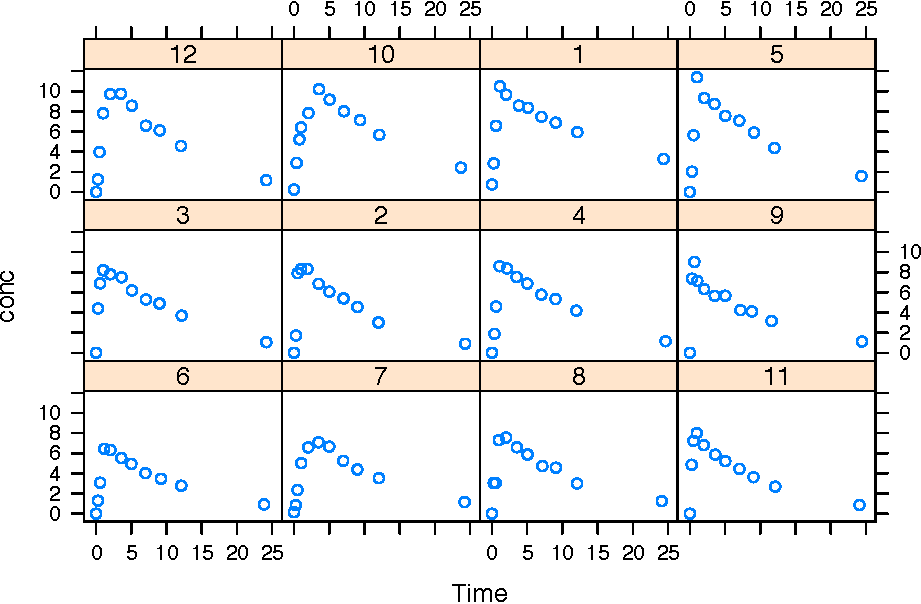
\includegraphics{Rprogramming_files/figure-latex/unnamed-chunk-19-1.pdf}

\begin{Shaded}
\begin{Highlighting}[]
\KeywordTok{xyplot}\NormalTok{(conc }\OperatorTok{~}\StringTok{ }\NormalTok{Time }\OperatorTok{|}\StringTok{ }\NormalTok{Subject, }\DataTypeTok{data=}\NormalTok{Theoph, }\DataTypeTok{type=}\StringTok{"b"}\NormalTok{)}
\end{Highlighting}
\end{Shaded}

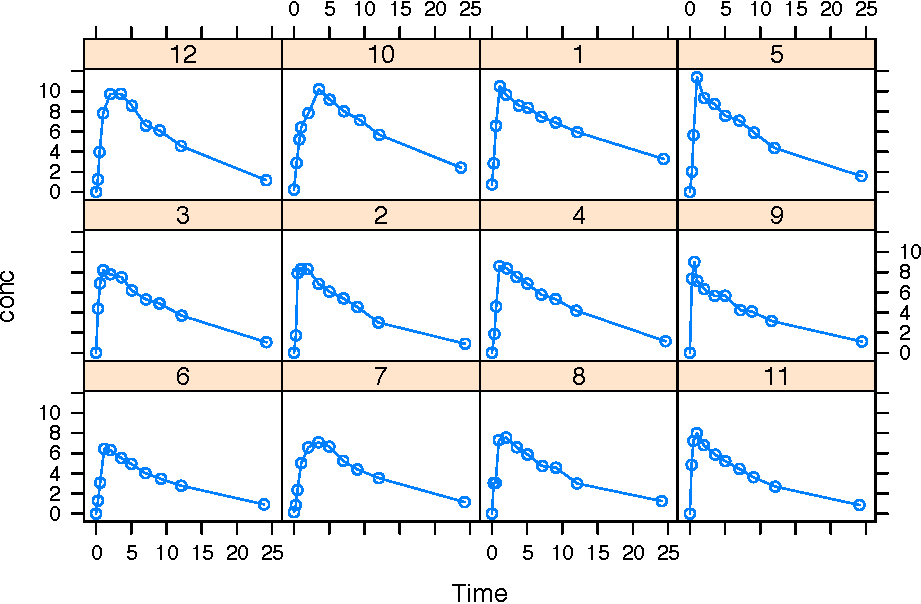
\includegraphics{Rprogramming_files/figure-latex/unnamed-chunk-19-2.pdf}

\begin{Shaded}
\begin{Highlighting}[]
\NormalTok{Theoph[,}\StringTok{"ID"}\NormalTok{] =}\StringTok{ }\KeywordTok{as.numeric}\NormalTok{(}\KeywordTok{as.character}\NormalTok{(Theoph[,}\StringTok{"Subject"}\NormalTok{]))}

\KeywordTok{xyplot}\NormalTok{(conc }\OperatorTok{~}\StringTok{ }\NormalTok{Time }\OperatorTok{|}\StringTok{ }\NormalTok{ID, }\DataTypeTok{data=}\NormalTok{Theoph, }\DataTypeTok{type=}\StringTok{"b"}\NormalTok{)}
\end{Highlighting}
\end{Shaded}

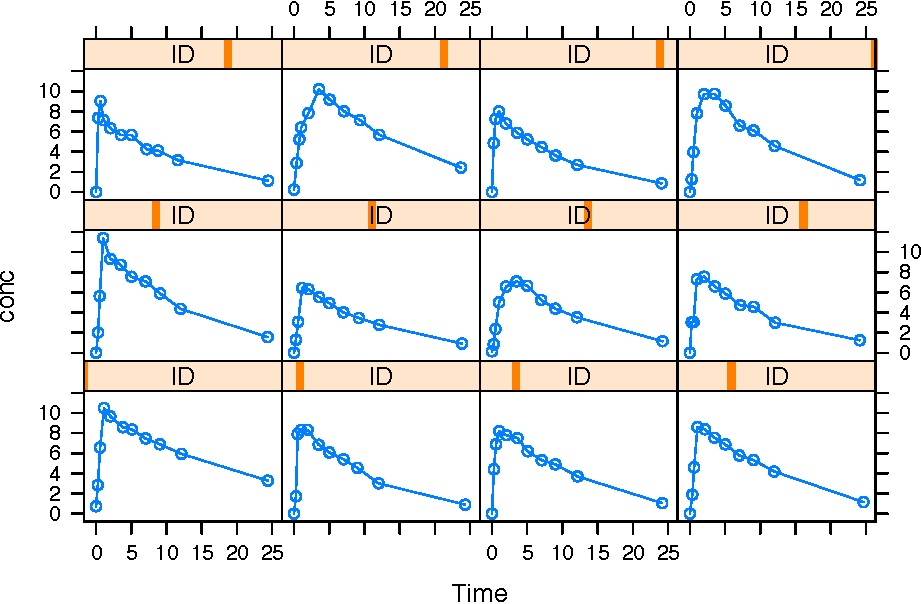
\includegraphics{Rprogramming_files/figure-latex/unnamed-chunk-19-3.pdf}

\begin{Shaded}
\begin{Highlighting}[]
\KeywordTok{xyplot}\NormalTok{(conc }\OperatorTok{~}\StringTok{ }\NormalTok{Time }\OperatorTok{|}\StringTok{ }\KeywordTok{as.factor}\NormalTok{(ID), }\DataTypeTok{data=}\NormalTok{Theoph, }\DataTypeTok{type=}\StringTok{"b"}\NormalTok{)}
\end{Highlighting}
\end{Shaded}

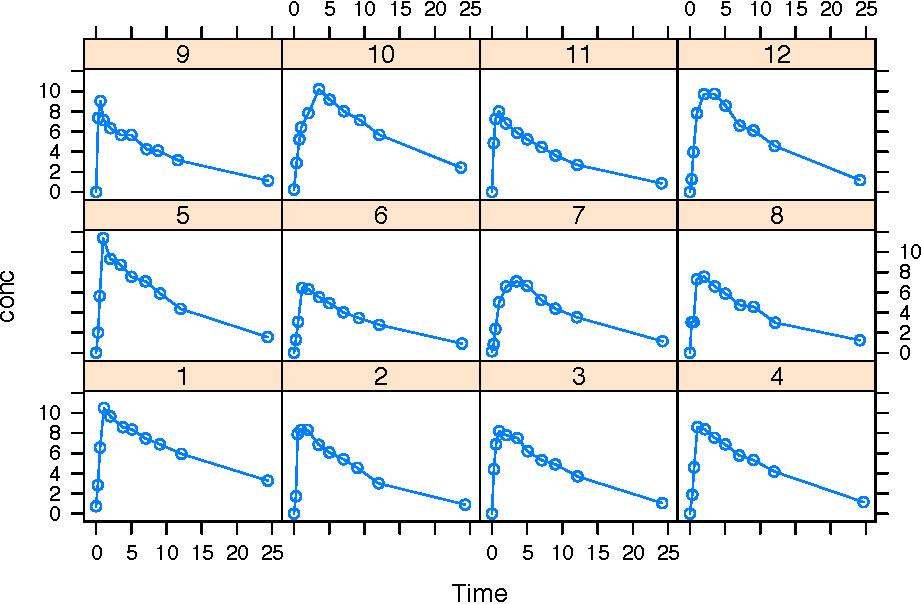
\includegraphics{Rprogramming_files/figure-latex/unnamed-chunk-19-4.pdf}

\begin{Shaded}
\begin{Highlighting}[]
\KeywordTok{write.csv}\NormalTok{(Theoph, }\StringTok{"Theoph.csv"}\NormalTok{, }\DataTypeTok{row.names=}\OtherTok{FALSE}\NormalTok{, }\DataTypeTok{quote=}\OtherTok{FALSE}\NormalTok{, }\DataTypeTok{na=}\StringTok{""}\NormalTok{)}
\end{Highlighting}
\end{Shaded}

\section{Subseting and write.csv}\label{subseting-and-write.csv}

자료를 편집하고, subset을 만들고 각각을 파일로 저장하는 방법에 대해
알아보겠습니다.

\begin{Shaded}
\begin{Highlighting}[]
\NormalTok{IDs =}\StringTok{ }\KeywordTok{sort}\NormalTok{(}\KeywordTok{unique}\NormalTok{(Theoph[,}\StringTok{"ID"}\NormalTok{])) ; IDs}
\end{Highlighting}
\end{Shaded}

\begin{verbatim}
##  [1]  1  2  3  4  5  6  7  8  9 10 11 12
\end{verbatim}

\begin{Shaded}
\begin{Highlighting}[]
\NormalTok{nID =}\StringTok{ }\KeywordTok{length}\NormalTok{(IDs) ; nID}
\end{Highlighting}
\end{Shaded}

\begin{verbatim}
## [1] 12
\end{verbatim}

\begin{Shaded}
\begin{Highlighting}[]
\NormalTok{demog =}\StringTok{ }\KeywordTok{unique}\NormalTok{(Theoph[,}\KeywordTok{c}\NormalTok{(}\StringTok{"ID"}\NormalTok{,}\StringTok{"Wt"}\NormalTok{)])}
\KeywordTok{colnames}\NormalTok{(demog) =}\StringTok{ }\KeywordTok{c}\NormalTok{(}\StringTok{"ID"}\NormalTok{, }\StringTok{"BWT"}\NormalTok{)}
\KeywordTok{write.csv}\NormalTok{(demog, }\StringTok{"1-demog.csv"}\NormalTok{, }\DataTypeTok{row.names=}\OtherTok{FALSE}\NormalTok{, }\DataTypeTok{quote=}\OtherTok{FALSE}\NormalTok{, }\DataTypeTok{na=}\StringTok{""}\NormalTok{)}

\NormalTok{DV =}\StringTok{ }\NormalTok{Theoph[,}\KeywordTok{c}\NormalTok{(}\StringTok{"ID"}\NormalTok{,}\StringTok{"Time"}\NormalTok{, }\StringTok{"conc"}\NormalTok{)]}
\KeywordTok{colnames}\NormalTok{(DV) =}\StringTok{ }\KeywordTok{c}\NormalTok{(}\StringTok{"ID"}\NormalTok{, }\StringTok{"TIME"}\NormalTok{, }\StringTok{"DV"}\NormalTok{)}
\KeywordTok{write.csv}\NormalTok{(DV, }\StringTok{"3-DV.csv"}\NormalTok{, }\DataTypeTok{row.names=}\OtherTok{FALSE}\NormalTok{, }\DataTypeTok{quote=}\OtherTok{FALSE}\NormalTok{, }\DataTypeTok{na=}\StringTok{""}\NormalTok{)}

\NormalTok{adm =}\StringTok{ }\KeywordTok{cbind}\NormalTok{(IDs, }\KeywordTok{rep}\NormalTok{(}\DecValTok{0}\NormalTok{, nID), }\KeywordTok{rep}\NormalTok{(}\DecValTok{320}\NormalTok{, nID))}
\KeywordTok{colnames}\NormalTok{(adm) =}\StringTok{ }\KeywordTok{c}\NormalTok{(}\StringTok{"ID"}\NormalTok{, }\StringTok{"TIME"}\NormalTok{, }\StringTok{"AMT"}\NormalTok{)}
\KeywordTok{write.csv}\NormalTok{(adm, }\StringTok{"2-adm.csv"}\NormalTok{, }\DataTypeTok{row.names=}\OtherTok{FALSE}\NormalTok{, }\DataTypeTok{quote=}\OtherTok{FALSE}\NormalTok{, }\DataTypeTok{na=}\StringTok{""}\NormalTok{)}

\NormalTok{demog =}\StringTok{ }\KeywordTok{read.csv}\NormalTok{(}\StringTok{"1-demog.csv"}\NormalTok{, }\DataTypeTok{as.is=}\OtherTok{TRUE}\NormalTok{)}
\NormalTok{adm =}\StringTok{ }\KeywordTok{read.csv}\NormalTok{(}\StringTok{"2-adm.csv"}\NormalTok{, }\DataTypeTok{as.is=}\OtherTok{TRUE}\NormalTok{)}
\NormalTok{dv =}\StringTok{ }\KeywordTok{read.csv}\NormalTok{(}\StringTok{"3-dv.csv"}\NormalTok{, }\DataTypeTok{as.is=}\OtherTok{TRUE}\NormalTok{)}

\NormalTok{AdmDv =}\StringTok{ }\KeywordTok{merge}\NormalTok{(adm, dv, }\DataTypeTok{by=}\KeywordTok{intersect}\NormalTok{(}\KeywordTok{colnames}\NormalTok{(adm), }\KeywordTok{colnames}\NormalTok{(dv)), }\DataTypeTok{all=}\OtherTok{TRUE}\NormalTok{)}
\NormalTok{AdmDv}
\end{Highlighting}
\end{Shaded}

\begin{verbatim}
##     ID  TIME AMT    DV
## 1    1  0.00 320  0.74
## 2    1  0.25  NA  2.84
## 3    1  0.57  NA  6.57
## 4    1  1.12  NA 10.50
## 5    1  2.02  NA  9.66
## 6    1  3.82  NA  8.58
## 7    1  5.10  NA  8.36
## 8    1  7.03  NA  7.47
## 9    1  9.05  NA  6.89
## 10   1 12.12  NA  5.94
## 11   1 24.37  NA  3.28
## 12   2  0.00 320  0.00
## 13   2  0.27  NA  1.72
## 14   2  0.52  NA  7.91
## 15   2  1.00  NA  8.31
## 16   2  1.92  NA  8.33
## 17   2  3.50  NA  6.85
## 18   2  5.02  NA  6.08
## 19   2  7.03  NA  5.40
## 20   2  9.00  NA  4.55
## 21   2 12.00  NA  3.01
## 22   2 24.30  NA  0.90
## 23   3  0.00 320  0.00
## 24   3  0.27  NA  4.40
## 25   3  0.58  NA  6.90
## 26   3  1.02  NA  8.20
## 27   3  2.02  NA  7.80
## 28   3  3.62  NA  7.50
## 29   3  5.08  NA  6.20
## 30   3  7.07  NA  5.30
## 31   3  9.00  NA  4.90
## 32   3 12.15  NA  3.70
## 33   3 24.17  NA  1.05
## 34   4  0.00 320  0.00
## 35   4  0.35  NA  1.89
## 36   4  0.60  NA  4.60
## 37   4  1.07  NA  8.60
## 38   4  2.13  NA  8.38
## 39   4  3.50  NA  7.54
## 40   4  5.02  NA  6.88
## 41   4  7.02  NA  5.78
## 42   4  9.02  NA  5.33
## 43   4 11.98  NA  4.19
## 44   4 24.65  NA  1.15
## 45   5  0.00 320  0.00
## 46   5  0.30  NA  2.02
## 47   5  0.52  NA  5.63
## 48   5  1.00  NA 11.40
## 49   5  2.02  NA  9.33
## 50   5  3.50  NA  8.74
## 51   5  5.02  NA  7.56
## 52   5  7.02  NA  7.09
## 53   5  9.10  NA  5.90
## 54   5 12.00  NA  4.37
## 55   5 24.35  NA  1.57
## 56   6  0.00 320  0.00
## 57   6  0.27  NA  1.29
## 58   6  0.58  NA  3.08
## 59   6  1.15  NA  6.44
## 60   6  2.03  NA  6.32
## 61   6  3.57  NA  5.53
## 62   6  5.00  NA  4.94
## 63   6  7.00  NA  4.02
## 64   6  9.22  NA  3.46
## 65   6 12.10  NA  2.78
## 66   6 23.85  NA  0.92
## 67   7  0.00 320  0.15
## 68   7  0.25  NA  0.85
## 69   7  0.50  NA  2.35
## 70   7  1.02  NA  5.02
## 71   7  2.02  NA  6.58
## 72   7  3.48  NA  7.09
## 73   7  5.00  NA  6.66
## 74   7  6.98  NA  5.25
## 75   7  9.00  NA  4.39
## 76   7 12.05  NA  3.53
## 77   7 24.22  NA  1.15
## 78   8  0.00 320  0.00
## 79   8  0.25  NA  3.05
## 80   8  0.52  NA  3.05
## 81   8  0.98  NA  7.31
## 82   8  2.02  NA  7.56
## 83   8  3.53  NA  6.59
## 84   8  5.05  NA  5.88
## 85   8  7.15  NA  4.73
## 86   8  9.07  NA  4.57
## 87   8 12.10  NA  3.00
## 88   8 24.12  NA  1.25
## 89   9  0.00 320  0.00
## 90   9  0.30  NA  7.37
## 91   9  0.63  NA  9.03
## 92   9  1.05  NA  7.14
## 93   9  2.02  NA  6.33
## 94   9  3.53  NA  5.66
## 95   9  5.02  NA  5.67
## 96   9  7.17  NA  4.24
## 97   9  8.80  NA  4.11
## 98   9 11.60  NA  3.16
## 99   9 24.43  NA  1.12
## 100 10  0.00 320  0.24
## 101 10  0.37  NA  2.89
## 102 10  0.77  NA  5.22
## 103 10  1.02  NA  6.41
## 104 10  2.05  NA  7.83
## 105 10  3.55  NA 10.21
## 106 10  5.05  NA  9.18
## 107 10  7.08  NA  8.02
## 108 10  9.38  NA  7.14
## 109 10 12.10  NA  5.68
## 110 10 23.70  NA  2.42
## 111 11  0.00 320  0.00
## 112 11  0.25  NA  4.86
## 113 11  0.50  NA  7.24
## 114 11  0.98  NA  8.00
## 115 11  1.98  NA  6.81
## 116 11  3.60  NA  5.87
## 117 11  5.02  NA  5.22
## 118 11  7.03  NA  4.45
## 119 11  9.03  NA  3.62
## 120 11 12.12  NA  2.69
## 121 11 24.08  NA  0.86
## 122 12  0.00 320  0.00
## 123 12  0.25  NA  1.25
## 124 12  0.50  NA  3.96
## 125 12  1.00  NA  7.82
## 126 12  2.00  NA  9.72
## 127 12  3.52  NA  9.75
## 128 12  5.07  NA  8.57
## 129 12  7.07  NA  6.59
## 130 12  9.03  NA  6.11
## 131 12 12.05  NA  4.57
## 132 12 24.15  NA  1.17
\end{verbatim}

자료를 병합(\texttt{merge})해 보겠습니다.

\begin{Shaded}
\begin{Highlighting}[]
\NormalTok{DataAll =}\StringTok{ }\KeywordTok{merge}\NormalTok{(demog, AdmDv, }\DataTypeTok{by=}\KeywordTok{c}\NormalTok{(}\StringTok{"ID"}\NormalTok{), }\DataTypeTok{all=}\OtherTok{TRUE}\NormalTok{)}
\NormalTok{DataAll}
\end{Highlighting}
\end{Shaded}

\begin{verbatim}
##     ID  BWT  TIME AMT    DV
## 1    1 79.6  0.00 320  0.74
## 2    1 79.6  0.25  NA  2.84
## 3    1 79.6  0.57  NA  6.57
## 4    1 79.6  1.12  NA 10.50
## 5    1 79.6  2.02  NA  9.66
## 6    1 79.6  3.82  NA  8.58
## 7    1 79.6  5.10  NA  8.36
## 8    1 79.6  7.03  NA  7.47
## 9    1 79.6  9.05  NA  6.89
## 10   1 79.6 12.12  NA  5.94
## 11   1 79.6 24.37  NA  3.28
## 12   2 72.4  0.00 320  0.00
## 13   2 72.4  0.27  NA  1.72
## 14   2 72.4  0.52  NA  7.91
## 15   2 72.4  1.00  NA  8.31
## 16   2 72.4  1.92  NA  8.33
## 17   2 72.4  3.50  NA  6.85
## 18   2 72.4  5.02  NA  6.08
## 19   2 72.4  7.03  NA  5.40
## 20   2 72.4  9.00  NA  4.55
## 21   2 72.4 12.00  NA  3.01
## 22   2 72.4 24.30  NA  0.90
## 23   3 70.5  0.00 320  0.00
## 24   3 70.5  0.27  NA  4.40
## 25   3 70.5  0.58  NA  6.90
## 26   3 70.5  1.02  NA  8.20
## 27   3 70.5  2.02  NA  7.80
## 28   3 70.5  3.62  NA  7.50
## 29   3 70.5  5.08  NA  6.20
## 30   3 70.5  7.07  NA  5.30
## 31   3 70.5  9.00  NA  4.90
## 32   3 70.5 12.15  NA  3.70
## 33   3 70.5 24.17  NA  1.05
## 34   4 72.7  0.00 320  0.00
## 35   4 72.7  0.35  NA  1.89
## 36   4 72.7  0.60  NA  4.60
## 37   4 72.7  1.07  NA  8.60
## 38   4 72.7  2.13  NA  8.38
## 39   4 72.7  3.50  NA  7.54
## 40   4 72.7  5.02  NA  6.88
## 41   4 72.7  7.02  NA  5.78
## 42   4 72.7  9.02  NA  5.33
## 43   4 72.7 11.98  NA  4.19
## 44   4 72.7 24.65  NA  1.15
## 45   5 54.6  0.00 320  0.00
## 46   5 54.6  0.30  NA  2.02
## 47   5 54.6  0.52  NA  5.63
## 48   5 54.6  1.00  NA 11.40
## 49   5 54.6  2.02  NA  9.33
## 50   5 54.6  3.50  NA  8.74
## 51   5 54.6  5.02  NA  7.56
## 52   5 54.6  7.02  NA  7.09
## 53   5 54.6  9.10  NA  5.90
## 54   5 54.6 12.00  NA  4.37
## 55   5 54.6 24.35  NA  1.57
## 56   6 80.0  0.00 320  0.00
## 57   6 80.0  0.27  NA  1.29
## 58   6 80.0  0.58  NA  3.08
## 59   6 80.0  1.15  NA  6.44
## 60   6 80.0  2.03  NA  6.32
## 61   6 80.0  3.57  NA  5.53
## 62   6 80.0  5.00  NA  4.94
## 63   6 80.0  7.00  NA  4.02
## 64   6 80.0  9.22  NA  3.46
## 65   6 80.0 12.10  NA  2.78
## 66   6 80.0 23.85  NA  0.92
## 67   7 64.6  0.00 320  0.15
## 68   7 64.6  0.25  NA  0.85
## 69   7 64.6  0.50  NA  2.35
## 70   7 64.6  1.02  NA  5.02
## 71   7 64.6  2.02  NA  6.58
## 72   7 64.6  3.48  NA  7.09
## 73   7 64.6  5.00  NA  6.66
## 74   7 64.6  6.98  NA  5.25
## 75   7 64.6  9.00  NA  4.39
## 76   7 64.6 12.05  NA  3.53
## 77   7 64.6 24.22  NA  1.15
## 78   8 70.5  0.00 320  0.00
## 79   8 70.5  0.25  NA  3.05
## 80   8 70.5  0.52  NA  3.05
## 81   8 70.5  0.98  NA  7.31
## 82   8 70.5  2.02  NA  7.56
## 83   8 70.5  3.53  NA  6.59
## 84   8 70.5  5.05  NA  5.88
## 85   8 70.5  7.15  NA  4.73
## 86   8 70.5  9.07  NA  4.57
## 87   8 70.5 12.10  NA  3.00
## 88   8 70.5 24.12  NA  1.25
## 89   9 86.4  0.00 320  0.00
## 90   9 86.4  0.30  NA  7.37
## 91   9 86.4  0.63  NA  9.03
## 92   9 86.4  1.05  NA  7.14
## 93   9 86.4  2.02  NA  6.33
## 94   9 86.4  3.53  NA  5.66
## 95   9 86.4  5.02  NA  5.67
## 96   9 86.4  7.17  NA  4.24
## 97   9 86.4  8.80  NA  4.11
## 98   9 86.4 11.60  NA  3.16
## 99   9 86.4 24.43  NA  1.12
## 100 10 58.2  0.00 320  0.24
## 101 10 58.2  0.37  NA  2.89
## 102 10 58.2  0.77  NA  5.22
## 103 10 58.2  1.02  NA  6.41
## 104 10 58.2  2.05  NA  7.83
## 105 10 58.2  3.55  NA 10.21
## 106 10 58.2  5.05  NA  9.18
## 107 10 58.2  7.08  NA  8.02
## 108 10 58.2  9.38  NA  7.14
## 109 10 58.2 12.10  NA  5.68
## 110 10 58.2 23.70  NA  2.42
## 111 11 65.0  0.00 320  0.00
## 112 11 65.0  0.25  NA  4.86
## 113 11 65.0  0.50  NA  7.24
## 114 11 65.0  0.98  NA  8.00
## 115 11 65.0  1.98  NA  6.81
## 116 11 65.0  3.60  NA  5.87
## 117 11 65.0  5.02  NA  5.22
## 118 11 65.0  7.03  NA  4.45
## 119 11 65.0  9.03  NA  3.62
## 120 11 65.0 12.12  NA  2.69
## 121 11 65.0 24.08  NA  0.86
## 122 12 60.5  0.00 320  0.00
## 123 12 60.5  0.25  NA  1.25
## 124 12 60.5  0.50  NA  3.96
## 125 12 60.5  1.00  NA  7.82
## 126 12 60.5  2.00  NA  9.72
## 127 12 60.5  3.52  NA  9.75
## 128 12 60.5  5.07  NA  8.57
## 129 12 60.5  7.07  NA  6.59
## 130 12 60.5  9.03  NA  6.11
## 131 12 60.5 12.05  NA  4.57
## 132 12 60.5 24.15  NA  1.17
\end{verbatim}

\chapter{Frequently Used Functions}\label{frequently-used-functions}

\begin{quote}
2017-04-05 배균섭 교수님 강의
\end{quote}

자주 쓰는 함수 및 명령어에 대해 알아보겠습니다.

\section{Command}\label{command}

\begin{Shaded}
\begin{Highlighting}[]
\CommentTok{# 2017-04-05 R-intro.pdf Chapter 08}

\NormalTok{pois}
\end{Highlighting}
\end{Shaded}

\begin{verbatim}
## Error in eval(expr, envir, enclos): 객체 'pois'를 찾을 수 없습니다
\end{verbatim}

\begin{Shaded}
\begin{Highlighting}[]
\CommentTok{# ?dbeta}
\KeywordTok{dnorm}\NormalTok{(}\DecValTok{0}\NormalTok{)}
\end{Highlighting}
\end{Shaded}

\begin{verbatim}
## [1] 0.3989
\end{verbatim}

\begin{Shaded}
\begin{Highlighting}[]
\KeywordTok{pnorm}\NormalTok{(}\DecValTok{0}\NormalTok{)}
\end{Highlighting}
\end{Shaded}

\begin{verbatim}
## [1] 0.5
\end{verbatim}

\begin{Shaded}
\begin{Highlighting}[]
\DecValTok{1} \OperatorTok{-}\StringTok{ }\KeywordTok{pnorm}\NormalTok{(}\FloatTok{1.96}\NormalTok{)}
\end{Highlighting}
\end{Shaded}

\begin{verbatim}
## [1] 0.025
\end{verbatim}

\begin{Shaded}
\begin{Highlighting}[]
\CommentTok{# ?pnorm}
\KeywordTok{pnorm}\NormalTok{(}\FloatTok{1.96}\NormalTok{, }\DataTypeTok{lower.tail=}\OtherTok{FALSE}\NormalTok{)}
\end{Highlighting}
\end{Shaded}

\begin{verbatim}
## [1] 0.025
\end{verbatim}

\begin{Shaded}
\begin{Highlighting}[]
\KeywordTok{qnorm}\NormalTok{(}\FloatTok{0.5}\NormalTok{)}
\end{Highlighting}
\end{Shaded}

\begin{verbatim}
## [1] 0
\end{verbatim}

\begin{Shaded}
\begin{Highlighting}[]
\KeywordTok{qnorm}\NormalTok{(}\FloatTok{0.975}\NormalTok{)}
\end{Highlighting}
\end{Shaded}

\begin{verbatim}
## [1] 1.96
\end{verbatim}

\begin{Shaded}
\begin{Highlighting}[]
\KeywordTok{format}\NormalTok{(}\KeywordTok{qnorm}\NormalTok{(}\FloatTok{0.975}\NormalTok{), }\DataTypeTok{digits=}\DecValTok{22}\NormalTok{)}
\end{Highlighting}
\end{Shaded}

\begin{verbatim}
## [1] "1.959963984540053605343"
\end{verbatim}

\begin{Shaded}
\begin{Highlighting}[]
\KeywordTok{rnorm}\NormalTok{(}\DecValTok{5}\NormalTok{)}
\end{Highlighting}
\end{Shaded}

\begin{verbatim}
## [1] -1.0995  0.3497  0.4523  0.9362 -0.3453
\end{verbatim}

\begin{Shaded}
\begin{Highlighting}[]
\KeywordTok{rnorm}\NormalTok{(}\DecValTok{5}\NormalTok{, }\DecValTok{10}\NormalTok{, }\DecValTok{1}\NormalTok{)}
\end{Highlighting}
\end{Shaded}

\begin{verbatim}
## [1] 10.01 10.78 10.29  9.76 10.42
\end{verbatim}

\begin{Shaded}
\begin{Highlighting}[]
\NormalTok{x =}\StringTok{ }\KeywordTok{rnorm}\NormalTok{(}\DecValTok{100}\NormalTok{, }\DecValTok{10}\NormalTok{, }\DecValTok{1}\NormalTok{)}
\KeywordTok{mean}\NormalTok{(x)}
\end{Highlighting}
\end{Shaded}

\begin{verbatim}
## [1] 10.13
\end{verbatim}

\begin{Shaded}
\begin{Highlighting}[]
\KeywordTok{sd}\NormalTok{(x)}
\end{Highlighting}
\end{Shaded}

\begin{verbatim}
## [1] 0.9674
\end{verbatim}

\begin{Shaded}
\begin{Highlighting}[]
\DecValTok{2}\OperatorTok{*}\KeywordTok{pt}\NormalTok{(}\OperatorTok{-}\FloatTok{2.43}\NormalTok{, }\DataTypeTok{df =} \DecValTok{13}\NormalTok{)}
\end{Highlighting}
\end{Shaded}

\begin{verbatim}
## [1] 0.03033
\end{verbatim}

\begin{Shaded}
\begin{Highlighting}[]
\DecValTok{2}\OperatorTok{*}\KeywordTok{pt}\NormalTok{(}\OperatorTok{-}\FloatTok{2.43}\NormalTok{, }\DataTypeTok{df =} \DecValTok{1000}\NormalTok{)}
\end{Highlighting}
\end{Shaded}

\begin{verbatim}
## [1] 0.01527
\end{verbatim}

\begin{Shaded}
\begin{Highlighting}[]
\KeywordTok{qnorm}\NormalTok{(}\FloatTok{0.995}\NormalTok{)}
\end{Highlighting}
\end{Shaded}

\begin{verbatim}
## [1] 2.576
\end{verbatim}

\begin{Shaded}
\begin{Highlighting}[]
\KeywordTok{qf}\NormalTok{(}\FloatTok{0.01}\NormalTok{, }\DecValTok{2}\NormalTok{, }\DecValTok{7}\NormalTok{, }\DataTypeTok{lower.tail =} \OtherTok{FALSE}\NormalTok{)}
\end{Highlighting}
\end{Shaded}

\begin{verbatim}
## [1] 9.547
\end{verbatim}

\begin{Shaded}
\begin{Highlighting}[]
\CommentTok{# ?fivenum}
\NormalTok{faithful}
\end{Highlighting}
\end{Shaded}

\begin{verbatim}
##     eruptions waiting
## 1       3.600      79
## 2       1.800      54
## 3       3.333      74
## 4       2.283      62
## 5       4.533      85
## 6       2.883      55
## 7       4.700      88
## 8       3.600      85
## 9       1.950      51
## 10      4.350      85
## 11      1.833      54
## 12      3.917      84
## 13      4.200      78
## 14      1.750      47
## 15      4.700      83
## 16      2.167      52
## 17      1.750      62
## 18      4.800      84
## 19      1.600      52
## 20      4.250      79
## 21      1.800      51
## 22      1.750      47
## 23      3.450      78
## 24      3.067      69
## 25      4.533      74
## 26      3.600      83
## 27      1.967      55
## 28      4.083      76
## 29      3.850      78
## 30      4.433      79
## 31      4.300      73
## 32      4.467      77
## 33      3.367      66
## 34      4.033      80
## 35      3.833      74
## 36      2.017      52
## 37      1.867      48
## 38      4.833      80
## 39      1.833      59
## 40      4.783      90
## 41      4.350      80
## 42      1.883      58
## 43      4.567      84
## 44      1.750      58
## 45      4.533      73
## 46      3.317      83
## 47      3.833      64
## 48      2.100      53
## 49      4.633      82
## 50      2.000      59
## 51      4.800      75
## 52      4.716      90
## 53      1.833      54
## 54      4.833      80
## 55      1.733      54
## 56      4.883      83
## 57      3.717      71
## 58      1.667      64
## 59      4.567      77
## 60      4.317      81
## 61      2.233      59
## 62      4.500      84
## 63      1.750      48
## 64      4.800      82
## 65      1.817      60
## 66      4.400      92
## 67      4.167      78
## 68      4.700      78
## 69      2.067      65
## 70      4.700      73
## 71      4.033      82
## 72      1.967      56
## 73      4.500      79
## 74      4.000      71
## 75      1.983      62
## 76      5.067      76
## 77      2.017      60
## 78      4.567      78
## 79      3.883      76
## 80      3.600      83
## 81      4.133      75
## 82      4.333      82
## 83      4.100      70
## 84      2.633      65
## 85      4.067      73
## 86      4.933      88
## 87      3.950      76
## 88      4.517      80
## 89      2.167      48
## 90      4.000      86
## 91      2.200      60
## 92      4.333      90
## 93      1.867      50
## 94      4.817      78
## 95      1.833      63
## 96      4.300      72
## 97      4.667      84
## 98      3.750      75
## 99      1.867      51
## 100     4.900      82
## 101     2.483      62
## 102     4.367      88
## 103     2.100      49
## 104     4.500      83
## 105     4.050      81
## 106     1.867      47
## 107     4.700      84
## 108     1.783      52
## 109     4.850      86
## 110     3.683      81
## 111     4.733      75
## 112     2.300      59
## 113     4.900      89
## 114     4.417      79
## 115     1.700      59
## 116     4.633      81
## 117     2.317      50
## 118     4.600      85
## 119     1.817      59
## 120     4.417      87
## 121     2.617      53
## 122     4.067      69
## 123     4.250      77
## 124     1.967      56
## 125     4.600      88
## 126     3.767      81
## 127     1.917      45
## 128     4.500      82
## 129     2.267      55
## 130     4.650      90
## 131     1.867      45
## 132     4.167      83
## 133     2.800      56
## 134     4.333      89
## 135     1.833      46
## 136     4.383      82
## 137     1.883      51
## 138     4.933      86
## 139     2.033      53
## 140     3.733      79
## 141     4.233      81
## 142     2.233      60
## 143     4.533      82
## 144     4.817      77
## 145     4.333      76
## 146     1.983      59
## 147     4.633      80
## 148     2.017      49
## 149     5.100      96
## 150     1.800      53
## 151     5.033      77
## 152     4.000      77
## 153     2.400      65
## 154     4.600      81
## 155     3.567      71
## 156     4.000      70
## 157     4.500      81
## 158     4.083      93
## 159     1.800      53
## 160     3.967      89
## 161     2.200      45
## 162     4.150      86
## 163     2.000      58
## 164     3.833      78
## 165     3.500      66
## 166     4.583      76
## 167     2.367      63
## 168     5.000      88
## 169     1.933      52
## 170     4.617      93
## 171     1.917      49
## 172     2.083      57
## 173     4.583      77
## 174     3.333      68
## 175     4.167      81
## 176     4.333      81
## 177     4.500      73
## 178     2.417      50
## 179     4.000      85
## 180     4.167      74
## 181     1.883      55
## 182     4.583      77
## 183     4.250      83
## 184     3.767      83
## 185     2.033      51
## 186     4.433      78
## 187     4.083      84
## 188     1.833      46
## 189     4.417      83
## 190     2.183      55
## 191     4.800      81
## 192     1.833      57
## 193     4.800      76
## 194     4.100      84
## 195     3.966      77
## 196     4.233      81
## 197     3.500      87
## 198     4.366      77
## 199     2.250      51
## 200     4.667      78
## 201     2.100      60
## 202     4.350      82
## 203     4.133      91
## 204     1.867      53
## 205     4.600      78
## 206     1.783      46
## 207     4.367      77
## 208     3.850      84
## 209     1.933      49
## 210     4.500      83
## 211     2.383      71
## 212     4.700      80
## 213     1.867      49
## 214     3.833      75
## 215     3.417      64
## 216     4.233      76
## 217     2.400      53
## 218     4.800      94
## 219     2.000      55
## 220     4.150      76
## 221     1.867      50
## 222     4.267      82
## 223     1.750      54
## 224     4.483      75
## 225     4.000      78
## 226     4.117      79
## 227     4.083      78
## 228     4.267      78
## 229     3.917      70
## 230     4.550      79
## 231     4.083      70
## 232     2.417      54
## 233     4.183      86
## 234     2.217      50
## 235     4.450      90
## 236     1.883      54
## 237     1.850      54
## 238     4.283      77
## 239     3.950      79
## 240     2.333      64
## 241     4.150      75
## 242     2.350      47
## 243     4.933      86
## 244     2.900      63
## 245     4.583      85
## 246     3.833      82
## 247     2.083      57
## 248     4.367      82
## 249     2.133      67
## 250     4.350      74
## 251     2.200      54
## 252     4.450      83
## 253     3.567      73
## 254     4.500      73
## 255     4.150      88
## 256     3.817      80
## 257     3.917      71
## 258     4.450      83
## 259     2.000      56
## 260     4.283      79
## 261     4.767      78
## 262     4.533      84
## 263     1.850      58
## 264     4.250      83
## 265     1.983      43
## 266     2.250      60
## 267     4.750      75
## 268     4.117      81
## 269     2.150      46
## 270     4.417      90
## 271     1.817      46
## 272     4.467      74
\end{verbatim}

\begin{Shaded}
\begin{Highlighting}[]
\KeywordTok{str}\NormalTok{(faithful)}
\end{Highlighting}
\end{Shaded}

\begin{verbatim}
## 'data.frame':    272 obs. of  2 variables:
##  $ eruptions: num  3.6 1.8 3.33 2.28 4.53 ...
##  $ waiting  : num  79 54 74 62 85 55 88 85 51 85 ...
\end{verbatim}

\begin{Shaded}
\begin{Highlighting}[]
\NormalTok{eruptions}
\end{Highlighting}
\end{Shaded}

\begin{verbatim}
## Error in eval(expr, envir, enclos): 객체 'eruptions'를 찾을 수 없습니다
\end{verbatim}

\begin{Shaded}
\begin{Highlighting}[]
\KeywordTok{attach}\NormalTok{(faithful)}
\NormalTok{eruptions}
\end{Highlighting}
\end{Shaded}

\begin{verbatim}
##   [1] 3.600 1.800 3.333 2.283 4.533 2.883 4.700 3.600
##   [9] 1.950 4.350 1.833 3.917 4.200 1.750 4.700 2.167
##  [17] 1.750 4.800 1.600 4.250 1.800 1.750 3.450 3.067
##  [25] 4.533 3.600 1.967 4.083 3.850 4.433 4.300 4.467
##  [33] 3.367 4.033 3.833 2.017 1.867 4.833 1.833 4.783
##  [41] 4.350 1.883 4.567 1.750 4.533 3.317 3.833 2.100
##  [49] 4.633 2.000 4.800 4.716 1.833 4.833 1.733 4.883
##  [57] 3.717 1.667 4.567 4.317 2.233 4.500 1.750 4.800
##  [65] 1.817 4.400 4.167 4.700 2.067 4.700 4.033 1.967
##  [73] 4.500 4.000 1.983 5.067 2.017 4.567 3.883 3.600
##  [81] 4.133 4.333 4.100 2.633 4.067 4.933 3.950 4.517
##  [89] 2.167 4.000 2.200 4.333 1.867 4.817 1.833 4.300
##  [97] 4.667 3.750 1.867 4.900 2.483 4.367 2.100 4.500
## [105] 4.050 1.867 4.700 1.783 4.850 3.683 4.733 2.300
## [113] 4.900 4.417 1.700 4.633 2.317 4.600 1.817 4.417
## [121] 2.617 4.067 4.250 1.967 4.600 3.767 1.917 4.500
## [129] 2.267 4.650 1.867 4.167 2.800 4.333 1.833 4.383
## [137] 1.883 4.933 2.033 3.733 4.233 2.233 4.533 4.817
## [145] 4.333 1.983 4.633 2.017 5.100 1.800 5.033 4.000
## [153] 2.400 4.600 3.567 4.000 4.500 4.083 1.800 3.967
## [161] 2.200 4.150 2.000 3.833 3.500 4.583 2.367 5.000
## [169] 1.933 4.617 1.917 2.083 4.583 3.333 4.167 4.333
## [177] 4.500 2.417 4.000 4.167 1.883 4.583 4.250 3.767
## [185] 2.033 4.433 4.083 1.833 4.417 2.183 4.800 1.833
## [193] 4.800 4.100 3.966 4.233 3.500 4.366 2.250 4.667
## [201] 2.100 4.350 4.133 1.867 4.600 1.783 4.367 3.850
## [209] 1.933 4.500 2.383 4.700 1.867 3.833 3.417 4.233
## [217] 2.400 4.800 2.000 4.150 1.867 4.267 1.750 4.483
## [225] 4.000 4.117 4.083 4.267 3.917 4.550 4.083 2.417
## [233] 4.183 2.217 4.450 1.883 1.850 4.283 3.950 2.333
## [241] 4.150 2.350 4.933 2.900 4.583 3.833 2.083 4.367
## [249] 2.133 4.350 2.200 4.450 3.567 4.500 4.150 3.817
## [257] 3.917 4.450 2.000 4.283 4.767 4.533 1.850 4.250
## [265] 1.983 2.250 4.750 4.117 2.150 4.417 1.817 4.467
\end{verbatim}

\begin{Shaded}
\begin{Highlighting}[]
\NormalTok{waiting}
\end{Highlighting}
\end{Shaded}

\begin{verbatim}
##   [1] 79 54 74 62 85 55 88 85 51 85 54 84 78 47 83 52
##  [17] 62 84 52 79 51 47 78 69 74 83 55 76 78 79 73 77
##  [33] 66 80 74 52 48 80 59 90 80 58 84 58 73 83 64 53
##  [49] 82 59 75 90 54 80 54 83 71 64 77 81 59 84 48 82
##  [65] 60 92 78 78 65 73 82 56 79 71 62 76 60 78 76 83
##  [81] 75 82 70 65 73 88 76 80 48 86 60 90 50 78 63 72
##  [97] 84 75 51 82 62 88 49 83 81 47 84 52 86 81 75 59
## [113] 89 79 59 81 50 85 59 87 53 69 77 56 88 81 45 82
## [129] 55 90 45 83 56 89 46 82 51 86 53 79 81 60 82 77
## [145] 76 59 80 49 96 53 77 77 65 81 71 70 81 93 53 89
## [161] 45 86 58 78 66 76 63 88 52 93 49 57 77 68 81 81
## [177] 73 50 85 74 55 77 83 83 51 78 84 46 83 55 81 57
## [193] 76 84 77 81 87 77 51 78 60 82 91 53 78 46 77 84
## [209] 49 83 71 80 49 75 64 76 53 94 55 76 50 82 54 75
## [225] 78 79 78 78 70 79 70 54 86 50 90 54 54 77 79 64
## [241] 75 47 86 63 85 82 57 82 67 74 54 83 73 73 88 80
## [257] 71 83 56 79 78 84 58 83 43 60 75 81 46 90 46 74
\end{verbatim}

\begin{Shaded}
\begin{Highlighting}[]
\KeywordTok{stem}\NormalTok{(waiting)}
\end{Highlighting}
\end{Shaded}

\begin{verbatim}
## 
##   The decimal point is 1 digit(s) to the right of the |
## 
##   4 | 3
##   4 | 55566666777788899999
##   5 | 00000111111222223333333444444444
##   5 | 555555666677788889999999
##   6 | 00000022223334444
##   6 | 555667899
##   7 | 00001111123333333444444
##   7 | 555555556666666667777777777778888888888888889999999999
##   8 | 000000001111111111111222222222222333333333333334444444444
##   8 | 55555566666677888888999
##   9 | 00000012334
##   9 | 6
\end{verbatim}

\begin{Shaded}
\begin{Highlighting}[]
\KeywordTok{sort}\NormalTok{(eruptions)}
\end{Highlighting}
\end{Shaded}

\begin{verbatim}
##   [1] 1.600 1.667 1.700 1.733 1.750 1.750 1.750 1.750
##   [9] 1.750 1.750 1.783 1.783 1.800 1.800 1.800 1.800
##  [17] 1.817 1.817 1.817 1.833 1.833 1.833 1.833 1.833
##  [25] 1.833 1.833 1.850 1.850 1.867 1.867 1.867 1.867
##  [33] 1.867 1.867 1.867 1.867 1.883 1.883 1.883 1.883
##  [41] 1.917 1.917 1.933 1.933 1.950 1.967 1.967 1.967
##  [49] 1.983 1.983 1.983 2.000 2.000 2.000 2.000 2.017
##  [57] 2.017 2.017 2.033 2.033 2.067 2.083 2.083 2.100
##  [65] 2.100 2.100 2.133 2.150 2.167 2.167 2.183 2.200
##  [73] 2.200 2.200 2.217 2.233 2.233 2.250 2.250 2.267
##  [81] 2.283 2.300 2.317 2.333 2.350 2.367 2.383 2.400
##  [89] 2.400 2.417 2.417 2.483 2.617 2.633 2.800 2.883
##  [97] 2.900 3.067 3.317 3.333 3.333 3.367 3.417 3.450
## [105] 3.500 3.500 3.567 3.567 3.600 3.600 3.600 3.600
## [113] 3.683 3.717 3.733 3.750 3.767 3.767 3.817 3.833
## [121] 3.833 3.833 3.833 3.833 3.850 3.850 3.883 3.917
## [129] 3.917 3.917 3.950 3.950 3.966 3.967 4.000 4.000
## [137] 4.000 4.000 4.000 4.000 4.033 4.033 4.050 4.067
## [145] 4.067 4.083 4.083 4.083 4.083 4.083 4.100 4.100
## [153] 4.117 4.117 4.133 4.133 4.150 4.150 4.150 4.150
## [161] 4.167 4.167 4.167 4.167 4.183 4.200 4.233 4.233
## [169] 4.233 4.250 4.250 4.250 4.250 4.267 4.267 4.283
## [177] 4.283 4.300 4.300 4.317 4.333 4.333 4.333 4.333
## [185] 4.333 4.350 4.350 4.350 4.350 4.366 4.367 4.367
## [193] 4.367 4.383 4.400 4.417 4.417 4.417 4.417 4.433
## [201] 4.433 4.450 4.450 4.450 4.467 4.467 4.483 4.500
## [209] 4.500 4.500 4.500 4.500 4.500 4.500 4.500 4.517
## [217] 4.533 4.533 4.533 4.533 4.533 4.550 4.567 4.567
## [225] 4.567 4.583 4.583 4.583 4.583 4.600 4.600 4.600
## [233] 4.600 4.617 4.633 4.633 4.633 4.650 4.667 4.667
## [241] 4.700 4.700 4.700 4.700 4.700 4.700 4.716 4.733
## [249] 4.750 4.767 4.783 4.800 4.800 4.800 4.800 4.800
## [257] 4.800 4.817 4.817 4.833 4.833 4.850 4.883 4.900
## [265] 4.900 4.933 4.933 4.933 5.000 5.033 5.067 5.100
\end{verbatim}

\begin{Shaded}
\begin{Highlighting}[]
\KeywordTok{hist}\NormalTok{(eruptions)}
\end{Highlighting}
\end{Shaded}

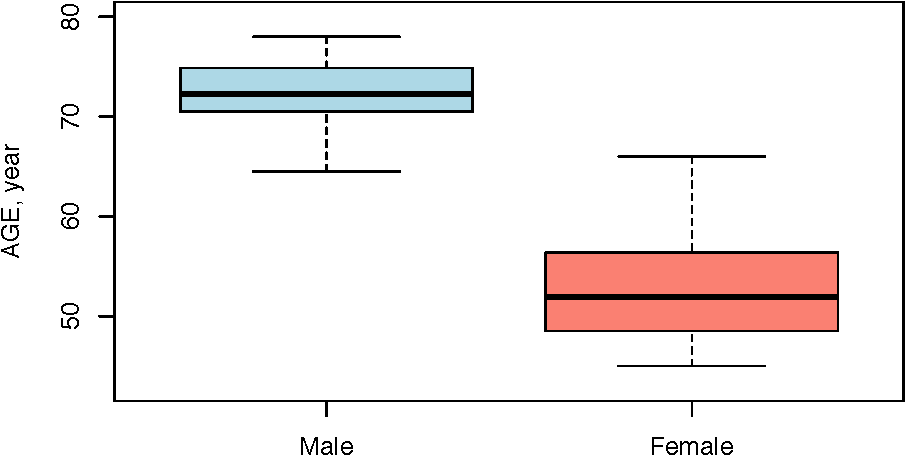
\includegraphics{Rprogramming_files/figure-latex/unnamed-chunk-22-1.pdf}

\begin{Shaded}
\begin{Highlighting}[]
\KeywordTok{hist}\NormalTok{(eruptions, }\KeywordTok{seq}\NormalTok{(}\FloatTok{1.6}\NormalTok{, }\FloatTok{5.2}\NormalTok{, }\FloatTok{0.2}\NormalTok{), }\DataTypeTok{prob=}\OtherTok{TRUE}\NormalTok{)}
\KeywordTok{lines}\NormalTok{(}\KeywordTok{density}\NormalTok{(eruptions, }\DataTypeTok{bw=}\FloatTok{0.1}\NormalTok{))}
\KeywordTok{rug}\NormalTok{(eruptions)}
\CommentTok{# ?hist}
\CommentTok{# ?density}
\KeywordTok{lines}\NormalTok{(}\KeywordTok{density}\NormalTok{(eruptions, }\DataTypeTok{bw=}\StringTok{"SJ"}\NormalTok{), }\DataTypeTok{lty=}\DecValTok{3}\NormalTok{)}
\end{Highlighting}
\end{Shaded}

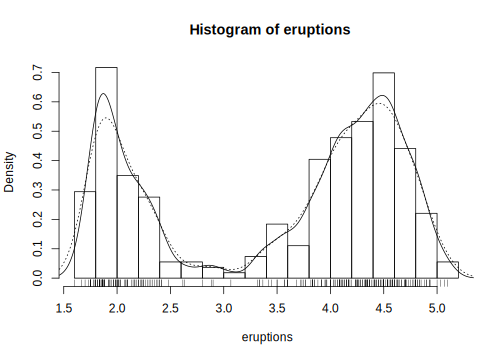
\includegraphics{Rprogramming_files/figure-latex/unnamed-chunk-22-2.pdf}

\begin{Shaded}
\begin{Highlighting}[]
\KeywordTok{plot}\NormalTok{(}\KeywordTok{ecdf}\NormalTok{(eruptions), }\DataTypeTok{do.points=}\OtherTok{FALSE}\NormalTok{, }\DataTypeTok{verticals=}\OtherTok{TRUE}\NormalTok{)}
\end{Highlighting}
\end{Shaded}

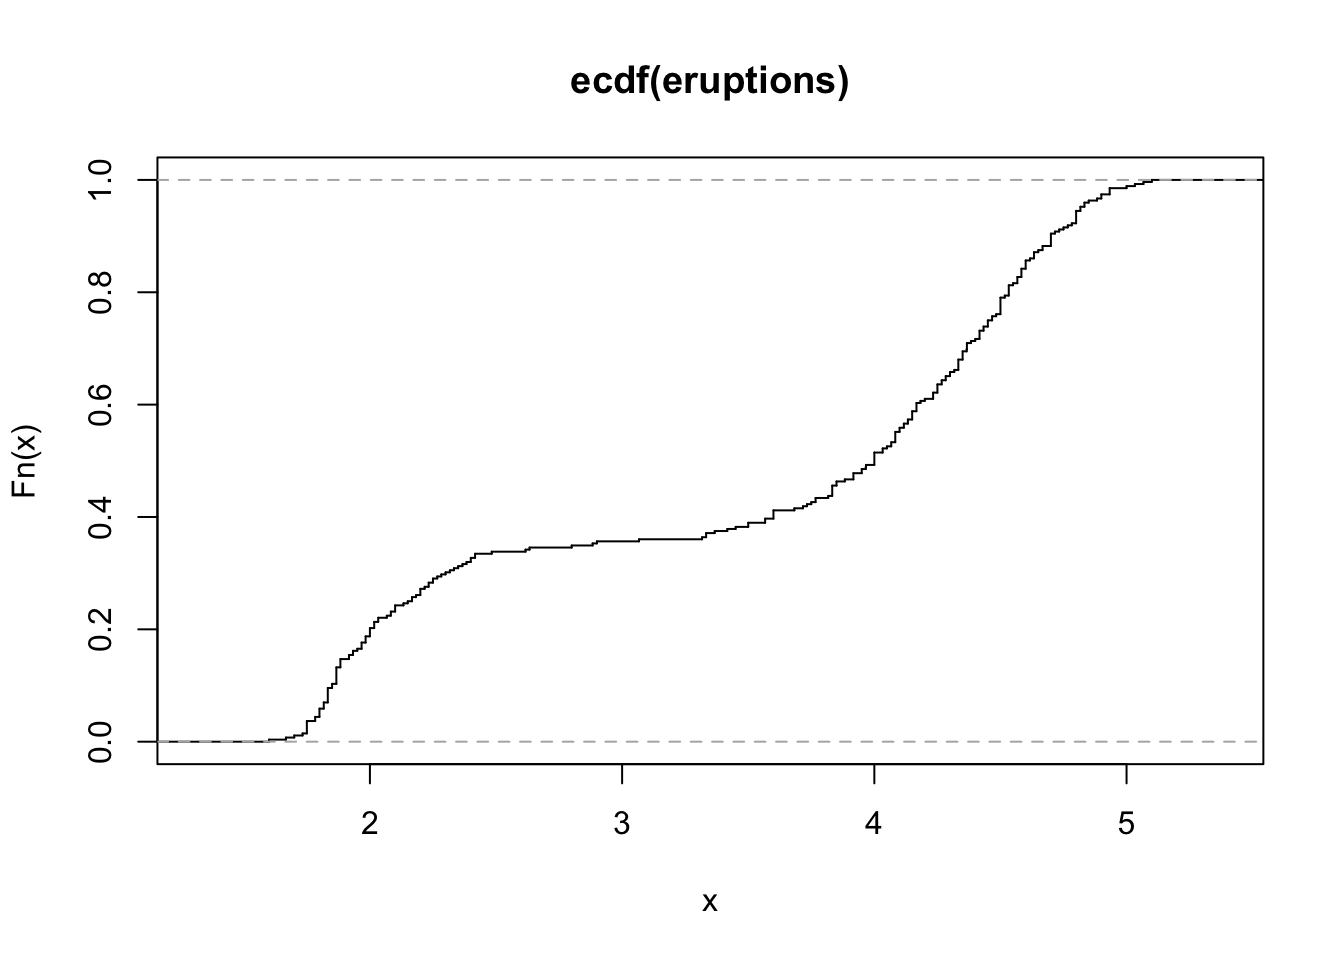
\includegraphics{Rprogramming_files/figure-latex/unnamed-chunk-22-3.pdf}

\begin{Shaded}
\begin{Highlighting}[]
\CommentTok{# ?plot}
\KeywordTok{ecdf}\NormalTok{(eruptions)}
\end{Highlighting}
\end{Shaded}

\begin{verbatim}
## Empirical CDF 
## Call: ecdf(eruptions)
##  x[1:126] = 1.6, 1.7, 1.7,  ..., 5.1, 5.1
\end{verbatim}

\begin{Shaded}
\begin{Highlighting}[]
\NormalTok{x =}\StringTok{ }\KeywordTok{ecdf}\NormalTok{(eruptions)}
\NormalTok{x}
\end{Highlighting}
\end{Shaded}

\begin{verbatim}
## Empirical CDF 
## Call: ecdf(eruptions)
##  x[1:126] = 1.6, 1.7, 1.7,  ..., 5.1, 5.1
\end{verbatim}

\begin{Shaded}
\begin{Highlighting}[]
\KeywordTok{str}\NormalTok{(x)}
\end{Highlighting}
\end{Shaded}

\begin{verbatim}
## function (v)  
##  - attr(*, "class")= chr [1:3] "ecdf" "stepfun" "function"
##  - attr(*, "call")= language ecdf(eruptions)
\end{verbatim}

\begin{Shaded}
\begin{Highlighting}[]
\KeywordTok{x}\NormalTok{()}
\end{Highlighting}
\end{Shaded}

\begin{verbatim}
## Error in .approxfun(x, y, v, method, yleft, yright, f): 기본값이 없는 인수 "v"가 누락되어 있습니다
\end{verbatim}

\begin{Shaded}
\begin{Highlighting}[]
\KeywordTok{plot}\NormalTok{(}\KeywordTok{ecdf}\NormalTok{(eruptions), }\DataTypeTok{do.points=}\OtherTok{FALSE}\NormalTok{)}
\end{Highlighting}
\end{Shaded}

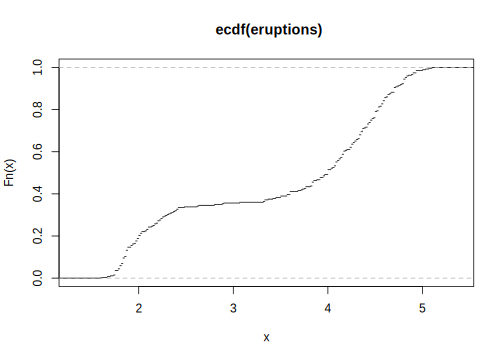
\includegraphics{Rprogramming_files/figure-latex/unnamed-chunk-22-4.pdf}

\begin{Shaded}
\begin{Highlighting}[]
\KeywordTok{plot}\NormalTok{(}\KeywordTok{ecdf}\NormalTok{(eruptions))}
\end{Highlighting}
\end{Shaded}

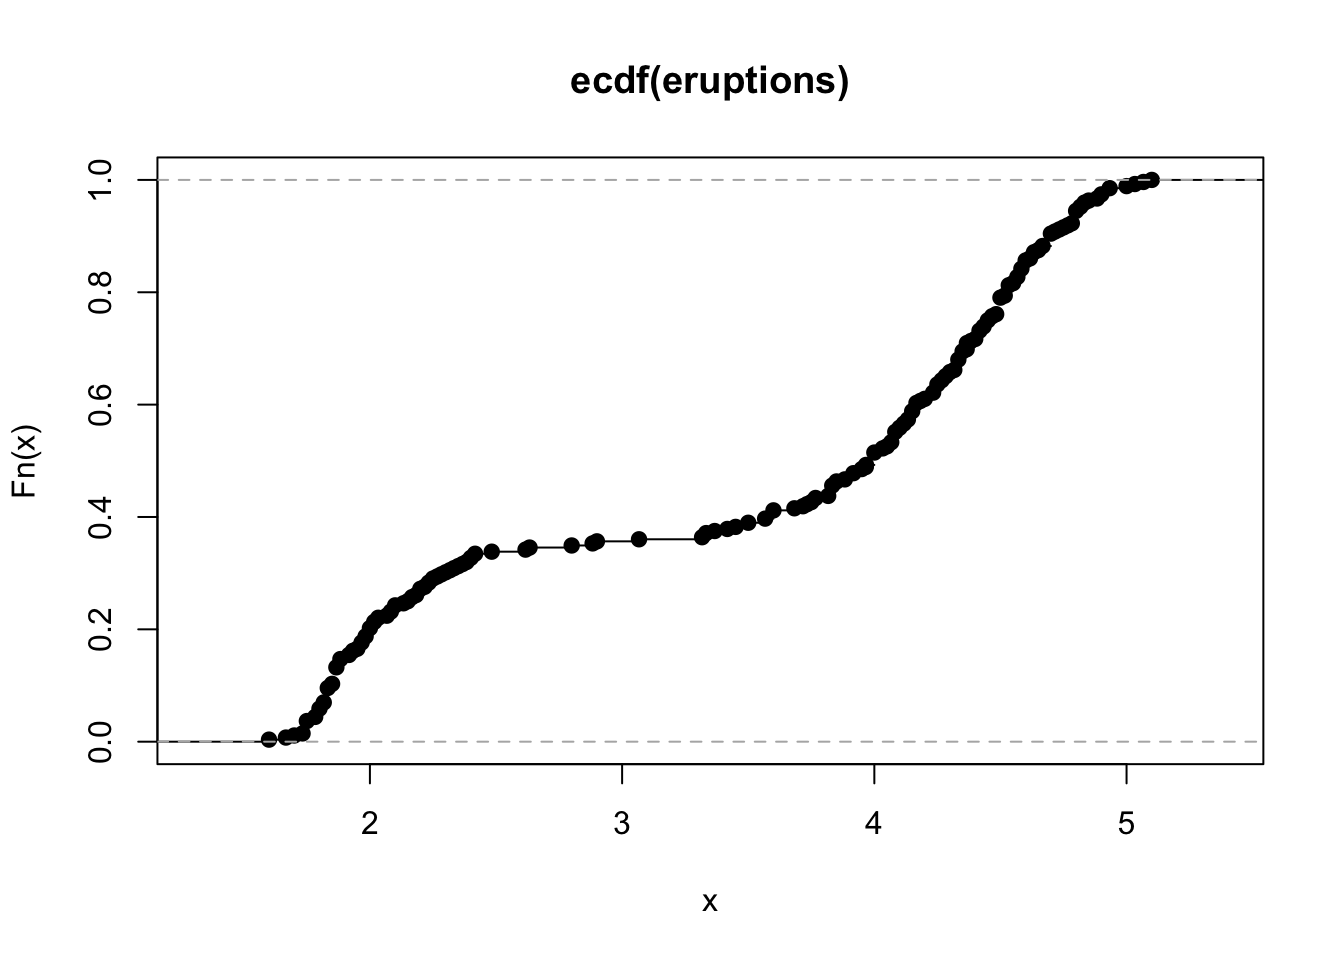
\includegraphics{Rprogramming_files/figure-latex/unnamed-chunk-22-5.pdf}

\begin{Shaded}
\begin{Highlighting}[]
\NormalTok{long <-}\StringTok{ }\NormalTok{eruptions[eruptions }\OperatorTok{>}\StringTok{ }\DecValTok{3}\NormalTok{]}
\NormalTok{x <-}\StringTok{ }\KeywordTok{seq}\NormalTok{(}\DecValTok{3}\NormalTok{, }\FloatTok{5.4}\NormalTok{, }\FloatTok{0.01}\NormalTok{)}
\KeywordTok{pnorm}\NormalTok{(x, }\DataTypeTok{mean=}\KeywordTok{mean}\NormalTok{(long), }\DataTypeTok{sd=}\KeywordTok{sqrt}\NormalTok{(}\KeywordTok{var}\NormalTok{(long)))}
\end{Highlighting}
\end{Shaded}

\begin{verbatim}
##   [1] 0.0008362 0.0009084 0.0009864 0.0010704 0.0011610
##   [6] 0.0012585 0.0013635 0.0014764 0.0015978 0.0017282
##  [11] 0.0018682 0.0020185 0.0021797 0.0023524 0.0025375
##  [16] 0.0027356 0.0029476 0.0031743 0.0034165 0.0036752
##  [21] 0.0039514 0.0042460 0.0045601 0.0048947 0.0052511
##  [26] 0.0056304 0.0060338 0.0064627 0.0069183 0.0074020
##  [31] 0.0079152 0.0084596 0.0090365 0.0096475 0.0102944
##  [36] 0.0109788 0.0117024 0.0124670 0.0132746 0.0141269
##  [41] 0.0150260 0.0159739 0.0169725 0.0180241 0.0191306
##  [46] 0.0202945 0.0215177 0.0228028 0.0241519 0.0255674
##  [51] 0.0270518 0.0286074 0.0302366 0.0319421 0.0337262
##  [56] 0.0355915 0.0375406 0.0395759 0.0417001 0.0439157
##  [61] 0.0462253 0.0486315 0.0511367 0.0537436 0.0564547
##  [66] 0.0592723 0.0621991 0.0652374 0.0683897 0.0716581
##  [71] 0.0750451 0.0785529 0.0821835 0.0859391 0.0898217
##  [76] 0.0938331 0.0979753 0.1022500 0.1066587 0.1112030
##  [81] 0.1158842 0.1207037 0.1256626 0.1307619 0.1360025
##  [86] 0.1413850 0.1469102 0.1525783 0.1583896 0.1643443
##  [91] 0.1704423 0.1766832 0.1830667 0.1895922 0.1962589
##  [96] 0.2030658 0.2100116 0.2170952 0.2243149 0.2316689
## [101] 0.2391554 0.2467722 0.2545170 0.2623872 0.2703803
## [106] 0.2784932 0.2867229 0.2950662 0.3035195 0.3120794
## [111] 0.3207419 0.3295032 0.3383590 0.3473052 0.3563373
## [116] 0.3654507 0.3746407 0.3839025 0.3932310 0.4026213
## [121] 0.4120681 0.4215661 0.4311100 0.4406943 0.4503134
## [126] 0.4599618 0.4696339 0.4793239 0.4890262 0.4987349
## [131] 0.5084444 0.5181489 0.5278427 0.5375199 0.5471751
## [136] 0.5568024 0.5663963 0.5759512 0.5854617 0.5949224
## [141] 0.6043279 0.6136730 0.6229527 0.6321619 0.6412957
## [146] 0.6503494 0.6593184 0.6681982 0.6769845 0.6856732
## [151] 0.6942601 0.7027416 0.7111139 0.7193735 0.7275172
## [156] 0.7355417 0.7434443 0.7512220 0.7588724 0.7663930
## [161] 0.7737818 0.7810366 0.7881558 0.7951377 0.8019809
## [166] 0.8086842 0.8152465 0.8216671 0.8279453 0.8340805
## [171] 0.8400726 0.8459213 0.8516267 0.8571890 0.8626087
## [176] 0.8678862 0.8730222 0.8780176 0.8828733 0.8875905
## [181] 0.8921703 0.8966142 0.9009236 0.9051002 0.9091456
## [186] 0.9130615 0.9168500 0.9205130 0.9240526 0.9274708
## [191] 0.9307700 0.9339522 0.9370200 0.9399756 0.9428215
## [196] 0.9455601 0.9481939 0.9507254 0.9531571 0.9554916
## [201] 0.9577315 0.9598792 0.9619375 0.9639088 0.9657957
## [206] 0.9676007 0.9693264 0.9709753 0.9725498 0.9740525
## [211] 0.9754857 0.9768519 0.9781534 0.9793926 0.9805717
## [216] 0.9816930 0.9827587 0.9837709 0.9847318 0.9856434
## [221] 0.9865077 0.9873267 0.9881024 0.9888365 0.9895310
## [226] 0.9901874 0.9908077 0.9913933 0.9919460 0.9924672
## [231] 0.9929585 0.9934212 0.9938569 0.9942668 0.9946523
## [236] 0.9950145 0.9953548 0.9956741 0.9959737 0.9962546
## [241] 0.9965177
\end{verbatim}

\begin{Shaded}
\begin{Highlighting}[]
\CommentTok{# ?par}
\NormalTok{x <-}\StringTok{ }\KeywordTok{rt}\NormalTok{(}\DecValTok{250}\NormalTok{, }\DataTypeTok{df =} \DecValTok{5}\NormalTok{)}
\KeywordTok{qqnorm}\NormalTok{(x); }\KeywordTok{qqline}\NormalTok{(x)}
\end{Highlighting}
\end{Shaded}

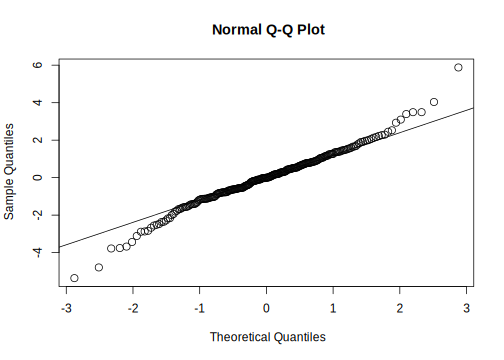
\includegraphics{Rprogramming_files/figure-latex/unnamed-chunk-22-6.pdf}

\begin{Shaded}
\begin{Highlighting}[]
\KeywordTok{curve}\NormalTok{(dnorm, }\OperatorTok{-}\DecValTok{5}\NormalTok{, }\DecValTok{5}\NormalTok{)}
\NormalTok{y =}\StringTok{ }\KeywordTok{density}\NormalTok{(x)}
\KeywordTok{lines}\NormalTok{(y, }\DataTypeTok{lty=}\DecValTok{3}\NormalTok{)}
\end{Highlighting}
\end{Shaded}

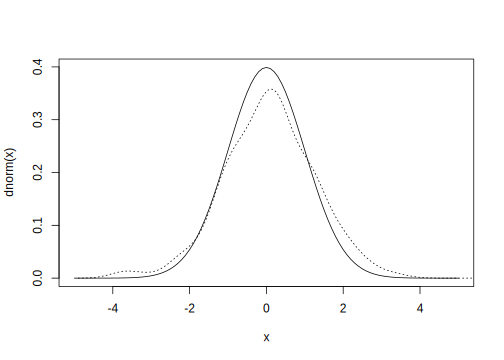
\includegraphics{Rprogramming_files/figure-latex/unnamed-chunk-22-7.pdf}

\begin{Shaded}
\begin{Highlighting}[]
\CommentTok{# ?ppoints}
\KeywordTok{ppoints}\NormalTok{(}\DecValTok{250}\NormalTok{)}
\end{Highlighting}
\end{Shaded}

\begin{verbatim}
##   [1] 0.002 0.006 0.010 0.014 0.018 0.022 0.026 0.030
##   [9] 0.034 0.038 0.042 0.046 0.050 0.054 0.058 0.062
##  [17] 0.066 0.070 0.074 0.078 0.082 0.086 0.090 0.094
##  [25] 0.098 0.102 0.106 0.110 0.114 0.118 0.122 0.126
##  [33] 0.130 0.134 0.138 0.142 0.146 0.150 0.154 0.158
##  [41] 0.162 0.166 0.170 0.174 0.178 0.182 0.186 0.190
##  [49] 0.194 0.198 0.202 0.206 0.210 0.214 0.218 0.222
##  [57] 0.226 0.230 0.234 0.238 0.242 0.246 0.250 0.254
##  [65] 0.258 0.262 0.266 0.270 0.274 0.278 0.282 0.286
##  [73] 0.290 0.294 0.298 0.302 0.306 0.310 0.314 0.318
##  [81] 0.322 0.326 0.330 0.334 0.338 0.342 0.346 0.350
##  [89] 0.354 0.358 0.362 0.366 0.370 0.374 0.378 0.382
##  [97] 0.386 0.390 0.394 0.398 0.402 0.406 0.410 0.414
## [105] 0.418 0.422 0.426 0.430 0.434 0.438 0.442 0.446
## [113] 0.450 0.454 0.458 0.462 0.466 0.470 0.474 0.478
## [121] 0.482 0.486 0.490 0.494 0.498 0.502 0.506 0.510
## [129] 0.514 0.518 0.522 0.526 0.530 0.534 0.538 0.542
## [137] 0.546 0.550 0.554 0.558 0.562 0.566 0.570 0.574
## [145] 0.578 0.582 0.586 0.590 0.594 0.598 0.602 0.606
## [153] 0.610 0.614 0.618 0.622 0.626 0.630 0.634 0.638
## [161] 0.642 0.646 0.650 0.654 0.658 0.662 0.666 0.670
## [169] 0.674 0.678 0.682 0.686 0.690 0.694 0.698 0.702
## [177] 0.706 0.710 0.714 0.718 0.722 0.726 0.730 0.734
## [185] 0.738 0.742 0.746 0.750 0.754 0.758 0.762 0.766
## [193] 0.770 0.774 0.778 0.782 0.786 0.790 0.794 0.798
## [201] 0.802 0.806 0.810 0.814 0.818 0.822 0.826 0.830
## [209] 0.834 0.838 0.842 0.846 0.850 0.854 0.858 0.862
## [217] 0.866 0.870 0.874 0.878 0.882 0.886 0.890 0.894
## [225] 0.898 0.902 0.906 0.910 0.914 0.918 0.922 0.926
## [233] 0.930 0.934 0.938 0.942 0.946 0.950 0.954 0.958
## [241] 0.962 0.966 0.970 0.974 0.978 0.982 0.986 0.990
## [249] 0.994 0.998
\end{verbatim}

\begin{Shaded}
\begin{Highlighting}[]
\KeywordTok{ppoints}\NormalTok{(}\DecValTok{10}\NormalTok{)}
\end{Highlighting}
\end{Shaded}

\begin{verbatim}
##  [1] 0.06098 0.15854 0.25610 0.35366 0.45122 0.54878
##  [7] 0.64634 0.74390 0.84146 0.93902
\end{verbatim}

\begin{Shaded}
\begin{Highlighting}[]
\KeywordTok{qqplot}\NormalTok{(}\KeywordTok{qt}\NormalTok{(}\KeywordTok{ppoints}\NormalTok{(}\DecValTok{250}\NormalTok{), }\DataTypeTok{df =} \DecValTok{5}\NormalTok{), x, }\DataTypeTok{xlab =} \StringTok{"Q-Q plot for t dsn"}\NormalTok{)}
\end{Highlighting}
\end{Shaded}

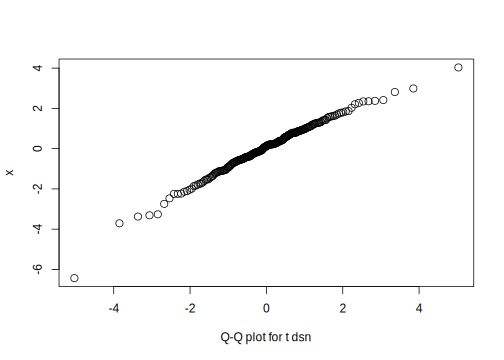
\includegraphics{Rprogramming_files/figure-latex/unnamed-chunk-22-8.pdf}

\begin{Shaded}
\begin{Highlighting}[]
\KeywordTok{windows}\NormalTok{()}
\end{Highlighting}
\end{Shaded}

\begin{verbatim}
## Error in windows(): 함수 "windows"를 찾을 수 없습니다
\end{verbatim}

\begin{Shaded}
\begin{Highlighting}[]
\KeywordTok{qqplot}\NormalTok{(}\KeywordTok{qt}\NormalTok{(}\KeywordTok{runif}\NormalTok{(}\DecValTok{250}\NormalTok{), }\DataTypeTok{df =} \DecValTok{5}\NormalTok{), x, }\DataTypeTok{xlab =} \StringTok{"Q-Q plot for t dsn"}\NormalTok{)}
\end{Highlighting}
\end{Shaded}

\includegraphics{Rprogramming_files/figure-latex/unnamed-chunk-22-9.pdf}

\begin{Shaded}
\begin{Highlighting}[]
\CommentTok{# ?shapiro.test}
\CommentTok{# ?ks.test}
\CommentTok{# ?t.test}


\NormalTok{A =}\StringTok{ }\KeywordTok{c}\NormalTok{(}\FloatTok{79.98}\NormalTok{, }\FloatTok{80.04}\NormalTok{, }\FloatTok{80.02}\NormalTok{, }\FloatTok{80.04}\NormalTok{, }\FloatTok{80.03}\NormalTok{, }\FloatTok{80.03}\NormalTok{, }\FloatTok{80.04}\NormalTok{, }\FloatTok{79.97}\NormalTok{, }\FloatTok{80.05}\NormalTok{, }\FloatTok{80.03}\NormalTok{, }\FloatTok{80.02}\NormalTok{, }\FloatTok{80.00}\NormalTok{, }\FloatTok{80.02}\NormalTok{)}
\NormalTok{B =}\StringTok{ }\KeywordTok{c}\NormalTok{(}\FloatTok{80.02}\NormalTok{, }\FloatTok{79.94}\NormalTok{, }\FloatTok{79.98}\NormalTok{, }\FloatTok{79.97}\NormalTok{, }\FloatTok{79.97}\NormalTok{, }\FloatTok{80.03}\NormalTok{, }\FloatTok{79.95}\NormalTok{, }\FloatTok{79.97}\NormalTok{)}
\KeywordTok{boxplot}\NormalTok{(A, B)}
\end{Highlighting}
\end{Shaded}

\includegraphics{Rprogramming_files/figure-latex/unnamed-chunk-22-10.pdf}

\begin{Shaded}
\begin{Highlighting}[]
\KeywordTok{t.test}\NormalTok{(A, B)}
\end{Highlighting}
\end{Shaded}

\begin{verbatim}
## 
##  Welch Two Sample t-test
## 
## data:  A and B
## t = 3.2, df = 12, p-value = 0.007
## alternative hypothesis: true difference in means is not equal to 0
## 95 percent confidence interval:
##  0.01386 0.07018
## sample estimates:
## mean of x mean of y 
##     80.02     79.98
\end{verbatim}

\begin{Shaded}
\begin{Highlighting}[]
\KeywordTok{var.test}\NormalTok{(A, B)}
\end{Highlighting}
\end{Shaded}

\begin{verbatim}
## 
##  F test to compare two variances
## 
## data:  A and B
## F = 0.58, num df = 12, denom df = 7, p-value =
## 0.4
## alternative hypothesis: true ratio of variances is not equal to 1
## 95 percent confidence interval:
##  0.1251 2.1053
## sample estimates:
## ratio of variances 
##             0.5837
\end{verbatim}

\begin{Shaded}
\begin{Highlighting}[]
\KeywordTok{t.test}\NormalTok{(A, B, }\DataTypeTok{var.equal=}\OtherTok{TRUE}\NormalTok{)}
\end{Highlighting}
\end{Shaded}

\begin{verbatim}
## 
##  Two Sample t-test
## 
## data:  A and B
## t = 3.5, df = 19, p-value = 0.003
## alternative hypothesis: true difference in means is not equal to 0
## 95 percent confidence interval:
##  0.01669 0.06735
## sample estimates:
## mean of x mean of y 
##     80.02     79.98
\end{verbatim}

\begin{Shaded}
\begin{Highlighting}[]
\KeywordTok{wilcox.test}\NormalTok{(A, B)}
\end{Highlighting}
\end{Shaded}

\begin{verbatim}
## Warning in wilcox.test.default(A, B): cannot compute
## exact p-value with ties
\end{verbatim}

\begin{verbatim}
## 
##  Wilcoxon rank sum test with continuity
##  correction
## 
## data:  A and B
## W = 89, p-value = 0.007
## alternative hypothesis: true location shift is not equal to 0
\end{verbatim}

\begin{Shaded}
\begin{Highlighting}[]
\KeywordTok{plot}\NormalTok{(}\KeywordTok{ecdf}\NormalTok{(A), }\DataTypeTok{do.points=}\OtherTok{FALSE}\NormalTok{, }\DataTypeTok{verticals=}\OtherTok{TRUE}\NormalTok{, }\DataTypeTok{xlim=}\KeywordTok{range}\NormalTok{(A, B))}
\KeywordTok{plot}\NormalTok{(}\KeywordTok{ecdf}\NormalTok{(B), }\DataTypeTok{do.points=}\OtherTok{FALSE}\NormalTok{, }\DataTypeTok{verticals=}\OtherTok{TRUE}\NormalTok{, }\DataTypeTok{add=}\OtherTok{TRUE}\NormalTok{)}
\end{Highlighting}
\end{Shaded}

\includegraphics{Rprogramming_files/figure-latex/unnamed-chunk-22-11.pdf}

\begin{Shaded}
\begin{Highlighting}[]
\KeywordTok{ks.test}\NormalTok{(A, B)}
\end{Highlighting}
\end{Shaded}

\begin{verbatim}
## Warning in ks.test(A, B): cannot compute exact p-value
## with ties
\end{verbatim}

\begin{verbatim}
## 
##  Two-sample Kolmogorov-Smirnov test
## 
## data:  A and B
## D = 0.6, p-value = 0.06
## alternative hypothesis: two-sided
\end{verbatim}

\begin{Shaded}
\begin{Highlighting}[]
\CommentTok{# Chapter 9 Grouping, loops and conditional execution}

\CommentTok{# \{ \} does grouping}
\CommentTok{# Usefulness of loops: for >> while >> repeat}
\ControlFlowTok{for}\NormalTok{ (i }\ControlFlowTok{in} \DecValTok{1}\OperatorTok{:}\DecValTok{10}\NormalTok{) \{}
  \KeywordTok{print}\NormalTok{(}\DecValTok{2}\OperatorTok{*}\NormalTok{i)}
\NormalTok{\}}
\end{Highlighting}
\end{Shaded}

\begin{verbatim}
## [1] 2
## [1] 4
## [1] 6
## [1] 8
## [1] 10
## [1] 12
## [1] 14
## [1] 16
## [1] 18
## [1] 20
\end{verbatim}

\begin{Shaded}
\begin{Highlighting}[]
\ControlFlowTok{for}\NormalTok{ (i }\ControlFlowTok{in} \DecValTok{1}\OperatorTok{:}\DecValTok{10}\NormalTok{) }\KeywordTok{print}\NormalTok{(}\DecValTok{2}\OperatorTok{*}\NormalTok{i)}
\end{Highlighting}
\end{Shaded}

\begin{verbatim}
## [1] 2
## [1] 4
## [1] 6
## [1] 8
## [1] 10
## [1] 12
## [1] 14
## [1] 16
## [1] 18
## [1] 20
\end{verbatim}

\begin{Shaded}
\begin{Highlighting}[]
\CommentTok{#while (    ) \{}
\NormalTok{## Statements}
\CommentTok{#\}}

\CommentTok{# # if ~ else ~}
\CommentTok{# if (   ) \{}
\CommentTok{# # Statements 1}
\CommentTok{# \} else \{}
\CommentTok{# # Statements 2}
\CommentTok{# \}}
\CommentTok{# }
\CommentTok{# if (    ) # Statement1}
\CommentTok{# else # Statement2}
\CommentTok{# }
\CommentTok{# if (   ) \{}
\CommentTok{# # Statements 1}
\CommentTok{# \} else if (   ) \{}
\CommentTok{# # Statements 2}
\CommentTok{# \} else if (   ) \{}
\CommentTok{# # Statements 3}
\CommentTok{# \} else \{}
\CommentTok{# # Statements 4  }
\CommentTok{# \}}

   
\CommentTok{#}
\CommentTok{#}

\CommentTok{# Chapter 10 Writing your own functions}

\NormalTok{Square =}\StringTok{ }\ControlFlowTok{function}\NormalTok{(}\DataTypeTok{x=}\DecValTok{0}\NormalTok{)}
\NormalTok{\{}
  \KeywordTok{return}\NormalTok{(x}\OperatorTok{*}\NormalTok{x)}
\NormalTok{\}}

\NormalTok{twosam =}\StringTok{ }\ControlFlowTok{function}\NormalTok{(y1, y2) }
\NormalTok{\{}
\NormalTok{  n1  =}\StringTok{ }\KeywordTok{length}\NormalTok{(y1)}
\NormalTok{  n2  =}\StringTok{ }\KeywordTok{length}\NormalTok{(y2)}
\NormalTok{  yb1 =}\StringTok{ }\KeywordTok{mean}\NormalTok{(y1)}
\NormalTok{  yb2 =}\StringTok{ }\KeywordTok{mean}\NormalTok{(y2)}
\NormalTok{  s1  =}\StringTok{ }\KeywordTok{var}\NormalTok{(y1)}
\NormalTok{  s2  =}\StringTok{ }\KeywordTok{var}\NormalTok{(y2) }
\NormalTok{  s   =}\StringTok{ }\NormalTok{((n1 }\OperatorTok{-}\StringTok{ }\DecValTok{1}\NormalTok{)}\OperatorTok{*}\NormalTok{s1 }\OperatorTok{+}\StringTok{ }\NormalTok{(n2 }\OperatorTok{-}\StringTok{ }\DecValTok{1}\NormalTok{)}\OperatorTok{*}\NormalTok{s2)}\OperatorTok{/}\NormalTok{(n1 }\OperatorTok{+}\StringTok{ }\NormalTok{n2 }\OperatorTok{-}\StringTok{ }\DecValTok{2}\NormalTok{)}
\NormalTok{  tst =}\StringTok{ }\NormalTok{(yb1 }\OperatorTok{-}\StringTok{ }\NormalTok{yb2)}\OperatorTok{/}\KeywordTok{sqrt}\NormalTok{(s}\OperatorTok{*}\NormalTok{(}\DecValTok{1}\OperatorTok{/}\NormalTok{n1 }\OperatorTok{+}\StringTok{ }\DecValTok{1}\OperatorTok{/}\NormalTok{n2))}
  \KeywordTok{return}\NormalTok{ (tst)}
\NormalTok{\}}

\NormalTok{x =}\StringTok{ }\KeywordTok{rnorm}\NormalTok{(}\DecValTok{10}\NormalTok{)}
\NormalTok{y =}\StringTok{ }\KeywordTok{rt}\NormalTok{(}\DecValTok{10}\NormalTok{, }\DecValTok{5}\NormalTok{)}

\KeywordTok{twosam}\NormalTok{(x, y)}
\end{Highlighting}
\end{Shaded}

\begin{verbatim}
## [1] -1.432
\end{verbatim}

\begin{Shaded}
\begin{Highlighting}[]
\NormalTok{T.test =}\StringTok{ }\ControlFlowTok{function}\NormalTok{(y1, y2) }
\NormalTok{\{}
\NormalTok{  n1  =}\StringTok{ }\KeywordTok{length}\NormalTok{(y1)}
\NormalTok{  n2  =}\StringTok{ }\KeywordTok{length}\NormalTok{(y2)}
\NormalTok{  yb1 =}\StringTok{ }\KeywordTok{mean}\NormalTok{(y1)}
\NormalTok{  yb2 =}\StringTok{ }\KeywordTok{mean}\NormalTok{(y2)}
\NormalTok{  s1  =}\StringTok{ }\KeywordTok{var}\NormalTok{(y1)}
\NormalTok{  s2  =}\StringTok{ }\KeywordTok{var}\NormalTok{(y2) }
\NormalTok{  s   =}\StringTok{ }\NormalTok{((n1 }\OperatorTok{-}\StringTok{ }\DecValTok{1}\NormalTok{)}\OperatorTok{*}\NormalTok{s1 }\OperatorTok{+}\StringTok{ }\NormalTok{(n2 }\OperatorTok{-}\StringTok{ }\DecValTok{1}\NormalTok{)}\OperatorTok{*}\NormalTok{s2)}\OperatorTok{/}\NormalTok{(n1 }\OperatorTok{+}\StringTok{ }\NormalTok{n2 }\OperatorTok{-}\StringTok{ }\DecValTok{2}\NormalTok{)}

\NormalTok{  tst =}\StringTok{ }\NormalTok{(yb1 }\OperatorTok{-}\StringTok{ }\NormalTok{yb2)}\OperatorTok{/}\KeywordTok{sqrt}\NormalTok{(s}\OperatorTok{*}\NormalTok{(}\DecValTok{1}\OperatorTok{/}\NormalTok{n1 }\OperatorTok{+}\StringTok{ }\DecValTok{1}\OperatorTok{/}\NormalTok{n2))}
\NormalTok{  DF =}\StringTok{ }\NormalTok{n1 }\OperatorTok{+}\StringTok{ }\NormalTok{n2 }\OperatorTok{-}\StringTok{ }\DecValTok{2}
\NormalTok{  p.val =}\StringTok{ }\DecValTok{2}\OperatorTok{*}\NormalTok{(}\DecValTok{1} \OperatorTok{-}\StringTok{ }\KeywordTok{pt}\NormalTok{(}\KeywordTok{abs}\NormalTok{(tst), }\DataTypeTok{df=}\NormalTok{DF))}
  
\NormalTok{  Res =}\StringTok{ }\KeywordTok{list}\NormalTok{(tst, DF, p.val, yb1, yb2)}
  \KeywordTok{names}\NormalTok{(Res) =}\StringTok{ }\KeywordTok{c}\NormalTok{(}\StringTok{"t"}\NormalTok{, }\StringTok{"df"}\NormalTok{, }\StringTok{"p-value"}\NormalTok{, }\StringTok{"mean of x"}\NormalTok{, }\StringTok{"mean of y"}\NormalTok{)}
  
  \KeywordTok{return}\NormalTok{ (Res)}
\NormalTok{\}}

\NormalTok{res =}\StringTok{ }\KeywordTok{T.test}\NormalTok{(x, y)}
\KeywordTok{t.test}\NormalTok{(x, y)}
\end{Highlighting}
\end{Shaded}

\begin{verbatim}
## 
##  Welch Two Sample t-test
## 
## data:  x and y
## t = -1.4, df = 18, p-value = 0.2
## alternative hypothesis: true difference in means is not equal to 0
## 95 percent confidence interval:
##  -1.3379  0.2544
## sample estimates:
## mean of x mean of y 
##   -0.6500   -0.1083
\end{verbatim}

\begin{Shaded}
\begin{Highlighting}[]
\NormalTok{bslash =}\StringTok{ }\ControlFlowTok{function}\NormalTok{(X, y) }
\NormalTok{\{}
\NormalTok{  X =}\StringTok{ }\KeywordTok{qr}\NormalTok{(X)}
  \KeywordTok{return}\NormalTok{ (}\KeywordTok{qr.coef}\NormalTok{(X, y))}
\NormalTok{\}}

\NormalTok{regcoeff =}\StringTok{ }\KeywordTok{bslash}\NormalTok{(Xmat, yvar)}
\end{Highlighting}
\end{Shaded}

\begin{verbatim}
## Error in qr(X): 객체 'Xmat'를 찾을 수 없습니다
\end{verbatim}

\begin{Shaded}
\begin{Highlighting}[]
\StringTok{"%^%"}\NormalTok{ =}\StringTok{ }\ControlFlowTok{function}\NormalTok{(S, pow) }\KeywordTok{with}\NormalTok{(}\KeywordTok{eigen}\NormalTok{(S), vectors }\OperatorTok\StringTok{ }\NormalTok{(}\KeywordTok{abs}\NormalTok{(values)}\OperatorTok{^}\NormalTok{pow }\OperatorTok{*}\StringTok{ }\KeywordTok{t}\NormalTok{(vectors)))}

\NormalTok{M =}\StringTok{ }\KeywordTok{matrix}\NormalTok{(}\KeywordTok{c}\NormalTok{(}\DecValTok{2}\NormalTok{,}\DecValTok{1}\NormalTok{,}\DecValTok{1}\NormalTok{,}\DecValTok{2}\NormalTok{), }\DataTypeTok{nrow=}\DecValTok{2}\NormalTok{) ; M}
\end{Highlighting}
\end{Shaded}

\begin{verbatim}
##      [,1] [,2]
## [1,]    2    1
## [2,]    1    2
\end{verbatim}

\begin{Shaded}
\begin{Highlighting}[]
\NormalTok{M }\OperatorTok\StringTok{ }\FloatTok{0.5}
\end{Highlighting}
\end{Shaded}

\begin{verbatim}
##       [,1]  [,2]
## [1,] 1.366 0.366
## [2,] 0.366 1.366
\end{verbatim}

\begin{Shaded}
\begin{Highlighting}[]
\NormalTok{sqrtM =}\StringTok{ }\NormalTok{M}\OperatorTok\FloatTok{0.5}\NormalTok{ ; sqrtM}
\end{Highlighting}
\end{Shaded}

\begin{verbatim}
##       [,1]  [,2]
## [1,] 1.366 0.366
## [2,] 0.366 1.366
\end{verbatim}

\begin{Shaded}
\begin{Highlighting}[]
\NormalTok{sqrtM }\OperatorTok\StringTok{ }\NormalTok{sqrtM}
\end{Highlighting}
\end{Shaded}

\begin{verbatim}
##      [,1] [,2]
## [1,]    2    1
## [2,]    1    2
\end{verbatim}

\begin{Shaded}
\begin{Highlighting}[]
\NormalTok{area =}\StringTok{ }\ControlFlowTok{function}\NormalTok{(f, a, b, }\DataTypeTok{eps=}\FloatTok{1.0e-06}\NormalTok{, }\DataTypeTok{lim=}\DecValTok{10}\NormalTok{) }
\NormalTok{\{}
\NormalTok{  fun1 =}\StringTok{ }\ControlFlowTok{function}\NormalTok{(f, a, b, fa, fb, a0, eps, lim, fun) }
\NormalTok{  \{}
\NormalTok{  ## function 'fun1’is only visible inside 'area’}
\NormalTok{    d =}\StringTok{ }\NormalTok{(a }\OperatorTok{+}\StringTok{ }\NormalTok{b)}\OperatorTok{/}\DecValTok{2}
\NormalTok{    h =}\StringTok{ }\NormalTok{(b }\OperatorTok{-}\StringTok{ }\NormalTok{a)}\OperatorTok{/}\DecValTok{4}
\NormalTok{    fd =}\StringTok{ }\KeywordTok{f}\NormalTok{(d)}
\NormalTok{    a1 =}\StringTok{ }\NormalTok{h }\OperatorTok{*}\StringTok{ }\NormalTok{(fa }\OperatorTok{+}\StringTok{ }\NormalTok{fd)}
\NormalTok{    a2 =}\StringTok{ }\NormalTok{h }\OperatorTok{*}\StringTok{ }\NormalTok{(fd }\OperatorTok{+}\StringTok{ }\NormalTok{fb)}
    \ControlFlowTok{if}\NormalTok{ (}\KeywordTok{abs}\NormalTok{(a0 }\OperatorTok{-}\StringTok{ }\NormalTok{a1 }\OperatorTok{-}\StringTok{ }\NormalTok{a2) }\OperatorTok{<}\StringTok{ }\NormalTok{eps }\OperatorTok{||}\StringTok{ }\NormalTok{lim }\OperatorTok{==}\StringTok{ }\DecValTok{0}\NormalTok{)}
      \KeywordTok{return}\NormalTok{ (a1 }\OperatorTok{+}\StringTok{ }\NormalTok{a2)}
    \ControlFlowTok{else}\NormalTok{ \{}
      \KeywordTok{return}\NormalTok{ (}\KeywordTok{fun}\NormalTok{(f, a, d, fa, fd, a1, eps, lim }\OperatorTok{-}\StringTok{ }\DecValTok{1}\NormalTok{, fun) }\OperatorTok{+}\StringTok{ }\KeywordTok{fun}\NormalTok{(f, d, b, fd, fb, a2, eps, lim }\OperatorTok{-}\StringTok{ }\DecValTok{1}\NormalTok{, fun))}
\NormalTok{    \}}
\NormalTok{  \}}
\NormalTok{  fa =}\StringTok{ }\KeywordTok{f}\NormalTok{(a)}
\NormalTok{  fb =}\StringTok{ }\KeywordTok{f}\NormalTok{(b)}
\NormalTok{  a0 =}\StringTok{ }\NormalTok{((fa }\OperatorTok{+}\StringTok{ }\NormalTok{fb) }\OperatorTok{*}\StringTok{ }\NormalTok{(b }\OperatorTok{-}\StringTok{ }\NormalTok{a))}\OperatorTok{/}\DecValTok{2}
  \KeywordTok{fun1}\NormalTok{(f, a, b, fa, fb, a0, eps, lim, fun1)}
\NormalTok{\} }

\KeywordTok{area}\NormalTok{(dnorm, }\DecValTok{0}\NormalTok{, }\DecValTok{1}\NormalTok{)}
\end{Highlighting}
\end{Shaded}

\begin{verbatim}
## [1] 0.3413
\end{verbatim}

\begin{Shaded}
\begin{Highlighting}[]
\KeywordTok{integrate}\NormalTok{(dnorm, }\DecValTok{0}\NormalTok{, }\DecValTok{1}\NormalTok{)}
\end{Highlighting}
\end{Shaded}

\begin{verbatim}
## 0.3413 with absolute error < 3.8e-15
\end{verbatim}

\begin{Shaded}
\begin{Highlighting}[]
\KeywordTok{pnorm}\NormalTok{(}\DecValTok{1}\NormalTok{) }\OperatorTok{-}\StringTok{ }\KeywordTok{pnorm}\NormalTok{(}\DecValTok{0}\NormalTok{)}
\end{Highlighting}
\end{Shaded}

\begin{verbatim}
## [1] 0.3413
\end{verbatim}

\begin{Shaded}
\begin{Highlighting}[]
\NormalTok{f =}\StringTok{ }\ControlFlowTok{function}\NormalTok{(x) }
\NormalTok{\{}
\NormalTok{  y =}\StringTok{ }\DecValTok{2}\OperatorTok{*}\NormalTok{x}
  \KeywordTok{print}\NormalTok{(x)}
  \KeywordTok{print}\NormalTok{(y)}
  \KeywordTok{print}\NormalTok{(z)}
\NormalTok{\}}

\KeywordTok{f}\NormalTok{(}\DecValTok{1}\NormalTok{)}
\end{Highlighting}
\end{Shaded}

\begin{verbatim}
## [1] 1
## [1] 2
\end{verbatim}

\begin{verbatim}
## Error in print(z): 객체 'z'를 찾을 수 없습니다
\end{verbatim}

\begin{Shaded}
\begin{Highlighting}[]
\NormalTok{z =}\StringTok{ }\DecValTok{3}
\KeywordTok{f}\NormalTok{(}\DecValTok{1}\NormalTok{)}
\end{Highlighting}
\end{Shaded}

\begin{verbatim}
## [1] 1
## [1] 2
## [1] 3
\end{verbatim}

\begin{Shaded}
\begin{Highlighting}[]
\NormalTok{cube =}\StringTok{ }\ControlFlowTok{function}\NormalTok{(n) \{}
\NormalTok{  sq =}\StringTok{ }\ControlFlowTok{function}\NormalTok{() n}\OperatorTok{*}\NormalTok{n}
\NormalTok{  n}\OperatorTok{*}\KeywordTok{sq}\NormalTok{()}
\NormalTok{\}}

\KeywordTok{cube}\NormalTok{(}\DecValTok{5}\NormalTok{)}
\end{Highlighting}
\end{Shaded}

\begin{verbatim}
## [1] 125
\end{verbatim}

\begin{Shaded}
\begin{Highlighting}[]
\NormalTok{open.account =}\StringTok{ }\ControlFlowTok{function}\NormalTok{(total) }
\NormalTok{\{}
  \KeywordTok{list}\NormalTok{(}
    \DataTypeTok{deposit =} \ControlFlowTok{function}\NormalTok{(amount) }
\NormalTok{    \{}
      \ControlFlowTok{if}\NormalTok{(amount }\OperatorTok{<=}\StringTok{ }\DecValTok{0}\NormalTok{)}
      \KeywordTok{stop}\NormalTok{(}\StringTok{"Deposits must be positive!}\CharTok{\textbackslash{}n}\StringTok{"}\NormalTok{)}
\NormalTok{      total <<-}\StringTok{ }\NormalTok{total }\OperatorTok{+}\StringTok{ }\NormalTok{amount}
      \KeywordTok{cat}\NormalTok{(amount, }\StringTok{"deposited. Your balance is"}\NormalTok{, total, }\StringTok{"}\CharTok{\textbackslash{}n\textbackslash{}n}\StringTok{"}\NormalTok{)}
\NormalTok{    \},}
    \DataTypeTok{withdraw =} \ControlFlowTok{function}\NormalTok{(amount) }
\NormalTok{    \{}
      \ControlFlowTok{if}\NormalTok{(amount }\OperatorTok{>}\StringTok{ }\NormalTok{total)}
      \KeywordTok{stop}\NormalTok{(}\StringTok{"You don’t have that much money!}\CharTok{\textbackslash{}n}\StringTok{"}\NormalTok{)}
\NormalTok{      total <<-}\StringTok{ }\NormalTok{total }\OperatorTok{-}\StringTok{ }\NormalTok{amount}
      \KeywordTok{cat}\NormalTok{(amount, }\StringTok{"withdrawn. Your balance is"}\NormalTok{, total, }\StringTok{"}\CharTok{\textbackslash{}n\textbackslash{}n}\StringTok{"}\NormalTok{)}
\NormalTok{    \},}
    \DataTypeTok{balance =} \ControlFlowTok{function}\NormalTok{() }
\NormalTok{    \{}
      \KeywordTok{cat}\NormalTok{(}\StringTok{"Your balance is"}\NormalTok{, total, }\StringTok{"}\CharTok{\textbackslash{}n\textbackslash{}n}\StringTok{"}\NormalTok{)}
\NormalTok{    \}}
\NormalTok{  )}
\NormalTok{\}}

\NormalTok{ross =}\StringTok{ }\KeywordTok{open.account}\NormalTok{(}\DecValTok{100}\NormalTok{)}
\NormalTok{robert =}\StringTok{ }\KeywordTok{open.account}\NormalTok{(}\DecValTok{200}\NormalTok{)}

\NormalTok{ross}\OperatorTok{$}\KeywordTok{balance}\NormalTok{()}
\end{Highlighting}
\end{Shaded}

\begin{verbatim}
## Your balance is 100
\end{verbatim}

\begin{Shaded}
\begin{Highlighting}[]
\NormalTok{robert}\OperatorTok{$}\KeywordTok{balance}\NormalTok{()}
\end{Highlighting}
\end{Shaded}

\begin{verbatim}
## Your balance is 200
\end{verbatim}

\begin{Shaded}
\begin{Highlighting}[]
\NormalTok{ross}\OperatorTok{$}\KeywordTok{deposit}\NormalTok{(}\DecValTok{50}\NormalTok{)}
\end{Highlighting}
\end{Shaded}

\begin{verbatim}
## 50 deposited. Your balance is 150
\end{verbatim}

\begin{Shaded}
\begin{Highlighting}[]
\NormalTok{ross}\OperatorTok{$}\KeywordTok{balance}\NormalTok{()}
\end{Highlighting}
\end{Shaded}

\begin{verbatim}
## Your balance is 150
\end{verbatim}

\begin{Shaded}
\begin{Highlighting}[]
\NormalTok{ross}\OperatorTok{$}\KeywordTok{withdraw}\NormalTok{(}\DecValTok{500}\NormalTok{)}
\end{Highlighting}
\end{Shaded}

\begin{verbatim}
## Error in ross$withdraw(500): You don’t have that much money!
\end{verbatim}

\begin{Shaded}
\begin{Highlighting}[]
\CommentTok{# More basic keywords and functions}
\DecValTok{1} \OperatorTok\StringTok{ }\KeywordTok{c}\NormalTok{(}\DecValTok{1}\NormalTok{,}\DecValTok{2}\NormalTok{,}\DecValTok{3}\NormalTok{,}\DecValTok{4}\NormalTok{)}
\end{Highlighting}
\end{Shaded}

\begin{verbatim}
## [1] TRUE
\end{verbatim}

\begin{Shaded}
\begin{Highlighting}[]
\DecValTok{5} \OperatorTok\StringTok{ }\KeywordTok{c}\NormalTok{(}\DecValTok{1}\NormalTok{,}\DecValTok{2}\NormalTok{,}\DecValTok{3}\NormalTok{,}\DecValTok{4}\NormalTok{)}
\end{Highlighting}
\end{Shaded}

\begin{verbatim}
## [1] FALSE
\end{verbatim}

\begin{Shaded}
\begin{Highlighting}[]
\KeywordTok{is.finite}\NormalTok{(}\OtherTok{Inf}\NormalTok{)}
\end{Highlighting}
\end{Shaded}

\begin{verbatim}
## [1] FALSE
\end{verbatim}

\begin{Shaded}
\begin{Highlighting}[]
\KeywordTok{prod}\NormalTok{(}\DecValTok{1}\OperatorTok{:}\DecValTok{3}\NormalTok{)}
\end{Highlighting}
\end{Shaded}

\begin{verbatim}
## [1] 6
\end{verbatim}

\begin{Shaded}
\begin{Highlighting}[]
\KeywordTok{cummax}\NormalTok{(}\DecValTok{1}\OperatorTok{:}\DecValTok{10}\NormalTok{)}
\end{Highlighting}
\end{Shaded}

\begin{verbatim}
##  [1]  1  2  3  4  5  6  7  8  9 10
\end{verbatim}

\begin{Shaded}
\begin{Highlighting}[]
\KeywordTok{cummax}\NormalTok{(}\DecValTok{10}\OperatorTok{:}\DecValTok{1}\NormalTok{)}
\end{Highlighting}
\end{Shaded}

\begin{verbatim}
##  [1] 10 10 10 10 10 10 10 10 10 10
\end{verbatim}

\begin{Shaded}
\begin{Highlighting}[]
\CommentTok{# ?xor}
\NormalTok{x =}\StringTok{ }\DecValTok{11}\OperatorTok{:}\DecValTok{20}
\NormalTok{x}
\end{Highlighting}
\end{Shaded}

\begin{verbatim}
##  [1] 11 12 13 14 15 16 17 18 19 20
\end{verbatim}

\begin{Shaded}
\begin{Highlighting}[]
\KeywordTok{which}\NormalTok{(x}\OperatorTok{==}\DecValTok{3}\NormalTok{)}
\end{Highlighting}
\end{Shaded}

\begin{verbatim}
## integer(0)
\end{verbatim}

\begin{Shaded}
\begin{Highlighting}[]
\KeywordTok{which}\NormalTok{(x}\OperatorTok{==}\DecValTok{13}\NormalTok{)}
\end{Highlighting}
\end{Shaded}

\begin{verbatim}
## [1] 3
\end{verbatim}

\begin{Shaded}
\begin{Highlighting}[]
\KeywordTok{length}\NormalTok{(x)}
\end{Highlighting}
\end{Shaded}

\begin{verbatim}
## [1] 10
\end{verbatim}

\begin{Shaded}
\begin{Highlighting}[]
\NormalTok{y =}\StringTok{ "my string"}
\KeywordTok{length}\NormalTok{(y)}
\end{Highlighting}
\end{Shaded}

\begin{verbatim}
## [1] 1
\end{verbatim}

\begin{Shaded}
\begin{Highlighting}[]
\KeywordTok{nchar}\NormalTok{(y)}
\end{Highlighting}
\end{Shaded}

\begin{verbatim}
## [1] 9
\end{verbatim}

\begin{Shaded}
\begin{Highlighting}[]
\KeywordTok{strsplit}\NormalTok{(y, }\StringTok{" "}\NormalTok{)}
\end{Highlighting}
\end{Shaded}

\begin{verbatim}
## [[1]]
## [1] "my"     "string"
\end{verbatim}

\begin{Shaded}
\begin{Highlighting}[]
\KeywordTok{strsplit}\NormalTok{(y, }\StringTok{" "}\NormalTok{)[[}\DecValTok{1}\NormalTok{]]}
\end{Highlighting}
\end{Shaded}

\begin{verbatim}
## [1] "my"     "string"
\end{verbatim}

\begin{Shaded}
\begin{Highlighting}[]
\KeywordTok{substr}\NormalTok{(y, }\DecValTok{4}\NormalTok{, }\DecValTok{5}\NormalTok{)}
\end{Highlighting}
\end{Shaded}

\begin{verbatim}
## [1] "st"
\end{verbatim}

\begin{Shaded}
\begin{Highlighting}[]
\KeywordTok{sample}\NormalTok{(}\DecValTok{1}\OperatorTok{:}\DecValTok{10}\NormalTok{)}
\end{Highlighting}
\end{Shaded}

\begin{verbatim}
##  [1]  1  9  7  6  3  8 10  2  4  5
\end{verbatim}

\begin{Shaded}
\begin{Highlighting}[]
\KeywordTok{sample}\NormalTok{(}\DecValTok{1}\OperatorTok{:}\DecValTok{10}\NormalTok{, }\DecValTok{20}\NormalTok{)}
\end{Highlighting}
\end{Shaded}

\begin{verbatim}
## Error in sample.int(length(x), size, replace, prob): 'replace = FALSE' 일때는 모집단보다 큰 샘플을 가질 수 없습니다
\end{verbatim}

\begin{Shaded}
\begin{Highlighting}[]
\KeywordTok{sample}\NormalTok{(}\DecValTok{1}\OperatorTok{:}\DecValTok{10}\NormalTok{, }\DecValTok{20}\NormalTok{, }\DataTypeTok{replace=}\OtherTok{TRUE}\NormalTok{)}
\end{Highlighting}
\end{Shaded}

\begin{verbatim}
##  [1]  8  6  1  4  5  1  8  3 10 10  5  7  1  1  5  7  1
## [18]  2  8  7
\end{verbatim}

\begin{Shaded}
\begin{Highlighting}[]
\KeywordTok{sample}\NormalTok{(}\KeywordTok{rep}\NormalTok{(}\DecValTok{1}\OperatorTok{:}\DecValTok{10}\NormalTok{,}\DecValTok{2}\NormalTok{))}
\end{Highlighting}
\end{Shaded}

\begin{verbatim}
##  [1]  5  4  8  3  1  2  9 10 10  3  7  9  6  6  2  7  1
## [18]  5  8  4
\end{verbatim}

\begin{verbatim}
## Error in na.locf(.): 함수 "na.locf"를 찾을 수 없습니다
\end{verbatim}

\begin{verbatim}
## Error in split(Freqlist, Freqlist[, "Title"]): 객체 'Freqlist'를 찾을 수 없습니다
\end{verbatim}

\section{The basics}\label{the-basics}

\begin{verbatim}
## Error in knitr::kable(Freqfinal[[1]], caption = names(Freqfinal)[1], booktabs = TRUE, : 객체 'Freqfinal'를 찾을 수 없습니다
\end{verbatim}

\begin{verbatim}
## Error in knitr::kable(Freqfinal[[2]], caption = names(Freqfinal)[2], booktabs = TRUE, : 객체 'Freqfinal'를 찾을 수 없습니다
\end{verbatim}

\begin{verbatim}
## Error in knitr::kable(Freqfinal[[3]], caption = names(Freqfinal)[3], booktabs = TRUE, : 객체 'Freqfinal'를 찾을 수 없습니다
\end{verbatim}

\begin{verbatim}
## Error in knitr::kable(Freqfinal[[4]], caption = names(Freqfinal)[4], booktabs = TRUE, : 객체 'Freqfinal'를 찾을 수 없습니다
\end{verbatim}

\begin{verbatim}
## Error in knitr::kable(Freqfinal[[5]], caption = names(Freqfinal)[5], booktabs = TRUE, : 객체 'Freqfinal'를 찾을 수 없습니다
\end{verbatim}

\begin{verbatim}
## Error in knitr::kable(Freqfinal[[6]], caption = names(Freqfinal)[6], booktabs = TRUE, : 객체 'Freqfinal'를 찾을 수 없습니다
\end{verbatim}

\begin{verbatim}
## Error in knitr::kable(Freqfinal[[7]], caption = names(Freqfinal)[7], booktabs = TRUE, : 객체 'Freqfinal'를 찾을 수 없습니다
\end{verbatim}

\begin{verbatim}
## Error in knitr::kable(Freqfinal[[8]], caption = names(Freqfinal)[8], booktabs = TRUE, : 객체 'Freqfinal'를 찾을 수 없습니다
\end{verbatim}

\begin{verbatim}
## Error in knitr::kable(Freqfinal[[9]], caption = names(Freqfinal)[9], booktabs = TRUE, : 객체 'Freqfinal'를 찾을 수 없습니다
\end{verbatim}

\begin{verbatim}
## Error in knitr::kable(Freqfinal[[10]], caption = names(Freqfinal)[10], : 객체 'Freqfinal'를 찾을 수 없습니다
\end{verbatim}

\begin{verbatim}
## Error in knitr::kable(Freqfinal[[11]], caption = names(Freqfinal)[11], : 객체 'Freqfinal'를 찾을 수 없습니다
\end{verbatim}

\section{Common data structures}\label{common-data-structures}

\begin{verbatim}
## Error in knitr::kable(Freqfinal[[12]], caption = names(Freqfinal)[12], : 객체 'Freqfinal'를 찾을 수 없습니다
\end{verbatim}

\begin{verbatim}
## Error in knitr::kable(Freqfinal[[13]], caption = names(Freqfinal)[13], : 객체 'Freqfinal'를 찾을 수 없습니다
\end{verbatim}

\begin{verbatim}
## Error in knitr::kable(Freqfinal[[14]], caption = names(Freqfinal)[14], : 객체 'Freqfinal'를 찾을 수 없습니다
\end{verbatim}

\begin{verbatim}
## Error in knitr::kable(Freqfinal[[15]], caption = names(Freqfinal)[15], : 객체 'Freqfinal'를 찾을 수 없습니다
\end{verbatim}

\section{Statistics}\label{statistics}

\begin{verbatim}
## Error in knitr::kable(Freqfinal[[16]], caption = names(Freqfinal)[16], : 객체 'Freqfinal'를 찾을 수 없습니다
\end{verbatim}

\begin{verbatim}
## Error in knitr::kable(Freqfinal[[17]], caption = names(Freqfinal)[17], : 객체 'Freqfinal'를 찾을 수 없습니다
\end{verbatim}

\begin{verbatim}
## Error in knitr::kable(Freqfinal[[18]], caption = names(Freqfinal)[18], : 객체 'Freqfinal'를 찾을 수 없습니다
\end{verbatim}

\begin{verbatim}
## Error in knitr::kable(Freqfinal[[19]], caption = names(Freqfinal)[19], : 객체 'Freqfinal'를 찾을 수 없습니다
\end{verbatim}

\begin{verbatim}
## Error in knitr::kable(Freqfinal[[20]], caption = names(Freqfinal)[20], : 객체 'Freqfinal'를 찾을 수 없습니다
\end{verbatim}

\section{Working with R}\label{working-with-r}

\begin{verbatim}
## Error in knitr::kable(Freqfinal[[21]], caption = names(Freqfinal)[21], : 객체 'Freqfinal'를 찾을 수 없습니다
\end{verbatim}

\begin{verbatim}
## Error in knitr::kable(Freqfinal[[22]], caption = names(Freqfinal)[22], : 객체 'Freqfinal'를 찾을 수 없습니다
\end{verbatim}

\begin{verbatim}
## Error in knitr::kable(Freqfinal[[23]], caption = names(Freqfinal)[23], : 객체 'Freqfinal'를 찾을 수 없습니다
\end{verbatim}

\section{I/O}\label{io}

\begin{verbatim}
## Error in knitr::kable(Freqfinal[[24]], caption = names(Freqfinal)[24], : 객체 'Freqfinal'를 찾을 수 없습니다
\end{verbatim}

\begin{verbatim}
## Error in knitr::kable(Freqfinal[[25]], caption = names(Freqfinal)[25], : 객체 'Freqfinal'를 찾을 수 없습니다
\end{verbatim}

\begin{verbatim}
## Error in knitr::kable(Freqfinal[[26]], caption = names(Freqfinal)[26], : 객체 'Freqfinal'를 찾을 수 없습니다
\end{verbatim}

\chapter{stringr and lubridate}\label{stringr-and-lubridate}

\begin{quote}
2017-05-24 조용순 전공의 강의
\end{quote}

11주차 강의 자료입니다.

\begin{Shaded}
\begin{Highlighting}[]
\CommentTok{#"Stringr"}
\CommentTok{#R 표준 base 패키지에 포함된 함수군와 비슷한 기능을 하는 것으로 보이지만 더 합리적인 출력형식을 가지므로 사용하기 편리함}
\CommentTok{#패키지의 특징}
\CommentTok{#1) factor와 character를 같은 방식으로 처리}
\CommentTok{#2) 일관성 있는 함수 이름과 인수}
\CommentTok{#3) 다른 함수의 입력값으로 사용하기 편리한 출력값.}
\CommentTok{#  -입력값 NA가 포함되어 있을 때는 그 부분의 결과를 NA로 돌려줌}
\CommentTok{#4) 사용빈도가 떨어지는 문자열 조작 처리를 과감하게 제거하여 간략화시킴}

\CommentTok{#1. Installation}
\CommentTok{#install.packages("stringr")}

\KeywordTok{library}\NormalTok{(stringr)}

\CommentTok{#2. Functions}
\CommentTok{#1) str_length(string): 문자열의 길이를 계산}
\CommentTok{#문자열의 길이를 계산해주는 함수}
\CommentTok{#base::nchar(x)와 같은 기능을 하는 함수}
\CommentTok{#단, NA 에 대해서는 2가 아닌 NA를 돌려줍니다.}
\KeywordTok{str_length}\NormalTok{(}\KeywordTok{c}\NormalTok{(}\StringTok{"i"}\NormalTok{, }\StringTok{"like"}\NormalTok{, }\StringTok{"programming"}\NormalTok{, }\OtherTok{NA}\NormalTok{))}
\end{Highlighting}
\end{Shaded}

\begin{verbatim}
## [1]  1  4 11 NA
\end{verbatim}

\begin{Shaded}
\begin{Highlighting}[]
\CommentTok{#> [1]  1  4 11 NA}
\KeywordTok{nchar}\NormalTok{(}\KeywordTok{c}\NormalTok{(}\StringTok{"i"}\NormalTok{, }\StringTok{"like"}\NormalTok{, }\StringTok{"programming"}\NormalTok{, }\OtherTok{NA}\NormalTok{))}
\end{Highlighting}
\end{Shaded}

\begin{verbatim}
## [1]  1  4 11 NA
\end{verbatim}

\begin{Shaded}
\begin{Highlighting}[]
\CommentTok{#> [1]  1  4 11  2}

\CommentTok{#2) str_sub(string, start=1, end=-1)}
\CommentTok{#문자열을 부분적으로 참조, 변경해주는 함수}
\CommentTok{#base::substr()와 같은 기능을 하는 함수}
\CommentTok{#음수를 사용하여 문자열의 끝으로 부터의 위치를 지정할 수 있습니다.}
\NormalTok{x <-}\StringTok{ "Michael Carreon"}
\KeywordTok{str_sub}\NormalTok{(x,}\DataTypeTok{start=}\DecValTok{1}\NormalTok{,}\DataTypeTok{end=}\DecValTok{9}\NormalTok{)}
\end{Highlighting}
\end{Shaded}

\begin{verbatim}
## [1] "Michael C"
\end{verbatim}

\begin{Shaded}
\begin{Highlighting}[]
\CommentTok{#> [1] "Michael C" * 띄어쓰기까지 포함하여 9번째 문자까지 반환해줍니다.}
\KeywordTok{str_sub}\NormalTok{(x,}\DecValTok{1}\NormalTok{,}\DecValTok{9}\NormalTok{)}
\end{Highlighting}
\end{Shaded}

\begin{verbatim}
## [1] "Michael C"
\end{verbatim}

\begin{Shaded}
\begin{Highlighting}[]
\CommentTok{#> [1] "Michael C" * start와 end는 쓰지 않아도 무방합니다.}
\KeywordTok{str_sub}\NormalTok{(x,}\DataTypeTok{end=}\DecValTok{7}\NormalTok{)}
\end{Highlighting}
\end{Shaded}

\begin{verbatim}
## [1] "Michael"
\end{verbatim}

\begin{Shaded}
\begin{Highlighting}[]
\CommentTok{#> [1] "Michael" * start 값을 지정해주지 않으면, default 값인 1로 지정됩니다. 즉, str_sub(x,1,7)과 같은 값이 반환됩니다.}
\KeywordTok{str_sub}\NormalTok{(x,}\OperatorTok{-}\DecValTok{7}\NormalTok{)}
\end{Highlighting}
\end{Shaded}

\begin{verbatim}
## [1] "Carreon"
\end{verbatim}

\begin{Shaded}
\begin{Highlighting}[]
\CommentTok{#> [1] "Carreon" * 음수를 통하여 문자열 끝부터 7번째 오는 문자부터 반환해줍니다.}
\CommentTok{#Base R}
\KeywordTok{substr}\NormalTok{(x,}\DecValTok{1}\NormalTok{,}\DecValTok{7}\NormalTok{)}
\end{Highlighting}
\end{Shaded}

\begin{verbatim}
## [1] "Michael"
\end{verbatim}

\begin{Shaded}
\begin{Highlighting}[]
\CommentTok{#> [1] "Michael"}

\CommentTok{#3) str_c(..., sep='', collapse=NULL)}
\CommentTok{#문자열을 통합해주는 함수}
\CommentTok{#sep의 default가 스페이스 공백이 아니므로 base::paste0()와 비슷합니다.}
\KeywordTok{str_c}\NormalTok{(letters[}\OperatorTok{-}\DecValTok{26}\NormalTok{], }\StringTok{" comes before "}\NormalTok{, letters[}\OperatorTok{-}\DecValTok{1}\NormalTok{])}
\end{Highlighting}
\end{Shaded}

\begin{verbatim}
##  [1] "a comes before b" "b comes before c"
##  [3] "c comes before d" "d comes before e"
##  [5] "e comes before f" "f comes before g"
##  [7] "g comes before h" "h comes before i"
##  [9] "i comes before j" "j comes before k"
## [11] "k comes before l" "l comes before m"
## [13] "m comes before n" "n comes before o"
## [15] "o comes before p" "p comes before q"
## [17] "q comes before r" "r comes before s"
## [19] "s comes before t" "t comes before u"
## [21] "u comes before v" "v comes before w"
## [23] "w comes before x" "x comes before y"
## [25] "y comes before z"
\end{verbatim}

\begin{Shaded}
\begin{Highlighting}[]
\CommentTok{#[1] "a comes before b" "b comes before c" "c comes before d" "d comes before e" "e comes before f"}
\CommentTok{#[6] "f comes before g" "g comes before h" "h comes before i" "i comes before j" "j comes before k"}
\CommentTok{#[11] "k comes before l" "l comes before m" "m comes before n" "n comes before o" "o comes before p"}
\CommentTok{#[16] "p comes before q" "q comes before r" "r comes before s" "s comes before t" "t comes before u"}
\CommentTok{#[21] "u comes before v" "v comes before w" "w comes before x" "x comes before y" "y comes before z"}
\NormalTok{##Base R}
\KeywordTok{paste0}\NormalTok{(letters[}\OperatorTok{-}\DecValTok{26}\NormalTok{], }\StringTok{" comes before "}\NormalTok{, letters[}\OperatorTok{-}\DecValTok{1}\NormalTok{])}
\end{Highlighting}
\end{Shaded}

\begin{verbatim}
##  [1] "a comes before b" "b comes before c"
##  [3] "c comes before d" "d comes before e"
##  [5] "e comes before f" "f comes before g"
##  [7] "g comes before h" "h comes before i"
##  [9] "i comes before j" "j comes before k"
## [11] "k comes before l" "l comes before m"
## [13] "m comes before n" "n comes before o"
## [15] "o comes before p" "p comes before q"
## [17] "q comes before r" "r comes before s"
## [19] "s comes before t" "t comes before u"
## [21] "u comes before v" "v comes before w"
## [23] "w comes before x" "x comes before y"
## [25] "y comes before z"
\end{verbatim}

\begin{Shaded}
\begin{Highlighting}[]
\KeywordTok{str_c}\NormalTok{(letters, }\DataTypeTok{collapse =} \StringTok{", "}\NormalTok{)}
\end{Highlighting}
\end{Shaded}

\begin{verbatim}
## [1] "a, b, c, d, e, f, g, h, i, j, k, l, m, n, o, p, q, r, s, t, u, v, w, x, y, z"
\end{verbatim}

\begin{Shaded}
\begin{Highlighting}[]
\CommentTok{#> [1] "a, b, c, d, e, f, g, h, i, j, k, l, m, n, o, p, q, r, s, t, u, v, w, x, y, z"}
\CommentTok{#sep와 collapse의 차이는 한 벡터 안에 존재하느냐 아니냐입니다.}
\KeywordTok{str_c}\NormalTok{(}\StringTok{"안"}\NormalTok{,}\StringTok{"녕"}\NormalTok{,}\StringTok{"하"}\NormalTok{,}\StringTok{"세"}\NormalTok{,}\StringTok{"요"}\NormalTok{,}\DataTypeTok{sep=}\StringTok{"_"}\NormalTok{)}
\end{Highlighting}
\end{Shaded}

\begin{verbatim}
## [1] "안_녕_하_세_요"
\end{verbatim}

\begin{Shaded}
\begin{Highlighting}[]
\CommentTok{#> [1] "안_녕_하_세_요"  }
\KeywordTok{str_c}\NormalTok{(}\KeywordTok{c}\NormalTok{(}\StringTok{"안"}\NormalTok{,}\StringTok{"녕"}\NormalTok{,}\StringTok{"하"}\NormalTok{,}\StringTok{"세"}\NormalTok{,}\StringTok{"요"}\NormalTok{),}\DataTypeTok{collapse=}\StringTok{"_"}\NormalTok{)}
\end{Highlighting}
\end{Shaded}

\begin{verbatim}
## [1] "안_녕_하_세_요"
\end{verbatim}

\begin{Shaded}
\begin{Highlighting}[]
\CommentTok{#> [1] "안_녕_하_세_요"}

\CommentTok{#4) str_split(string, pattern, n=Inf)}
\CommentTok{#문자열을 분리해주는 함수--> 결과값은 list입니다.}
\CommentTok{#base::strsplit(x, split)와 대응하는 함수입니다.}
\CommentTok{#str_split_fixed()도 있고, 결과값은 matrix}
\NormalTok{fruits <-}\StringTok{ }\KeywordTok{c}\NormalTok{(}\StringTok{"apples and oranges and pears and bananas"}\NormalTok{, }\StringTok{"pineapples and mangos and guavas"}\NormalTok{)}
\KeywordTok{str_split}\NormalTok{(fruits, }\StringTok{" and "}\NormalTok{)}
\end{Highlighting}
\end{Shaded}

\begin{verbatim}
## [[1]]
## [1] "apples"  "oranges" "pears"   "bananas"
## 
## [[2]]
## [1] "pineapples" "mangos"     "guavas"
\end{verbatim}

\begin{Shaded}
\begin{Highlighting}[]
\CommentTok{#> [[1]]}
\CommentTok{#> [1] "apples"  "oranges" "pears"   "bananas"}
\CommentTok{#> }
\CommentTok{#> [[2]]}
\CommentTok{#> [1] "pineapples" "mangos"     "guavas"}
\CommentTok{#Base R}
\KeywordTok{strsplit}\NormalTok{(fruits, }\StringTok{"and"}\NormalTok{)}
\end{Highlighting}
\end{Shaded}

\begin{verbatim}
## [[1]]
## [1] "apples "   " oranges " " pears "   " bananas" 
## 
## [[2]]
## [1] "pineapples " " mangos "    " guavas"
\end{verbatim}

\begin{Shaded}
\begin{Highlighting}[]
\CommentTok{#> [[1]]}
\CommentTok{#> [1] "apples "   " oranges " " pears "   " bananas" }
\CommentTok{#> }
\CommentTok{#> [[2]]}
\CommentTok{#> [1] "pineapples " " mangos "    " guavas"}
\KeywordTok{str_split}\NormalTok{(fruits, }\StringTok{" and "}\NormalTok{, }\DataTypeTok{n =} \DecValTok{3}\NormalTok{)}
\end{Highlighting}
\end{Shaded}

\begin{verbatim}
## [[1]]
## [1] "apples"            "oranges"          
## [3] "pears and bananas"
## 
## [[2]]
## [1] "pineapples" "mangos"     "guavas"
\end{verbatim}

\begin{Shaded}
\begin{Highlighting}[]
\CommentTok{#> [[1]]}
\CommentTok{#> [1] "apples"            "oranges"           "pears and bananas"}
\CommentTok{#> }
\CommentTok{#> [[2]]}
\CommentTok{#> [1] "pineapples" "mangos"     "guavas"}
\KeywordTok{str_split}\NormalTok{(fruits, }\StringTok{" and "}\NormalTok{, }\DataTypeTok{n =} \DecValTok{2}\NormalTok{)}
\end{Highlighting}
\end{Shaded}

\begin{verbatim}
## [[1]]
## [1] "apples"                       
## [2] "oranges and pears and bananas"
## 
## [[2]]
## [1] "pineapples"        "mangos and guavas"
\end{verbatim}

\begin{Shaded}
\begin{Highlighting}[]
\CommentTok{#> [[1]]}
\CommentTok{#> [1] "apples"                        "oranges and pears and bananas"}
\CommentTok{#> }
\CommentTok{#> [[2]]}
\CommentTok{#> [1] "pineapples"        "mangos and guavas"}
\KeywordTok{str_split_fixed}\NormalTok{(fruits, }\StringTok{" and "}\NormalTok{, }\DecValTok{4}\NormalTok{)}
\end{Highlighting}
\end{Shaded}

\begin{verbatim}
##      [,1]         [,2]      [,3]     [,4]     
## [1,] "apples"     "oranges" "pears"  "bananas"
## [2,] "pineapples" "mangos"  "guavas" ""
\end{verbatim}

\begin{Shaded}
\begin{Highlighting}[]
\CommentTok{#>      [,1]         [,2]      [,3]     [,4]     }
\CommentTok{#> [1,] "apples"     "oranges" "pears"  "bananas"}
\CommentTok{#> [2,] "pineapples" "mangos"  "guavas" "}

\CommentTok{#5)str_detect(string, pattern)}
\CommentTok{#매치하는 곳이 있는지 없는지를 logical 값(True or False)으로 반환해주는 함수}
\CommentTok{#base::grepl(pattern, x)과 대응}
\NormalTok{fruit <-}\StringTok{ }\KeywordTok{c}\NormalTok{(}\StringTok{"apple"}\NormalTok{, }\StringTok{"banana"}\NormalTok{, }\StringTok{"pear"}\NormalTok{, }\StringTok{"pinapple"}\NormalTok{)}
\KeywordTok{str_detect}\NormalTok{(fruit, }\StringTok{"a"}\NormalTok{)}
\end{Highlighting}
\end{Shaded}

\begin{verbatim}
## [1] TRUE TRUE TRUE TRUE
\end{verbatim}

\begin{Shaded}
\begin{Highlighting}[]
\CommentTok{#> [1] TRUE TRUE TRUE TRUE}
\KeywordTok{str_detect}\NormalTok{(fruit, }\StringTok{"^a"}\NormalTok{)}
\end{Highlighting}
\end{Shaded}

\begin{verbatim}
## [1]  TRUE FALSE FALSE FALSE
\end{verbatim}

\begin{Shaded}
\begin{Highlighting}[]
\CommentTok{#> [1]  TRUE FALSE FALSE FALSE}
\KeywordTok{str_detect}\NormalTok{(fruit, }\StringTok{"a$"}\NormalTok{)}
\end{Highlighting}
\end{Shaded}

\begin{verbatim}
## [1] FALSE  TRUE FALSE FALSE
\end{verbatim}

\begin{Shaded}
\begin{Highlighting}[]
\CommentTok{#> [1] FALSE  TRUE FALSE FALSE}
\KeywordTok{str_detect}\NormalTok{(fruit, }\StringTok{"b"}\NormalTok{)}
\end{Highlighting}
\end{Shaded}

\begin{verbatim}
## [1] FALSE  TRUE FALSE FALSE
\end{verbatim}

\begin{Shaded}
\begin{Highlighting}[]
\CommentTok{#> [1] FALSE  TRUE FALSE FALSE}
\KeywordTok{str_detect}\NormalTok{(fruit, }\StringTok{"[aeiou]"}\NormalTok{)}
\end{Highlighting}
\end{Shaded}

\begin{verbatim}
## [1] TRUE TRUE TRUE TRUE
\end{verbatim}

\begin{Shaded}
\begin{Highlighting}[]
\CommentTok{#> [1] TRUE TRUE TRUE TRUE}

\CommentTok{#6) str_count(string, pattern)}
\CommentTok{#매치하는 곳의 수를 반환해주는 함수}
\CommentTok{#그 글자가 몇 개 포함되어 있는지 알려줍니다.}
\KeywordTok{str_count}\NormalTok{(fruit, }\StringTok{"p"}\NormalTok{)}
\end{Highlighting}
\end{Shaded}

\begin{verbatim}
## [1] 2 0 1 3
\end{verbatim}

\begin{Shaded}
\begin{Highlighting}[]
\CommentTok{#> [1] 2 0 1 3}
\KeywordTok{str_count}\NormalTok{(fruit, }\KeywordTok{c}\NormalTok{(}\StringTok{"a"}\NormalTok{, }\StringTok{"b"}\NormalTok{, }\StringTok{"p"}\NormalTok{, }\StringTok{"p"}\NormalTok{))}
\end{Highlighting}
\end{Shaded}

\begin{verbatim}
## [1] 1 1 1 3
\end{verbatim}

\begin{Shaded}
\begin{Highlighting}[]
\CommentTok{#> [1] 1 1 1 3}

\CommentTok{#7)str_locate(string, pattern)}
\CommentTok{#처음으로 매치되는 곳의 start, end 위치를 행렬로 반환해주는 함수}
\KeywordTok{str_locate}\NormalTok{(fruit, }\StringTok{"e"}\NormalTok{)}
\end{Highlighting}
\end{Shaded}

\begin{verbatim}
##      start end
## [1,]     5   5
## [2,]    NA  NA
## [3,]     2   2
## [4,]     8   8
\end{verbatim}

\begin{Shaded}
\begin{Highlighting}[]
\CommentTok{#>      start end}
\CommentTok{#> [1,]     5   5}
\CommentTok{#> [2,]    NA  NA}
\CommentTok{#> [3,]     2   2}
\CommentTok{#> [4,]     8   8}
\KeywordTok{str_locate}\NormalTok{(fruit, }\StringTok{"pl"}\NormalTok{)}
\end{Highlighting}
\end{Shaded}

\begin{verbatim}
##      start end
## [1,]     3   4
## [2,]    NA  NA
## [3,]    NA  NA
## [4,]     6   7
\end{verbatim}

\begin{Shaded}
\begin{Highlighting}[]
\CommentTok{#>      start end}
\CommentTok{#> [1,]     3   4}
\CommentTok{#> [2,]    NA  NA}
\CommentTok{#> [3,]    NA  NA}
\CommentTok{#> [4,]     6   7}

\CommentTok{#8)str_extract(string, pattern)}
\CommentTok{#매치된 부분 문자열을 추출하는 함수}
\CommentTok{#매치되지 않은 요소는 NA로 출력합니다}
\CommentTok{#base::grep(pattern, x, value=TRUE)와 비슷하나 이 함수는 매치된 요소만 원래의 형태로 돌려줍니다}
\NormalTok{shopping_list <-}\StringTok{ }\KeywordTok{c}\NormalTok{(}\StringTok{"apples x4"}\NormalTok{, }\StringTok{"flour"}\NormalTok{, }\StringTok{"sugar"}\NormalTok{, }\StringTok{"milk x2"}\NormalTok{)}
\KeywordTok{str_extract}\NormalTok{(shopping_list, }\StringTok{"}\CharTok{\textbackslash{}\textbackslash{}}\StringTok{d"}\NormalTok{)}
\end{Highlighting}
\end{Shaded}

\begin{verbatim}
## [1] "4" NA  NA  "2"
\end{verbatim}

\begin{Shaded}
\begin{Highlighting}[]
\CommentTok{#> [1] "4" NA  NA  "2"}
\KeywordTok{grep}\NormalTok{(}\StringTok{"}\CharTok{\textbackslash{}\textbackslash{}}\StringTok{d"}\NormalTok{, shopping_list, }\DataTypeTok{value =} \OtherTok{TRUE}\NormalTok{)}
\end{Highlighting}
\end{Shaded}

\begin{verbatim}
## [1] "apples x4" "milk x2"
\end{verbatim}

\begin{Shaded}
\begin{Highlighting}[]
\CommentTok{#> [1] "apples x4" "milk x2"}
\KeywordTok{str_extract}\NormalTok{(shopping_list, }\StringTok{"[a-z]+"}\NormalTok{)}
\end{Highlighting}
\end{Shaded}

\begin{verbatim}
## [1] "apples" "flour"  "sugar"  "milk"
\end{verbatim}

\begin{Shaded}
\begin{Highlighting}[]
\CommentTok{#> [1] "apples" "flour"  "sugar"  "milk"}
\KeywordTok{grep}\NormalTok{(}\StringTok{"[a-z]+"}\NormalTok{, shopping_list, }\DataTypeTok{value =} \OtherTok{TRUE}\NormalTok{)}
\end{Highlighting}
\end{Shaded}

\begin{verbatim}
## [1] "apples x4" "flour"     "sugar"     "milk x2"
\end{verbatim}

\begin{Shaded}
\begin{Highlighting}[]
\CommentTok{#> [1] "apples x4" "flour"     "sugar"     "milk x2"}

\CommentTok{#9)str_match(string, pattern)}
\CommentTok{#매치된 부분 문자열을 추출하고 참조를 행렬로 돌려주는 함수}
\CommentTok{#str_extract 함수의 결과를 1열에 , 각 괄호에 매치된 이후의 결과가 2열 이후에 들어갑니다.}
\NormalTok{strings <-}\StringTok{ }\KeywordTok{c}\NormalTok{(}\StringTok{" 219 733 8965"}\NormalTok{, }\StringTok{"329-293-8753 "}\NormalTok{, }\StringTok{"banana"}\NormalTok{, }\StringTok{"595 794 7569"}\NormalTok{, }\StringTok{"387 287 6718"}\NormalTok{, }\StringTok{"apple"}\NormalTok{, }\StringTok{"233.398.9187  "}\NormalTok{, }\StringTok{"482 952 3315"}\NormalTok{, }\StringTok{"239 923 8115"}\NormalTok{, }\StringTok{"842 566 4692"}\NormalTok{, }\StringTok{"Work: 579-499-7527"}\NormalTok{, }\StringTok{"$1000"}\NormalTok{, }\StringTok{"Home: 543.355.3679"}\NormalTok{)}
\NormalTok{phone <-}\StringTok{ "([2-9][0-9]\{2\})[- .]([0-9]\{3\})[- .]([0-9]\{4\})"}
\KeywordTok{str_extract}\NormalTok{(strings, phone)}
\end{Highlighting}
\end{Shaded}

\begin{verbatim}
##  [1] "219 733 8965" "329-293-8753" NA            
##  [4] "595 794 7569" "387 287 6718" NA            
##  [7] "233.398.9187" "482 952 3315" "239 923 8115"
## [10] "842 566 4692" "579-499-7527" NA            
## [13] "543.355.3679"
\end{verbatim}

\begin{Shaded}
\begin{Highlighting}[]
\CommentTok{#>  [1] "219 733 8965" "329-293-8753" NA             "595 794 7569"}
\CommentTok{#>  [5] "387 287 6718" NA             "233.398.9187" "482 952 3315"}
\CommentTok{#>  [9] "239 923 8115" "842 566 4692" "579-499-7527" NA            }
\CommentTok{#> [13] "543.355.3679"}
\KeywordTok{str_match}\NormalTok{(strings, phone)}
\end{Highlighting}
\end{Shaded}

\begin{verbatim}
##       [,1]           [,2]  [,3]  [,4]  
##  [1,] "219 733 8965" "219" "733" "8965"
##  [2,] "329-293-8753" "329" "293" "8753"
##  [3,] NA             NA    NA    NA    
##  [4,] "595 794 7569" "595" "794" "7569"
##  [5,] "387 287 6718" "387" "287" "6718"
##  [6,] NA             NA    NA    NA    
##  [7,] "233.398.9187" "233" "398" "9187"
##  [8,] "482 952 3315" "482" "952" "3315"
##  [9,] "239 923 8115" "239" "923" "8115"
## [10,] "842 566 4692" "842" "566" "4692"
## [11,] "579-499-7527" "579" "499" "7527"
## [12,] NA             NA    NA    NA    
## [13,] "543.355.3679" "543" "355" "3679"
\end{verbatim}

\begin{Shaded}
\begin{Highlighting}[]
\CommentTok{#>       [,1]           [,2]  [,3]  [,4]  }
\CommentTok{#>  [1,] "219 733 8965" "219" "733" "8965"}
\CommentTok{#>  [2,] "329-293-8753" "329" "293" "8753"}
\CommentTok{#>  [3,] NA             NA    NA    NA    }
\CommentTok{#>  [4,] "595 794 7569" "595" "794" "7569"}
\CommentTok{#>  [5,] "387 287 6718" "387" "287" "6718"}
\CommentTok{#>  [6,] NA             NA    NA    NA    }
\CommentTok{#>  [7,] "233.398.9187" "233" "398" "9187"}
\CommentTok{#>  [8,] "482 952 3315" "482" "952" "3315"}
\CommentTok{#>  [9,] "239 923 8115" "239" "923" "8115"}
\CommentTok{#> [10,] "842 566 4692" "842" "566" "4692"}
\CommentTok{#> [11,] "579-499-7527" "579" "499" "7527"}
\CommentTok{#> [12,] NA             NA    NA    NA    }
\CommentTok{#> [13,] "543.355.3679" "543" "355" "3679"}

\CommentTok{#10)str_replace(string, pattern, replacement)}
\CommentTok{#매치되지 않은 부분은 그대로 두고 매치된 부분만 치환하는 함수}
\CommentTok{#base::sub(매치할 부분,치환할 문자,문자열)와 같은 기능을 합니다.}
\NormalTok{fruits <-}\StringTok{ }\KeywordTok{c}\NormalTok{(}\StringTok{"one apple"}\NormalTok{, }\StringTok{"two pears"}\NormalTok{, }\StringTok{"three bananas"}\NormalTok{)}
\KeywordTok{str_replace}\NormalTok{(fruits, }\StringTok{"[aeiou]"}\NormalTok{, }\StringTok{"-"}\NormalTok{)}
\end{Highlighting}
\end{Shaded}

\begin{verbatim}
## [1] "-ne apple"     "tw- pears"     "thr-e bananas"
\end{verbatim}

\begin{Shaded}
\begin{Highlighting}[]
\CommentTok{#> [1] "-ne apple"     "tw- pears"     "thr-e bananas"}
\KeywordTok{str_replace_all}\NormalTok{(fruits, }\StringTok{"[aeiou]"}\NormalTok{, }\StringTok{"-"}\NormalTok{)}
\end{Highlighting}
\end{Shaded}

\begin{verbatim}
## [1] "-n- -ppl-"     "tw- p--rs"     "thr-- b-n-n-s"
\end{verbatim}

\begin{Shaded}
\begin{Highlighting}[]
\CommentTok{#> [1] "-n- -ppl-"     "tw- p--rs"     "thr-- b-n-n-s"}

\CommentTok{#11)str_trim(string, side="both")}
\CommentTok{#공백문자를 제거하는 함수}
\KeywordTok{str_trim}\NormalTok{(}\StringTok{"        fruits        "}\NormalTok{, }\DataTypeTok{side=}\StringTok{"both"}\NormalTok{)}
\end{Highlighting}
\end{Shaded}

\begin{verbatim}
## [1] "fruits"
\end{verbatim}

\begin{Shaded}
\begin{Highlighting}[]
\CommentTok{#>[1] "fruits" }
\NormalTok{Trim =}\StringTok{ }\ControlFlowTok{function}\NormalTok{(x) }\KeywordTok{gsub}\NormalTok{(}\StringTok{"^}\CharTok{\textbackslash{}\textbackslash{}}\StringTok{s+|}\CharTok{\textbackslash{}\textbackslash{}}\StringTok{s+$"}\NormalTok{, }\StringTok{""}\NormalTok{, x)}
\KeywordTok{Trim}\NormalTok{(}\StringTok{"        fruits        "}\NormalTok{)}
\end{Highlighting}
\end{Shaded}

\begin{verbatim}
## [1] "fruits"
\end{verbatim}

\begin{Shaded}
\begin{Highlighting}[]
\CommentTok{#>[1] "fruits"}

\CommentTok{#"lubridate"}
\CommentTok{#lubri:lubricate(기름을 치다, 기름을 바르다, 원활히 하다)+date}
\CommentTok{#Lubridate is an R package that makes it easier to work with dates and times }
\CommentTok{#1.Installation}
\KeywordTok{install.packages}\NormalTok{(}\StringTok{"lubridate"}\NormalTok{)}
\end{Highlighting}
\end{Shaded}

\begin{verbatim}
## Error in contrib.url(repos, "source"): trying to use CRAN without setting a mirror
\end{verbatim}

\begin{Shaded}
\begin{Highlighting}[]
\KeywordTok{library}\NormalTok{(lubridate)}
\end{Highlighting}
\end{Shaded}

\begin{verbatim}
## Loading required package: methods
\end{verbatim}

\begin{verbatim}
## 
## Attaching package: 'lubridate'
\end{verbatim}

\begin{verbatim}
## The following object is masked from 'package:base':
## 
##     date
\end{verbatim}

\begin{Shaded}
\begin{Highlighting}[]
\CommentTok{#2.Functions}
\CommentTok{#1)Parsing dates and times(dates & times 객체 만들기)}
\NormalTok{##Date}
\CommentTok{#Base R}
\KeywordTok{as.Date}\NormalTok{(}\StringTok{"2011-06-04"}\NormalTok{)}
\end{Highlighting}
\end{Shaded}

\begin{verbatim}
## [1] "2011-06-04"
\end{verbatim}

\begin{Shaded}
\begin{Highlighting}[]
\NormalTok{## [1] "2011-06-04"}
\KeywordTok{as.Date}\NormalTok{(}\StringTok{"2011-6-4"}\NormalTok{)}
\end{Highlighting}
\end{Shaded}

\begin{verbatim}
## [1] "2011-06-04"
\end{verbatim}

\begin{Shaded}
\begin{Highlighting}[]
\NormalTok{## [1] "2011-06-04"}
\KeywordTok{as.Date}\NormalTok{(}\StringTok{"2011/06/04"}\NormalTok{)}
\end{Highlighting}
\end{Shaded}

\begin{verbatim}
## [1] "2011-06-04"
\end{verbatim}

\begin{Shaded}
\begin{Highlighting}[]
\NormalTok{## [1] "2011-06-04"}
\NormalTok{## }
\KeywordTok{as.Date}\NormalTok{(}\StringTok{"20110604"}\NormalTok{) }\CommentTok{# error }
\end{Highlighting}
\end{Shaded}

\begin{verbatim}
## Error in charToDate(x): character string is not in a standard unambiguous format
\end{verbatim}

\begin{Shaded}
\begin{Highlighting}[]
\KeywordTok{as.Date}\NormalTok{(}\StringTok{"06-04-2011"}\NormalTok{) ### [1] "0006-04-20" (미국식 표현) #Problem}
\end{Highlighting}
\end{Shaded}

\begin{verbatim}
## [1] "0006-04-20"
\end{verbatim}

\begin{Shaded}
\begin{Highlighting}[]
\CommentTok{#lubridate package }
\KeywordTok{ymd}\NormalTok{(}\StringTok{"2011/06/04"}\NormalTok{)}
\end{Highlighting}
\end{Shaded}

\begin{verbatim}
## [1] "2011-06-04"
\end{verbatim}

\begin{Shaded}
\begin{Highlighting}[]
\NormalTok{## [1] "2011-06-04"}
\CommentTok{#심볼의 순서를 바꾸어도}
\KeywordTok{mdy}\NormalTok{(}\StringTok{"06/04/2011"}\NormalTok{)}
\end{Highlighting}
\end{Shaded}

\begin{verbatim}
## [1] "2011-06-04"
\end{verbatim}

\begin{Shaded}
\begin{Highlighting}[]
\NormalTok{## [1] "2011-06-04"}
\KeywordTok{dmy}\NormalTok{(}\StringTok{"04/06/2011"}\NormalTok{)}
\end{Highlighting}
\end{Shaded}

\begin{verbatim}
## [1] "2011-06-04"
\end{verbatim}

\begin{Shaded}
\begin{Highlighting}[]
\NormalTok{## [1] "2011-06-04"}

\CommentTok{#lubridate에서의 날짜 양식의 관용}
\CommentTok{#heterogeneous format(불균일한 양식)에 대한 다양한 준비들이 되어있음}
\KeywordTok{ymd}\NormalTok{(}\StringTok{"2011/06/04"}\NormalTok{)}
\end{Highlighting}
\end{Shaded}

\begin{verbatim}
## [1] "2011-06-04"
\end{verbatim}

\begin{Shaded}
\begin{Highlighting}[]
\NormalTok{## [1] "2011-06-04"}
\KeywordTok{ymd}\NormalTok{(}\StringTok{"2011-06-04"}\NormalTok{)}
\end{Highlighting}
\end{Shaded}

\begin{verbatim}
## [1] "2011-06-04"
\end{verbatim}

\begin{Shaded}
\begin{Highlighting}[]
\NormalTok{## [1] "2011-06-04"}
\KeywordTok{ymd}\NormalTok{(}\StringTok{"20110604"}\NormalTok{)}
\end{Highlighting}
\end{Shaded}

\begin{verbatim}
## [1] "2011-06-04"
\end{verbatim}

\begin{Shaded}
\begin{Highlighting}[]
\NormalTok{## [1] "2011-06-04"}
\KeywordTok{ymd}\NormalTok{(}\StringTok{"110604"}\NormalTok{)}
\end{Highlighting}
\end{Shaded}

\begin{verbatim}
## [1] "2011-06-04"
\end{verbatim}

\begin{Shaded}
\begin{Highlighting}[]
\NormalTok{## [1] "2011-06-04"}
\KeywordTok{ymd}\NormalTok{(}\StringTok{"11.06.04"}\NormalTok{)}
\end{Highlighting}
\end{Shaded}

\begin{verbatim}
## [1] "2011-06-04"
\end{verbatim}

\begin{Shaded}
\begin{Highlighting}[]
\NormalTok{## [1] "2011-06-04"}
\KeywordTok{ymd}\NormalTok{(}\StringTok{"11,06,04"}\NormalTok{)}
\end{Highlighting}
\end{Shaded}

\begin{verbatim}
## [1] "2011-06-04"
\end{verbatim}

\begin{Shaded}
\begin{Highlighting}[]
\NormalTok{## [1] "2011-06-04"}
\KeywordTok{ymd}\NormalTok{(}\StringTok{"11_06.04"}\NormalTok{) }
\end{Highlighting}
\end{Shaded}

\begin{verbatim}
## [1] "2011-06-04"
\end{verbatim}

\begin{Shaded}
\begin{Highlighting}[]
\NormalTok{## [1] "2011-06-04"}
\KeywordTok{ymd}\NormalTok{(}\StringTok{"2011  06  04"}\NormalTok{) }
\end{Highlighting}
\end{Shaded}

\begin{verbatim}
## [1] "2011-06-04"
\end{verbatim}

\begin{Shaded}
\begin{Highlighting}[]
\NormalTok{## [1] "2011-06-04"}
\KeywordTok{ymd}\NormalTok{(}\StringTok{"2011!?06??!04"}\NormalTok{) }
\end{Highlighting}
\end{Shaded}

\begin{verbatim}
## [1] "2011-06-04"
\end{verbatim}

\begin{Shaded}
\begin{Highlighting}[]
\NormalTok{## [1] "2011-06-04"}
\KeywordTok{ymd}\NormalTok{(}\StringTok{"2011 =06??04"}\NormalTok{) }
\end{Highlighting}
\end{Shaded}

\begin{verbatim}
## [1] "2011-06-04"
\end{verbatim}

\begin{Shaded}
\begin{Highlighting}[]
\NormalTok{## [1] "2011-06-04"}

\NormalTok{##Dates + Times 객체 만들기}
\CommentTok{#Base R}
\KeywordTok{as.POSIXct}\NormalTok{(}\StringTok{"2011-06-04 13:30:50"}\NormalTok{)}
\end{Highlighting}
\end{Shaded}

\begin{verbatim}
## [1] "2011-06-04 13:30:50 KST"
\end{verbatim}

\begin{Shaded}
\begin{Highlighting}[]
\NormalTok{## [1] "2011-06-04 13:30:50 KST"}
\KeywordTok{as.POSIXct}\NormalTok{(}\StringTok{"2011-06-04 13"}\NormalTok{) }\CommentTok{# No}
\end{Highlighting}
\end{Shaded}

\begin{verbatim}
## [1] "2011-06-04 KST"
\end{verbatim}

\begin{Shaded}
\begin{Highlighting}[]
\NormalTok{## [1] "2011-06-04 KST"}
\KeywordTok{strptime}\NormalTok{(}\StringTok{"2011-06-04 13:30:50"}\NormalTok{, }\StringTok{"%Y-%m-%d %H:%M:%S"}\NormalTok{)}
\end{Highlighting}
\end{Shaded}

\begin{verbatim}
## [1] "2011-06-04 13:30:50 KST"
\end{verbatim}

\begin{Shaded}
\begin{Highlighting}[]
\NormalTok{## [1] "2011-06-04 13:30:50 KST"}

\CommentTok{#lubridate package}
\KeywordTok{ymd_hms}\NormalTok{(}\StringTok{"2011-06-04 13:30:50"}\NormalTok{)}
\end{Highlighting}
\end{Shaded}

\begin{verbatim}
## [1] "2011-06-04 13:30:50 UTC"
\end{verbatim}

\begin{Shaded}
\begin{Highlighting}[]
\NormalTok{## [1] "2011-06-04 13:30:50 UTC"}
\CommentTok{#조금 더 융통성이 있게 사용할 수 있는 점}
\KeywordTok{ymd_h}\NormalTok{(}\StringTok{"2011-06-04 13"}\NormalTok{)}
\end{Highlighting}
\end{Shaded}

\begin{verbatim}
## [1] "2011-06-04 13:00:00 UTC"
\end{verbatim}

\begin{Shaded}
\begin{Highlighting}[]
\NormalTok{## [1] "2011-06-04 13:00:00 UTC"}

\CommentTok{#2)Setting and Extracting information}
\CommentTok{#부분정보를 추출하기 위한 간편 함수들}
\CommentTok{#함수명칭도 상식적으로 이해하기 쉬운 것들}
\CommentTok{#:second(), minute(), hour(), day(), wday(), yday(), week(), month(), year()}
\NormalTok{ld1 <-}\StringTok{ }\KeywordTok{ymd_hms}\NormalTok{(}\StringTok{"2011-06-04 13:30:50"}\NormalTok{)}

\KeywordTok{year}\NormalTok{(ld1)}
\end{Highlighting}
\end{Shaded}

\begin{verbatim}
## [1] 2011
\end{verbatim}

\begin{Shaded}
\begin{Highlighting}[]
\NormalTok{## [1] 2011}
\KeywordTok{month}\NormalTok{(ld1)}
\end{Highlighting}
\end{Shaded}

\begin{verbatim}
## [1] 6
\end{verbatim}

\begin{Shaded}
\begin{Highlighting}[]
\NormalTok{## [1] 6}
\KeywordTok{day}\NormalTok{(ld1)}
\end{Highlighting}
\end{Shaded}

\begin{verbatim}
## [1] 4
\end{verbatim}

\begin{Shaded}
\begin{Highlighting}[]
\NormalTok{## [1] 4}
\KeywordTok{wday}\NormalTok{(ld1)}
\end{Highlighting}
\end{Shaded}

\begin{verbatim}
## [1] 7
\end{verbatim}

\begin{Shaded}
\begin{Highlighting}[]
\NormalTok{## [1] 7}
\KeywordTok{yday}\NormalTok{(ld1)}
\end{Highlighting}
\end{Shaded}

\begin{verbatim}
## [1] 155
\end{verbatim}

\begin{Shaded}
\begin{Highlighting}[]
\NormalTok{## [1] 155}
\KeywordTok{hour}\NormalTok{(ld1)}
\end{Highlighting}
\end{Shaded}

\begin{verbatim}
## [1] 13
\end{verbatim}

\begin{Shaded}
\begin{Highlighting}[]
\NormalTok{## [1] 13}
\KeywordTok{minute}\NormalTok{(ld1)}
\end{Highlighting}
\end{Shaded}

\begin{verbatim}
## [1] 30
\end{verbatim}

\begin{Shaded}
\begin{Highlighting}[]
\NormalTok{## [1] 30}
\KeywordTok{second}\NormalTok{(ld1)}
\end{Highlighting}
\end{Shaded}

\begin{verbatim}
## [1] 50
\end{verbatim}

\begin{Shaded}
\begin{Highlighting}[]
\NormalTok{## [1] 50}

\CommentTok{# month, wday 의 경우 label 인자를 가지고 있는데 이를 TRUE 로 설정할 경우}
\KeywordTok{month}\NormalTok{(ld1, }\DataTypeTok{label =}\NormalTok{ T)}
\end{Highlighting}
\end{Shaded}

\begin{verbatim}
## [1] Jun
## 12 Levels: Jan < Feb < Mar < Apr < May < ... < Dec
\end{verbatim}

\begin{Shaded}
\begin{Highlighting}[]
\NormalTok{## [1] Jun}
\NormalTok{## 12 Levels: Jan < Feb < Mar < Apr < May < Jun < Jul < Aug < Sep < ... < Dec}
\KeywordTok{wday}\NormalTok{(ld1, }\DataTypeTok{label =}\NormalTok{ T)}
\end{Highlighting}
\end{Shaded}

\begin{verbatim}
## [1] Sat
## 7 Levels: Sun < Mon < Tues < Wed < Thurs < ... < Sat
\end{verbatim}

\begin{Shaded}
\begin{Highlighting}[]
\NormalTok{## [1] Sat}
\NormalTok{## Levels: Sun < Mon < Tues < Wed < Thurs < Fri < Sat}

\CommentTok{#3)Update date-time}
\CommentTok{#"2011년 6월 4일 13:30:50" 로 저장되어있던 ld1 에 대해 시각(hour)을 10시로 바꾸려면 }
\KeywordTok{hour}\NormalTok{(ld1) <-}\StringTok{ }\DecValTok{10}
\NormalTok{ld1}
\end{Highlighting}
\end{Shaded}

\begin{verbatim}
## [1] "2011-06-04 10:30:50 UTC"
\end{verbatim}

\begin{Shaded}
\begin{Highlighting}[]
\NormalTok{## [1] "2011-06-04 10:30:50 UTC"}

\CommentTok{#update() 함수를 이용해 10시로 변경된 ld1 을 다시 13로}
\NormalTok{ld1 <-}\StringTok{ }\KeywordTok{update}\NormalTok{(ld1, }\DataTypeTok{hour =} \DecValTok{13}\NormalTok{)}
\NormalTok{ld1}
\end{Highlighting}
\end{Shaded}

\begin{verbatim}
## [1] "2011-06-04 13:30:50 UTC"
\end{verbatim}

\begin{Shaded}
\begin{Highlighting}[]
\NormalTok{## [1] "2011-06-04 13:30:50 UTC"}

\CommentTok{#4) Arithmetic with date times}
\CommentTok{#lubridate 와 같은 패키지를 공부하는 목적 중 가장 중요한 특징}
\CommentTok{#산술연산에서 사용할 수 있는 패밀리:간편함수마지막에 "s" 가 붙음으로써 쓰임이 달라진 것}
\CommentTok{#days(), seconds(), minutes(), hours(), weeks(), years(), milliseconds(), microseconds(), nanoseconds(), picoseconds()}
\KeywordTok{ymd}\NormalTok{(}\StringTok{"2016-01-30"}\NormalTok{) }\OperatorTok{+}\StringTok{ }\KeywordTok{days}\NormalTok{(}\DecValTok{2}\NormalTok{)}
\end{Highlighting}
\end{Shaded}

\begin{verbatim}
## [1] "2016-02-01"
\end{verbatim}

\begin{Shaded}
\begin{Highlighting}[]
\NormalTok{## [1] "2016-02-01"}
\KeywordTok{ymd}\NormalTok{(}\StringTok{"2016-01-30"}\NormalTok{) }\OperatorTok{-}\StringTok{ }\KeywordTok{days}\NormalTok{(}\DecValTok{1}\OperatorTok{:}\DecValTok{30}\NormalTok{)}
\end{Highlighting}
\end{Shaded}

\begin{verbatim}
##  [1] "2016-01-29" "2016-01-28" "2016-01-27"
##  [4] "2016-01-26" "2016-01-25" "2016-01-24"
##  [7] "2016-01-23" "2016-01-22" "2016-01-21"
## [10] "2016-01-20" "2016-01-19" "2016-01-18"
## [13] "2016-01-17" "2016-01-16" "2016-01-15"
## [16] "2016-01-14" "2016-01-13" "2016-01-12"
## [19] "2016-01-11" "2016-01-10" "2016-01-09"
## [22] "2016-01-08" "2016-01-07" "2016-01-06"
## [25] "2016-01-05" "2016-01-04" "2016-01-03"
## [28] "2016-01-02" "2016-01-01" "2015-12-31"
\end{verbatim}

\begin{Shaded}
\begin{Highlighting}[]
\NormalTok{##  [1] "2016-01-29" "2016-01-28" "2016-01-27" "2016-01-26" "2016-01-25"}
\NormalTok{##  [6] "2016-01-24" "2016-01-23" "2016-01-22" "2016-01-21" "2016-01-20"}
\NormalTok{## [11] "2016-01-19" "2016-01-18" "2016-01-17" "2016-01-16" "2016-01-15"}
\NormalTok{## [16] "2016-01-14" "2016-01-13" "2016-01-12" "2016-01-11" "2016-01-10"}
\NormalTok{## [21] "2016-01-09" "2016-01-08" "2016-01-07" "2016-01-06" "2016-01-05"}
\NormalTok{## [26] "2016-01-04" "2016-01-03" "2016-01-02" "2016-01-01" "2015-12-31"}
\KeywordTok{ymd}\NormalTok{(}\StringTok{"2013-01-31"}\NormalTok{) }\OperatorTok{+}\StringTok{ }\KeywordTok{months}\NormalTok{(}\DecValTok{0}\OperatorTok{:}\DecValTok{11}\NormalTok{)}
\end{Highlighting}
\end{Shaded}

\begin{verbatim}
##  [1] "2013-01-31" NA           "2013-03-31"
##  [4] NA           "2013-05-31" NA          
##  [7] "2013-07-31" "2013-08-31" NA          
## [10] "2013-10-31" NA           "2013-12-31"
\end{verbatim}

\begin{Shaded}
\begin{Highlighting}[]
\NormalTok{##  [1] "2013-01-31" NA           "2013-03-31" NA           "2013-05-31"}
\NormalTok{##  [6] NA           "2013-07-31" "2013-08-31" NA           "2013-10-31"}
\NormalTok{## [11] NA           "2013-12-31"}

\CommentTok{#5) Application with lubridate and dplyr}
\CommentTok{#lubridate package 에 내장된 데이터셋 lakers 를 이용}
\CommentTok{#data(lakers)}
\KeywordTok{sessionInfo}\NormalTok{()}
\end{Highlighting}
\end{Shaded}

\begin{verbatim}
## R version 3.4.0 (2017-04-21)
## Platform: x86_64-apple-darwin15.6.0 (64-bit)
## Running under: macOS Sierra 10.12.5
## 
## Matrix products: default
## BLAS: /Library/Frameworks/R.framework/Versions/3.4/Resources/lib/libRblas.0.dylib
## LAPACK: /Library/Frameworks/R.framework/Versions/3.4/Resources/lib/libRlapack.dylib
## 
## locale:
## [1] ko_KR.UTF-8/ko_KR.UTF-8/ko_KR.UTF-8/C/ko_KR.UTF-8/ko_KR.UTF-8
## 
## attached base packages:
## [1] methods   stats     graphics  grDevices utils    
## [6] datasets  base     
## 
## other attached packages:
## [1] lubridate_1.6.0 stringr_1.2.0   lattice_0.20-35
## [4] dplyr_0.7.1     readxl_1.0.0    knitr_1.16     
## 
## loaded via a namespace (and not attached):
##  [1] Rcpp_0.12.11     rstudioapi_0.6   bindr_0.1       
##  [4] magrittr_1.5     R6_2.2.2         rlang_0.1.1     
##  [7] tools_3.4.0      grid_3.4.0       htmltools_0.3.6 
## [10] yaml_2.1.14      rprojroot_1.2    digest_0.6.12   
## [13] assertthat_0.2.0 tibble_1.3.3     bookdown_0.4.1  
## [16] bindrcpp_0.2     glue_1.1.1       evaluate_0.10.1 
## [19] rmarkdown_1.6    stringi_1.1.5    compiler_3.4.0  
## [22] cellranger_1.1.0 backports_1.1.0  pkgconfig_2.0.1
\end{verbatim}

\begin{Shaded}
\begin{Highlighting}[]
\NormalTok{lakers <-}\StringTok{ }\NormalTok{lakers }\OperatorTok\StringTok{ }\NormalTok{tbl_df}
\NormalTok{lakers }\CommentTok{#--> date, time 변수가 서로 나뉘어 있다.}
\end{Highlighting}
\end{Shaded}

\begin{verbatim}
## # A tibble: 34,624 x 13
##        date opponent game_type  time period      etype
##       <int>    <chr>     <chr> <chr>  <int>      <chr>
##  1 20081028      POR      home 12:00      1  jump ball
##  2 20081028      POR      home 11:39      1       shot
##  3 20081028      POR      home 11:37      1    rebound
##  4 20081028      POR      home 11:25      1       shot
##  5 20081028      POR      home 11:23      1    rebound
##  6 20081028      POR      home 11:22      1       shot
##  7 20081028      POR      home 11:22      1       foul
##  8 20081028      POR      home 11:22      1 free throw
##  9 20081028      POR      home 11:00      1       foul
## 10 20081028      POR      home 10:53      1       shot
## # ... with 34,614 more rows, and 7 more variables:
## #   team <chr>, player <chr>, result <chr>,
## #   points <int>, type <chr>, x <int>, y <int>
\end{verbatim}

\begin{Shaded}
\begin{Highlighting}[]
\NormalTok{## # A tibble: 34,624 <U+00D7> 13}
\NormalTok{##        date opponent game_type  time period      etype  team}
\NormalTok{##       <int>    <chr>     <chr> <chr>  <int>      <chr> <chr>}
\NormalTok{## 1  20081028      POR      home 12:00      1  jump ball   OFF}
\NormalTok{## 2  20081028      POR      home 11:39      1       shot   LAL}
\NormalTok{## 3  20081028      POR      home 11:37      1    rebound   LAL}
\NormalTok{## 4  20081028      POR      home 11:25      1       shot   LAL}
\NormalTok{## 5  20081028      POR      home 11:23      1    rebound   LAL}
\NormalTok{## 6  20081028      POR      home 11:22      1       shot   LAL}
\NormalTok{## 7  20081028      POR      home 11:22      1       foul   POR}
\NormalTok{## 8  20081028      POR      home 11:22      1 free throw   LAL}
\NormalTok{## 9  20081028      POR      home 11:00      1       foul   LAL}
\NormalTok{## 10 20081028      POR      home 10:53      1       shot   POR}
\NormalTok{## # ... with 34,614 more rows, and 6 more variables: player <chr>,}
\NormalTok{## #   result <chr>, points <int>, type <chr>, x <int>, y <int>}

\NormalTok{lakers <-}\StringTok{ }\NormalTok{lakers }\OperatorTok\StringTok{ }
\StringTok{    }\KeywordTok{mutate}\NormalTok{(}\DataTypeTok{date =} \KeywordTok{paste}\NormalTok{(date, time) }\OperatorTok\StringTok{ }\NormalTok{ymd_hm) }\OperatorTok\StringTok{ }
\StringTok{    }\NormalTok{dplyr}\OperatorTok{::}\KeywordTok{rename}\NormalTok{(}\DataTypeTok{time_index =}\NormalTok{ date) }\OperatorTok\StringTok{ }
\StringTok{    }\KeywordTok{select}\NormalTok{(}\OperatorTok{-}\NormalTok{time)}

\CommentTok{#date, time 두변수를 붙인 문자열에 대해 ymd_hm() 함수로 넘긴 후}
\CommentTok{#time_index 라는 변수에 담고,}
\CommentTok{#date, time 두 변수를 제외한 것이다.}

\NormalTok{lakers}
\end{Highlighting}
\end{Shaded}

\begin{verbatim}
## # A tibble: 34,624 x 12
##             time_index opponent game_type period
##                 <dttm>    <chr>     <chr>  <int>
##  1 2008-10-28 12:00:00      POR      home      1
##  2 2008-10-28 11:39:00      POR      home      1
##  3 2008-10-28 11:37:00      POR      home      1
##  4 2008-10-28 11:25:00      POR      home      1
##  5 2008-10-28 11:23:00      POR      home      1
##  6 2008-10-28 11:22:00      POR      home      1
##  7 2008-10-28 11:22:00      POR      home      1
##  8 2008-10-28 11:22:00      POR      home      1
##  9 2008-10-28 11:00:00      POR      home      1
## 10 2008-10-28 10:53:00      POR      home      1
## # ... with 34,614 more rows, and 8 more variables:
## #   etype <chr>, team <chr>, player <chr>,
## #   result <chr>, points <int>, type <chr>, x <int>,
## #   y <int>
\end{verbatim}

\begin{Shaded}
\begin{Highlighting}[]
\NormalTok{## # A tibble: 34,624 <U+00D7> 12}
\NormalTok{##             time_index opponent game_type period      etype  team}
\NormalTok{##                 <dttm>    <chr>     <chr>  <int>      <chr> <chr>}
\NormalTok{## 1  2008-10-28 12:00:00      POR      home      1  jump ball   OFF}
\NormalTok{## 2  2008-10-28 11:39:00      POR      home      1       shot   LAL}
\NormalTok{## 3  2008-10-28 11:37:00      POR      home      1    rebound   LAL}
\NormalTok{## 4  2008-10-28 11:25:00      POR      home      1       shot   LAL}
\NormalTok{## 5  2008-10-28 11:23:00      POR      home      1    rebound   LAL}
\NormalTok{## 6  2008-10-28 11:22:00      POR      home      1       shot   LAL}
\NormalTok{## 7  2008-10-28 11:22:00      POR      home      1       foul   POR}
\NormalTok{## 8  2008-10-28 11:22:00      POR      home      1 free throw   LAL}
\NormalTok{## 9  2008-10-28 11:00:00      POR      home      1       foul   LAL}
\NormalTok{## 10 2008-10-28 10:53:00      POR      home      1       shot   POR}
\NormalTok{## # ... with 34,614 more rows, and 6 more variables: player <chr>,}
\NormalTok{## #   result <chr>, points <int>, type <chr>, x <int>, y <int>}

\CommentTok{#Using "group by" 월별 평균을 x, y 변수에 대해서 계산:month() 함수를 이용cf) 연별 평균을 계산하고 싶다면 year() 이용}
\NormalTok{lakers }\OperatorTok\StringTok{ }
\StringTok{    }\KeywordTok{group_by}\NormalTok{(}\KeywordTok{month}\NormalTok{(time_index)) }\OperatorTok\StringTok{ }
\StringTok{    }\KeywordTok{summarize}\NormalTok{(}\DataTypeTok{mean_x =} \KeywordTok{mean}\NormalTok{(x, }\DataTypeTok{na.rm =}\NormalTok{ T), }\DataTypeTok{mean_y =} \KeywordTok{mean}\NormalTok{(y, }\DataTypeTok{na.rm =}\NormalTok{ T))}
\end{Highlighting}
\end{Shaded}

\begin{verbatim}
## # A tibble: 7 x 3
##   `month(time_index)` mean_x mean_y
##                 <dbl>  <dbl>  <dbl>
## 1                   1  25.49  13.89
## 2                   2  25.02  13.17
## 3                   3  25.52  13.21
## 4                   4  25.38  13.46
## 5                  10  24.92  13.12
## 6                  11  25.47  13.37
## 7                  12  25.06  13.48
\end{verbatim}

\begin{Shaded}
\begin{Highlighting}[]
\NormalTok{## # A tibble: 7 <U+00D7> 3}
\NormalTok{##   `month(time_index)`   mean_x   mean_y}
\NormalTok{##                 <dbl>    <dbl>    <dbl>}
\NormalTok{## 1                   1 25.49382 13.89279}
\NormalTok{## 2                   2 25.01759 13.17499}
\NormalTok{## 3                   3 25.51587 13.20571}
\NormalTok{## 4                   4 25.38344 13.46396}
\NormalTok{## 5                  10 24.92188 13.12500}
\NormalTok{## 6                  11 25.47463 13.36926}
\NormalTok{## 7                  12 25.05895 13.48262}


\CommentTok{#Using "filter" "2008-10-28 12:00:00" 이전의 기간을 서브세팅}
\NormalTok{lakers }\OperatorTok\StringTok{ }
\StringTok{    }\KeywordTok{filter}\NormalTok{(time_index }\OperatorTok{<=}\StringTok{ }\KeywordTok{ymd_hms}\NormalTok{(}\StringTok{"2008-10-28 12:00:00"}\NormalTok{))}
\end{Highlighting}
\end{Shaded}

\begin{verbatim}
## # A tibble: 416 x 12
##             time_index opponent game_type period
##                 <dttm>    <chr>     <chr>  <int>
##  1 2008-10-28 12:00:00      POR      home      1
##  2 2008-10-28 11:39:00      POR      home      1
##  3 2008-10-28 11:37:00      POR      home      1
##  4 2008-10-28 11:25:00      POR      home      1
##  5 2008-10-28 11:23:00      POR      home      1
##  6 2008-10-28 11:22:00      POR      home      1
##  7 2008-10-28 11:22:00      POR      home      1
##  8 2008-10-28 11:22:00      POR      home      1
##  9 2008-10-28 11:00:00      POR      home      1
## 10 2008-10-28 10:53:00      POR      home      1
## # ... with 406 more rows, and 8 more variables:
## #   etype <chr>, team <chr>, player <chr>,
## #   result <chr>, points <int>, type <chr>, x <int>,
## #   y <int>
\end{verbatim}

\begin{Shaded}
\begin{Highlighting}[]
\NormalTok{## # A tibble: 416 <U+00D7> 12}
\NormalTok{##             time_index opponent game_type period      etype  team}
\NormalTok{##                 <dttm>    <chr>     <chr>  <int>      <chr> <chr>}
\NormalTok{## 1  2008-10-28 12:00:00      POR      home      1  jump ball   OFF}
\NormalTok{## 2  2008-10-28 11:39:00      POR      home      1       shot   LAL}
\NormalTok{## 3  2008-10-28 11:37:00      POR      home      1    rebound   LAL}
\NormalTok{## 4  2008-10-28 11:25:00      POR      home      1       shot   LAL}
\NormalTok{## 5  2008-10-28 11:23:00      POR      home      1    rebound   LAL}
\NormalTok{## 6  2008-10-28 11:22:00      POR      home      1       shot   LAL}
\NormalTok{## 7  2008-10-28 11:22:00      POR      home      1       foul   POR}
\NormalTok{## 8  2008-10-28 11:22:00      POR      home      1 free throw   LAL}
\NormalTok{## 9  2008-10-28 11:00:00      POR      home      1       foul   LAL}
\NormalTok{## 10 2008-10-28 10:53:00      POR      home      1       shot   POR}
\NormalTok{## # ... with 406 more rows, and 6 more variables: player <chr>,}
\NormalTok{## #   result <chr>, points <int>, type <chr>, x <int>, y <int>}

\CommentTok{# "2008-10-28 12:00:00" ~ "2009-03-09 00:33:00" 의 기간에 대해서 서브세팅}
\NormalTok{lakers }\OperatorTok\StringTok{ }
\StringTok{    }\KeywordTok{filter}\NormalTok{(time_index }\OperatorTok{>=}\StringTok{ }\KeywordTok{ymd_hms}\NormalTok{(}\StringTok{"2008-10-28 12:00:00"}\NormalTok{), time_index }\OperatorTok{<=}\StringTok{ }\KeywordTok{ymd_hms}\NormalTok{(}\StringTok{"2009-03-09 00:33:00"}\NormalTok{))}
\end{Highlighting}
\end{Shaded}

\begin{verbatim}
## # A tibble: 25,554 x 12
##             time_index opponent game_type period
##                 <dttm>    <chr>     <chr>  <int>
##  1 2008-10-28 12:00:00      POR      home      1
##  2 2008-10-29 12:00:00      LAC      away      1
##  3 2008-10-29 11:36:00      LAC      away      1
##  4 2008-10-29 11:24:00      LAC      away      1
##  5 2008-10-29 11:24:00      LAC      away      1
##  6 2008-10-29 11:08:00      LAC      away      1
##  7 2008-10-29 10:58:00      LAC      away      1
##  8 2008-10-29 10:57:00      LAC      away      1
##  9 2008-10-29 10:41:00      LAC      away      1
## 10 2008-10-29 10:40:00      LAC      away      1
## # ... with 25,544 more rows, and 8 more variables:
## #   etype <chr>, team <chr>, player <chr>,
## #   result <chr>, points <int>, type <chr>, x <int>,
## #   y <int>
\end{verbatim}

\begin{Shaded}
\begin{Highlighting}[]
\CommentTok{#interval() 함수와 %within% 연산자를 이용하면 조금 더 직관적인 서브세팅(interval() 함수대신 %--% 연산자를 써도 된다)}
\NormalTok{inter <-}\StringTok{ }\KeywordTok{interval}\NormalTok{(}\KeywordTok{ymd_hms}\NormalTok{(}\StringTok{"2008-10-28 12:00:00"}\NormalTok{), }\KeywordTok{ymd_hms}\NormalTok{(}\StringTok{"2009-03-09 00:33:00"}\NormalTok{))}
\NormalTok{lakers }\OperatorTok\StringTok{ }
\StringTok{    }\KeywordTok{filter}\NormalTok{(time_index }\OperatorTok\StringTok{ }\NormalTok{inter)}
\end{Highlighting}
\end{Shaded}

\begin{verbatim}
## # A tibble: 25,554 x 12
##             time_index opponent game_type period
##                 <dttm>    <chr>     <chr>  <int>
##  1 2008-10-28 12:00:00      POR      home      1
##  2 2008-10-29 12:00:00      LAC      away      1
##  3 2008-10-29 11:36:00      LAC      away      1
##  4 2008-10-29 11:24:00      LAC      away      1
##  5 2008-10-29 11:24:00      LAC      away      1
##  6 2008-10-29 11:08:00      LAC      away      1
##  7 2008-10-29 10:58:00      LAC      away      1
##  8 2008-10-29 10:57:00      LAC      away      1
##  9 2008-10-29 10:41:00      LAC      away      1
## 10 2008-10-29 10:40:00      LAC      away      1
## # ... with 25,544 more rows, and 8 more variables:
## #   etype <chr>, team <chr>, player <chr>,
## #   result <chr>, points <int>, type <chr>, x <int>,
## #   y <int>
\end{verbatim}

\begin{Shaded}
\begin{Highlighting}[]
\NormalTok{## # A tibble: 25,554 <U+00D7> 12}
\NormalTok{##             time_index opponent game_type period     etype  team}
\NormalTok{##                 <dttm>    <chr>     <chr>  <int>     <chr> <chr>}
\NormalTok{## 1  2008-10-28 12:00:00      POR      home      1 jump ball   OFF}
\NormalTok{## 2  2008-10-29 12:00:00      LAC      away      1 jump ball   OFF}
\NormalTok{## 3  2008-10-29 11:36:00      LAC      away      1      shot   LAL}
\NormalTok{## 4  2008-10-29 11:24:00      LAC      away      1      shot   LAC}
\NormalTok{## 5  2008-10-29 11:24:00      LAC      away      1   rebound   LAL}
\NormalTok{## 6  2008-10-29 11:08:00      LAC      away      1      shot   LAL}
\NormalTok{## 7  2008-10-29 10:58:00      LAC      away      1      shot   LAC}
\NormalTok{## 8  2008-10-29 10:57:00      LAC      away      1   rebound   LAL}
\NormalTok{## 9  2008-10-29 10:41:00      LAC      away      1      shot   LAL}
\NormalTok{## 10 2008-10-29 10:40:00      LAC      away      1   rebound   LAC}
\NormalTok{## # ... with 25,544 more rows, and 6 more variables: player <chr>,}
\NormalTok{## #   result <chr>, points <int>, type <chr>, x <int>, y <int>}
\end{Highlighting}
\end{Shaded}

\cleardoublepage 

\appendix \addcontentsline{toc}{chapter}{\appendixname}


\texttt{\#\ r\ if\ (knitr:::is\_html\_output())\ \textquotesingle{}\#\ Assignments\textquotesingle{}}

\chapter{Assignments}\label{assignments}

\section{Assignment 1}\label{assignment-1}

첨부한 concUnitConv-test.R과 유사한 R script를 실행하였을 때,
concUnitConv-test.Rout과 유사한 결과나 나오는 concUnitConv.R 파일을
작성하시오.

\begin{itemize}
\tightlist
\item
  제출기한: 2017-05-10 18:00
\item
  제출방법: R scirpt와 output을
  \href{mailto:k@acr.kr}{\nolinkurl{k@acr.kr}},
  \href{mailto:shan@acp.kr}{\nolinkurl{shan@acp.kr}},
  \href{mailto:sec@acp.kr}{\nolinkurl{sec@acp.kr}} 로 제출
\end{itemize}

\subsection{concUnitConv-test.R}\label{concunitconv-test.r}

\begin{Shaded}
\begin{Highlighting}[]
\KeywordTok{source}\NormalTok{(}\StringTok{"D:/G/Desk/R/concUnitConv.R"}\NormalTok{)}

\KeywordTok{concUnitConv}\NormalTok{() }\CommentTok{# Wrong input}
\KeywordTok{concUnitConv}\NormalTok{(}\StringTok{"kg/L"}\NormalTok{, }\StringTok{"g/L"}\NormalTok{) }\CommentTok{# Wrong input}
\KeywordTok{concUnitConv}\NormalTok{(}\StringTok{"g/kL"}\NormalTok{, }\StringTok{"g/L"}\NormalTok{) }\CommentTok{# Wrong input}

\KeywordTok{concUnitConv}\NormalTok{(}\StringTok{"mg/L"}\NormalTok{, }\StringTok{"ug/mL"}\NormalTok{)}
\NormalTok{Theoph}\OperatorTok{$}\NormalTok{conc }\OperatorTok{*}\StringTok{ }\KeywordTok{concUnitConv}\NormalTok{(}\StringTok{"mg/L"}\NormalTok{, }\StringTok{"ug/L"}\NormalTok{)}
\NormalTok{Theoph}\OperatorTok{$}\NormalTok{conc }\OperatorTok{*}\StringTok{ }\KeywordTok{concUnitConv}\NormalTok{(}\StringTok{"mg/L"}\NormalTok{, }\StringTok{"mg/mL"}\NormalTok{)}
\NormalTok{Theoph}\OperatorTok{$}\NormalTok{conc }\OperatorTok{*}\StringTok{ }\KeywordTok{concUnitConv}\NormalTok{(}\StringTok{"mg/L"}\NormalTok{, }\StringTok{"mmol/L"}\NormalTok{) }\CommentTok{# Wrong input}
\NormalTok{Theoph}\OperatorTok{$}\NormalTok{conc }\OperatorTok{*}\StringTok{ }\KeywordTok{concUnitConv}\NormalTok{(}\StringTok{"mg/L"}\NormalTok{, }\StringTok{"mmol/L"}\NormalTok{, }\DataTypeTok{MW=}\OperatorTok{-}\DecValTok{100}\NormalTok{) }\CommentTok{# Wrong input}
\NormalTok{Theoph}\OperatorTok{$}\NormalTok{conc }\OperatorTok{*}\StringTok{ }\KeywordTok{concUnitConv}\NormalTok{(}\StringTok{"mg/L"}\NormalTok{, }\StringTok{"mM"}\NormalTok{, }\DataTypeTok{MW=}\FloatTok{180.164}\NormalTok{) }\CommentTok{# Wrong input}
\NormalTok{Theoph}\OperatorTok{$}\NormalTok{conc }\OperatorTok{*}\StringTok{ }\KeywordTok{concUnitConv}\NormalTok{(}\StringTok{"mg/L"}\NormalTok{, }\StringTok{"mmol/L"}\NormalTok{, }\DataTypeTok{MW=}\FloatTok{180.164}\NormalTok{)}
\NormalTok{Theoph}\OperatorTok{$}\NormalTok{mM =}\StringTok{ }\NormalTok{Theoph}\OperatorTok{$}\NormalTok{conc }\OperatorTok{*}\StringTok{ }\KeywordTok{concUnitConv}\NormalTok{(}\StringTok{"mg/L"}\NormalTok{, }\StringTok{"mmol/L"}\NormalTok{, }\DataTypeTok{MW=}\FloatTok{180.164}\NormalTok{)}
\NormalTok{Theoph}\OperatorTok{$}\NormalTok{mM }\OperatorTok{*}\StringTok{ }\KeywordTok{concUnitConv}\NormalTok{(}\StringTok{"mmol/L"}\NormalTok{, }\StringTok{"ug/L"}\NormalTok{, }\DataTypeTok{MW=}\FloatTok{180.164}\NormalTok{)}
\NormalTok{Theoph}\OperatorTok{$}\NormalTok{mM }\OperatorTok{*}\StringTok{ }\KeywordTok{concUnitConv}\NormalTok{(}\StringTok{"mmol/L"}\NormalTok{, }\StringTok{"ug/mL"}\NormalTok{, }\DataTypeTok{MW=}\FloatTok{180.164}\NormalTok{)}
\end{Highlighting}
\end{Shaded}

\subsection{concUnitConv-test.Rout}\label{concunitconv-test.rout}

\begin{Shaded}
\begin{Highlighting}[]
\OperatorTok{>}\StringTok{ }\KeywordTok{source}\NormalTok{(}\StringTok{"D:/G/Desk/R/concUnitConv.R"}\NormalTok{)}
\OperatorTok{>}\StringTok{ }
\ErrorTok{>}\StringTok{ }\KeywordTok{concUnitConv}\NormalTok{() }\CommentTok{# Wrong input}
\NormalTok{Error }\ControlFlowTok{in} \KeywordTok{concUnitConv}\NormalTok{() }\OperatorTok{:}\StringTok{ }\NormalTok{Source concentration unit is not valid.}
\OperatorTok{>}\StringTok{ }\KeywordTok{concUnitConv}\NormalTok{(}\StringTok{"kg/L"}\NormalTok{, }\StringTok{"g/L"}\NormalTok{) }\CommentTok{# Wrong input}
\NormalTok{Error }\ControlFlowTok{in} \KeywordTok{concUnitConv}\NormalTok{(}\StringTok{"kg/L"}\NormalTok{, }\StringTok{"g/L"}\NormalTok{) }\OperatorTok{:}\StringTok{ }\NormalTok{Source amount is not supported.}
\OperatorTok{>}\StringTok{ }\KeywordTok{concUnitConv}\NormalTok{(}\StringTok{"g/kL"}\NormalTok{, }\StringTok{"g/L"}\NormalTok{) }\CommentTok{# Wrong input}
\NormalTok{Error }\ControlFlowTok{in} \KeywordTok{concUnitConv}\NormalTok{(}\StringTok{"g/kL"}\NormalTok{, }\StringTok{"g/L"}\NormalTok{) }\OperatorTok{:}\StringTok{ }\NormalTok{Volume unit is not supported.}
\OperatorTok{>}\StringTok{ }
\ErrorTok{>}\StringTok{ }\KeywordTok{concUnitConv}\NormalTok{(}\StringTok{"mg/L"}\NormalTok{, }\StringTok{"ug/mL"}\NormalTok{)}
  
\DecValTok{1} 
\OperatorTok{>}\StringTok{ }\NormalTok{Theoph}\OperatorTok{$}\NormalTok{conc }\OperatorTok{*}\StringTok{ }\KeywordTok{concUnitConv}\NormalTok{(}\StringTok{"mg/L"}\NormalTok{, }\StringTok{"ug/L"}\NormalTok{)}
\NormalTok{  [}\DecValTok{1}\NormalTok{]   }\DecValTok{740}  \DecValTok{2840}  \DecValTok{6570} \DecValTok{10500}  \DecValTok{9660}  \DecValTok{8580}  \DecValTok{8360}  \DecValTok{7470}  \DecValTok{6890}  \DecValTok{5940}  \DecValTok{3280}     \DecValTok{0}  \DecValTok{1720}  \DecValTok{7910}  \DecValTok{8310}  \DecValTok{8330}  \DecValTok{6850}  \DecValTok{6080}  \DecValTok{5400}  \DecValTok{4550}  \DecValTok{3010}   \DecValTok{900}     \DecValTok{0}  \DecValTok{4400}  \DecValTok{6900}  \DecValTok{8200}  \DecValTok{7800}
\NormalTok{ [}\DecValTok{28}\NormalTok{]  }\DecValTok{7500}  \DecValTok{6200}  \DecValTok{5300}  \DecValTok{4900}  \DecValTok{3700}  \DecValTok{1050}     \DecValTok{0}  \DecValTok{1890}  \DecValTok{4600}  \DecValTok{8600}  \DecValTok{8380}  \DecValTok{7540}  \DecValTok{6880}  \DecValTok{5780}  \DecValTok{5330}  \DecValTok{4190}  \DecValTok{1150}     \DecValTok{0}  \DecValTok{2020}  \DecValTok{5630} \DecValTok{11400}  \DecValTok{9330}  \DecValTok{8740}  \DecValTok{7560}  \DecValTok{7090}  \DecValTok{5900}  \DecValTok{4370}
\NormalTok{ [}\DecValTok{55}\NormalTok{]  }\DecValTok{1570}     \DecValTok{0}  \DecValTok{1290}  \DecValTok{3080}  \DecValTok{6440}  \DecValTok{6320}  \DecValTok{5530}  \DecValTok{4940}  \DecValTok{4020}  \DecValTok{3460}  \DecValTok{2780}   \DecValTok{920}   \DecValTok{150}   \DecValTok{850}  \DecValTok{2350}  \DecValTok{5020}  \DecValTok{6580}  \DecValTok{7090}  \DecValTok{6660}  \DecValTok{5250}  \DecValTok{4390}  \DecValTok{3530}  \DecValTok{1150}     \DecValTok{0}  \DecValTok{3050}  \DecValTok{3050}  \DecValTok{7310}
\NormalTok{ [}\DecValTok{82}\NormalTok{]  }\DecValTok{7560}  \DecValTok{6590}  \DecValTok{5880}  \DecValTok{4730}  \DecValTok{4570}  \DecValTok{3000}  \DecValTok{1250}     \DecValTok{0}  \DecValTok{7370}  \DecValTok{9030}  \DecValTok{7140}  \DecValTok{6330}  \DecValTok{5660}  \DecValTok{5670}  \DecValTok{4240}  \DecValTok{4110}  \DecValTok{3160}  \DecValTok{1120}   \DecValTok{240}  \DecValTok{2890}  \DecValTok{5220}  \DecValTok{6410}  \DecValTok{7830} \DecValTok{10210}  \DecValTok{9180}  \DecValTok{8020}  \DecValTok{7140}
\NormalTok{[}\DecValTok{109}\NormalTok{]  }\DecValTok{5680}  \DecValTok{2420}     \DecValTok{0}  \DecValTok{4860}  \DecValTok{7240}  \DecValTok{8000}  \DecValTok{6810}  \DecValTok{5870}  \DecValTok{5220}  \DecValTok{4450}  \DecValTok{3620}  \DecValTok{2690}   \DecValTok{860}     \DecValTok{0}  \DecValTok{1250}  \DecValTok{3960}  \DecValTok{7820}  \DecValTok{9720}  \DecValTok{9750}  \DecValTok{8570}  \DecValTok{6590}  \DecValTok{6110}  \DecValTok{4570}  \DecValTok{1170}
\OperatorTok{>}\StringTok{ }\NormalTok{Theoph}\OperatorTok{$}\NormalTok{conc }\OperatorTok{*}\StringTok{ }\KeywordTok{concUnitConv}\NormalTok{(}\StringTok{"mg/L"}\NormalTok{, }\StringTok{"mg/mL"}\NormalTok{)}
\NormalTok{  [}\DecValTok{1}\NormalTok{] }\FloatTok{0.00074} \FloatTok{0.00284} \FloatTok{0.00657} \FloatTok{0.01050} \FloatTok{0.00966} \FloatTok{0.00858} \FloatTok{0.00836} \FloatTok{0.00747} \FloatTok{0.00689} \FloatTok{0.00594} \FloatTok{0.00328} \FloatTok{0.00000} \FloatTok{0.00172} \FloatTok{0.00791} \FloatTok{0.00831} \FloatTok{0.00833} \FloatTok{0.00685} \FloatTok{0.00608} \FloatTok{0.00540} \FloatTok{0.00455}
\NormalTok{ [}\DecValTok{21}\NormalTok{] }\FloatTok{0.00301} \FloatTok{0.00090} \FloatTok{0.00000} \FloatTok{0.00440} \FloatTok{0.00690} \FloatTok{0.00820} \FloatTok{0.00780} \FloatTok{0.00750} \FloatTok{0.00620} \FloatTok{0.00530} \FloatTok{0.00490} \FloatTok{0.00370} \FloatTok{0.00105} \FloatTok{0.00000} \FloatTok{0.00189} \FloatTok{0.00460} \FloatTok{0.00860} \FloatTok{0.00838} \FloatTok{0.00754} \FloatTok{0.00688}
\NormalTok{ [}\DecValTok{41}\NormalTok{] }\FloatTok{0.00578} \FloatTok{0.00533} \FloatTok{0.00419} \FloatTok{0.00115} \FloatTok{0.00000} \FloatTok{0.00202} \FloatTok{0.00563} \FloatTok{0.01140} \FloatTok{0.00933} \FloatTok{0.00874} \FloatTok{0.00756} \FloatTok{0.00709} \FloatTok{0.00590} \FloatTok{0.00437} \FloatTok{0.00157} \FloatTok{0.00000} \FloatTok{0.00129} \FloatTok{0.00308} \FloatTok{0.00644} \FloatTok{0.00632}
\NormalTok{ [}\DecValTok{61}\NormalTok{] }\FloatTok{0.00553} \FloatTok{0.00494} \FloatTok{0.00402} \FloatTok{0.00346} \FloatTok{0.00278} \FloatTok{0.00092} \FloatTok{0.00015} \FloatTok{0.00085} \FloatTok{0.00235} \FloatTok{0.00502} \FloatTok{0.00658} \FloatTok{0.00709} \FloatTok{0.00666} \FloatTok{0.00525} \FloatTok{0.00439} \FloatTok{0.00353} \FloatTok{0.00115} \FloatTok{0.00000} \FloatTok{0.00305} \FloatTok{0.00305}
\NormalTok{ [}\DecValTok{81}\NormalTok{] }\FloatTok{0.00731} \FloatTok{0.00756} \FloatTok{0.00659} \FloatTok{0.00588} \FloatTok{0.00473} \FloatTok{0.00457} \FloatTok{0.00300} \FloatTok{0.00125} \FloatTok{0.00000} \FloatTok{0.00737} \FloatTok{0.00903} \FloatTok{0.00714} \FloatTok{0.00633} \FloatTok{0.00566} \FloatTok{0.00567} \FloatTok{0.00424} \FloatTok{0.00411} \FloatTok{0.00316} \FloatTok{0.00112} \FloatTok{0.00024}
\NormalTok{[}\DecValTok{101}\NormalTok{] }\FloatTok{0.00289} \FloatTok{0.00522} \FloatTok{0.00641} \FloatTok{0.00783} \FloatTok{0.01021} \FloatTok{0.00918} \FloatTok{0.00802} \FloatTok{0.00714} \FloatTok{0.00568} \FloatTok{0.00242} \FloatTok{0.00000} \FloatTok{0.00486} \FloatTok{0.00724} \FloatTok{0.00800} \FloatTok{0.00681} \FloatTok{0.00587} \FloatTok{0.00522} \FloatTok{0.00445} \FloatTok{0.00362} \FloatTok{0.00269}
\NormalTok{[}\DecValTok{121}\NormalTok{] }\FloatTok{0.00086} \FloatTok{0.00000} \FloatTok{0.00125} \FloatTok{0.00396} \FloatTok{0.00782} \FloatTok{0.00972} \FloatTok{0.00975} \FloatTok{0.00857} \FloatTok{0.00659} \FloatTok{0.00611} \FloatTok{0.00457} \FloatTok{0.00117}
\OperatorTok{>}\StringTok{ }\NormalTok{Theoph}\OperatorTok{$}\NormalTok{conc }\OperatorTok{*}\StringTok{ }\KeywordTok{concUnitConv}\NormalTok{(}\StringTok{"mg/L"}\NormalTok{, }\StringTok{"mmol/L"}\NormalTok{) }\CommentTok{# Wrong input}
\NormalTok{Error }\ControlFlowTok{in} \KeywordTok{concUnitConv}\NormalTok{(}\StringTok{"mg/L"}\NormalTok{, }\StringTok{"mmol/L"}\NormalTok{) }\OperatorTok{:}\StringTok{ }
\StringTok{  }\NormalTok{Positive molecular weight should be given.}
\OperatorTok{>}\StringTok{ }\NormalTok{Theoph}\OperatorTok{$}\NormalTok{conc }\OperatorTok{*}\StringTok{ }\KeywordTok{concUnitConv}\NormalTok{(}\StringTok{"mg/L"}\NormalTok{, }\StringTok{"mmol/L"}\NormalTok{, }\DataTypeTok{MW=}\OperatorTok{-}\DecValTok{100}\NormalTok{) }\CommentTok{# Wrong input}
\NormalTok{Error }\ControlFlowTok{in} \KeywordTok{concUnitConv}\NormalTok{(}\StringTok{"mg/L"}\NormalTok{, }\StringTok{"mmol/L"}\NormalTok{, }\DataTypeTok{MW =} \OperatorTok{-}\DecValTok{100}\NormalTok{) }\OperatorTok{:}\StringTok{ }
\StringTok{  }\NormalTok{Positive molecular weight should be given.}
\OperatorTok{>}\StringTok{ }\NormalTok{Theoph}\OperatorTok{$}\NormalTok{conc }\OperatorTok{*}\StringTok{ }\KeywordTok{concUnitConv}\NormalTok{(}\StringTok{"mg/L"}\NormalTok{, }\StringTok{"mM"}\NormalTok{, }\DataTypeTok{MW=}\FloatTok{180.164}\NormalTok{) }\CommentTok{# Wrong input}
\NormalTok{Error }\ControlFlowTok{in} \KeywordTok{concUnitConv}\NormalTok{(}\StringTok{"mg/L"}\NormalTok{, }\StringTok{"mM"}\NormalTok{, }\DataTypeTok{MW =} \FloatTok{180.164}\NormalTok{) }\OperatorTok{:}\StringTok{ }
\StringTok{  }\NormalTok{Target concentration unit is not valid.}
\OperatorTok{>}\StringTok{ }\NormalTok{Theoph}\OperatorTok{$}\NormalTok{conc }\OperatorTok{*}\StringTok{ }\KeywordTok{concUnitConv}\NormalTok{(}\StringTok{"mg/L"}\NormalTok{, }\StringTok{"mmol/L"}\NormalTok{, }\DataTypeTok{MW=}\FloatTok{180.164}\NormalTok{)}
\NormalTok{  [}\DecValTok{1}\NormalTok{] }\FloatTok{0.0041073688} \FloatTok{0.0157634156} \FloatTok{0.0364667747} \FloatTok{0.0582802336} \FloatTok{0.0536178149} \FloatTok{0.0476232766} \FloatTok{0.0464021669} \FloatTok{0.0414622233} \FloatTok{0.0382429342} \FloatTok{0.0329699607} \FloatTok{0.0182056349} \FloatTok{0.0000000000}
\NormalTok{ [}\DecValTok{13}\NormalTok{] }\FloatTok{0.0095468573} \FloatTok{0.0439044426} \FloatTok{0.0461246420} \FloatTok{0.0462356520} \FloatTok{0.0380209143} \FloatTok{0.0337470305} \FloatTok{0.0299726915} \FloatTok{0.0252547679} \FloatTok{0.0167070003} \FloatTok{0.0049954486} \FloatTok{0.0000000000} \FloatTok{0.0244221931}
\NormalTok{ [}\DecValTok{25}\NormalTok{] }\FloatTok{0.0382984392} \FloatTok{0.0455140872} \FloatTok{0.0432938878} \FloatTok{0.0416287383} \FloatTok{0.0344130903} \FloatTok{0.0294176417} \FloatTok{0.0271974423} \FloatTok{0.0205368442} \FloatTok{0.0058280234} \FloatTok{0.0000000000} \FloatTok{0.0104904420} \FloatTok{0.0255322928}
\NormalTok{ [}\DecValTok{37}\NormalTok{] }\FloatTok{0.0477342865} \FloatTok{0.0465131769} \FloatTok{0.0418507582} \FloatTok{0.0381874292} \FloatTok{0.0320818810} \FloatTok{0.0295841567} \FloatTok{0.0232565884} \FloatTok{0.0063830732} \FloatTok{0.0000000000} \FloatTok{0.0112120068} \FloatTok{0.0312493062} \FloatTok{0.0632756822}
\NormalTok{ [}\DecValTok{49}\NormalTok{] }\FloatTok{0.0517861504} \FloatTok{0.0485113563} \FloatTok{0.0419617682} \FloatTok{0.0393530339} \FloatTok{0.0327479408} \FloatTok{0.0242556782} \FloatTok{0.0087142825} \FloatTok{0.0000000000} \FloatTok{0.0071601430} \FloatTok{0.0170955352} \FloatTok{0.0357452099} \FloatTok{0.0350791501}
\NormalTok{ [}\DecValTok{61}\NormalTok{] }\FloatTok{0.0306942563} \FloatTok{0.0274194623} \FloatTok{0.0223130037} \FloatTok{0.0192047246} \FloatTok{0.0154303856} \FloatTok{0.0051064586} \FloatTok{0.0008325748} \FloatTok{0.0047179237} \FloatTok{0.0130436713} \FloatTok{0.0278635021} \FloatTok{0.0365222797} \FloatTok{0.0393530339}
\NormalTok{ [}\DecValTok{73}\NormalTok{] }\FloatTok{0.0369663196} \FloatTok{0.0291401168} \FloatTok{0.0243666881} \FloatTok{0.0195932595} \FloatTok{0.0063830732} \FloatTok{0.0000000000} \FloatTok{0.0169290202} \FloatTok{0.0169290202} \FloatTok{0.0405741436} \FloatTok{0.0419617682} \FloatTok{0.0365777847} \FloatTok{0.0326369308}
\NormalTok{ [}\DecValTok{85}\NormalTok{] }\FloatTok{0.0262538576} \FloatTok{0.0253657778} \FloatTok{0.0166514953} \FloatTok{0.0069381230} \FloatTok{0.0000000000} \FloatTok{0.0409071735} \FloatTok{0.0501210009} \FloatTok{0.0396305588} \FloatTok{0.0351346551} \FloatTok{0.0314158211} \FloatTok{0.0314713261} \FloatTok{0.0235341134}
\NormalTok{ [}\DecValTok{97}\NormalTok{] }\FloatTok{0.0228125486} \FloatTok{0.0175395751} \FloatTok{0.0062165582} \FloatTok{0.0013321196} \FloatTok{0.0160409405} \FloatTok{0.0289736018} \FloatTok{0.0355786950} \FloatTok{0.0434604027} \FloatTok{0.0566705890} \FloatTok{0.0509535756} \FloatTok{0.0445149974} \FloatTok{0.0396305588}
\NormalTok{[}\DecValTok{109}\NormalTok{] }\FloatTok{0.0315268311} \FloatTok{0.0134322062} \FloatTok{0.0000000000} \FloatTok{0.0269754224} \FloatTok{0.0401856087} \FloatTok{0.0444039875} \FloatTok{0.0377988943} \FloatTok{0.0325814258} \FloatTok{0.0289736018} \FloatTok{0.0246997180} \FloatTok{0.0200928043} \FloatTok{0.0149308408}
\NormalTok{[}\DecValTok{121}\NormalTok{] }\FloatTok{0.0047734287} \FloatTok{0.0000000000} \FloatTok{0.0069381230} \FloatTok{0.0219799738} \FloatTok{0.0434048978} \FloatTok{0.0539508448} \FloatTok{0.0541173597} \FloatTok{0.0475677716} \FloatTok{0.0365777847} \FloatTok{0.0339135454} \FloatTok{0.0253657778} \FloatTok{0.0064940832}
\OperatorTok{>}\StringTok{ }\NormalTok{Theoph}\OperatorTok{$}\NormalTok{mM =}\StringTok{ }\NormalTok{Theoph}\OperatorTok{$}\NormalTok{conc }\OperatorTok{*}\StringTok{ }\KeywordTok{concUnitConv}\NormalTok{(}\StringTok{"mg/L"}\NormalTok{, }\StringTok{"mmol/L"}\NormalTok{, }\DataTypeTok{MW=}\FloatTok{180.164}\NormalTok{)}
\OperatorTok{>}\StringTok{ }\NormalTok{Theoph}\OperatorTok{$}\NormalTok{mM }\OperatorTok{*}\StringTok{ }\KeywordTok{concUnitConv}\NormalTok{(}\StringTok{"mmol/L"}\NormalTok{, }\StringTok{"ug/L"}\NormalTok{, }\DataTypeTok{MW=}\FloatTok{180.164}\NormalTok{)}
\NormalTok{  [}\DecValTok{1}\NormalTok{]   }\DecValTok{740}  \DecValTok{2840}  \DecValTok{6570} \DecValTok{10500}  \DecValTok{9660}  \DecValTok{8580}  \DecValTok{8360}  \DecValTok{7470}  \DecValTok{6890}  \DecValTok{5940}  \DecValTok{3280}     \DecValTok{0}  \DecValTok{1720}  \DecValTok{7910}  \DecValTok{8310}  \DecValTok{8330}  \DecValTok{6850}  \DecValTok{6080}  \DecValTok{5400}  \DecValTok{4550}  \DecValTok{3010}   \DecValTok{900}     \DecValTok{0}  \DecValTok{4400}  \DecValTok{6900}  \DecValTok{8200}  \DecValTok{7800}
\NormalTok{ [}\DecValTok{28}\NormalTok{]  }\DecValTok{7500}  \DecValTok{6200}  \DecValTok{5300}  \DecValTok{4900}  \DecValTok{3700}  \DecValTok{1050}     \DecValTok{0}  \DecValTok{1890}  \DecValTok{4600}  \DecValTok{8600}  \DecValTok{8380}  \DecValTok{7540}  \DecValTok{6880}  \DecValTok{5780}  \DecValTok{5330}  \DecValTok{4190}  \DecValTok{1150}     \DecValTok{0}  \DecValTok{2020}  \DecValTok{5630} \DecValTok{11400}  \DecValTok{9330}  \DecValTok{8740}  \DecValTok{7560}  \DecValTok{7090}  \DecValTok{5900}  \DecValTok{4370}
\NormalTok{ [}\DecValTok{55}\NormalTok{]  }\DecValTok{1570}     \DecValTok{0}  \DecValTok{1290}  \DecValTok{3080}  \DecValTok{6440}  \DecValTok{6320}  \DecValTok{5530}  \DecValTok{4940}  \DecValTok{4020}  \DecValTok{3460}  \DecValTok{2780}   \DecValTok{920}   \DecValTok{150}   \DecValTok{850}  \DecValTok{2350}  \DecValTok{5020}  \DecValTok{6580}  \DecValTok{7090}  \DecValTok{6660}  \DecValTok{5250}  \DecValTok{4390}  \DecValTok{3530}  \DecValTok{1150}     \DecValTok{0}  \DecValTok{3050}  \DecValTok{3050}  \DecValTok{7310}
\NormalTok{ [}\DecValTok{82}\NormalTok{]  }\DecValTok{7560}  \DecValTok{6590}  \DecValTok{5880}  \DecValTok{4730}  \DecValTok{4570}  \DecValTok{3000}  \DecValTok{1250}     \DecValTok{0}  \DecValTok{7370}  \DecValTok{9030}  \DecValTok{7140}  \DecValTok{6330}  \DecValTok{5660}  \DecValTok{5670}  \DecValTok{4240}  \DecValTok{4110}  \DecValTok{3160}  \DecValTok{1120}   \DecValTok{240}  \DecValTok{2890}  \DecValTok{5220}  \DecValTok{6410}  \DecValTok{7830} \DecValTok{10210}  \DecValTok{9180}  \DecValTok{8020}  \DecValTok{7140}
\NormalTok{[}\DecValTok{109}\NormalTok{]  }\DecValTok{5680}  \DecValTok{2420}     \DecValTok{0}  \DecValTok{4860}  \DecValTok{7240}  \DecValTok{8000}  \DecValTok{6810}  \DecValTok{5870}  \DecValTok{5220}  \DecValTok{4450}  \DecValTok{3620}  \DecValTok{2690}   \DecValTok{860}     \DecValTok{0}  \DecValTok{1250}  \DecValTok{3960}  \DecValTok{7820}  \DecValTok{9720}  \DecValTok{9750}  \DecValTok{8570}  \DecValTok{6590}  \DecValTok{6110}  \DecValTok{4570}  \DecValTok{1170}
\OperatorTok{>}\StringTok{ }\NormalTok{Theoph}\OperatorTok{$}\NormalTok{mM }\OperatorTok{*}\StringTok{ }\KeywordTok{concUnitConv}\NormalTok{(}\StringTok{"mmol/L"}\NormalTok{, }\StringTok{"ug/mL"}\NormalTok{, }\DataTypeTok{MW=}\FloatTok{180.164}\NormalTok{)}
\NormalTok{  [}\DecValTok{1}\NormalTok{]  }\FloatTok{0.74}  \FloatTok{2.84}  \FloatTok{6.57} \FloatTok{10.50}  \FloatTok{9.66}  \FloatTok{8.58}  \FloatTok{8.36}  \FloatTok{7.47}  \FloatTok{6.89}  \FloatTok{5.94}  \FloatTok{3.28}  \FloatTok{0.00}  \FloatTok{1.72}  \FloatTok{7.91}  \FloatTok{8.31}  \FloatTok{8.33}  \FloatTok{6.85}  \FloatTok{6.08}  \FloatTok{5.40}  \FloatTok{4.55}  \FloatTok{3.01}  \FloatTok{0.90}  \FloatTok{0.00}  \FloatTok{4.40}  \FloatTok{6.90}  \FloatTok{8.20}  \FloatTok{7.80}
\NormalTok{ [}\DecValTok{28}\NormalTok{]  }\FloatTok{7.50}  \FloatTok{6.20}  \FloatTok{5.30}  \FloatTok{4.90}  \FloatTok{3.70}  \FloatTok{1.05}  \FloatTok{0.00}  \FloatTok{1.89}  \FloatTok{4.60}  \FloatTok{8.60}  \FloatTok{8.38}  \FloatTok{7.54}  \FloatTok{6.88}  \FloatTok{5.78}  \FloatTok{5.33}  \FloatTok{4.19}  \FloatTok{1.15}  \FloatTok{0.00}  \FloatTok{2.02}  \FloatTok{5.63} \FloatTok{11.40}  \FloatTok{9.33}  \FloatTok{8.74}  \FloatTok{7.56}  \FloatTok{7.09}  \FloatTok{5.90}  \FloatTok{4.37}
\NormalTok{ [}\DecValTok{55}\NormalTok{]  }\FloatTok{1.57}  \FloatTok{0.00}  \FloatTok{1.29}  \FloatTok{3.08}  \FloatTok{6.44}  \FloatTok{6.32}  \FloatTok{5.53}  \FloatTok{4.94}  \FloatTok{4.02}  \FloatTok{3.46}  \FloatTok{2.78}  \FloatTok{0.92}  \FloatTok{0.15}  \FloatTok{0.85}  \FloatTok{2.35}  \FloatTok{5.02}  \FloatTok{6.58}  \FloatTok{7.09}  \FloatTok{6.66}  \FloatTok{5.25}  \FloatTok{4.39}  \FloatTok{3.53}  \FloatTok{1.15}  \FloatTok{0.00}  \FloatTok{3.05}  \FloatTok{3.05}  \FloatTok{7.31}
\NormalTok{ [}\DecValTok{82}\NormalTok{]  }\FloatTok{7.56}  \FloatTok{6.59}  \FloatTok{5.88}  \FloatTok{4.73}  \FloatTok{4.57}  \FloatTok{3.00}  \FloatTok{1.25}  \FloatTok{0.00}  \FloatTok{7.37}  \FloatTok{9.03}  \FloatTok{7.14}  \FloatTok{6.33}  \FloatTok{5.66}  \FloatTok{5.67}  \FloatTok{4.24}  \FloatTok{4.11}  \FloatTok{3.16}  \FloatTok{1.12}  \FloatTok{0.24}  \FloatTok{2.89}  \FloatTok{5.22}  \FloatTok{6.41}  \FloatTok{7.83} \FloatTok{10.21}  \FloatTok{9.18}  \FloatTok{8.02}  \FloatTok{7.14}
\NormalTok{[}\DecValTok{109}\NormalTok{]  }\FloatTok{5.68}  \FloatTok{2.42}  \FloatTok{0.00}  \FloatTok{4.86}  \FloatTok{7.24}  \FloatTok{8.00}  \FloatTok{6.81}  \FloatTok{5.87}  \FloatTok{5.22}  \FloatTok{4.45}  \FloatTok{3.62}  \FloatTok{2.69}  \FloatTok{0.86}  \FloatTok{0.00}  \FloatTok{1.25}  \FloatTok{3.96}  \FloatTok{7.82}  \FloatTok{9.72}  \FloatTok{9.75}  \FloatTok{8.57}  \FloatTok{6.59}  \FloatTok{6.11}  \FloatTok{4.57}  \FloatTok{1.17}
\OperatorTok{>}\StringTok{ }
\ErrorTok{>}\StringTok{ }
\end{Highlighting}
\end{Shaded}

\section{Assignment 2}\label{assignment-2}

자신이 직접 R package를 만드는 것이 과제 2입니다.

\begin{itemize}
\tightlist
\item
  제출기한: 2017-06-21 18:00
\item
  제출방법: R package를
  \href{mailto:shan@acp.kr과}{\nolinkurl{shan@acp.kr과}}
  \href{mailto:ksbae@acp.kr}{\nolinkurl{ksbae@acp.kr}} 메일로
  보내십시오. CRAN에 올리면 더 좋습니다.
\end{itemize}

\chapter{As-is R Files}\label{as-is-r-files}

교수님께서 주신 원본 R 파일 입니다.

\section{Lecture 3}\label{lecture-3}

\begin{Shaded}
\begin{Highlighting}[]
\NormalTok{#################################################}
\NormalTok{##---------------------------------------------##}
\NormalTok{##                  Graphics                   ##}
\NormalTok{##---------------------------------------------##}
\NormalTok{#################################################}

\CommentTok{# 상위수준 그림 함수는 그림을 생성한다.}
\CommentTok{# 하위수준 그림 함수는 기존의 그림에 그림을 추가한다.}

\NormalTok{## 상위수준 그림 함수의 주요 인자 (arguments) }\AlertTok{###}

\CommentTok{# main : 제목}
\CommentTok{# xlab/ylab : x축 및 y축 레이블}
\CommentTok{# xlim/ylim : x축 및 y축 범위}
\CommentTok{# col : 색깔}
\CommentTok{# lty : 선 모양}
\CommentTok{# pch : 점 모양}
\CommentTok{# cex : 그림 성분의 크기}
\CommentTok{# lwd : 선 굵기}
\CommentTok{# type : 그림 타입}


\NormalTok{#################################################}
\NormalTok{##########     상위수준 그림 함수    ############}
\NormalTok{#################################################}

\NormalTok{WD <-}\StringTok{ "D:}\CharTok{\textbackslash{}\textbackslash{}}\StringTok{AMC}\CharTok{\textbackslash{}\textbackslash{}}\StringTok{Education}\CharTok{\textbackslash{}\textbackslash{}}\StringTok{UU}\CharTok{\textbackslash{}\textbackslash{}}\StringTok{2017}\CharTok{\textbackslash{}\textbackslash{}}\StringTok{R}\CharTok{\textbackslash{}\textbackslash{}}\StringTok{Graphics}\CharTok{\textbackslash{}\textbackslash{}}\StringTok{"}

\KeywordTok{setwd}\NormalTok{(WD)}

\NormalTok{dta <-}\StringTok{ }\KeywordTok{read.csv}\NormalTok{(}\StringTok{"PK.csv"}\NormalTok{)}
\KeywordTok{head}\NormalTok{(dta)}
\KeywordTok{str}\NormalTok{(dta)}

\NormalTok{################ scatter plot ###################}

\KeywordTok{plot}\NormalTok{(dta}\OperatorTok{$}\NormalTok{TIME[dta}\OperatorTok{$}\NormalTok{MDV}\OperatorTok{==}\DecValTok{0}\NormalTok{], dta}\OperatorTok{$}\NormalTok{DV[dta}\OperatorTok{$}\NormalTok{MDV}\OperatorTok{==}\DecValTok{0}\NormalTok{])}

\KeywordTok{plot}\NormalTok{(dta}\OperatorTok{$}\NormalTok{TIME[dta}\OperatorTok{$}\NormalTok{MDV}\OperatorTok{==}\DecValTok{0}\NormalTok{], dta}\OperatorTok{$}\NormalTok{DV[dta}\OperatorTok{$}\NormalTok{MDV}\OperatorTok{==}\DecValTok{0}\NormalTok{], }\DataTypeTok{log=}\StringTok{"y"}\NormalTok{)}

\KeywordTok{plot}\NormalTok{(dta}\OperatorTok{$}\NormalTok{TIME[dta}\OperatorTok{$}\NormalTok{MDV}\OperatorTok{==}\DecValTok{0}\NormalTok{], }\KeywordTok{log}\NormalTok{(dta}\OperatorTok{$}\NormalTok{DV[dta}\OperatorTok{$}\NormalTok{MDV}\OperatorTok{==}\DecValTok{0}\NormalTok{]))}

\KeywordTok{plot}\NormalTok{(dta}\OperatorTok{$}\NormalTok{TIME[dta}\OperatorTok{$}\NormalTok{MDV}\OperatorTok{==}\DecValTok{0}\NormalTok{], dta}\OperatorTok{$}\NormalTok{DV[dta}\OperatorTok{$}\NormalTok{MDV}\OperatorTok{==}\DecValTok{0}\NormalTok{]}
\NormalTok{    , }\DataTypeTok{xlab=}\StringTok{"Time (hr)"}\NormalTok{, }\DataTypeTok{ylab=}\StringTok{"Concentration (ng/mL)"} 
\NormalTok{    , }\DataTypeTok{type=}\StringTok{"o"}\NormalTok{, }\DataTypeTok{pch=}\DecValTok{2}\NormalTok{, }\DataTypeTok{col=}\DecValTok{1}\NormalTok{, }\DataTypeTok{main=}\StringTok{"PK time-course of Drug X"}
\NormalTok{    , }\DataTypeTok{xlim =}\KeywordTok{c}\NormalTok{(}\OperatorTok{-}\DecValTok{2}\NormalTok{,}\DecValTok{218}\NormalTok{), }\DataTypeTok{ylim=}\KeywordTok{c}\NormalTok{(}\DecValTok{0}\NormalTok{,}\DecValTok{80}\NormalTok{))}

\KeywordTok{plot}\NormalTok{(dta}\OperatorTok{$}\NormalTok{TIME[dta}\OperatorTok{$}\NormalTok{MDV}\OperatorTok{==}\DecValTok{0}\NormalTok{], dta}\OperatorTok{$}\NormalTok{DV[dta}\OperatorTok{$}\NormalTok{MDV}\OperatorTok{==}\DecValTok{0}\NormalTok{], }\DataTypeTok{axes=}\NormalTok{F,}
\NormalTok{    , }\DataTypeTok{xlab=}\StringTok{"Time (hr)"}\NormalTok{, }\DataTypeTok{ylab=}\StringTok{"Concentration (ng/mL)"} 
\NormalTok{    , }\DataTypeTok{type=}\StringTok{"o"}\NormalTok{, }\DataTypeTok{pch=}\DecValTok{2}\NormalTok{, }\DataTypeTok{col=}\DecValTok{1}\NormalTok{, }\DataTypeTok{main=}\StringTok{"PK time-course of Drug X"}
\NormalTok{    , }\DataTypeTok{xlim =}\KeywordTok{c}\NormalTok{(}\OperatorTok{-}\DecValTok{2}\NormalTok{,}\DecValTok{218}\NormalTok{), }\DataTypeTok{ylim=}\KeywordTok{c}\NormalTok{(}\DecValTok{0}\NormalTok{,}\DecValTok{80}\NormalTok{))}
\KeywordTok{axis}\NormalTok{(}\DecValTok{1}\NormalTok{, }\DataTypeTok{at=}\KeywordTok{seq}\NormalTok{(}\DecValTok{0}\NormalTok{, }\DecValTok{218}\NormalTok{, }\DecValTok{24}\NormalTok{))}
\KeywordTok{axis}\NormalTok{(}\DecValTok{2}\NormalTok{)}
\KeywordTok{box}\NormalTok{()}



\NormalTok{################## Histogram ####################}

\NormalTok{d.demog <-}\StringTok{ }\KeywordTok{read.csv}\NormalTok{(}\StringTok{"DEMOG.csv"}\NormalTok{)}

\CommentTok{# histogram}
\KeywordTok{hist}\NormalTok{(d.demog}\OperatorTok{$}\NormalTok{HT)}

\KeywordTok{hist}\NormalTok{(d.demog}\OperatorTok{$}\NormalTok{HT, }\DataTypeTok{breaks=}\DecValTok{10}\NormalTok{)}
\KeywordTok{hist}\NormalTok{(d.demog}\OperatorTok{$}\NormalTok{HT, }\DataTypeTok{nclass=}\DecValTok{10}\NormalTok{)}

\CommentTok{# with density line}
\KeywordTok{hist}\NormalTok{ (d.demog}\OperatorTok{$}\NormalTok{HT, }\DataTypeTok{probability=}\OtherTok{TRUE}\NormalTok{, }\DataTypeTok{breaks=}\DecValTok{10}\NormalTok{)}
\KeywordTok{lines}\NormalTok{(}\KeywordTok{density}\NormalTok{(d.demog}\OperatorTok{$}\NormalTok{HT))}


\KeywordTok{hist}\NormalTok{ (d.demog}\OperatorTok{$}\NormalTok{HT, }\DataTypeTok{probability=}\OtherTok{TRUE}\NormalTok{, }\DataTypeTok{breaks=}\DecValTok{9}\NormalTok{, }\DataTypeTok{xaxt=}\StringTok{"n"}
\NormalTok{      , }\DataTypeTok{main=}\StringTok{"Histogram for Height"}\NormalTok{, }\DataTypeTok{xlab=}\StringTok{"Height (cm)"}\NormalTok{, }\DataTypeTok{ylab=}\StringTok{"Probability (%)"}\NormalTok{)}
\KeywordTok{axis}\NormalTok{(}\DecValTok{1}\NormalTok{, }\DataTypeTok{at=}\KeywordTok{seq}\NormalTok{(}\KeywordTok{min}\NormalTok{(d.demog}\OperatorTok{$}\NormalTok{HT), }\KeywordTok{max}\NormalTok{(d.demog}\OperatorTok{$}\NormalTok{HT), }\DecValTok{3}\NormalTok{))}
\KeywordTok{lines}\NormalTok{(}\KeywordTok{density}\NormalTok{(d.demog}\OperatorTok{$}\NormalTok{HT))}


\KeywordTok{hist}\NormalTok{ (d.demog}\OperatorTok{$}\NormalTok{HT, }\DataTypeTok{probability=}\OtherTok{TRUE}\NormalTok{, }\DataTypeTok{breaks=}\DecValTok{9}\NormalTok{, }\DataTypeTok{xaxt=}\StringTok{"n"}
\NormalTok{      , }\DataTypeTok{main=}\StringTok{"Histogram for Height"}\NormalTok{, }\DataTypeTok{xlab=}\StringTok{"Height (cm)"}\NormalTok{, }\DataTypeTok{ylab=}\StringTok{"Probability (%)"}
\NormalTok{      , }\DataTypeTok{col =} \StringTok{"lightblue"}\NormalTok{, }\DataTypeTok{border =} \StringTok{"pink"}\NormalTok{)}
\KeywordTok{axis}\NormalTok{(}\DecValTok{1}\NormalTok{, }\DataTypeTok{at=}\KeywordTok{seq}\NormalTok{(}\KeywordTok{min}\NormalTok{(d.demog}\OperatorTok{$}\NormalTok{HT), }\KeywordTok{max}\NormalTok{(d.demog}\OperatorTok{$}\NormalTok{HT), }\DecValTok{3}\NormalTok{))}
\KeywordTok{lines}\NormalTok{(}\KeywordTok{density}\NormalTok{(d.demog}\OperatorTok{$}\NormalTok{HT))}


\NormalTok{############## Box-Whisker Plot #################}

\CommentTok{# Box-and-Whisker Plot}

\KeywordTok{boxplot}\NormalTok{(d.demog}\OperatorTok{$}\NormalTok{WT)}

\KeywordTok{boxplot}\NormalTok{(d.demog}\OperatorTok{$}\NormalTok{WT }\OperatorTok{~}\StringTok{ }\NormalTok{d.demog}\OperatorTok{$}\NormalTok{SEX)}

\KeywordTok{boxplot}\NormalTok{(}\KeywordTok{split}\NormalTok{(d.demog}\OperatorTok{$}\NormalTok{WT, d.demog}\OperatorTok{$}\NormalTok{SEX))}

\KeywordTok{boxplot}\NormalTok{(WT }\OperatorTok{~}\StringTok{ }\NormalTok{SEX, }\DataTypeTok{data=}\NormalTok{d.demog)}

\KeywordTok{boxplot}\NormalTok{(d.demog}\OperatorTok{$}\NormalTok{WT }\OperatorTok{~}\StringTok{ }\NormalTok{d.demog}\OperatorTok{$}\NormalTok{SEX}
\NormalTok{        , }\DataTypeTok{names=}\KeywordTok{c}\NormalTok{(}\StringTok{"Male"}\NormalTok{,}\StringTok{"Female"}\NormalTok{), }\DataTypeTok{ylab=}\StringTok{"AGE, year"}\NormalTok{, }\DataTypeTok{ylim=}\KeywordTok{c}\NormalTok{(}\KeywordTok{min}\NormalTok{(d.demog}\OperatorTok{$}\NormalTok{WT)}\OperatorTok{-}\DecValTok{2}\NormalTok{, }\KeywordTok{max}\NormalTok{(d.demog}\OperatorTok{$}\NormalTok{WT)}\OperatorTok{+}\DecValTok{2}\NormalTok{)}
\NormalTok{            , }\DataTypeTok{col=}\StringTok{"pink"}\NormalTok{)}

\KeywordTok{boxplot}\NormalTok{(d.demog}\OperatorTok{$}\NormalTok{WT }\OperatorTok{~}\StringTok{ }\NormalTok{d.demog}\OperatorTok{$}\NormalTok{SEX}
\NormalTok{        , }\DataTypeTok{names=}\KeywordTok{c}\NormalTok{(}\StringTok{"Male"}\NormalTok{,}\StringTok{"Female"}\NormalTok{), }\DataTypeTok{ylab=}\StringTok{"AGE, year"}\NormalTok{, }\DataTypeTok{ylim=}\KeywordTok{c}\NormalTok{(}\KeywordTok{min}\NormalTok{(d.demog}\OperatorTok{$}\NormalTok{WT)}\OperatorTok{-}\DecValTok{2}\NormalTok{, }\KeywordTok{max}\NormalTok{(d.demog}\OperatorTok{$}\NormalTok{WT)}\OperatorTok{+}\DecValTok{2}\NormalTok{)}
\NormalTok{            , }\DataTypeTok{col=}\KeywordTok{c}\NormalTok{(}\StringTok{"lightblue"}\NormalTok{, }\StringTok{"salmon"}\NormalTok{), }\DataTypeTok{width=}\KeywordTok{c}\NormalTok{(}\FloatTok{0.6}\NormalTok{, }\DecValTok{1}\NormalTok{))}

\CommentTok{#varwidth: if varwidth is TRUE, the boxes are drawn with widths proportional  }
\CommentTok{#to the square-roots of the number of observations in the groups.}

\KeywordTok{boxplot}\NormalTok{(d.demog}\OperatorTok{$}\NormalTok{WT }\OperatorTok{~}\StringTok{ }\NormalTok{d.demog}\OperatorTok{$}\NormalTok{SEX}
\NormalTok{        , }\DataTypeTok{names=}\KeywordTok{c}\NormalTok{(}\StringTok{"Male"}\NormalTok{,}\StringTok{"Female"}\NormalTok{), }\DataTypeTok{ylab=}\StringTok{"AGE, year"}\NormalTok{, }\DataTypeTok{ylim=}\KeywordTok{c}\NormalTok{(}\KeywordTok{min}\NormalTok{(d.demog}\OperatorTok{$}\NormalTok{WT)}\OperatorTok{-}\DecValTok{2}\NormalTok{, }\KeywordTok{max}\NormalTok{(d.demog}\OperatorTok{$}\NormalTok{WT)}\OperatorTok{+}\DecValTok{2}\NormalTok{)}
\NormalTok{            , }\DataTypeTok{col=}\KeywordTok{c}\NormalTok{(}\StringTok{"lightblue"}\NormalTok{, }\StringTok{"salmon"}\NormalTok{)}
\NormalTok{            , }\DataTypeTok{varwidth=}\OtherTok{TRUE}\NormalTok{)}



\NormalTok{################## Bar Plot #####################}

\KeywordTok{barplot}\NormalTok{(d.demog}\OperatorTok{$}\NormalTok{HT)}

\NormalTok{VADeaths}

\KeywordTok{barplot}\NormalTok{(VADeaths, }\DataTypeTok{border =} \StringTok{"dark blue"}\NormalTok{)}

\KeywordTok{barplot}\NormalTok{(VADeaths, }\DataTypeTok{col =} \KeywordTok{rainbow}\NormalTok{(}\DecValTok{20}\NormalTok{))}

\KeywordTok{barplot}\NormalTok{(VADeaths, }\DataTypeTok{col =} \KeywordTok{heat.colors}\NormalTok{(}\DecValTok{8}\NormalTok{))}

\KeywordTok{barplot}\NormalTok{(VADeaths, }\DataTypeTok{col =} \KeywordTok{gray.colors}\NormalTok{(}\DecValTok{4}\NormalTok{))}

\KeywordTok{barplot}\NormalTok{(VADeaths, }\DataTypeTok{col =} \KeywordTok{gray.colors}\NormalTok{(}\DecValTok{4}\NormalTok{), }\DataTypeTok{log=}\StringTok{"x"}\NormalTok{)}
\KeywordTok{barplot}\NormalTok{(VADeaths, }\DataTypeTok{col =} \KeywordTok{gray.colors}\NormalTok{(}\DecValTok{4}\NormalTok{), }\DataTypeTok{log=}\StringTok{"y"}\NormalTok{)}
\KeywordTok{barplot}\NormalTok{(VADeaths, }\DataTypeTok{col =} \KeywordTok{gray.colors}\NormalTok{(}\DecValTok{4}\NormalTok{), }\DataTypeTok{log=}\StringTok{"xy"}\NormalTok{)}



\NormalTok{################## pie chart ####################}

\NormalTok{drug.X.market <-}\StringTok{ }\KeywordTok{c}\NormalTok{(}\FloatTok{0.12}\NormalTok{, }\FloatTok{0.29}\NormalTok{, }\FloatTok{0.32}\NormalTok{, }\FloatTok{0.22}\NormalTok{, }\FloatTok{0.11}\NormalTok{, }\FloatTok{0.28}\NormalTok{)}
\KeywordTok{names}\NormalTok{(drug.X.market) <-}\StringTok{ }\KeywordTok{c}\NormalTok{(}\StringTok{"South Korea"}\NormalTok{,}\StringTok{"China"}\NormalTok{,}\StringTok{"USA"}\NormalTok{,}\StringTok{"Japan"}\NormalTok{,}\StringTok{"Austria"}\NormalTok{,}\StringTok{"EU"}\NormalTok{)}
\KeywordTok{pie}\NormalTok{(drug.X.market)}


\NormalTok{################ matplot 함수 ###################}

\CommentTok{# matrix와 column 사이의 그림}

\NormalTok{pct.}\DecValTok{95}\NormalTok{ <-}\StringTok{ }\KeywordTok{read.csv}\NormalTok{(}\StringTok{"pct95.csv"}\NormalTok{)}
\KeywordTok{matplot}\NormalTok{(pct.}\DecValTok{95}\NormalTok{[,}\DecValTok{1}\NormalTok{], pct.}\DecValTok{95}\NormalTok{[,}\DecValTok{2}\OperatorTok{:}\KeywordTok{ncol}\NormalTok{(pct.}\DecValTok{95}\NormalTok{)], }\DataTypeTok{pch=}\DecValTok{1}\NormalTok{)}

\KeywordTok{matplot}\NormalTok{(pct.}\DecValTok{95}\NormalTok{[,}\DecValTok{1}\NormalTok{], pct.}\DecValTok{95}\NormalTok{[,}\DecValTok{2}\OperatorTok{:}\KeywordTok{ncol}\NormalTok{(pct.}\DecValTok{95}\NormalTok{)], }\DataTypeTok{pch=}\DecValTok{1}\NormalTok{, }\DataTypeTok{col=}\KeywordTok{c}\NormalTok{(}\DecValTok{1}\NormalTok{,}\DecValTok{2}\NormalTok{,}\DecValTok{1}\NormalTok{), }\DataTypeTok{type=}\StringTok{"l"}\NormalTok{, }\DataTypeTok{lty=}\DecValTok{1}\NormalTok{, }\DataTypeTok{lwd=}\KeywordTok{c}\NormalTok{(}\DecValTok{1}\NormalTok{,}\DecValTok{2}\NormalTok{,}\DecValTok{1}\NormalTok{))}



\NormalTok{###### Scatter plot matrices (pairs plots) ######}

\KeywordTok{pairs}\NormalTok{(d.demog)}

\CommentTok{#add a loess smoother, type:}
\KeywordTok{pairs}\NormalTok{(d.demog, }\DataTypeTok{panel =}\NormalTok{ panel.smooth)}

\NormalTok{  panel.cor <-}\StringTok{ }\ControlFlowTok{function}\NormalTok{(x, y, }\DataTypeTok{digits=}\DecValTok{2}\NormalTok{, }\DataTypeTok{prefix=}\StringTok{""}\NormalTok{, cex.cor)}
\NormalTok{   \{}
\NormalTok{       usr <-}\StringTok{ }\KeywordTok{par}\NormalTok{(}\StringTok{"usr"}\NormalTok{); }\KeywordTok{on.exit}\NormalTok{(}\KeywordTok{par}\NormalTok{(usr))}
       \KeywordTok{par}\NormalTok{(}\DataTypeTok{usr =} \KeywordTok{c}\NormalTok{(}\DecValTok{0}\NormalTok{, }\DecValTok{1}\NormalTok{, }\DecValTok{0}\NormalTok{, }\DecValTok{1}\NormalTok{))}
\NormalTok{       r =}\StringTok{ }\NormalTok{(}\KeywordTok{cor}\NormalTok{(x, y))}
\NormalTok{       txt <-}\StringTok{ }\KeywordTok{format}\NormalTok{(}\KeywordTok{c}\NormalTok{(r, }\FloatTok{0.123456789}\NormalTok{), }\DataTypeTok{digits=}\NormalTok{digits)[}\DecValTok{1}\NormalTok{]}
\NormalTok{       txt <-}\StringTok{ }\KeywordTok{paste}\NormalTok{(prefix, txt, }\DataTypeTok{sep=}\StringTok{""}\NormalTok{)}
       \ControlFlowTok{if}\NormalTok{(}\KeywordTok{missing}\NormalTok{(cex.cor)) cex <-}\StringTok{ }\FloatTok{1.5}
       \KeywordTok{text}\NormalTok{(}\FloatTok{0.5}\NormalTok{, }\FloatTok{0.5}\NormalTok{, txt, }\DataTypeTok{cex =} \FloatTok{1.5}\NormalTok{)}
\NormalTok{   \}}

\KeywordTok{pairs}\NormalTok{(d.demog, }\DataTypeTok{lower.panel=}\NormalTok{panel.smooth, }\DataTypeTok{upper.panel=}\NormalTok{panel.cor) }



\NormalTok{#################################################}
\NormalTok{##             하위수준 그림 함수              ##}
\NormalTok{#################################################}

\CommentTok{# points : 점추가}
\CommentTok{# lines : 선 추가}
\CommentTok{# abline : 기준선 추가}
\CommentTok{# mtext : 텍스트 추가}
\CommentTok{# legend : 설명(legend) 추가}
\CommentTok{# polygon : polygon 추가}


\NormalTok{############ 점, 선, 설명 추가 하기 #############}

\KeywordTok{plot}\NormalTok{(pct.}\DecValTok{95}\OperatorTok{$}\NormalTok{TIME, pct.}\DecValTok{95}\OperatorTok{$}\NormalTok{PCT50, }\DataTypeTok{main=}\StringTok{"PK of Drug X"}
\NormalTok{     , }\DataTypeTok{type=}\StringTok{"l"}\NormalTok{, }\DataTypeTok{xlab=}\StringTok{"Time (h)"}\NormalTok{, }\DataTypeTok{ylab=}\StringTok{"Concentration (ng/ml)"}
\NormalTok{     , }\DataTypeTok{ylim=}\KeywordTok{range}\NormalTok{(}\DecValTok{0}\NormalTok{,}\DecValTok{80}\NormalTok{), }\DataTypeTok{lty=}\DecValTok{1}\NormalTok{, }\DataTypeTok{col=}\StringTok{"red"}\NormalTok{, }\DataTypeTok{lwd=}\DecValTok{2}\NormalTok{)}


\KeywordTok{plot}\NormalTok{(dta}\OperatorTok{$}\NormalTok{TIME[dta}\OperatorTok{$}\NormalTok{MDV}\OperatorTok{==}\DecValTok{0}\NormalTok{], dta}\OperatorTok{$}\NormalTok{DV[dta}\OperatorTok{$}\NormalTok{MDV}\OperatorTok{==}\DecValTok{0}\NormalTok{], }\DataTypeTok{main=}\StringTok{"PK of Drug X"}
\NormalTok{     , }\DataTypeTok{type=}\StringTok{"n"}\NormalTok{, }\DataTypeTok{xlab=}\StringTok{"Time (h)"}\NormalTok{, }\DataTypeTok{ylab=}\StringTok{"Concentration (ng/ml)"}
\NormalTok{     , }\DataTypeTok{ylim=}\KeywordTok{range}\NormalTok{(}\DecValTok{0}\NormalTok{,}\DecValTok{80}\NormalTok{))}
\KeywordTok{points}\NormalTok{(dta}\OperatorTok{$}\NormalTok{TIME[dta}\OperatorTok{$}\NormalTok{MDV}\OperatorTok{==}\DecValTok{0}\NormalTok{], dta}\OperatorTok{$}\NormalTok{DV[dta}\OperatorTok{$}\NormalTok{MDV}\OperatorTok{==}\DecValTok{0}\NormalTok{], }\DataTypeTok{pch =} \DecValTok{16}\NormalTok{, }\DataTypeTok{cex=}\FloatTok{0.8}\NormalTok{)}
\KeywordTok{lines}\NormalTok{(dta}\OperatorTok{$}\NormalTok{TIME[dta}\OperatorTok{$}\NormalTok{MDV}\OperatorTok{==}\DecValTok{0}\NormalTok{], dta}\OperatorTok{$}\NormalTok{DV[dta}\OperatorTok{$}\NormalTok{MDV}\OperatorTok{==}\DecValTok{0}\NormalTok{], }\DataTypeTok{col=}\StringTok{"black"}\NormalTok{, }\DataTypeTok{lwd=}\DecValTok{1}\NormalTok{)}
\KeywordTok{abline}\NormalTok{(}\DecValTok{40}\NormalTok{, }\DecValTok{0}\NormalTok{, }\DataTypeTok{col=}\StringTok{"red"}\NormalTok{, }\DataTypeTok{lty=}\DecValTok{2}\NormalTok{)                               }\CommentTok{#abline(a,b): y=a+b*x}
\KeywordTok{legend}\NormalTok{(}\StringTok{"topright"}\NormalTok{, }\DataTypeTok{legend=}\KeywordTok{c}\NormalTok{(}\StringTok{"Individual concentrations"}\NormalTok{)}
\NormalTok{       , }\DataTypeTok{lty=}\DecValTok{1}\NormalTok{, }\DataTypeTok{col=}\StringTok{"black"}\NormalTok{)}


\NormalTok{################# polygon 함수 ###################}

\KeywordTok{plot}\NormalTok{(}\KeywordTok{c}\NormalTok{(}\DecValTok{1}\NormalTok{, }\DecValTok{10}\NormalTok{), }\KeywordTok{c}\NormalTok{(}\DecValTok{1}\NormalTok{, }\DecValTok{6}\NormalTok{), }\DataTypeTok{type =} \StringTok{"n"}\NormalTok{)}
\KeywordTok{polygon}\NormalTok{(}\KeywordTok{c}\NormalTok{(}\DecValTok{2}\NormalTok{,}\DecValTok{8}\NormalTok{,}\DecValTok{8}\NormalTok{,}\DecValTok{2}\NormalTok{), }\KeywordTok{c}\NormalTok{(}\DecValTok{5}\NormalTok{,}\DecValTok{4}\NormalTok{,}\DecValTok{3}\NormalTok{,}\DecValTok{2}\NormalTok{), }\DataTypeTok{col=}\StringTok{"lightgreen"}\NormalTok{)}


\KeywordTok{plot}\NormalTok{(}\KeywordTok{c}\NormalTok{(}\DecValTok{1}\NormalTok{, }\DecValTok{9}\NormalTok{), }\DecValTok{1}\OperatorTok{:}\DecValTok{2}\NormalTok{, }\DataTypeTok{type =} \StringTok{"n"}\NormalTok{)}
\KeywordTok{polygon}\NormalTok{(}\DecValTok{1}\OperatorTok{:}\DecValTok{9}\NormalTok{, }\KeywordTok{c}\NormalTok{(}\DecValTok{2}\NormalTok{,}\DecValTok{1}\NormalTok{,}\DecValTok{2}\NormalTok{,}\DecValTok{1}\NormalTok{,}\DecValTok{1}\NormalTok{,}\DecValTok{2}\NormalTok{,}\DecValTok{1}\NormalTok{,}\DecValTok{2}\NormalTok{,}\DecValTok{1}\NormalTok{),}
        \DataTypeTok{col =} \KeywordTok{c}\NormalTok{(}\StringTok{"red"}\NormalTok{, }\StringTok{"blue"}\NormalTok{),}
        \DataTypeTok{border =} \KeywordTok{c}\NormalTok{(}\StringTok{"green"}\NormalTok{, }\StringTok{"yellow"}\NormalTok{),}
        \DataTypeTok{lwd =} \DecValTok{3}\NormalTok{, }\DataTypeTok{lty =} \KeywordTok{c}\NormalTok{(}\StringTok{"dashed"}\NormalTok{, }\StringTok{"solid"}\NormalTok{))}


\NormalTok{################# 그림 출력하기 ##################}

\CommentTok{#--pdf graphics devices }
\KeywordTok{pdf}\NormalTok{(}\StringTok{"PK_of_Drug_X.pdf"}\NormalTok{)}

\KeywordTok{plot}\NormalTok{(dta}\OperatorTok{$}\NormalTok{TIME[dta}\OperatorTok{$}\NormalTok{MDV}\OperatorTok{==}\DecValTok{0}\NormalTok{], dta}\OperatorTok{$}\NormalTok{DV[dta}\OperatorTok{$}\NormalTok{MDV}\OperatorTok{==}\DecValTok{0}\NormalTok{], }\DataTypeTok{main=}\StringTok{"PK of Drug X"}
\NormalTok{     , }\DataTypeTok{type=}\StringTok{"n"}\NormalTok{, }\DataTypeTok{xlab=}\StringTok{"Time (h)"}\NormalTok{, }\DataTypeTok{ylab=}\StringTok{"Concentration (ng/ml)"}
\NormalTok{     , }\DataTypeTok{ylim=}\KeywordTok{range}\NormalTok{(}\DecValTok{0}\NormalTok{,}\DecValTok{80}\NormalTok{))}
\KeywordTok{points}\NormalTok{(dta}\OperatorTok{$}\NormalTok{TIME[dta}\OperatorTok{$}\NormalTok{MDV}\OperatorTok{==}\DecValTok{0}\NormalTok{], dta}\OperatorTok{$}\NormalTok{DV[dta}\OperatorTok{$}\NormalTok{MDV}\OperatorTok{==}\DecValTok{0}\NormalTok{], }\DataTypeTok{pch =} \DecValTok{16}\NormalTok{, }\DataTypeTok{cex=}\FloatTok{0.8}\NormalTok{)}
\KeywordTok{lines}\NormalTok{(dta}\OperatorTok{$}\NormalTok{TIME[dta}\OperatorTok{$}\NormalTok{MDV}\OperatorTok{==}\DecValTok{0}\NormalTok{], dta}\OperatorTok{$}\NormalTok{DV[dta}\OperatorTok{$}\NormalTok{MDV}\OperatorTok{==}\DecValTok{0}\NormalTok{], }\DataTypeTok{col=}\StringTok{"black"}\NormalTok{, }\DataTypeTok{lwd=}\DecValTok{1}\NormalTok{)}
\KeywordTok{abline}\NormalTok{(}\DecValTok{40}\NormalTok{, }\DecValTok{0}\NormalTok{, }\DataTypeTok{col=}\StringTok{"red"}\NormalTok{, }\DataTypeTok{lty=}\DecValTok{2}\NormalTok{)                               }\CommentTok{#abline(a,b): y=a+b*x}
\KeywordTok{legend}\NormalTok{(}\StringTok{"topright"}\NormalTok{, }\DataTypeTok{legend=}\KeywordTok{c}\NormalTok{(}\StringTok{"Individual concentrations"}\NormalTok{)}
\NormalTok{       , }\DataTypeTok{lty=}\DecValTok{1}\NormalTok{, }\DataTypeTok{col=}\StringTok{"black"}\NormalTok{)}

\KeywordTok{dev.off}\NormalTok{()}


\CommentTok{#--PNG graphics devices}
\KeywordTok{png}\NormalTok{(}\StringTok{"PK_of_Drug_X.png"}\NormalTok{)}

\KeywordTok{plot}\NormalTok{(dta}\OperatorTok{$}\NormalTok{TIME[dta}\OperatorTok{$}\NormalTok{MDV}\OperatorTok{==}\DecValTok{0}\NormalTok{], dta}\OperatorTok{$}\NormalTok{DV[dta}\OperatorTok{$}\NormalTok{MDV}\OperatorTok{==}\DecValTok{0}\NormalTok{], }\DataTypeTok{main=}\StringTok{"PK of Drug X"}
\NormalTok{     , }\DataTypeTok{type=}\StringTok{"n"}\NormalTok{, }\DataTypeTok{xlab=}\StringTok{"Time (h)"}\NormalTok{, }\DataTypeTok{ylab=}\StringTok{"Concentration (ng/ml)"}
\NormalTok{     , }\DataTypeTok{ylim=}\KeywordTok{range}\NormalTok{(}\DecValTok{0}\NormalTok{,}\DecValTok{80}\NormalTok{))}
\KeywordTok{points}\NormalTok{(dta}\OperatorTok{$}\NormalTok{TIME[dta}\OperatorTok{$}\NormalTok{MDV}\OperatorTok{==}\DecValTok{0}\NormalTok{], dta}\OperatorTok{$}\NormalTok{DV[dta}\OperatorTok{$}\NormalTok{MDV}\OperatorTok{==}\DecValTok{0}\NormalTok{], }\DataTypeTok{pch =} \DecValTok{16}\NormalTok{, }\DataTypeTok{cex=}\FloatTok{0.8}\NormalTok{)}
\KeywordTok{lines}\NormalTok{(dta}\OperatorTok{$}\NormalTok{TIME[dta}\OperatorTok{$}\NormalTok{MDV}\OperatorTok{==}\DecValTok{0}\NormalTok{], dta}\OperatorTok{$}\NormalTok{DV[dta}\OperatorTok{$}\NormalTok{MDV}\OperatorTok{==}\DecValTok{0}\NormalTok{], }\DataTypeTok{col=}\StringTok{"black"}\NormalTok{, }\DataTypeTok{lwd=}\DecValTok{1}\NormalTok{)}
\KeywordTok{abline}\NormalTok{(}\DecValTok{40}\NormalTok{, }\DecValTok{0}\NormalTok{, }\DataTypeTok{col=}\StringTok{"red"}\NormalTok{, }\DataTypeTok{lty=}\DecValTok{2}\NormalTok{)                               }\CommentTok{#abline(a,b): y=a+b*x}
\KeywordTok{legend}\NormalTok{(}\StringTok{"topright"}\NormalTok{, }\DataTypeTok{legend=}\KeywordTok{c}\NormalTok{(}\StringTok{"Individual concentrations"}\NormalTok{)}
\NormalTok{       , }\DataTypeTok{lty=}\DecValTok{1}\NormalTok{, }\DataTypeTok{col=}\StringTok{"black"}\NormalTok{)}
       
\KeywordTok{dev.off}\NormalTok{()}



\CommentTok{#--Windows graphics devices }
\KeywordTok{win.metafile}\NormalTok{(}\StringTok{"PK_of_Drug_X.wmf"}\NormalTok{)}

\KeywordTok{plot}\NormalTok{(dta}\OperatorTok{$}\NormalTok{TIME[dta}\OperatorTok{$}\NormalTok{MDV}\OperatorTok{==}\DecValTok{0}\NormalTok{], dta}\OperatorTok{$}\NormalTok{DV[dta}\OperatorTok{$}\NormalTok{MDV}\OperatorTok{==}\DecValTok{0}\NormalTok{], }\DataTypeTok{main=}\StringTok{"PK of Drug X"}
\NormalTok{     , }\DataTypeTok{type=}\StringTok{"n"}\NormalTok{, }\DataTypeTok{xlab=}\StringTok{"Time (h)"}\NormalTok{, }\DataTypeTok{ylab=}\StringTok{"Concentration (ng/ml)"}
\NormalTok{     , }\DataTypeTok{ylim=}\KeywordTok{range}\NormalTok{(}\DecValTok{0}\NormalTok{,}\DecValTok{80}\NormalTok{))}
\KeywordTok{points}\NormalTok{(dta}\OperatorTok{$}\NormalTok{TIME[dta}\OperatorTok{$}\NormalTok{MDV}\OperatorTok{==}\DecValTok{0}\NormalTok{], dta}\OperatorTok{$}\NormalTok{DV[dta}\OperatorTok{$}\NormalTok{MDV}\OperatorTok{==}\DecValTok{0}\NormalTok{], }\DataTypeTok{pch =} \DecValTok{16}\NormalTok{, }\DataTypeTok{cex=}\FloatTok{0.8}\NormalTok{)}
\KeywordTok{lines}\NormalTok{(dta}\OperatorTok{$}\NormalTok{TIME[dta}\OperatorTok{$}\NormalTok{MDV}\OperatorTok{==}\DecValTok{0}\NormalTok{], dta}\OperatorTok{$}\NormalTok{DV[dta}\OperatorTok{$}\NormalTok{MDV}\OperatorTok{==}\DecValTok{0}\NormalTok{], }\DataTypeTok{col=}\StringTok{"black"}\NormalTok{, }\DataTypeTok{lwd=}\DecValTok{1}\NormalTok{)}
\KeywordTok{abline}\NormalTok{(}\DecValTok{40}\NormalTok{, }\DecValTok{0}\NormalTok{, }\DataTypeTok{col=}\StringTok{"red"}\NormalTok{, }\DataTypeTok{lty=}\DecValTok{2}\NormalTok{)                               }\CommentTok{#abline(a,b): y=a+b*x}
\KeywordTok{legend}\NormalTok{(}\StringTok{"topright"}\NormalTok{, }\DataTypeTok{legend=}\KeywordTok{c}\NormalTok{(}\StringTok{"Individual concentrations"}\NormalTok{)}
\NormalTok{       , }\DataTypeTok{lty=}\DecValTok{1}\NormalTok{, }\DataTypeTok{col=}\StringTok{"black"}\NormalTok{)}
       
\KeywordTok{dev.off}\NormalTok{()}
\end{Highlighting}
\end{Shaded}

\section{Lecture 4}\label{lecture-4}

\begin{Shaded}
\begin{Highlighting}[]
\CommentTok{# 2017-03-29}

\KeywordTok{setwd}\NormalTok{(}\StringTok{"D:/Rt"}\NormalTok{)}
\KeywordTok{dir}\NormalTok{()}

\NormalTok{mydata =}\StringTok{ }\KeywordTok{read.csv}\NormalTok{(}\StringTok{"MyData2017.csv"}\NormalTok{, }\DataTypeTok{as.is=}\OtherTok{TRUE}\NormalTok{)}

\NormalTok{Theoph}
\KeywordTok{library}\NormalTok{(lattice) }\CommentTok{# trellis}

\KeywordTok{xyplot}\NormalTok{(conc }\OperatorTok{~}\StringTok{ }\NormalTok{Time }\OperatorTok{|}\StringTok{ }\NormalTok{Subject, }\DataTypeTok{data=}\NormalTok{Theoph)}

\KeywordTok{xyplot}\NormalTok{(conc }\OperatorTok{~}\StringTok{ }\NormalTok{Time }\OperatorTok{|}\StringTok{ }\NormalTok{Subject, }\DataTypeTok{data=}\NormalTok{Theoph, }\DataTypeTok{type=}\StringTok{"b"}\NormalTok{)}

\NormalTok{Theoph[,}\StringTok{"ID"}\NormalTok{] =}\StringTok{ }\KeywordTok{as.numeric}\NormalTok{(}\KeywordTok{as.character}\NormalTok{(Theoph[,}\StringTok{"Subject"}\NormalTok{]))}

\KeywordTok{xyplot}\NormalTok{(conc }\OperatorTok{~}\StringTok{ }\NormalTok{Time }\OperatorTok{|}\StringTok{ }\NormalTok{ID, }\DataTypeTok{data=}\NormalTok{Theoph, }\DataTypeTok{type=}\StringTok{"b"}\NormalTok{)}

\KeywordTok{xyplot}\NormalTok{(conc }\OperatorTok{~}\StringTok{ }\NormalTok{Time }\OperatorTok{|}\StringTok{ }\KeywordTok{as.factor}\NormalTok{(ID), }\DataTypeTok{data=}\NormalTok{Theoph, }\DataTypeTok{type=}\StringTok{"b"}\NormalTok{)}

\KeywordTok{write.csv}\NormalTok{(Theoph, }\StringTok{"Theoph.csv"}\NormalTok{, }\DataTypeTok{row.names=}\OtherTok{FALSE}\NormalTok{, }\DataTypeTok{quote=}\OtherTok{FALSE}\NormalTok{, }\DataTypeTok{na=}\StringTok{""}\NormalTok{)}


\NormalTok{IDs =}\StringTok{ }\KeywordTok{sort}\NormalTok{(}\KeywordTok{unique}\NormalTok{(Theoph[,}\StringTok{"ID"}\NormalTok{])) ; IDs}
\NormalTok{nID =}\StringTok{ }\KeywordTok{length}\NormalTok{(IDs) ; nID}

\NormalTok{demog =}\StringTok{ }\KeywordTok{unique}\NormalTok{(Theoph[,}\KeywordTok{c}\NormalTok{(}\StringTok{"ID"}\NormalTok{,}\StringTok{"Wt"}\NormalTok{)])}
\KeywordTok{colnames}\NormalTok{(demog) =}\StringTok{ }\KeywordTok{c}\NormalTok{(}\StringTok{"ID"}\NormalTok{, }\StringTok{"BWT"}\NormalTok{)}
\KeywordTok{write.csv}\NormalTok{(demog, }\StringTok{"1-demog.csv"}\NormalTok{, }\DataTypeTok{row.names=}\OtherTok{FALSE}\NormalTok{, }\DataTypeTok{quote=}\OtherTok{FALSE}\NormalTok{, }\DataTypeTok{na=}\StringTok{""}\NormalTok{)}

\NormalTok{DV =}\StringTok{ }\NormalTok{Theoph[,}\KeywordTok{c}\NormalTok{(}\StringTok{"ID"}\NormalTok{,}\StringTok{"Time"}\NormalTok{, }\StringTok{"conc"}\NormalTok{)]}
\KeywordTok{colnames}\NormalTok{(DV) =}\StringTok{ }\KeywordTok{c}\NormalTok{(}\StringTok{"ID"}\NormalTok{, }\StringTok{"TIME"}\NormalTok{, }\StringTok{"DV"}\NormalTok{)}
\KeywordTok{write.csv}\NormalTok{(DV, }\StringTok{"3-DV.csv"}\NormalTok{, }\DataTypeTok{row.names=}\OtherTok{FALSE}\NormalTok{, }\DataTypeTok{quote=}\OtherTok{FALSE}\NormalTok{, }\DataTypeTok{na=}\StringTok{""}\NormalTok{)}

\NormalTok{adm =}\StringTok{ }\KeywordTok{cbind}\NormalTok{(IDs, }\KeywordTok{rep}\NormalTok{(}\DecValTok{0}\NormalTok{, nID), }\KeywordTok{rep}\NormalTok{(}\DecValTok{320}\NormalTok{, nID))}
\KeywordTok{colnames}\NormalTok{(adm) =}\StringTok{ }\KeywordTok{c}\NormalTok{(}\StringTok{"ID"}\NormalTok{, }\StringTok{"TIME"}\NormalTok{, }\StringTok{"AMT"}\NormalTok{)}
\KeywordTok{write.csv}\NormalTok{(adm, }\StringTok{"2-adm.csv"}\NormalTok{, }\DataTypeTok{row.names=}\OtherTok{FALSE}\NormalTok{, }\DataTypeTok{quote=}\OtherTok{FALSE}\NormalTok{, }\DataTypeTok{na=}\StringTok{""}\NormalTok{)}


\NormalTok{demog =}\StringTok{ }\KeywordTok{read.csv}\NormalTok{(}\StringTok{"1-demog.csv"}\NormalTok{, }\DataTypeTok{as.is=}\OtherTok{TRUE}\NormalTok{)}
\NormalTok{adm =}\StringTok{ }\KeywordTok{read.csv}\NormalTok{(}\StringTok{"2-adm.csv"}\NormalTok{, }\DataTypeTok{as.is=}\OtherTok{TRUE}\NormalTok{)}
\NormalTok{dv =}\StringTok{ }\KeywordTok{read.csv}\NormalTok{(}\StringTok{"3-dv.csv"}\NormalTok{, }\DataTypeTok{as.is=}\OtherTok{TRUE}\NormalTok{)}

\NormalTok{AdmDv =}\StringTok{ }\KeywordTok{merge}\NormalTok{(adm, dv, }\DataTypeTok{by=}\KeywordTok{intersect}\NormalTok{(}\KeywordTok{colnames}\NormalTok{(adm), }\KeywordTok{colnames}\NormalTok{(dv)), }\DataTypeTok{all=}\OtherTok{TRUE}\NormalTok{)}

\NormalTok{DataAll =}\StringTok{ }\KeywordTok{merge}\NormalTok{(demog, AdmDv, }\DataTypeTok{by=}\KeywordTok{c}\NormalTok{(}\StringTok{"ID"}\NormalTok{), }\DataTypeTok{all=}\OtherTok{TRUE}\NormalTok{)}
\end{Highlighting}
\end{Shaded}

\section{Lecture 5}\label{lecture-5}

\begin{Shaded}
\begin{Highlighting}[]
\CommentTok{# 2017-04-05 R-intro.pdf Chapter 08}

\NormalTok{pois}
\CommentTok{# ?dbeta}
\KeywordTok{dnorm}\NormalTok{(}\DecValTok{0}\NormalTok{)}
\KeywordTok{pnorm}\NormalTok{(}\DecValTok{0}\NormalTok{)}
\DecValTok{1} \OperatorTok{-}\StringTok{ }\KeywordTok{pnorm}\NormalTok{(}\FloatTok{1.96}\NormalTok{)}
\CommentTok{# ?pnorm}
\KeywordTok{pnorm}\NormalTok{(}\FloatTok{1.96}\NormalTok{, }\DataTypeTok{lower.tail=}\OtherTok{FALSE}\NormalTok{)}
\KeywordTok{qnorm}\NormalTok{(}\FloatTok{0.5}\NormalTok{)}
\KeywordTok{qnorm}\NormalTok{(}\FloatTok{0.975}\NormalTok{)}
\KeywordTok{format}\NormalTok{(}\KeywordTok{qnorm}\NormalTok{(}\FloatTok{0.975}\NormalTok{), }\DataTypeTok{digits=}\DecValTok{22}\NormalTok{)}
\KeywordTok{rnorm}\NormalTok{(}\DecValTok{5}\NormalTok{)}
\KeywordTok{rnorm}\NormalTok{(}\DecValTok{5}\NormalTok{, }\DecValTok{10}\NormalTok{, }\DecValTok{1}\NormalTok{)}
\NormalTok{x =}\StringTok{ }\KeywordTok{rnorm}\NormalTok{(}\DecValTok{100}\NormalTok{, }\DecValTok{10}\NormalTok{, }\DecValTok{1}\NormalTok{)}
\KeywordTok{mean}\NormalTok{(x)}
\KeywordTok{sd}\NormalTok{(x)}

\DecValTok{2}\OperatorTok{*}\KeywordTok{pt}\NormalTok{(}\OperatorTok{-}\FloatTok{2.43}\NormalTok{, }\DataTypeTok{df =} \DecValTok{13}\NormalTok{)}

\DecValTok{2}\OperatorTok{*}\KeywordTok{pt}\NormalTok{(}\OperatorTok{-}\FloatTok{2.43}\NormalTok{, }\DataTypeTok{df =} \DecValTok{1000}\NormalTok{)}

\KeywordTok{qnorm}\NormalTok{(}\FloatTok{0.995}\NormalTok{)}
\KeywordTok{qf}\NormalTok{(}\FloatTok{0.01}\NormalTok{, }\DecValTok{2}\NormalTok{, }\DecValTok{7}\NormalTok{, }\DataTypeTok{lower.tail =} \OtherTok{FALSE}\NormalTok{)}

\CommentTok{# ?fivenum}
\NormalTok{faithful}
\KeywordTok{str}\NormalTok{(faithful)}
\NormalTok{eruptions}
\KeywordTok{attach}\NormalTok{(faithful)}
\NormalTok{eruptions}
\NormalTok{waiting}

\KeywordTok{stem}\NormalTok{(waiting)}
\KeywordTok{sort}\NormalTok{(eruptions)}

\KeywordTok{hist}\NormalTok{(eruptions)}
\KeywordTok{hist}\NormalTok{(eruptions, }\KeywordTok{seq}\NormalTok{(}\FloatTok{1.6}\NormalTok{, }\FloatTok{5.2}\NormalTok{, }\FloatTok{0.2}\NormalTok{), }\DataTypeTok{prob=}\OtherTok{TRUE}\NormalTok{)}
\KeywordTok{lines}\NormalTok{(}\KeywordTok{density}\NormalTok{(eruptions, }\DataTypeTok{bw=}\FloatTok{0.1}\NormalTok{))}
\KeywordTok{rug}\NormalTok{(eruptions)}
\CommentTok{# ?hist}
\CommentTok{# ?density}
\KeywordTok{lines}\NormalTok{(}\KeywordTok{density}\NormalTok{(eruptions, }\DataTypeTok{bw=}\StringTok{"SJ"}\NormalTok{), }\DataTypeTok{lty=}\DecValTok{3}\NormalTok{)}
\KeywordTok{plot}\NormalTok{(}\KeywordTok{ecdf}\NormalTok{(eruptions), }\DataTypeTok{do.points=}\OtherTok{FALSE}\NormalTok{, }\DataTypeTok{verticals=}\OtherTok{TRUE}\NormalTok{)}
\CommentTok{# ?plot}
\KeywordTok{ecdf}\NormalTok{(eruptions)}
\NormalTok{x =}\StringTok{ }\KeywordTok{ecdf}\NormalTok{(eruptions)}
\NormalTok{x}
\KeywordTok{str}\NormalTok{(x)}
\KeywordTok{x}\NormalTok{()}
\KeywordTok{plot}\NormalTok{(}\KeywordTok{ecdf}\NormalTok{(eruptions), }\DataTypeTok{do.points=}\OtherTok{FALSE}\NormalTok{)}
\KeywordTok{plot}\NormalTok{(}\KeywordTok{ecdf}\NormalTok{(eruptions))}
\NormalTok{long <-}\StringTok{ }\NormalTok{eruptions[eruptions }\OperatorTok{>}\StringTok{ }\DecValTok{3}\NormalTok{]}
\NormalTok{x <-}\StringTok{ }\KeywordTok{seq}\NormalTok{(}\DecValTok{3}\NormalTok{, }\FloatTok{5.4}\NormalTok{, }\FloatTok{0.01}\NormalTok{)}
\KeywordTok{pnorm}\NormalTok{(x, }\DataTypeTok{mean=}\KeywordTok{mean}\NormalTok{(long), }\DataTypeTok{sd=}\KeywordTok{sqrt}\NormalTok{(}\KeywordTok{var}\NormalTok{(long)))}

\CommentTok{# ?par}
\NormalTok{x <-}\StringTok{ }\KeywordTok{rt}\NormalTok{(}\DecValTok{250}\NormalTok{, }\DataTypeTok{df =} \DecValTok{5}\NormalTok{)}
\KeywordTok{qqnorm}\NormalTok{(x); }\KeywordTok{qqline}\NormalTok{(x)}

\KeywordTok{curve}\NormalTok{(dnorm, }\OperatorTok{-}\DecValTok{5}\NormalTok{, }\DecValTok{5}\NormalTok{)}
\NormalTok{y =}\StringTok{ }\KeywordTok{density}\NormalTok{(x)}
\KeywordTok{lines}\NormalTok{(y, }\DataTypeTok{lty=}\DecValTok{3}\NormalTok{)}
\CommentTok{# ?ppoints}
\KeywordTok{ppoints}\NormalTok{(}\DecValTok{250}\NormalTok{)}
\KeywordTok{ppoints}\NormalTok{(}\DecValTok{10}\NormalTok{)}

\KeywordTok{qqplot}\NormalTok{(}\KeywordTok{qt}\NormalTok{(}\KeywordTok{ppoints}\NormalTok{(}\DecValTok{250}\NormalTok{), }\DataTypeTok{df =} \DecValTok{5}\NormalTok{), x, }\DataTypeTok{xlab =} \StringTok{"Q-Q plot for t dsn"}\NormalTok{)}
\KeywordTok{windows}\NormalTok{()}
\KeywordTok{qqplot}\NormalTok{(}\KeywordTok{qt}\NormalTok{(}\KeywordTok{runif}\NormalTok{(}\DecValTok{250}\NormalTok{), }\DataTypeTok{df =} \DecValTok{5}\NormalTok{), x, }\DataTypeTok{xlab =} \StringTok{"Q-Q plot for t dsn"}\NormalTok{)}
\CommentTok{# ?shapiro.test}
\CommentTok{# ?ks.test}
\CommentTok{# ?t.test}


\NormalTok{A =}\StringTok{ }\KeywordTok{c}\NormalTok{(}\FloatTok{79.98}\NormalTok{, }\FloatTok{80.04}\NormalTok{, }\FloatTok{80.02}\NormalTok{, }\FloatTok{80.04}\NormalTok{, }\FloatTok{80.03}\NormalTok{, }\FloatTok{80.03}\NormalTok{, }\FloatTok{80.04}\NormalTok{, }\FloatTok{79.97}\NormalTok{, }\FloatTok{80.05}\NormalTok{, }\FloatTok{80.03}\NormalTok{, }\FloatTok{80.02}\NormalTok{, }\FloatTok{80.00}\NormalTok{, }\FloatTok{80.02}\NormalTok{)}
\NormalTok{B =}\StringTok{ }\KeywordTok{c}\NormalTok{(}\FloatTok{80.02}\NormalTok{, }\FloatTok{79.94}\NormalTok{, }\FloatTok{79.98}\NormalTok{, }\FloatTok{79.97}\NormalTok{, }\FloatTok{79.97}\NormalTok{, }\FloatTok{80.03}\NormalTok{, }\FloatTok{79.95}\NormalTok{, }\FloatTok{79.97}\NormalTok{)}
\KeywordTok{boxplot}\NormalTok{(A, B)}
\KeywordTok{t.test}\NormalTok{(A, B)}

\KeywordTok{var.test}\NormalTok{(A, B)}
\KeywordTok{t.test}\NormalTok{(A, B, }\DataTypeTok{var.equal=}\OtherTok{TRUE}\NormalTok{)}
\KeywordTok{wilcox.test}\NormalTok{(A, B)}
\KeywordTok{plot}\NormalTok{(}\KeywordTok{ecdf}\NormalTok{(A), }\DataTypeTok{do.points=}\OtherTok{FALSE}\NormalTok{, }\DataTypeTok{verticals=}\OtherTok{TRUE}\NormalTok{, }\DataTypeTok{xlim=}\KeywordTok{range}\NormalTok{(A, B))}
\KeywordTok{plot}\NormalTok{(}\KeywordTok{ecdf}\NormalTok{(B), }\DataTypeTok{do.points=}\OtherTok{FALSE}\NormalTok{, }\DataTypeTok{verticals=}\OtherTok{TRUE}\NormalTok{, }\DataTypeTok{add=}\OtherTok{TRUE}\NormalTok{)}
\KeywordTok{ks.test}\NormalTok{(A, B)}

\CommentTok{# Chapter 9 Grouping, loops and conditional execution}

\CommentTok{# \{ \} does grouping}
\CommentTok{# Usefulness of loops: for >> while >> repeat}
\ControlFlowTok{for}\NormalTok{ (i }\ControlFlowTok{in} \DecValTok{1}\OperatorTok{:}\DecValTok{10}\NormalTok{) \{}
  \KeywordTok{print}\NormalTok{(}\DecValTok{2}\OperatorTok{*}\NormalTok{i)}
\NormalTok{\}}

\ControlFlowTok{for}\NormalTok{ (i }\ControlFlowTok{in} \DecValTok{1}\OperatorTok{:}\DecValTok{10}\NormalTok{) }\KeywordTok{print}\NormalTok{(}\DecValTok{2}\OperatorTok{*}\NormalTok{i)}

\CommentTok{#while (    ) \{}
\NormalTok{## Statements}
\CommentTok{#\}}

\CommentTok{# # if ~ else ~}
\CommentTok{# if (   ) \{}
\CommentTok{# # Statements 1}
\CommentTok{# \} else \{}
\CommentTok{# # Statements 2}
\CommentTok{# \}}
\CommentTok{# }
\CommentTok{# if (    ) # Statement1}
\CommentTok{# else # Statement2}
\CommentTok{# }
\CommentTok{# if (   ) \{}
\CommentTok{# # Statements 1}
\CommentTok{# \} else if (   ) \{}
\CommentTok{# # Statements 2}
\CommentTok{# \} else if (   ) \{}
\CommentTok{# # Statements 3}
\CommentTok{# \} else \{}
\CommentTok{# # Statements 4  }
\CommentTok{# \}}

   
\CommentTok{#}
\CommentTok{#}

\CommentTok{# Chapter 10 Writing your own functions}

\NormalTok{Square =}\StringTok{ }\ControlFlowTok{function}\NormalTok{(}\DataTypeTok{x=}\DecValTok{0}\NormalTok{)}
\NormalTok{\{}
  \KeywordTok{return}\NormalTok{(x}\OperatorTok{*}\NormalTok{x)}
\NormalTok{\}}

\NormalTok{twosam =}\StringTok{ }\ControlFlowTok{function}\NormalTok{(y1, y2) }
\NormalTok{\{}
\NormalTok{  n1  =}\StringTok{ }\KeywordTok{length}\NormalTok{(y1)}
\NormalTok{  n2  =}\StringTok{ }\KeywordTok{length}\NormalTok{(y2)}
\NormalTok{  yb1 =}\StringTok{ }\KeywordTok{mean}\NormalTok{(y1)}
\NormalTok{  yb2 =}\StringTok{ }\KeywordTok{mean}\NormalTok{(y2)}
\NormalTok{  s1  =}\StringTok{ }\KeywordTok{var}\NormalTok{(y1)}
\NormalTok{  s2  =}\StringTok{ }\KeywordTok{var}\NormalTok{(y2) }
\NormalTok{  s   =}\StringTok{ }\NormalTok{((n1 }\OperatorTok{-}\StringTok{ }\DecValTok{1}\NormalTok{)}\OperatorTok{*}\NormalTok{s1 }\OperatorTok{+}\StringTok{ }\NormalTok{(n2 }\OperatorTok{-}\StringTok{ }\DecValTok{1}\NormalTok{)}\OperatorTok{*}\NormalTok{s2)}\OperatorTok{/}\NormalTok{(n1 }\OperatorTok{+}\StringTok{ }\NormalTok{n2 }\OperatorTok{-}\StringTok{ }\DecValTok{2}\NormalTok{)}
\NormalTok{  tst =}\StringTok{ }\NormalTok{(yb1 }\OperatorTok{-}\StringTok{ }\NormalTok{yb2)}\OperatorTok{/}\KeywordTok{sqrt}\NormalTok{(s}\OperatorTok{*}\NormalTok{(}\DecValTok{1}\OperatorTok{/}\NormalTok{n1 }\OperatorTok{+}\StringTok{ }\DecValTok{1}\OperatorTok{/}\NormalTok{n2))}
  \KeywordTok{return}\NormalTok{ (tst)}
\NormalTok{\}}

\NormalTok{x =}\StringTok{ }\KeywordTok{rnorm}\NormalTok{(}\DecValTok{10}\NormalTok{)}
\NormalTok{y =}\StringTok{ }\KeywordTok{rt}\NormalTok{(}\DecValTok{10}\NormalTok{, }\DecValTok{5}\NormalTok{)}

\KeywordTok{twosam}\NormalTok{(x, y)}

\NormalTok{T.test =}\StringTok{ }\ControlFlowTok{function}\NormalTok{(y1, y2) }
\NormalTok{\{}
\NormalTok{  n1  =}\StringTok{ }\KeywordTok{length}\NormalTok{(y1)}
\NormalTok{  n2  =}\StringTok{ }\KeywordTok{length}\NormalTok{(y2)}
\NormalTok{  yb1 =}\StringTok{ }\KeywordTok{mean}\NormalTok{(y1)}
\NormalTok{  yb2 =}\StringTok{ }\KeywordTok{mean}\NormalTok{(y2)}
\NormalTok{  s1  =}\StringTok{ }\KeywordTok{var}\NormalTok{(y1)}
\NormalTok{  s2  =}\StringTok{ }\KeywordTok{var}\NormalTok{(y2) }
\NormalTok{  s   =}\StringTok{ }\NormalTok{((n1 }\OperatorTok{-}\StringTok{ }\DecValTok{1}\NormalTok{)}\OperatorTok{*}\NormalTok{s1 }\OperatorTok{+}\StringTok{ }\NormalTok{(n2 }\OperatorTok{-}\StringTok{ }\DecValTok{1}\NormalTok{)}\OperatorTok{*}\NormalTok{s2)}\OperatorTok{/}\NormalTok{(n1 }\OperatorTok{+}\StringTok{ }\NormalTok{n2 }\OperatorTok{-}\StringTok{ }\DecValTok{2}\NormalTok{)}

\NormalTok{  tst =}\StringTok{ }\NormalTok{(yb1 }\OperatorTok{-}\StringTok{ }\NormalTok{yb2)}\OperatorTok{/}\KeywordTok{sqrt}\NormalTok{(s}\OperatorTok{*}\NormalTok{(}\DecValTok{1}\OperatorTok{/}\NormalTok{n1 }\OperatorTok{+}\StringTok{ }\DecValTok{1}\OperatorTok{/}\NormalTok{n2))}
\NormalTok{  DF =}\StringTok{ }\NormalTok{n1 }\OperatorTok{+}\StringTok{ }\NormalTok{n2 }\OperatorTok{-}\StringTok{ }\DecValTok{2}
\NormalTok{  p.val =}\StringTok{ }\DecValTok{2}\OperatorTok{*}\NormalTok{(}\DecValTok{1} \OperatorTok{-}\StringTok{ }\KeywordTok{pt}\NormalTok{(}\KeywordTok{abs}\NormalTok{(tst), }\DataTypeTok{df=}\NormalTok{DF))}
  
\NormalTok{  Res =}\StringTok{ }\KeywordTok{list}\NormalTok{(tst, DF, p.val, yb1, yb2)}
  \KeywordTok{names}\NormalTok{(Res) =}\StringTok{ }\KeywordTok{c}\NormalTok{(}\StringTok{"t"}\NormalTok{, }\StringTok{"df"}\NormalTok{, }\StringTok{"p-value"}\NormalTok{, }\StringTok{"mean of x"}\NormalTok{, }\StringTok{"mean of y"}\NormalTok{)}
  
  \KeywordTok{return}\NormalTok{ (Res)}
\NormalTok{\}}

\NormalTok{res =}\StringTok{ }\KeywordTok{T.test}\NormalTok{(x, y)}
\KeywordTok{t.test}\NormalTok{(x, y)}


\NormalTok{bslash =}\StringTok{ }\ControlFlowTok{function}\NormalTok{(X, y) }
\NormalTok{\{}
\NormalTok{  X =}\StringTok{ }\KeywordTok{qr}\NormalTok{(X)}
  \KeywordTok{return}\NormalTok{ (}\KeywordTok{qr.coef}\NormalTok{(X, y))}
\NormalTok{\}}

\NormalTok{regcoeff =}\StringTok{ }\KeywordTok{bslash}\NormalTok{(Xmat, yvar)}


\StringTok{"%^%"}\NormalTok{ =}\StringTok{ }\ControlFlowTok{function}\NormalTok{(S, pow) }\KeywordTok{with}\NormalTok{(}\KeywordTok{eigen}\NormalTok{(S), vectors }\OperatorTok\StringTok{ }\NormalTok{(}\KeywordTok{abs}\NormalTok{(values)}\OperatorTok{^}\NormalTok{pow }\OperatorTok{*}\StringTok{ }\KeywordTok{t}\NormalTok{(vectors)))}

\NormalTok{M =}\StringTok{ }\KeywordTok{matrix}\NormalTok{(}\KeywordTok{c}\NormalTok{(}\DecValTok{2}\NormalTok{,}\DecValTok{1}\NormalTok{,}\DecValTok{1}\NormalTok{,}\DecValTok{2}\NormalTok{), }\DataTypeTok{nrow=}\DecValTok{2}\NormalTok{) ; M}
\NormalTok{M }\OperatorTok\StringTok{ }\FloatTok{0.5}
\NormalTok{sqrtM =}\StringTok{ }\NormalTok{M}\OperatorTok\FloatTok{0.5}\NormalTok{ ; sqrtM}
\NormalTok{sqrtM }\OperatorTok\StringTok{ }\NormalTok{sqrtM}





\NormalTok{area =}\StringTok{ }\ControlFlowTok{function}\NormalTok{(f, a, b, }\DataTypeTok{eps=}\FloatTok{1.0e-06}\NormalTok{, }\DataTypeTok{lim=}\DecValTok{10}\NormalTok{) }
\NormalTok{\{}
\NormalTok{  fun1 =}\StringTok{ }\ControlFlowTok{function}\NormalTok{(f, a, b, fa, fb, a0, eps, lim, fun) }
\NormalTok{  \{}
\NormalTok{  ## function 'fun1’is only visible inside 'area’}
\NormalTok{    d =}\StringTok{ }\NormalTok{(a }\OperatorTok{+}\StringTok{ }\NormalTok{b)}\OperatorTok{/}\DecValTok{2}
\NormalTok{    h =}\StringTok{ }\NormalTok{(b }\OperatorTok{-}\StringTok{ }\NormalTok{a)}\OperatorTok{/}\DecValTok{4}
\NormalTok{    fd =}\StringTok{ }\KeywordTok{f}\NormalTok{(d)}
\NormalTok{    a1 =}\StringTok{ }\NormalTok{h }\OperatorTok{*}\StringTok{ }\NormalTok{(fa }\OperatorTok{+}\StringTok{ }\NormalTok{fd)}
\NormalTok{    a2 =}\StringTok{ }\NormalTok{h }\OperatorTok{*}\StringTok{ }\NormalTok{(fd }\OperatorTok{+}\StringTok{ }\NormalTok{fb)}
    \ControlFlowTok{if}\NormalTok{ (}\KeywordTok{abs}\NormalTok{(a0 }\OperatorTok{-}\StringTok{ }\NormalTok{a1 }\OperatorTok{-}\StringTok{ }\NormalTok{a2) }\OperatorTok{<}\StringTok{ }\NormalTok{eps }\OperatorTok{||}\StringTok{ }\NormalTok{lim }\OperatorTok{==}\StringTok{ }\DecValTok{0}\NormalTok{)}
      \KeywordTok{return}\NormalTok{ (a1 }\OperatorTok{+}\StringTok{ }\NormalTok{a2)}
    \ControlFlowTok{else}\NormalTok{ \{}
      \KeywordTok{return}\NormalTok{ (}\KeywordTok{fun}\NormalTok{(f, a, d, fa, fd, a1, eps, lim }\OperatorTok{-}\StringTok{ }\DecValTok{1}\NormalTok{, fun) }\OperatorTok{+}\StringTok{ }\KeywordTok{fun}\NormalTok{(f, d, b, fd, fb, a2, eps, lim }\OperatorTok{-}\StringTok{ }\DecValTok{1}\NormalTok{, fun))}
\NormalTok{    \}}
\NormalTok{  \}}
\NormalTok{  fa =}\StringTok{ }\KeywordTok{f}\NormalTok{(a)}
\NormalTok{  fb =}\StringTok{ }\KeywordTok{f}\NormalTok{(b)}
\NormalTok{  a0 =}\StringTok{ }\NormalTok{((fa }\OperatorTok{+}\StringTok{ }\NormalTok{fb) }\OperatorTok{*}\StringTok{ }\NormalTok{(b }\OperatorTok{-}\StringTok{ }\NormalTok{a))}\OperatorTok{/}\DecValTok{2}
  \KeywordTok{fun1}\NormalTok{(f, a, b, fa, fb, a0, eps, lim, fun1)}
\NormalTok{\} }

\KeywordTok{area}\NormalTok{(dnorm, }\DecValTok{0}\NormalTok{, }\DecValTok{1}\NormalTok{)}
\KeywordTok{integrate}\NormalTok{(dnorm, }\DecValTok{0}\NormalTok{, }\DecValTok{1}\NormalTok{)}
\KeywordTok{pnorm}\NormalTok{(}\DecValTok{1}\NormalTok{) }\OperatorTok{-}\StringTok{ }\KeywordTok{pnorm}\NormalTok{(}\DecValTok{0}\NormalTok{)}


\NormalTok{f =}\StringTok{ }\ControlFlowTok{function}\NormalTok{(x) }
\NormalTok{\{}
\NormalTok{  y =}\StringTok{ }\DecValTok{2}\OperatorTok{*}\NormalTok{x}
  \KeywordTok{print}\NormalTok{(x)}
  \KeywordTok{print}\NormalTok{(y)}
  \KeywordTok{print}\NormalTok{(z)}
\NormalTok{\}}

\KeywordTok{f}\NormalTok{(}\DecValTok{1}\NormalTok{)}
\NormalTok{z =}\StringTok{ }\DecValTok{3}
\KeywordTok{f}\NormalTok{(}\DecValTok{1}\NormalTok{)}


\NormalTok{cube =}\StringTok{ }\ControlFlowTok{function}\NormalTok{(n) \{}
\NormalTok{  sq =}\StringTok{ }\ControlFlowTok{function}\NormalTok{() n}\OperatorTok{*}\NormalTok{n}
\NormalTok{  n}\OperatorTok{*}\KeywordTok{sq}\NormalTok{()}
\NormalTok{\}}

\KeywordTok{cube}\NormalTok{(}\DecValTok{5}\NormalTok{)}

\NormalTok{open.account =}\StringTok{ }\ControlFlowTok{function}\NormalTok{(total) }
\NormalTok{\{}
  \KeywordTok{list}\NormalTok{(}
    \DataTypeTok{deposit =} \ControlFlowTok{function}\NormalTok{(amount) }
\NormalTok{    \{}
      \ControlFlowTok{if}\NormalTok{(amount }\OperatorTok{<=}\StringTok{ }\DecValTok{0}\NormalTok{)}
      \KeywordTok{stop}\NormalTok{(}\StringTok{"Deposits must be positive!}\CharTok{\textbackslash{}n}\StringTok{"}\NormalTok{)}
\NormalTok{      total <<-}\StringTok{ }\NormalTok{total }\OperatorTok{+}\StringTok{ }\NormalTok{amount}
      \KeywordTok{cat}\NormalTok{(amount, }\StringTok{"deposited. Your balance is"}\NormalTok{, total, }\StringTok{"}\CharTok{\textbackslash{}n\textbackslash{}n}\StringTok{"}\NormalTok{)}
\NormalTok{    \},}
    \DataTypeTok{withdraw =} \ControlFlowTok{function}\NormalTok{(amount) }
\NormalTok{    \{}
      \ControlFlowTok{if}\NormalTok{(amount }\OperatorTok{>}\StringTok{ }\NormalTok{total)}
      \KeywordTok{stop}\NormalTok{(}\StringTok{"You don’t have that much money!}\CharTok{\textbackslash{}n}\StringTok{"}\NormalTok{)}
\NormalTok{      total <<-}\StringTok{ }\NormalTok{total }\OperatorTok{-}\StringTok{ }\NormalTok{amount}
      \KeywordTok{cat}\NormalTok{(amount, }\StringTok{"withdrawn. Your balance is"}\NormalTok{, total, }\StringTok{"}\CharTok{\textbackslash{}n\textbackslash{}n}\StringTok{"}\NormalTok{)}
\NormalTok{    \},}
    \DataTypeTok{balance =} \ControlFlowTok{function}\NormalTok{() }
\NormalTok{    \{}
      \KeywordTok{cat}\NormalTok{(}\StringTok{"Your balance is"}\NormalTok{, total, }\StringTok{"}\CharTok{\textbackslash{}n\textbackslash{}n}\StringTok{"}\NormalTok{)}
\NormalTok{    \}}
\NormalTok{  )}
\NormalTok{\}}

\NormalTok{ross =}\StringTok{ }\KeywordTok{open.account}\NormalTok{(}\DecValTok{100}\NormalTok{)}
\NormalTok{robert =}\StringTok{ }\KeywordTok{open.account}\NormalTok{(}\DecValTok{200}\NormalTok{)}

\NormalTok{ross}\OperatorTok{$}\KeywordTok{balance}\NormalTok{()}
\NormalTok{robert}\OperatorTok{$}\KeywordTok{balance}\NormalTok{()}
\NormalTok{ross}\OperatorTok{$}\KeywordTok{deposit}\NormalTok{(}\DecValTok{50}\NormalTok{)}
\NormalTok{ross}\OperatorTok{$}\KeywordTok{balance}\NormalTok{()}
\NormalTok{ross}\OperatorTok{$}\KeywordTok{withdraw}\NormalTok{(}\DecValTok{500}\NormalTok{)}



\CommentTok{# More basic keywords and functions}
\DecValTok{1} \OperatorTok\StringTok{ }\KeywordTok{c}\NormalTok{(}\DecValTok{1}\NormalTok{,}\DecValTok{2}\NormalTok{,}\DecValTok{3}\NormalTok{,}\DecValTok{4}\NormalTok{)}
\DecValTok{5} \OperatorTok\StringTok{ }\KeywordTok{c}\NormalTok{(}\DecValTok{1}\NormalTok{,}\DecValTok{2}\NormalTok{,}\DecValTok{3}\NormalTok{,}\DecValTok{4}\NormalTok{)}
\KeywordTok{is.finite}\NormalTok{(}\OtherTok{Inf}\NormalTok{)}
\KeywordTok{prod}\NormalTok{(}\DecValTok{1}\OperatorTok{:}\DecValTok{3}\NormalTok{)}
\KeywordTok{cummax}\NormalTok{(}\DecValTok{1}\OperatorTok{:}\DecValTok{10}\NormalTok{)}
\KeywordTok{cummax}\NormalTok{(}\DecValTok{10}\OperatorTok{:}\DecValTok{1}\NormalTok{)}
\CommentTok{# ?xor}
\NormalTok{x =}\StringTok{ }\DecValTok{11}\OperatorTok{:}\DecValTok{20}
\NormalTok{x}
\KeywordTok{which}\NormalTok{(x}\OperatorTok{==}\DecValTok{3}\NormalTok{)}
\KeywordTok{which}\NormalTok{(x}\OperatorTok{==}\DecValTok{13}\NormalTok{)}

\KeywordTok{length}\NormalTok{(x)}
\NormalTok{y =}\StringTok{ "my string"}
\KeywordTok{length}\NormalTok{(y)}
\KeywordTok{nchar}\NormalTok{(y)}
\KeywordTok{strsplit}\NormalTok{(y, }\StringTok{" "}\NormalTok{)}
\KeywordTok{strsplit}\NormalTok{(y, }\StringTok{" "}\NormalTok{)[[}\DecValTok{1}\NormalTok{]]}
\KeywordTok{substr}\NormalTok{(y, }\DecValTok{4}\NormalTok{, }\DecValTok{5}\NormalTok{)}


\KeywordTok{sample}\NormalTok{(}\DecValTok{1}\OperatorTok{:}\DecValTok{10}\NormalTok{)}
\KeywordTok{sample}\NormalTok{(}\DecValTok{1}\OperatorTok{:}\DecValTok{10}\NormalTok{, }\DecValTok{20}\NormalTok{)}
\KeywordTok{sample}\NormalTok{(}\DecValTok{1}\OperatorTok{:}\DecValTok{10}\NormalTok{, }\DecValTok{20}\NormalTok{, }\DataTypeTok{replace=}\OtherTok{TRUE}\NormalTok{)}
\KeywordTok{sample}\NormalTok{(}\KeywordTok{rep}\NormalTok{(}\DecValTok{1}\OperatorTok{:}\DecValTok{10}\NormalTok{,}\DecValTok{2}\NormalTok{))}
\end{Highlighting}
\end{Shaded}

\chapter{R Tips}\label{r-tips}

\begin{itemize}
\tightlist
\item
  \href{http://www.stat.rice.edu/~dobelman/textfiles/DistributionsHandbook.pdf}{Handbook
  of statistical distributions with applications}
  \citep{krishnamoorthy2006handbook}
\item
  Materials

  \begin{itemize}
  \tightlist
  \item
    \url{https://cran.r-project.org/manuals.html}
  \item
    \url{https://cran.r-project.org/doc/manuals/r-release/R-intro.pdf}
  \end{itemize}
\item
  Changing defualt R console size and etc : 배균섭 교수님께서 알려주신
  tip을 참고하여 video clip을 만들었습니다. 매일같이 마주하게 되는 R
  console이 너무 작게 느껴지셨다면 다음의 동영상을 참고하셔서 초기 세팅
  (Rconsole 파일)을 바꿔서 해결할 수 있습니다.
  \url{https://youtu.be/uSunEN8W5Mo}
\end{itemize}

\section{Using Coursera}\label{using-coursera}

\begin{quote}
PAGK에 보낸 이메일을 그대로 옮겼습니다.
\end{quote}

배균섭 교수님의 추천을 받아 다음과 같은 강의와 책을 공유하고자 합니다.
Coursera.com 에 유익한 R 강좌가 열렸습니다. ``Mastering Software
Development in R Specialization''이란 제목의 강좌인데 4개 Course를
무료로 들을 수 있게 되어있습니다.
\url{https://www.coursera.org/specializations/r} 이것이 본래의 Link인데
여기서 각각의 Course를 찾거나 혹은 아래의 링크를 각각 클릭하여 하단에
나오는 ``Audit''을 클릭하면 무료로 들을 수 있습니다.

Audit 버튼이 안보이신다고 하신 분들이 몇분 계셔서 첨언합니다. Coursera
회원가입하시고 로그인 한 뒤, Enroll Now를 누르시면 Audit 혹은 청강하기
라디오버튼을 보실 수 있습니다. 앱에서도 마찬가지입니다. 이외에도
코세라에는 많은 유익한 강의가 있는 것 같습니다. 다만 코스(Course)의
묶음인 ``Specialization'' 에서는 유료등록(Enroll) 밖에 없으므로
Certificate가 필요하지 않다면, 각각의 코스를 구글검색 혹은 코세라 내에서
검색해서 ``Audit(청강)'' 하시면 무료로 강의를 들을 수 있습니다.

\begin{itemize}
\tightlist
\item
  \url{https://www.coursera.org/learn/r-programming-environment}
\item
  \url{https://www.coursera.org/learn/advanced-r}
\item
  \url{https://www.coursera.org/learn/r-packages}
\item
  \url{https://www.coursera.org/learn/r-data-visualization}
\end{itemize}

\url{https://bookdown.org/rdpeng/RProgDA/} 이 링크는 무료로 공개된 강의
책자입니다. 강의를 듣지 않고 책으로 보고 싶으신 분은 참고하시면 됩니다.

\chapter{Acknowledgement}\label{acknowledgement}

이 웹북을 만드는데 도움을 주신 분들은 다음과 같습니다.

\begin{enumerate}
\def\labelenumi{\arabic{enumi}.}
\tightlist
\item
  Dr.~Jekyll
\item
  Hyde
\end{enumerate}

\bibliography{bib/manual.bib,bib/packages.bib}

\backmatter
\printindex

\end{document}
